% Options for packages loaded elsewhere
\PassOptionsToPackage{unicode}{hyperref}
\PassOptionsToPackage{hyphens}{url}
\PassOptionsToPackage{dvipsnames,svgnames,x11names}{xcolor}
%
\documentclass[
  letterpaper,
]{scrbook}

\usepackage{amsmath,amssymb}
\usepackage{iftex}
\ifPDFTeX
  \usepackage[T1]{fontenc}
  \usepackage[utf8]{inputenc}
  \usepackage{textcomp} % provide euro and other symbols
\else % if luatex or xetex
  \usepackage{unicode-math}
  \defaultfontfeatures{Scale=MatchLowercase}
  \defaultfontfeatures[\rmfamily]{Ligatures=TeX,Scale=1}
\fi
\usepackage{lmodern}
\ifPDFTeX\else  
    % xetex/luatex font selection
    \setmainfont[]{Times New Roman}
\fi
% Use upquote if available, for straight quotes in verbatim environments
\IfFileExists{upquote.sty}{\usepackage{upquote}}{}
\IfFileExists{microtype.sty}{% use microtype if available
  \usepackage[]{microtype}
  \UseMicrotypeSet[protrusion]{basicmath} % disable protrusion for tt fonts
}{}
\makeatletter
\@ifundefined{KOMAClassName}{% if non-KOMA class
  \IfFileExists{parskip.sty}{%
    \usepackage{parskip}
  }{% else
    \setlength{\parindent}{0pt}
    \setlength{\parskip}{6pt plus 2pt minus 1pt}}
}{% if KOMA class
  \KOMAoptions{parskip=half}}
\makeatother
\usepackage{xcolor}
\usepackage[top=30mm,left=20mm]{geometry}
\setlength{\emergencystretch}{3em} % prevent overfull lines
\setcounter{secnumdepth}{5}
% Make \paragraph and \subparagraph free-standing
\makeatletter
\ifx\paragraph\undefined\else
  \let\oldparagraph\paragraph
  \renewcommand{\paragraph}{
    \@ifstar
      \xxxParagraphStar
      \xxxParagraphNoStar
  }
  \newcommand{\xxxParagraphStar}[1]{\oldparagraph*{#1}\mbox{}}
  \newcommand{\xxxParagraphNoStar}[1]{\oldparagraph{#1}\mbox{}}
\fi
\ifx\subparagraph\undefined\else
  \let\oldsubparagraph\subparagraph
  \renewcommand{\subparagraph}{
    \@ifstar
      \xxxSubParagraphStar
      \xxxSubParagraphNoStar
  }
  \newcommand{\xxxSubParagraphStar}[1]{\oldsubparagraph*{#1}\mbox{}}
  \newcommand{\xxxSubParagraphNoStar}[1]{\oldsubparagraph{#1}\mbox{}}
\fi
\makeatother

\usepackage{color}
\usepackage{fancyvrb}
\newcommand{\VerbBar}{|}
\newcommand{\VERB}{\Verb[commandchars=\\\{\}]}
\DefineVerbatimEnvironment{Highlighting}{Verbatim}{commandchars=\\\{\}}
% Add ',fontsize=\small' for more characters per line
\usepackage{framed}
\definecolor{shadecolor}{RGB}{241,243,245}
\newenvironment{Shaded}{\begin{snugshade}}{\end{snugshade}}
\newcommand{\AlertTok}[1]{\textcolor[rgb]{0.68,0.00,0.00}{#1}}
\newcommand{\AnnotationTok}[1]{\textcolor[rgb]{0.37,0.37,0.37}{#1}}
\newcommand{\AttributeTok}[1]{\textcolor[rgb]{0.40,0.45,0.13}{#1}}
\newcommand{\BaseNTok}[1]{\textcolor[rgb]{0.68,0.00,0.00}{#1}}
\newcommand{\BuiltInTok}[1]{\textcolor[rgb]{0.00,0.23,0.31}{#1}}
\newcommand{\CharTok}[1]{\textcolor[rgb]{0.13,0.47,0.30}{#1}}
\newcommand{\CommentTok}[1]{\textcolor[rgb]{0.37,0.37,0.37}{#1}}
\newcommand{\CommentVarTok}[1]{\textcolor[rgb]{0.37,0.37,0.37}{\textit{#1}}}
\newcommand{\ConstantTok}[1]{\textcolor[rgb]{0.56,0.35,0.01}{#1}}
\newcommand{\ControlFlowTok}[1]{\textcolor[rgb]{0.00,0.23,0.31}{\textbf{#1}}}
\newcommand{\DataTypeTok}[1]{\textcolor[rgb]{0.68,0.00,0.00}{#1}}
\newcommand{\DecValTok}[1]{\textcolor[rgb]{0.68,0.00,0.00}{#1}}
\newcommand{\DocumentationTok}[1]{\textcolor[rgb]{0.37,0.37,0.37}{\textit{#1}}}
\newcommand{\ErrorTok}[1]{\textcolor[rgb]{0.68,0.00,0.00}{#1}}
\newcommand{\ExtensionTok}[1]{\textcolor[rgb]{0.00,0.23,0.31}{#1}}
\newcommand{\FloatTok}[1]{\textcolor[rgb]{0.68,0.00,0.00}{#1}}
\newcommand{\FunctionTok}[1]{\textcolor[rgb]{0.28,0.35,0.67}{#1}}
\newcommand{\ImportTok}[1]{\textcolor[rgb]{0.00,0.46,0.62}{#1}}
\newcommand{\InformationTok}[1]{\textcolor[rgb]{0.37,0.37,0.37}{#1}}
\newcommand{\KeywordTok}[1]{\textcolor[rgb]{0.00,0.23,0.31}{\textbf{#1}}}
\newcommand{\NormalTok}[1]{\textcolor[rgb]{0.00,0.23,0.31}{#1}}
\newcommand{\OperatorTok}[1]{\textcolor[rgb]{0.37,0.37,0.37}{#1}}
\newcommand{\OtherTok}[1]{\textcolor[rgb]{0.00,0.23,0.31}{#1}}
\newcommand{\PreprocessorTok}[1]{\textcolor[rgb]{0.68,0.00,0.00}{#1}}
\newcommand{\RegionMarkerTok}[1]{\textcolor[rgb]{0.00,0.23,0.31}{#1}}
\newcommand{\SpecialCharTok}[1]{\textcolor[rgb]{0.37,0.37,0.37}{#1}}
\newcommand{\SpecialStringTok}[1]{\textcolor[rgb]{0.13,0.47,0.30}{#1}}
\newcommand{\StringTok}[1]{\textcolor[rgb]{0.13,0.47,0.30}{#1}}
\newcommand{\VariableTok}[1]{\textcolor[rgb]{0.07,0.07,0.07}{#1}}
\newcommand{\VerbatimStringTok}[1]{\textcolor[rgb]{0.13,0.47,0.30}{#1}}
\newcommand{\WarningTok}[1]{\textcolor[rgb]{0.37,0.37,0.37}{\textit{#1}}}

\providecommand{\tightlist}{%
  \setlength{\itemsep}{0pt}\setlength{\parskip}{0pt}}\usepackage{longtable,booktabs,array}
\usepackage{calc} % for calculating minipage widths
% Correct order of tables after \paragraph or \subparagraph
\usepackage{etoolbox}
\makeatletter
\patchcmd\longtable{\par}{\if@noskipsec\mbox{}\fi\par}{}{}
\makeatother
% Allow footnotes in longtable head/foot
\IfFileExists{footnotehyper.sty}{\usepackage{footnotehyper}}{\usepackage{footnote}}
\makesavenoteenv{longtable}
\usepackage{graphicx}
\makeatletter
\newsavebox\pandoc@box
\newcommand*\pandocbounded[1]{% scales image to fit in text height/width
  \sbox\pandoc@box{#1}%
  \Gscale@div\@tempa{\textheight}{\dimexpr\ht\pandoc@box+\dp\pandoc@box\relax}%
  \Gscale@div\@tempb{\linewidth}{\wd\pandoc@box}%
  \ifdim\@tempb\p@<\@tempa\p@\let\@tempa\@tempb\fi% select the smaller of both
  \ifdim\@tempa\p@<\p@\scalebox{\@tempa}{\usebox\pandoc@box}%
  \else\usebox{\pandoc@box}%
  \fi%
}
% Set default figure placement to htbp
\def\fps@figure{htbp}
\makeatother

\usepackage{animate}
\makeatletter
\@ifpackageloaded{caption}{}{\usepackage{caption}}
\AtBeginDocument{%
\ifdefined\contentsname
  \renewcommand*\contentsname{Table of contents}
\else
  \newcommand\contentsname{Table of contents}
\fi
\ifdefined\listfigurename
  \renewcommand*\listfigurename{List of Figures}
\else
  \newcommand\listfigurename{List of Figures}
\fi
\ifdefined\listtablename
  \renewcommand*\listtablename{List of Tables}
\else
  \newcommand\listtablename{List of Tables}
\fi
\ifdefined\figurename
  \renewcommand*\figurename{Figure}
\else
  \newcommand\figurename{Figure}
\fi
\ifdefined\tablename
  \renewcommand*\tablename{Table}
\else
  \newcommand\tablename{Table}
\fi
}
\@ifpackageloaded{float}{}{\usepackage{float}}
\floatstyle{ruled}
\@ifundefined{c@chapter}{\newfloat{codelisting}{h}{lop}}{\newfloat{codelisting}{h}{lop}[chapter]}
\floatname{codelisting}{Listing}
\newcommand*\listoflistings{\listof{codelisting}{List of Listings}}
\makeatother
\makeatletter
\makeatother
\makeatletter
\@ifpackageloaded{caption}{}{\usepackage{caption}}
\@ifpackageloaded{subcaption}{}{\usepackage{subcaption}}
\makeatother

\usepackage{bookmark}

\IfFileExists{xurl.sty}{\usepackage{xurl}}{} % add URL line breaks if available
\urlstyle{same} % disable monospaced font for URLs
\hypersetup{
  pdftitle={Statistical Methods for Research},
  pdfauthor={Longhai Li},
  colorlinks=true,
  linkcolor={Maroon},
  filecolor={Maroon},
  citecolor={Blue},
  urlcolor={Blue},
  pdfcreator={LaTeX via pandoc}}


\title{Statistical Methods for Research}
\author{Longhai Li}
\date{2025-10-30}

\begin{document}
\frontmatter
\maketitle

\renewcommand*\contentsname{Table of contents}
{
\hypersetup{linkcolor=}
\setcounter{tocdepth}{2}
\tableofcontents
}

\mainmatter
\section{Introduction to Statistical Methods for
Research}\label{introduction-to-statistical-methods-for-research}

\section*{Welcome}\label{welcome}
\addcontentsline{toc}{section}{Welcome}

\markright{Welcome}

This book contains lecture notes for \textbf{STAT 845: Statistical
Methods for Research} at the \textbf{University of Saskatchewan}.

\begin{center}\rule{0.5\linewidth}{0.5pt}\end{center}

\subsection*{Table of Contents}\label{table-of-contents}
\addcontentsline{toc}{subsection}{Table of Contents}

\phantomsection\label{book-toc}

\section{A Quick Introduction to using R for Data
Analysis}\label{a-quick-introduction-to-using-r-for-data-analysis}

\section{Basic R Objects and
Operations}\label{basic-r-objects-and-operations}

\begin{Shaded}
\begin{Highlighting}[]
\CommentTok{\# create a vector}
\NormalTok{x }\OtherTok{\textless{}{-}} \DecValTok{1}\SpecialCharTok{:}\DecValTok{10}
\NormalTok{x }\OtherTok{\textless{}{-}} \FunctionTok{seq}\NormalTok{ (}\DecValTok{30}\NormalTok{,}\DecValTok{3}\NormalTok{, }\AttributeTok{by =} \SpecialCharTok{{-}}\DecValTok{2}\NormalTok{)}
\NormalTok{a }\OtherTok{\textless{}{-}} \FunctionTok{c}\NormalTok{(}\FloatTok{66.32}\NormalTok{, }\FloatTok{69.87}\NormalTok{, }\FloatTok{70.12}\NormalTok{, }\FloatTok{90.37}\NormalTok{, }\FloatTok{50.08}\NormalTok{, }\FloatTok{61.20}\NormalTok{, }\FloatTok{65.00}\NormalTok{, }\FloatTok{57.65}\NormalTok{)}
\NormalTok{d }\OtherTok{\textless{}{-}}\NormalTok{ a [}\DecValTok{1}\NormalTok{]}
\NormalTok{a [}\DecValTok{1}\NormalTok{] }\OtherTok{\textless{}{-}} \FloatTok{85.34}

\FunctionTok{mean}\NormalTok{ (a)}
\end{Highlighting}
\end{Shaded}

\begin{verbatim}
[1] 68.70375
\end{verbatim}

\begin{Shaded}
\begin{Highlighting}[]
\NormalTok{ma }\OtherTok{\textless{}{-}} \FunctionTok{mean}\NormalTok{ (a)}
\CommentTok{\# read a vector of numbers from a file}
\NormalTok{x }\OtherTok{\textless{}{-}} \FunctionTok{scan}\NormalTok{(}\StringTok{"numbers.txt"}\NormalTok{)}
\NormalTok{x2 }\OtherTok{\textless{}{-}} \FunctionTok{scan}\NormalTok{(}\StringTok{"number2.txt"}\NormalTok{)}

\CommentTok{\# one can also read number withoug saving to a file}
\NormalTok{y }\OtherTok{\textless{}{-}} \FunctionTok{scan}\NormalTok{(}\AttributeTok{text =} \StringTok{"7  8  9 10 11 12 13 13 14 17 17 45"}\NormalTok{)}

\CommentTok{\# create a matrix}
\NormalTok{A }\OtherTok{\textless{}{-}} \FunctionTok{matrix}\NormalTok{ (}\DecValTok{0}\NormalTok{, }\DecValTok{4}\NormalTok{, }\DecValTok{2}\NormalTok{)}

\NormalTok{A }\OtherTok{\textless{}{-}} \FunctionTok{matrix}\NormalTok{ (}\DecValTok{1}\SpecialCharTok{:}\DecValTok{8}\NormalTok{, }\DecValTok{4}\NormalTok{,}\DecValTok{2}\NormalTok{)}

\NormalTok{A}
\end{Highlighting}
\end{Shaded}

\begin{verbatim}
     [,1] [,2]
[1,]    1    5
[2,]    2    6
[3,]    3    7
[4,]    4    8
\end{verbatim}

\begin{Shaded}
\begin{Highlighting}[]
\NormalTok{D }\OtherTok{\textless{}{-}} \FunctionTok{matrix}\NormalTok{ (a, }\DecValTok{4}\NormalTok{, }\DecValTok{2}\NormalTok{, }\AttributeTok{byrow=}\NormalTok{T)}

\NormalTok{D }\OtherTok{\textless{}{-}} \FunctionTok{matrix}\NormalTok{(}\DecValTok{1}\SpecialCharTok{:}\DecValTok{8}\NormalTok{, }\DecValTok{2}\NormalTok{, }\DecValTok{4}\NormalTok{)}
\NormalTok{D}
\end{Highlighting}
\end{Shaded}

\begin{verbatim}
     [,1] [,2] [,3] [,4]
[1,]    1    3    5    7
[2,]    2    4    6    8
\end{verbatim}

\begin{Shaded}
\begin{Highlighting}[]
\CommentTok{\# create another matrix with all entry 0}
\NormalTok{B }\OtherTok{\textless{}{-}} \FunctionTok{matrix}\NormalTok{ (}\DecValTok{1}\SpecialCharTok{:}\DecValTok{5000}\NormalTok{, }\DecValTok{100}\NormalTok{, }\DecValTok{50}\NormalTok{)}

\CommentTok{\# assign a number to B}
\NormalTok{B[}\DecValTok{2}\NormalTok{,}\DecValTok{4}\NormalTok{] }\OtherTok{\textless{}{-}} \DecValTok{45}
\NormalTok{B[}\DecValTok{1}\NormalTok{,]}
\end{Highlighting}
\end{Shaded}

\begin{verbatim}
 [1]    1  101  201  301  401  501  601  701  801  901 1001 1101 1201 1301 1401
[16] 1501 1601 1701 1801 1901 2001 2101 2201 2301 2401 2501 2601 2701 2801 2901
[31] 3001 3101 3201 3301 3401 3501 3601 3701 3801 3901 4001 4101 4201 4301 4401
[46] 4501 4601 4701 4801 4901
\end{verbatim}

\begin{Shaded}
\begin{Highlighting}[]
\NormalTok{B[,}\DecValTok{1}\NormalTok{]}
\end{Highlighting}
\end{Shaded}

\begin{verbatim}
  [1]   1   2   3   4   5   6   7   8   9  10  11  12  13  14  15  16  17  18
 [19]  19  20  21  22  23  24  25  26  27  28  29  30  31  32  33  34  35  36
 [37]  37  38  39  40  41  42  43  44  45  46  47  48  49  50  51  52  53  54
 [55]  55  56  57  58  59  60  61  62  63  64  65  66  67  68  69  70  71  72
 [73]  73  74  75  76  77  78  79  80  81  82  83  84  85  86  87  88  89  90
 [91]  91  92  93  94  95  96  97  98  99 100
\end{verbatim}

\begin{Shaded}
\begin{Highlighting}[]
\NormalTok{B[}\DecValTok{1}\NormalTok{,] }\OtherTok{\textless{}{-}} \DecValTok{1}\SpecialCharTok{:}\DecValTok{50}


\CommentTok{\# create a list}
\NormalTok{E }\OtherTok{\textless{}{-}} \FunctionTok{list}\NormalTok{ (}\AttributeTok{newa =}\NormalTok{ a, }\AttributeTok{newA =}\NormalTok{ A)}
\CommentTok{\# list the names of components}
\FunctionTok{names}\NormalTok{ (E)}
\end{Highlighting}
\end{Shaded}

\begin{verbatim}
[1] "newa" "newA"
\end{verbatim}

\begin{Shaded}
\begin{Highlighting}[]
\CommentTok{\# to look at the component of E}
\NormalTok{E}\SpecialCharTok{$}\NormalTok{newA }
\end{Highlighting}
\end{Shaded}

\begin{verbatim}
     [,1] [,2]
[1,]    1    5
[2,]    2    6
[3,]    3    7
[4,]    4    8
\end{verbatim}

\begin{Shaded}
\begin{Highlighting}[]
\NormalTok{E}\SpecialCharTok{$}\NormalTok{newa }\OtherTok{\textless{}{-}} \DecValTok{10}\SpecialCharTok{:}\DecValTok{17}

\CommentTok{\# create a dataframe}
\NormalTok{scores }\OtherTok{\textless{}{-}} \FunctionTok{c}\NormalTok{ (}\DecValTok{30}\NormalTok{, }\DecValTok{45}\NormalTok{, }\DecValTok{50}\NormalTok{)}
\NormalTok{names }\OtherTok{\textless{}{-}} \FunctionTok{c}\NormalTok{(}\StringTok{"Peter"}\NormalTok{, }\StringTok{"John"}\NormalTok{, }\StringTok{"Alice"}\NormalTok{)}
\NormalTok{stat245\_scores }\OtherTok{\textless{}{-}} \FunctionTok{data.frame}\NormalTok{ (names, scores)}
\NormalTok{stat245\_scores}
\end{Highlighting}
\end{Shaded}

\begin{verbatim}
  names scores
1 Peter     30
2  John     45
3 Alice     50
\end{verbatim}

\begin{Shaded}
\begin{Highlighting}[]
\NormalTok{stat245\_scores}\SpecialCharTok{$}\NormalTok{names}
\end{Highlighting}
\end{Shaded}

\begin{verbatim}
[1] "Peter" "John"  "Alice"
\end{verbatim}

\begin{Shaded}
\begin{Highlighting}[]
\NormalTok{stat245\_scores}\SpecialCharTok{$}\NormalTok{scores [}\DecValTok{1}\NormalTok{] }\OtherTok{\textless{}{-}} \DecValTok{40}
\NormalTok{stat245\_scores}
\end{Highlighting}
\end{Shaded}

\begin{verbatim}
  names scores
1 Peter     40
2  John     45
3 Alice     50
\end{verbatim}

\begin{Shaded}
\begin{Highlighting}[]
\NormalTok{stat245\_scores}\SpecialCharTok{$}\NormalTok{perc }\OtherTok{\textless{}{-}}\NormalTok{ stat245\_scores}\SpecialCharTok{$}\NormalTok{scores}\SpecialCharTok{/}\DecValTok{50} \SpecialCharTok{*} \DecValTok{100}
\NormalTok{stat245\_scores}
\end{Highlighting}
\end{Shaded}

\begin{verbatim}
  names scores perc
1 Peter     40   80
2  John     45   90
3 Alice     50  100
\end{verbatim}

\begin{Shaded}
\begin{Highlighting}[]
\NormalTok{stat245\_scores}\SpecialCharTok{$}\NormalTok{adj }\OtherTok{\textless{}{-}}\NormalTok{ stat245\_scores}\SpecialCharTok{$}\NormalTok{perc }\SpecialCharTok{+} \DecValTok{10}
\NormalTok{stat245\_scores}
\end{Highlighting}
\end{Shaded}

\begin{verbatim}
  names scores perc adj
1 Peter     40   80  90
2  John     45   90 100
3 Alice     50  100 110
\end{verbatim}

\begin{Shaded}
\begin{Highlighting}[]
\DocumentationTok{\#\#\#\#\#\#\#\#\#\#\#\#\#\#\#\#\#\#\#\#\#\#\#\#\#\#\#\#\#\#\#\#\#\#\#\#\#\#\#\#\#\#\#\#\#\#\#\#\#\#\#\#\#\#\#\#\#\#\#\#\#\#\#\#\#\#\#\#\#\#\#\#\#\#\#\#\#\#\#}
\end{Highlighting}
\end{Shaded}

\section{Import a dataset into R environment and Simple
Operation}\label{import-a-dataset-into-r-environment-and-simple-operation}

\begin{Shaded}
\begin{Highlighting}[]
\DocumentationTok{\#\#\#\#\#\#\#\#\#\#\#\#\#\#\#\#\#\#\#\#\#\#\#\#\#\#\#\#\#\#\#\#\#\#\#\#\#\#\#\#\#\#\#\#\#\#\#\#\#\#\#\#\#\#\#\#\#\#\#\#\#\#\#\#\#\#\#\#\#\#\#\#\#\#\#\#\#\#\#}

\CommentTok{\# import myagpop.csv into an R data frame called \textquotesingle{}myagpop\textquotesingle{}}
\NormalTok{agpop }\OtherTok{\textless{}{-}} \FunctionTok{read.csv}\NormalTok{(}\StringTok{"agpop.csv"}\NormalTok{)}

\CommentTok{\# Now, we can use the data:}

\CommentTok{\# preview agpop}
\FunctionTok{head}\NormalTok{ (agpop)}
\end{Highlighting}
\end{Shaded}

\begin{verbatim}
                 county state acres92 acres87 acres82 farms92 farms87 farms82
1 ALEUTIAN ISLANDS AREA    AK  683533  726596  764514      26      27      28
2        ANCHORAGE AREA    AK   47146   59297  256709     217     245     223
3        FAIRBANKS AREA    AK  141338  154913  204568     168     175     170
4           JUNEAU AREA    AK     210     214     127       8       8      12
5  KENAI PENINSULA AREA    AK   50810   85712   98035      93     119     137
6        AUTAUGA COUNTY    AL  107259  116050  145044     322     388     453
  largef92 largef87 largef82 smallf92 smallf87 smallf82 region
1       14       16       20        6        4        1      W
2        9       10       11       41       52       38      W
3       25       28       21       12       18       25      W
4        0        0        0        5        4        8      W
5        9       18       17       12       18       19      W
6       25       32       32        8       19       17      S
\end{verbatim}

\begin{Shaded}
\begin{Highlighting}[]
\CommentTok{\# look at the variable name}
\FunctionTok{colnames}\NormalTok{ (agpop) }
\end{Highlighting}
\end{Shaded}

\begin{verbatim}
 [1] "county"   "state"    "acres92"  "acres87"  "acres82"  "farms92" 
 [7] "farms87"  "farms82"  "largef92" "largef87" "largef82" "smallf92"
[13] "smallf87" "smallf82" "region"  
\end{verbatim}

\begin{Shaded}
\begin{Highlighting}[]
\CommentTok{\# find number of cols}
\FunctionTok{ncol}\NormalTok{ (agpop) }
\end{Highlighting}
\end{Shaded}

\begin{verbatim}
[1] 15
\end{verbatim}

\begin{Shaded}
\begin{Highlighting}[]
\CommentTok{\# find number of rows}
\FunctionTok{nrow}\NormalTok{ (agpop) }
\end{Highlighting}
\end{Shaded}

\begin{verbatim}
[1] 3078
\end{verbatim}

\begin{Shaded}
\begin{Highlighting}[]
\CommentTok{\# access a certain row }
\NormalTok{agpop [}\DecValTok{2}\NormalTok{, ]}
\end{Highlighting}
\end{Shaded}

\begin{verbatim}
          county state acres92 acres87 acres82 farms92 farms87 farms82 largef92
2 ANCHORAGE AREA    AK   47146   59297  256709     217     245     223        9
  largef87 largef82 smallf92 smallf87 smallf82 region
2       10       11       41       52       38      W
\end{verbatim}

\begin{Shaded}
\begin{Highlighting}[]
\CommentTok{\# access a certain column}
\NormalTok{agpop [}\DecValTok{1}\SpecialCharTok{:}\DecValTok{20}\NormalTok{, }\StringTok{"acres92"}\NormalTok{] }\DocumentationTok{\#\# equivalent to }
\end{Highlighting}
\end{Shaded}

\begin{verbatim}
 [1] 683533  47146 141338    210  50810 107259 167832 177189  48022 137426
[11] 144799  96427  73841 109555 121504  99466  67950  61426  68478  47200
\end{verbatim}

\begin{Shaded}
\begin{Highlighting}[]
\NormalTok{agpop}\SpecialCharTok{$}\NormalTok{acres92[}\DecValTok{1}\SpecialCharTok{:}\DecValTok{20}\NormalTok{]}
\end{Highlighting}
\end{Shaded}

\begin{verbatim}
 [1] 683533  47146 141338    210  50810 107259 167832 177189  48022 137426
[11] 144799  96427  73841 109555 121504  99466  67950  61426  68478  47200
\end{verbatim}

\begin{Shaded}
\begin{Highlighting}[]
\NormalTok{agpop}\SpecialCharTok{$}\NormalTok{largef92[}\DecValTok{1}\SpecialCharTok{:}\DecValTok{20}\NormalTok{]}
\end{Highlighting}
\end{Shaded}

\begin{verbatim}
 [1] 14  9 25  0  9 25 24 40  6  9 29 18  4 22 24  8  9 13  4  5
\end{verbatim}

\begin{Shaded}
\begin{Highlighting}[]
\CommentTok{\# find mean of acres92}
\FunctionTok{mean}\NormalTok{ (agpop }\SpecialCharTok{$}\NormalTok{acres92)}
\end{Highlighting}
\end{Shaded}

\begin{verbatim}
[1] 306677
\end{verbatim}

\begin{Shaded}
\begin{Highlighting}[]
\CommentTok{\# find sd of acres92}
\FunctionTok{sd}\NormalTok{ (agpop }\SpecialCharTok{$}\NormalTok{acres92)}
\end{Highlighting}
\end{Shaded}

\begin{verbatim}
[1] 424686.7
\end{verbatim}

\begin{Shaded}
\begin{Highlighting}[]
\NormalTok{agpop\_AK  }\OtherTok{\textless{}{-}}\NormalTok{ agpop [agpop}\SpecialCharTok{$}\NormalTok{state }\SpecialCharTok{==} \StringTok{"AK"}\NormalTok{, ]}

\NormalTok{agpop\_AK }\OtherTok{\textless{}{-}} \FunctionTok{subset}\NormalTok{ (agpop, state }\SpecialCharTok{==} \StringTok{"AK"}\NormalTok{)}

\NormalTok{agpop\_W }\OtherTok{\textless{}{-}} \FunctionTok{subset}\NormalTok{ (agpop, region }\SpecialCharTok{==} \StringTok{"W"}\NormalTok{)}

\NormalTok{agpop\_largefarm }\OtherTok{\textless{}{-}} \FunctionTok{subset}\NormalTok{ (agpop, largef92 }\SpecialCharTok{\textgreater{}} \DecValTok{10}\NormalTok{)}


\FunctionTok{hist}\NormalTok{ (agpop}\SpecialCharTok{$}\NormalTok{acres92)}
\end{Highlighting}
\end{Shaded}

\pandocbounded{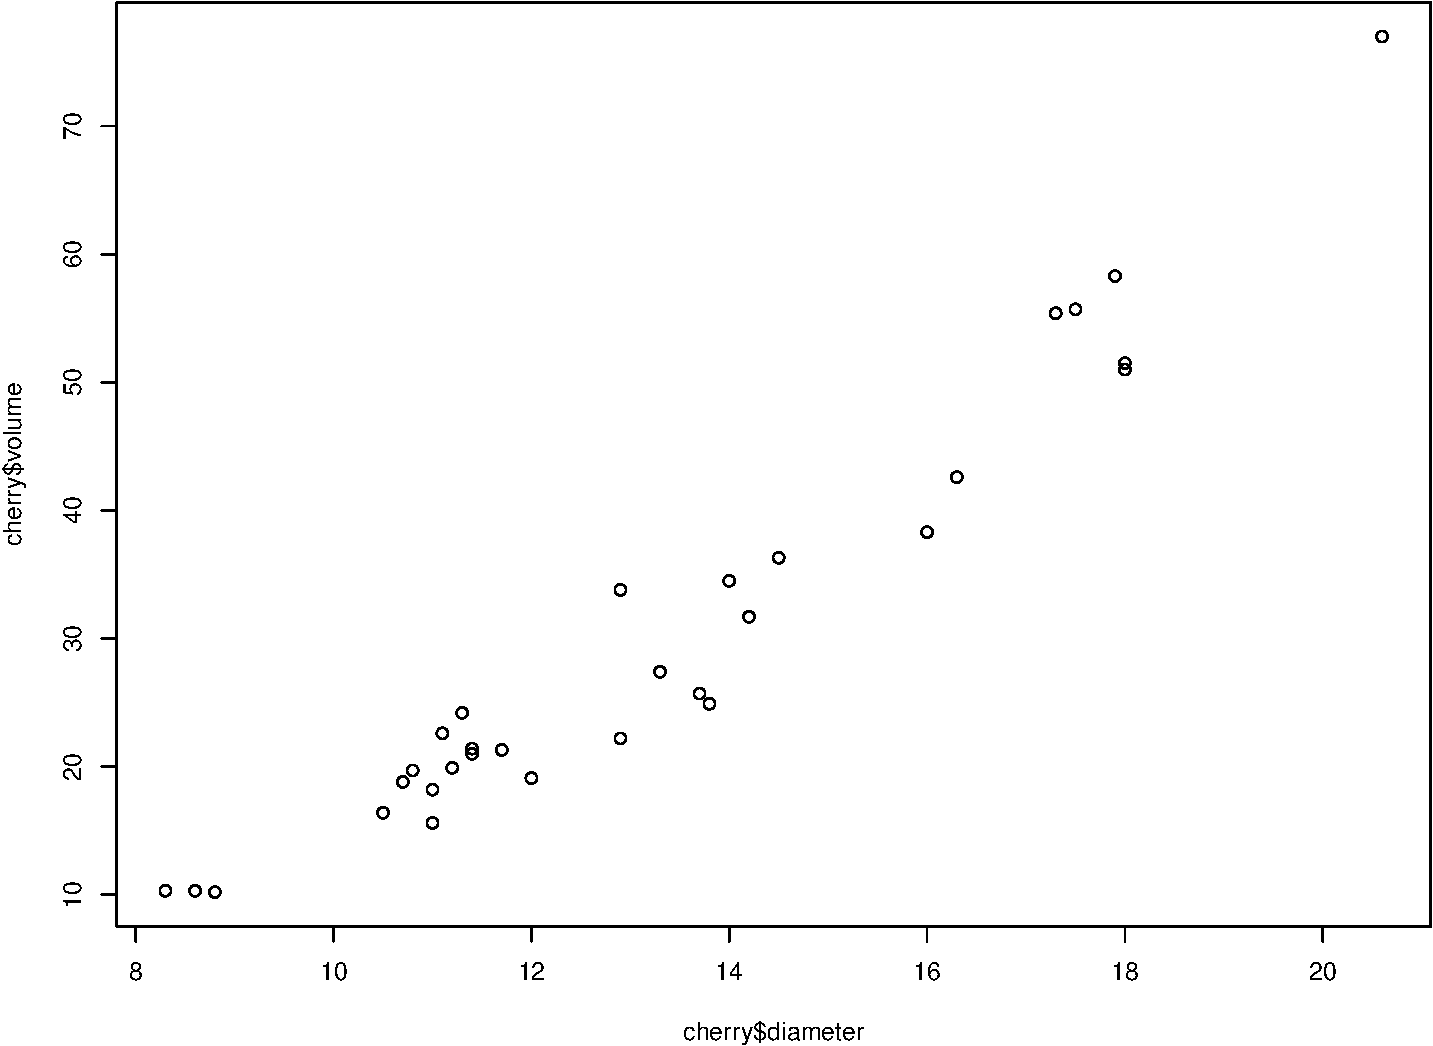
\includegraphics[keepaspectratio]{unit1-introR/introR_files/figure-pdf/unnamed-chunk-2-1.pdf}}

Produce Plots

\begin{Shaded}
\begin{Highlighting}[]
\CommentTok{\#pdf ("hist\_acres92.pdf") \#\# use this command and dev.off to save the output to a file}
\FunctionTok{hist}\NormalTok{ (agpop}\SpecialCharTok{$}\NormalTok{acres92)}
\end{Highlighting}
\end{Shaded}

\pandocbounded{\includegraphics[keepaspectratio]{unit1-introR/introR_files/figure-pdf/unnamed-chunk-3-1.pdf}}

\begin{Shaded}
\begin{Highlighting}[]
\CommentTok{\#dev.off()}

\CommentTok{\#jpeg ("agpop\_acres\_87v92.jpg")}

\FunctionTok{plot}\NormalTok{ (agpop}\SpecialCharTok{$}\NormalTok{acres87, agpop}\SpecialCharTok{$}\NormalTok{acres92)}
\FunctionTok{abline}\NormalTok{ (}\AttributeTok{a =} \DecValTok{0}\NormalTok{, }\AttributeTok{b =} \DecValTok{1}\NormalTok{)}
\end{Highlighting}
\end{Shaded}

\pandocbounded{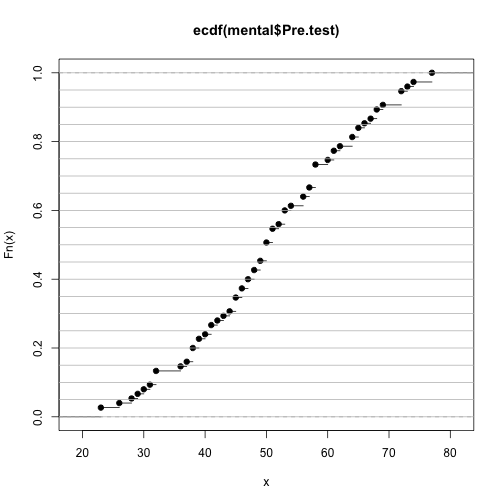
\includegraphics[keepaspectratio]{unit1-introR/introR_files/figure-pdf/unnamed-chunk-3-2.pdf}}

\begin{Shaded}
\begin{Highlighting}[]
\CommentTok{\#dev.off()\#\# this is used to close the jpeg file}
\end{Highlighting}
\end{Shaded}

\section{Create your own function}\label{create-your-own-function}

\begin{Shaded}
\begin{Highlighting}[]
\DocumentationTok{\#\# data is a matrix or data.frame}
\NormalTok{means\_col }\OtherTok{\textless{}{-}} \ControlFlowTok{function}\NormalTok{ (data)}
\NormalTok{\{}
\NormalTok{    n }\OtherTok{\textless{}{-}} \FunctionTok{ncol}\NormalTok{ (data)}
\NormalTok{    cmeans }\OtherTok{\textless{}{-}} \FunctionTok{rep}\NormalTok{ (}\ConstantTok{NA}\NormalTok{, n)}
    \ControlFlowTok{for}\NormalTok{ (j }\ControlFlowTok{in} \DecValTok{1}\SpecialCharTok{:}\NormalTok{n)}
\NormalTok{    \{}
\NormalTok{        cmeans[j] }\OtherTok{\textless{}{-}} \FunctionTok{mean}\NormalTok{ (data[,j])}
        
\NormalTok{    \}}
\NormalTok{    cmeans}
\NormalTok{\}}

\DocumentationTok{\#\# apply function}
\FunctionTok{means\_col}\NormalTok{ (agpop[, }\DecValTok{3}\SpecialCharTok{:}\DecValTok{13}\NormalTok{])}
\end{Highlighting}
\end{Shaded}

\begin{verbatim}
 [1] 306676.97141 313016.37817 320193.69298    625.50357    678.28428
 [6]    728.06238     56.17674     54.86160     52.62248     54.09227
[11]     59.53769
\end{verbatim}

\begin{Shaded}
\begin{Highlighting}[]
\DocumentationTok{\#\# R built{-}in function}
\FunctionTok{colMeans}\NormalTok{ (agpop[, }\DecValTok{3}\SpecialCharTok{:}\DecValTok{13}\NormalTok{])}
\end{Highlighting}
\end{Shaded}

\begin{verbatim}
     acres92      acres87      acres82      farms92      farms87      farms82 
306676.97141 313016.37817 320193.69298    625.50357    678.28428    728.06238 
    largef92     largef87     largef82     smallf92     smallf87 
    56.17674     54.86160     52.62248     54.09227     59.53769 
\end{verbatim}

\section{Include Images Saved in An External
File}\label{include-images-saved-in-an-external-file}

Using the following R code to include your images saved in an external
file.

\begin{Shaded}
\begin{Highlighting}[]
\NormalTok{knitr}\SpecialCharTok{::}\FunctionTok{include\_graphics}\NormalTok{(}\StringTok{"handwriting.png"}\NormalTok{)}
\end{Highlighting}
\end{Shaded}

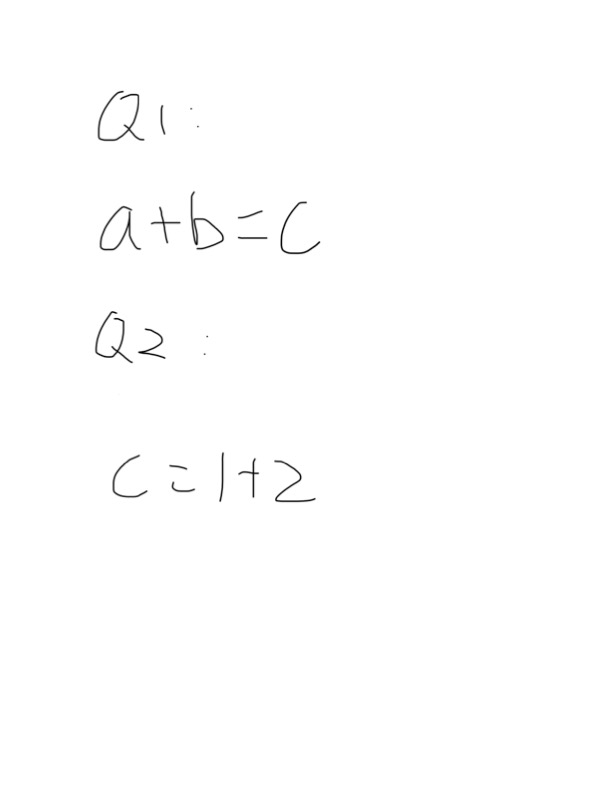
\includegraphics[width=2.04in,height=\textheight,keepaspectratio]{unit1-introR/handwriting.png}

You can hide the above R code by setting ``echo=FALSE'' for the r chunk.
For example, I will include the image once again as follows:

\begin{figure}

\centering{

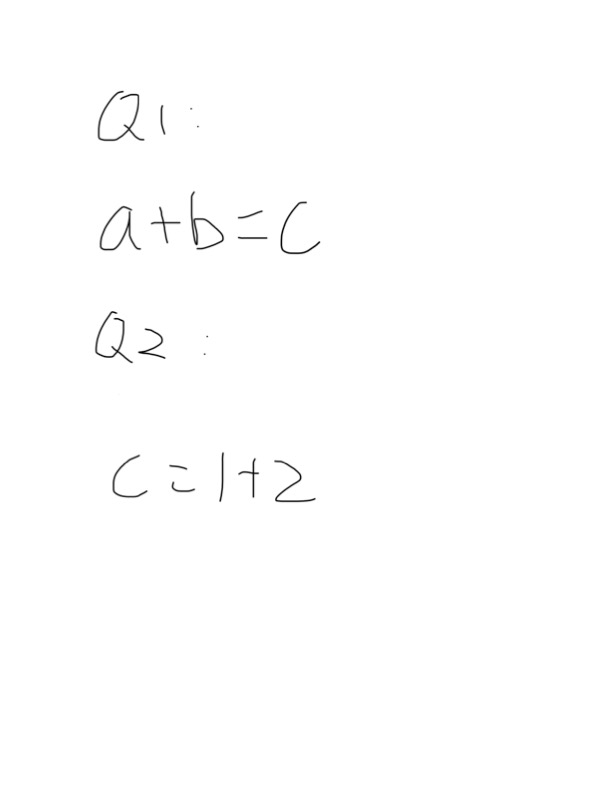
\includegraphics[width=2.04in,height=\textheight,keepaspectratio]{unit1-introR/handwriting.png}

}

\caption{\label{fig-handwriting}This is a figure inserted from the file
called ``handwriting.png''}

\end{figure}%

\section{Simple Linear Regression}\label{simple-linear-regression}

A Simulation Illustration with R

\hfill\break

\begin{Shaded}
\begin{Highlighting}[]
\FunctionTok{require}\NormalTok{(}\StringTok{"knitr"}\NormalTok{)}
\NormalTok{knitr}\SpecialCharTok{::}\NormalTok{opts\_chunk}\SpecialCharTok{$}\FunctionTok{set}\NormalTok{(}
  \AttributeTok{comment =} \StringTok{"\#"}\NormalTok{,}
  \AttributeTok{fig.width =} \DecValTok{8}\NormalTok{,}
  \AttributeTok{fig.height =} \DecValTok{6}\NormalTok{,}
  \AttributeTok{cache =} \ConstantTok{TRUE}
\NormalTok{)}
\FunctionTok{set.seed}\NormalTok{(}\DecValTok{47}\NormalTok{)}
\end{Highlighting}
\end{Shaded}

\section{Overview of Simple Linear
Regression}\label{overview-of-simple-linear-regression}

To make the simple linear regression model concrete, let's first
visualize a simulated dataset that follows \[
Y_i = \beta_0 + \beta_1 X_i + \varepsilon_i, \qquad
\varepsilon_i \sim \mathcal N(0, \sigma^2).
\]

Here, \(\beta_0\) is the intercept, \(\beta_1\) is the slope, and
\(\varepsilon_i\) represents random noise.

\begin{Shaded}
\begin{Highlighting}[]
\FunctionTok{set.seed}\NormalTok{(}\DecValTok{2025}\NormalTok{)}
\NormalTok{n }\OtherTok{\textless{}{-}} \DecValTok{40}
\NormalTok{beta0 }\OtherTok{\textless{}{-}} \DecValTok{2}\NormalTok{; beta1 }\OtherTok{\textless{}{-}} \FloatTok{1.5}\NormalTok{; sigma }\OtherTok{\textless{}{-}} \DecValTok{2}
\NormalTok{x }\OtherTok{\textless{}{-}} \FunctionTok{runif}\NormalTok{(n, }\DecValTok{0}\NormalTok{, }\DecValTok{10}\NormalTok{)}
\NormalTok{y }\OtherTok{\textless{}{-}}\NormalTok{ beta0 }\SpecialCharTok{+}\NormalTok{ beta1 }\SpecialCharTok{*}\NormalTok{ x }\SpecialCharTok{+} \FunctionTok{rnorm}\NormalTok{(n, }\DecValTok{0}\NormalTok{, sigma)}
\NormalTok{dat }\OtherTok{\textless{}{-}} \FunctionTok{data.frame}\NormalTok{(x, y)}

\NormalTok{fit }\OtherTok{\textless{}{-}} \FunctionTok{lm}\NormalTok{(y }\SpecialCharTok{\textasciitilde{}}\NormalTok{ x, }\AttributeTok{data =}\NormalTok{ dat)}

\FunctionTok{plot}\NormalTok{(x, y, }\AttributeTok{pch =} \DecValTok{19}\NormalTok{, }\AttributeTok{col =} \StringTok{"steelblue"}\NormalTok{,}
     \AttributeTok{xlab =} \StringTok{"Predictor X"}\NormalTok{, }\AttributeTok{ylab =} \StringTok{"Response Y"}\NormalTok{,}
     \AttributeTok{main =} \StringTok{"Simulated Data with Fitted Linear Regression Line"}\NormalTok{)}
\FunctionTok{abline}\NormalTok{(fit, }\AttributeTok{col =} \StringTok{"red"}\NormalTok{, }\AttributeTok{lwd =} \DecValTok{2}\NormalTok{)}
\FunctionTok{legend}\NormalTok{(}\StringTok{"topleft"}\NormalTok{, }\AttributeTok{legend =} \FunctionTok{c}\NormalTok{(}\StringTok{"Observed data"}\NormalTok{, }\StringTok{"Fitted line"}\NormalTok{),}
       \AttributeTok{pch =} \FunctionTok{c}\NormalTok{(}\DecValTok{19}\NormalTok{, }\ConstantTok{NA}\NormalTok{), }\AttributeTok{lty =} \FunctionTok{c}\NormalTok{(}\ConstantTok{NA}\NormalTok{, }\DecValTok{1}\NormalTok{), }\AttributeTok{col =} \FunctionTok{c}\NormalTok{(}\StringTok{"steelblue"}\NormalTok{, }\StringTok{"red"}\NormalTok{), }\AttributeTok{bty =} \StringTok{"n"}\NormalTok{)}
\end{Highlighting}
\end{Shaded}

\pandocbounded{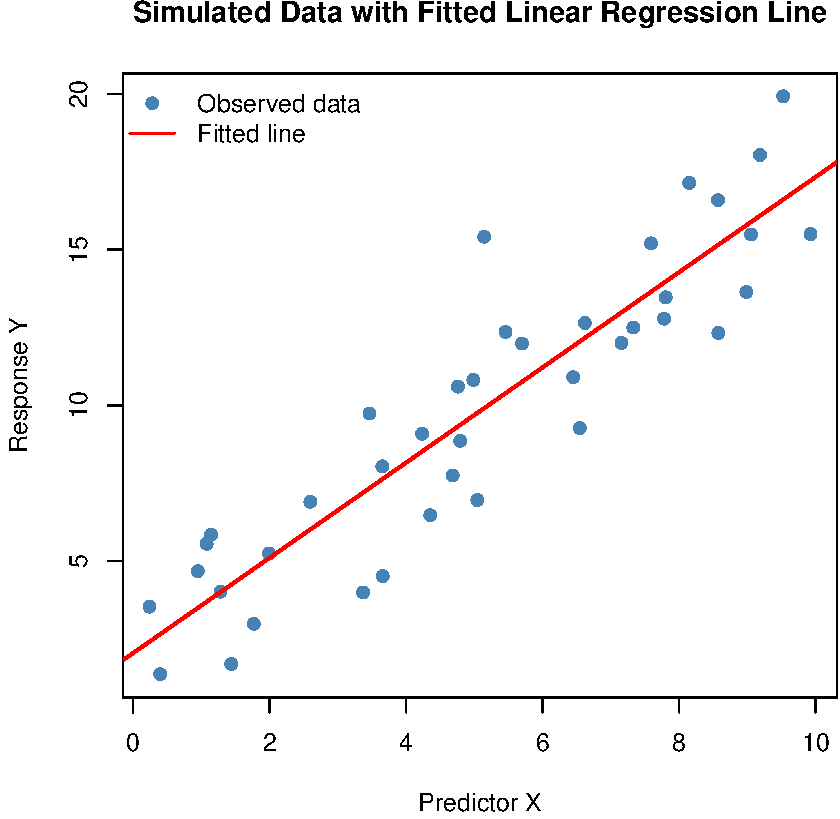
\includegraphics[keepaspectratio]{unit2-slr/slr_files/figure-pdf/unnamed-chunk-2-1.pdf}}

The scatterplot shows data points scattered around a line --- the red
line is the fitted regression model.

\begin{center}\rule{0.5\linewidth}{0.5pt}\end{center}

\subsection{Least Squares Estimation}\label{least-squares-estimation}

\textbf{Goal:} Find \(\hat\beta_0\) and \(\hat\beta_1\) that minimize \[
\mathrm{SSE} = \sum_{i=1}^n (y_i - \hat\beta_0 - \hat\beta_1 x_i)^2.
\]

\textbf{Solutions:} \[
\hat\beta_1 = \frac{\sum_i (x_i - \bar x)(y_i - \bar y)}{\sum_i (x_i - \bar x)^2}
= \frac{S_{xy}}{S_{xx}},
\qquad
\hat\beta_0 = \bar y - \hat\beta_1\,\bar x.
\]

Here \[
S_{xy} = \sum_i (x_i - \bar x)(y_i - \bar y),
\qquad
S_{xx} = \sum_i (x_i - \bar x)^2.
\]

\textbf{Shortcut (computational) formulas:} \[
S_{xy} = \sum_i x_i y_i - n\,\bar x\,\bar y,
\qquad
S_{xx} = \sum_i x_i^2 - n\,\bar x^2.
\]

\textbf{Interpretation:}\\
- \(\hat\beta_1\) measures the estimated change in \(Y\) for each unit
increase in \(X\).\\
- \(\hat\beta_0\) represents the fitted value of \(Y\) when \(X=0\).

\begin{center}\rule{0.5\linewidth}{0.5pt}\end{center}

\subsection{Residual and Sum of Squares
Definitions}\label{residual-and-sum-of-squares-definitions}

Let \(\hat y_i = \hat\beta_0 + \hat\beta_1 x_i\) and
\(e_i = y_i - \hat y_i\).

\begin{longtable}[]{@{}
  >{\raggedright\arraybackslash}p{(\linewidth - 4\tabcolsep) * \real{0.1169}}
  >{\raggedright\arraybackslash}p{(\linewidth - 4\tabcolsep) * \real{0.1688}}
  >{\raggedright\arraybackslash}p{(\linewidth - 4\tabcolsep) * \real{0.7143}}@{}}
\toprule\noalign{}
\begin{minipage}[b]{\linewidth}\raggedright
Symbol
\end{minipage} & \begin{minipage}[b]{\linewidth}\raggedright
Definition
\end{minipage} & \begin{minipage}[b]{\linewidth}\raggedright
Computing Formula (in terms of \(S_{xx}, S_{xy}\), etc.)
\end{minipage} \\
\midrule\noalign{}
\endhead
\bottomrule\noalign{}
\endlastfoot
\textbf{SST} & Total Sum of Squares &
\(\displaystyle \sum_i (y_i - \bar y)^2 = S_{yy} = \sum_i y_i^2 - n\,\bar y^2\) \\
\textbf{SSR} & Regression Sum of Squares &
\(\displaystyle \sum_i (\hat y_i - \bar y)^2 = \hat\beta_1^2 S_{xx} = \frac{S_{xy}^2}{S_{xx}}\) \\
\textbf{SSE} & Error (Residual) Sum of Squares &
\(\displaystyle \sum_i (y_i - \hat y_i)^2 = S_{yy} - \frac{S_{xy}^2}{S_{xx}}\) \\
\end{longtable}

\textbf{Identity:} \[
\mathrm{SST} = \mathrm{SSR} + \mathrm{SSE}.
\]

Here, \[
S_{xx} = \sum_i (x_i - \bar x)^2 = \sum_i x_i^2 - n\bar x^2, \qquad
S_{yy} = \sum_i (y_i - \bar y)^2 = \sum_i y_i^2 - n\bar y^2, \qquad
S_{xy} = \sum_i (x_i - \bar x)(y_i - \bar y) = \sum_i x_i y_i - n\bar x \bar y.
\]

\begin{center}\rule{0.5\linewidth}{0.5pt}\end{center}

\subsection{\texorpdfstring{Coefficient of Determination
(\(R^2\))}{Coefficient of Determination (R\^{}2)}}\label{coefficient-of-determination-r2}

Measures the proportion of total variation in \(Y\) explained by \(X\):
\[
R^2 = \frac{\mathrm{SSR}}{\mathrm{SST}}
= 1 - \frac{\mathrm{SSE}}{\mathrm{SST}}.
\]

\textbf{Interpretation:}

\begin{itemize}
\tightlist
\item
  \(R^2 = 1\) means perfect linear fit;
\item
  \(R^2 = 0\) means the model explains none of the variation.
\end{itemize}

\begin{center}\rule{0.5\linewidth}{0.5pt}\end{center}

\subsection{F-test for Overall
Significance}\label{f-test-for-overall-significance}

Tests whether \(X\) is linearly related to \(Y\).

\textbf{Hypotheses:} \[
H_0: \beta_1 = 0
\quad \text{vs.} \quad
H_A: \beta_1 \ne 0.
\]

\textbf{Test Statistic:} \[
F = \frac{\text{MSR}}{\text{MSE}}
= \frac{\text{SSR}/1}{\text{SSE}/(n-2)}
\sim F_{1,n-2}\quad (H_0).
\]

\textbf{p-value approach for observe \(F^{\mathrm{obs}}\):}

Given the observed statistic (F\^{}\{\text{obs}\}) with ((1,,n-2)) df,
\[
p-\text{value} \;=\; \Pr\!\big(F_{1,\,n-2} \ge F^{\text{obs}}\big)
\;=\; \mathrm{pf}\!\big(F^{\text{obs}},\,1,\,n-2,\ \text{lower.tail}= \mathrm{FALSE}\big).
\]

\begin{Shaded}
\begin{Highlighting}[]
\CommentTok{\# {-}{-} Inputs (provide these from your analysis context) {-}{-}{-}{-}{-}{-}{-}{-}{-}{-}{-}{-}{-}{-}{-}{-}{-}{-}{-}{-}{-}{-}{-}{-}{-}}
\CommentTok{\# n   \textless{}{-} ...   \# sample size}
\CommentTok{\# SSR \textless{}{-} ...   \# regression sum of squares}
\CommentTok{\# SSE \textless{}{-} ...   \# error sum of squares}
\NormalTok{n   }\OtherTok{\textless{}{-}} \DecValTok{20}
\NormalTok{SSR }\OtherTok{\textless{}{-}} \DecValTok{5}
\NormalTok{SSE }\OtherTok{\textless{}{-}} \DecValTok{40}




\NormalTok{df1  }\OtherTok{\textless{}{-}} \DecValTok{1}
\NormalTok{df2  }\OtherTok{\textless{}{-}}\NormalTok{ n }\SpecialCharTok{{-}} \DecValTok{2}
\NormalTok{Fobs }\OtherTok{\textless{}{-}}\NormalTok{ (SSR}\SpecialCharTok{/}\NormalTok{df1) }\SpecialCharTok{/}\NormalTok{ (SSE}\SpecialCharTok{/}\NormalTok{df2)         }\CommentTok{\# observed F}
\NormalTok{pval }\OtherTok{\textless{}{-}} \FunctionTok{pf}\NormalTok{(Fobs, }\AttributeTok{df1 =}\NormalTok{ df1, }\AttributeTok{df2 =}\NormalTok{ df2, }\AttributeTok{lower.tail =} \ConstantTok{FALSE}\NormalTok{)}
\NormalTok{pval}
\end{Highlighting}
\end{Shaded}

\begin{verbatim}
[1] 0.1509505
\end{verbatim}

\begin{Shaded}
\begin{Highlighting}[]
\CommentTok{\# {-}{-} Plot F density and shade the p{-}value tail (with proper annotations) {-}{-}{-}{-}{-}{-}{-}}
\NormalTok{xmax }\OtherTok{\textless{}{-}} \FunctionTok{max}\NormalTok{(}\FunctionTok{qf}\NormalTok{(}\FloatTok{0.995}\NormalTok{, df1, df2), Fobs }\SpecialCharTok{*} \FloatTok{1.2}\NormalTok{)  }\CommentTok{\# extra space for labels}
\NormalTok{peak }\OtherTok{\textless{}{-}} \FunctionTok{max}\NormalTok{(}\FunctionTok{df}\NormalTok{(}\FunctionTok{seq}\NormalTok{(}\DecValTok{0}\NormalTok{, xmax, }\AttributeTok{length.out =} \DecValTok{500}\NormalTok{), df1, df2))}

\CommentTok{\# Density curve}
\FunctionTok{curve}\NormalTok{(}\FunctionTok{df}\NormalTok{(x, df1, df2), }\AttributeTok{from =} \DecValTok{0}\NormalTok{, }\AttributeTok{to =}\NormalTok{ xmax,}
      \AttributeTok{xlab =} \StringTok{"F"}\NormalTok{, }\AttributeTok{ylab =} \StringTok{"Density"}\NormalTok{,}
      \AttributeTok{main =} \FunctionTok{sprintf}\NormalTok{(}\StringTok{"F(\%d, \%d) density  |  observed F = \%.3f"}\NormalTok{, df1, df2, Fobs))}

\CommentTok{\# Shade right tail (p{-}value region)}
\NormalTok{xs }\OtherTok{\textless{}{-}} \FunctionTok{seq}\NormalTok{(Fobs, xmax, }\AttributeTok{length.out =} \DecValTok{300}\NormalTok{)}
\NormalTok{ys }\OtherTok{\textless{}{-}} \FunctionTok{df}\NormalTok{(xs, df1, df2)}
\FunctionTok{polygon}\NormalTok{(}\FunctionTok{c}\NormalTok{(Fobs, xs, xmax), }\FunctionTok{c}\NormalTok{(}\DecValTok{0}\NormalTok{, ys, }\DecValTok{0}\NormalTok{),}
        \AttributeTok{col =} \FunctionTok{rgb}\NormalTok{(}\DecValTok{0}\NormalTok{, }\DecValTok{0}\NormalTok{, }\DecValTok{0}\NormalTok{, }\FloatTok{0.18}\NormalTok{), }\AttributeTok{border =} \ConstantTok{NA}\NormalTok{)}

\CommentTok{\# Vertical line at Fobs (optional visual aid)}
\FunctionTok{abline}\NormalTok{(}\AttributeTok{v =}\NormalTok{ Fobs, }\AttributeTok{lwd =} \DecValTok{2}\NormalTok{)}

\CommentTok{\# {-}{-}{-}{-} Annotation for F\^{}obs pointing to the x{-}axis value (Fobs, 0) {-}{-}{-}{-}{-}{-}{-}{-}{-}{-}{-}{-}{-}}
\NormalTok{x\_txt\_F }\OtherTok{\textless{}{-}}\NormalTok{ Fobs }\SpecialCharTok{+} \FloatTok{0.06} \SpecialCharTok{*}\NormalTok{ xmax}
\NormalTok{y\_txt\_F }\OtherTok{\textless{}{-}} \FloatTok{0.45} \SpecialCharTok{*}\NormalTok{ peak}
\FunctionTok{arrows}\NormalTok{(}\AttributeTok{x0 =}\NormalTok{ x\_txt\_F, }\AttributeTok{y0 =}\NormalTok{ y\_txt\_F, }\AttributeTok{x1 =}\NormalTok{ Fobs, }\AttributeTok{y1 =} \DecValTok{0}\NormalTok{,}
       \AttributeTok{length =} \FloatTok{0.08}\NormalTok{, }\AttributeTok{lwd =} \FloatTok{1.5}\NormalTok{)}
\FunctionTok{text}\NormalTok{(x\_txt\_F, y\_txt\_F,}
     \AttributeTok{labels =} \FunctionTok{bquote}\NormalTok{(F}\SpecialCharTok{\^{}}\NormalTok{\{obs\} }\SpecialCharTok{==}\NormalTok{ .(}\FunctionTok{format}\NormalTok{(Fobs, }\AttributeTok{digits =} \DecValTok{3}\NormalTok{))),}
     \AttributeTok{pos =} \DecValTok{4}\NormalTok{)}

\CommentTok{\# {-}{-}{-}{-} Annotation for p{-}value pointing into the shaded tail {-}{-}{-}{-}{-}{-}{-}{-}{-}{-}{-}{-}{-}{-}{-}{-}{-}{-}{-}{-}}
\NormalTok{x\_tip\_p }\OtherTok{\textless{}{-}}\NormalTok{ (Fobs }\SpecialCharTok{+}\NormalTok{ xmax) }\SpecialCharTok{/} \FloatTok{1.7}
\NormalTok{y\_tip\_p }\OtherTok{\textless{}{-}} \FunctionTok{df}\NormalTok{(x\_tip\_p, df1, df2)}
\NormalTok{x\_txt\_p }\OtherTok{\textless{}{-}}\NormalTok{ Fobs }\SpecialCharTok{+} \FloatTok{0.08} \SpecialCharTok{*}\NormalTok{ xmax}
\NormalTok{y\_txt\_p }\OtherTok{\textless{}{-}} \FloatTok{0.80} \SpecialCharTok{*}\NormalTok{ peak}
\FunctionTok{arrows}\NormalTok{(}\AttributeTok{x0 =}\NormalTok{ x\_txt\_p, }\AttributeTok{y0 =}\NormalTok{ y\_txt\_p, }\AttributeTok{x1 =}\NormalTok{ x\_tip\_p, }\AttributeTok{y1 =}\NormalTok{ y\_tip\_p,}
       \AttributeTok{length =} \FloatTok{0.08}\NormalTok{, }\AttributeTok{lwd =} \FloatTok{1.5}\NormalTok{)}
\FunctionTok{text}\NormalTok{(x\_txt\_p, y\_txt\_p,}
     \AttributeTok{labels =} \FunctionTok{bquote}\NormalTok{(p }\SpecialCharTok{==}\NormalTok{ .(}\FunctionTok{format}\NormalTok{(pval, }\AttributeTok{digits =} \DecValTok{4}\NormalTok{, }\AttributeTok{scientific =} \ConstantTok{TRUE}\NormalTok{))),}
     \AttributeTok{pos =} \DecValTok{4}\NormalTok{)}
\end{Highlighting}
\end{Shaded}

\pandocbounded{\includegraphics[keepaspectratio]{unit2-slr/slr_files/figure-pdf/unnamed-chunk-3-1.pdf}}

\begin{center}\rule{0.5\linewidth}{0.5pt}\end{center}

\subsection{\texorpdfstring{t-test for the Slope
\(\beta_1\)}{t-test for the Slope \textbackslash beta\_1}}\label{t-test-for-the-slope-beta_1}

Equivalent to the \(F\)-test in simple regression since \(t^2 = F\).

\textbf{Formula:} \[
t = \frac{\hat\beta_1}{\operatorname{SE}(\hat\beta_1)},
\qquad
\operatorname{SE}(\hat\beta_1) = \sqrt{\frac{\hat\sigma^2}{\sum_i (x_i - \bar x)^2}},
\qquad
\hat\sigma^2 = \frac{\mathrm{SSE}}{n-2}.
\]

\textbf{Distribution:} \[
t \sim t_{n-2}\quad (H_0:\beta_1=0).
\]

\begin{center}\rule{0.5\linewidth}{0.5pt}\end{center}

\subsection{\texorpdfstring{Prediction for a New Case
\(x_0\)}{Prediction for a New Case x\_0}}\label{prediction-for-a-new-case-x_0}

\textbf{Predicted mean response:} \[
\hat y(x_0) = \hat\beta_0 + \hat\beta_1 x_0.
\]

\textbf{95\% Confidence interval for mean response:} \[
\hat y(x_0) \pm t_{1-\alpha/2,,n-2},
\hat\sigma,\sqrt{\frac{1}{n} + \frac{(x_0 - \bar x)^2}{\sum_i (x_i - \bar x)^2}}.
\]

\textbf{95\% Prediction interval for a new observation:} \[
\hat y(x_0) \pm t_{1-\alpha/2,,n-2},
\hat\sigma,\sqrt{1 + \frac{1}{n} + \frac{(x_0 - \bar x)^2}{\sum_i (x_i - \bar x)^2}}.
\]

\begin{center}\rule{0.5\linewidth}{0.5pt}\end{center}

\textbf{Summary Cheat Sheet}

\begin{longtable}[]{@{}
  >{\raggedright\arraybackslash}p{(\linewidth - 2\tabcolsep) * \real{0.1512}}
  >{\raggedright\arraybackslash}p{(\linewidth - 2\tabcolsep) * \real{0.8488}}@{}}
\toprule\noalign{}
\begin{minipage}[b]{\linewidth}\raggedright
Concept
\end{minipage} & \begin{minipage}[b]{\linewidth}\raggedright
Key Formula
\end{minipage} \\
\midrule\noalign{}
\endhead
\bottomrule\noalign{}
\endlastfoot
Model & \(Y_i = \beta_0 + \beta_1 X_i + \varepsilon_i\) \\
LS Estimates & \(\hat\beta_1 = S_{xy}/S_{xx}\),
\(\hat\beta_0 = \bar y - \hat\beta_1\bar x\) \\
Decomposition & \(\mathrm{SST} = \mathrm{SSR} + \mathrm{SSE}\) \\
\(R^2\) & \(R^2 = 1 - \mathrm{SSE}/\mathrm{SST}\) \\
\(F\)-test & \(F = (\mathrm{SSR}/1)/(\mathrm{SSE}/(n-2))\) \\
\(t\)-test & \(t = \hat\beta_1 / \operatorname{SE}(\hat\beta_1)\) \\
Prediction & \(\hat y(x_0) = \hat\beta_0 + \hat\beta_1 x_0\) \\
\end{longtable}

\section{Example 1: Vehicle Insurance Premium
(warm-up)}\label{example-1-vehicle-insurance-premium-warm-up}

We examine premiums \(y\) vs.~driving amount \(x\). The scatterplot
hints at a \textbf{downward} trend.

\subsection{Input data}\label{input-data}

\begin{Shaded}
\begin{Highlighting}[]
\NormalTok{issu }\OtherTok{\textless{}{-}} \FunctionTok{data.frame}\NormalTok{(}
  \AttributeTok{driving =} \FunctionTok{c}\NormalTok{(}\DecValTok{5}\NormalTok{, }\DecValTok{2}\NormalTok{, }\DecValTok{12}\NormalTok{, }\DecValTok{9}\NormalTok{, }\DecValTok{15}\NormalTok{, }\DecValTok{6}\NormalTok{, }\DecValTok{25}\NormalTok{, }\DecValTok{16}\NormalTok{),}
  \AttributeTok{premium =} \FunctionTok{c}\NormalTok{(}\DecValTok{64}\NormalTok{, }\DecValTok{87}\NormalTok{, }\DecValTok{50}\NormalTok{, }\DecValTok{71}\NormalTok{, }\DecValTok{44}\NormalTok{, }\DecValTok{56}\NormalTok{, }\DecValTok{42}\NormalTok{, }\DecValTok{60}\NormalTok{)}
\NormalTok{)}

\NormalTok{y }\OtherTok{\textless{}{-}}\NormalTok{ issu}\SpecialCharTok{$}\NormalTok{premium}
\NormalTok{x }\OtherTok{\textless{}{-}}\NormalTok{ issu}\SpecialCharTok{$}\NormalTok{driving}
\NormalTok{xbar }\OtherTok{\textless{}{-}} \FunctionTok{mean}\NormalTok{(x); ybar }\OtherTok{\textless{}{-}} \FunctionTok{mean}\NormalTok{(y); n }\OtherTok{\textless{}{-}} \FunctionTok{length}\NormalTok{(y)}

\FunctionTok{plot}\NormalTok{(x, y, }\AttributeTok{xlab =} \StringTok{"Driving"}\NormalTok{, }\AttributeTok{ylab =} \StringTok{"Premium"}\NormalTok{,}
     \AttributeTok{main =} \StringTok{"Vehicle Insurance: Premium vs. Driving"}\NormalTok{)}
\FunctionTok{abline}\NormalTok{(}\AttributeTok{h =}\NormalTok{ ybar, }\AttributeTok{lty =} \DecValTok{3}\NormalTok{)}
\end{Highlighting}
\end{Shaded}

\pandocbounded{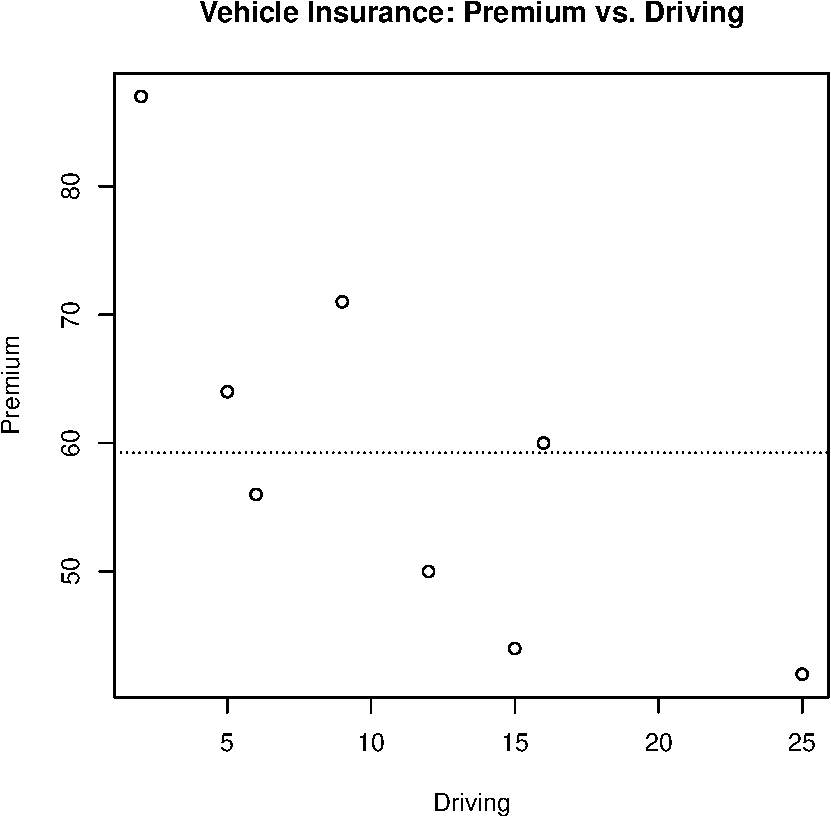
\includegraphics[keepaspectratio]{unit2-slr/slr_files/figure-pdf/unnamed-chunk-4-1.pdf}}

\textbf{Narrative.} The horizontal line at \(\bar y\) represents the
intercept-only model. Any fitted line that tilts away from this must
earn its keep by reducing residual variation enough to offset the loss
of one degree of freedom.

\subsection{Estimating regression
coefficients}\label{estimating-regression-coefficients}

\begin{Shaded}
\begin{Highlighting}[]
\NormalTok{fit.issu }\OtherTok{\textless{}{-}} \FunctionTok{lm}\NormalTok{(y }\SpecialCharTok{\textasciitilde{}}\NormalTok{ x)}
\FunctionTok{plot}\NormalTok{(x, y, }\AttributeTok{xlab =} \StringTok{"Driving"}\NormalTok{, }\AttributeTok{ylab =} \StringTok{"Premium"}\NormalTok{,}
     \AttributeTok{main =} \StringTok{"Fitted Simple Linear Regression"}\NormalTok{)}
\FunctionTok{abline}\NormalTok{(fit.issu, }\AttributeTok{lwd =} \DecValTok{2}\NormalTok{)}
\end{Highlighting}
\end{Shaded}

\pandocbounded{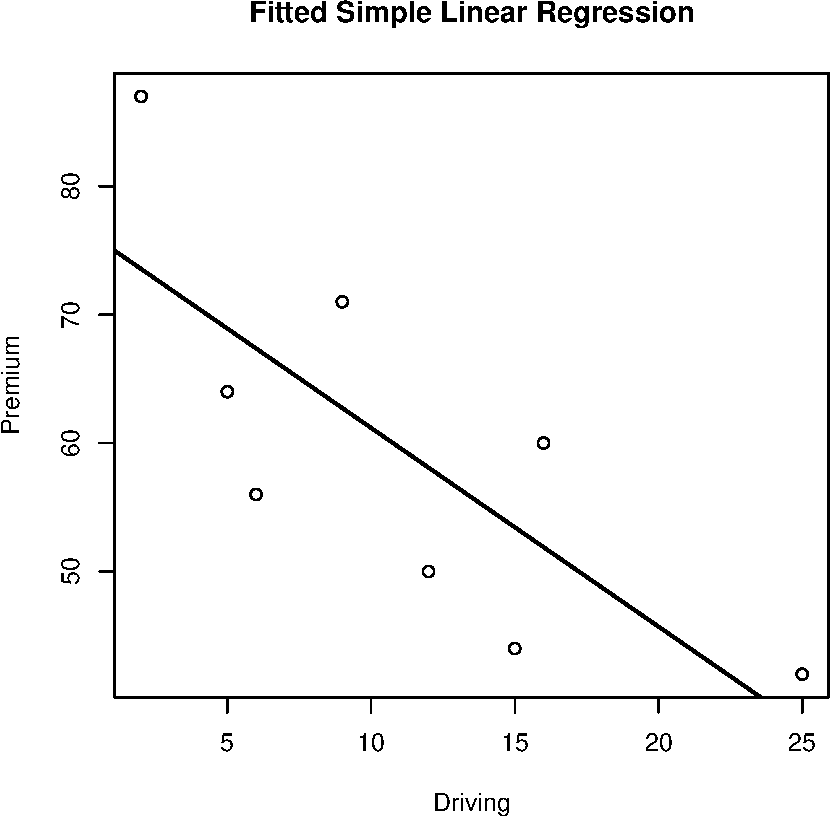
\includegraphics[keepaspectratio]{unit2-slr/slr_files/figure-pdf/unnamed-chunk-5-1.pdf}}

The slope estimate \(\hat\beta_1\) captures the \textbf{marginal change
in premium per unit of driving} (units of \(y\) per unit of \(x\)).
Inference on \(\beta_1\) tells us whether the pattern rises above noise.

\subsection{Residuals and fitted values (geometry
picture)}\label{residuals-and-fitted-values-geometry-picture}

Let \(\hat y_i=\hat\beta_0+\hat\beta_1 x_i\) and \(\tilde y_i=\bar y\).
Residuals are \(e_i=y_i-\hat y_i\) (model) and \(y_i-\bar y\) (null).
Visualizing all three clarifies the ANOVA identity.

\begin{Shaded}
\begin{Highlighting}[]
\NormalTok{beta0 }\OtherTok{\textless{}{-}} \FunctionTok{coef}\NormalTok{(fit.issu)[}\DecValTok{1}\NormalTok{]}
\NormalTok{beta1 }\OtherTok{\textless{}{-}} \FunctionTok{coef}\NormalTok{(fit.issu)[}\DecValTok{2}\NormalTok{]}
\NormalTok{fitted1 }\OtherTok{\textless{}{-}}\NormalTok{ beta0 }\SpecialCharTok{+}\NormalTok{ beta1 }\SpecialCharTok{*}\NormalTok{ x}
\NormalTok{fitted0 }\OtherTok{\textless{}{-}} \FunctionTok{rep}\NormalTok{(ybar, n)}
\NormalTok{residual1 }\OtherTok{\textless{}{-}}\NormalTok{ y }\SpecialCharTok{{-}}\NormalTok{ fitted1}
\NormalTok{residual0 }\OtherTok{\textless{}{-}}\NormalTok{ y }\SpecialCharTok{{-}}\NormalTok{ fitted0}

\FunctionTok{data.frame}\NormalTok{(y, fitted0, residual0, fitted1, residual1,}
           \AttributeTok{diff.fitted =}\NormalTok{ fitted1 }\SpecialCharTok{{-}}\NormalTok{ fitted0)}
\end{Highlighting}
\end{Shaded}

\begin{verbatim}
   y fitted0 residual0  fitted1  residual1 diff.fitted
1 64   59.25      4.75 68.92243  -4.922425    9.672425
2 87   59.25     27.75 73.56519  13.434811   14.315189
3 50   59.25     -9.25 58.08931  -8.089309   -1.160691
4 71   59.25     11.75 62.73207   8.267927    3.482073
5 44   59.25    -15.25 53.44654  -9.446545   -5.803455
6 56   59.25     -3.25 67.37484 -11.374837    8.124837
7 42   59.25    -17.25 37.97066   4.029335  -21.279335
8 60   59.25      0.75 51.89896   8.101043   -7.351043
\end{verbatim}

\pandocbounded{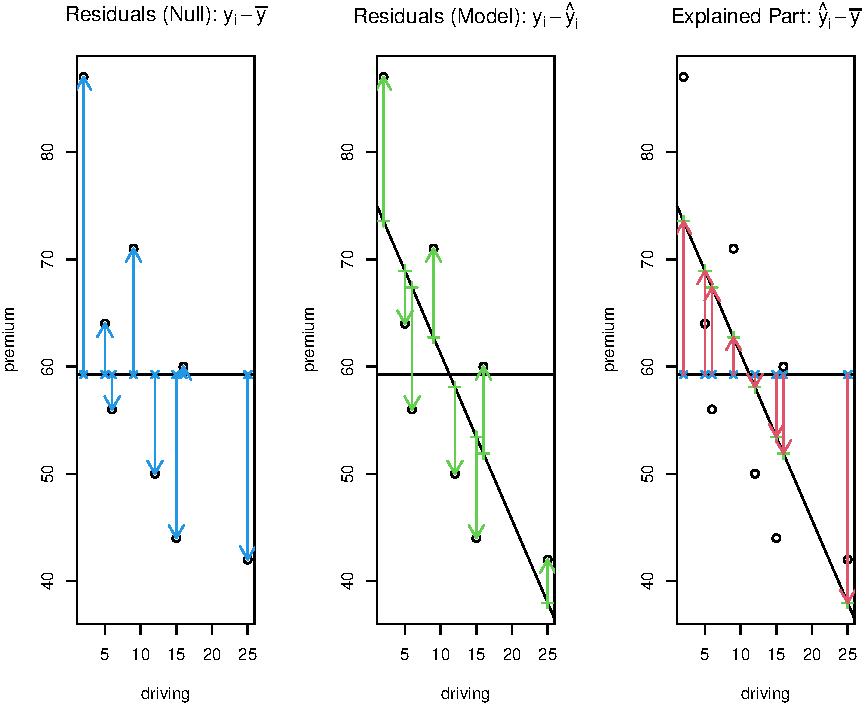
\includegraphics[keepaspectratio]{unit2-slr/slr_files/figure-pdf/unnamed-chunk-7-1.pdf}}

\subsection{SST, SSR, SSE and their
meanings}\label{sst-ssr-sse-and-their-meanings}

\begin{itemize}
\tightlist
\item
  \(\text{SST}=\sum (y_i-\bar y)^2\) quantifies \textbf{total}
  variability around the mean.
\item
  \(\text{SSR}=\sum (\hat y_i-\bar y)^2\) is the part \textbf{explained
  by \(x\)}.
\item
  \(\text{SSE}=\sum (y_i-\hat y_i)^2\) is the \textbf{leftover}
  (unexplained) variability.
\end{itemize}

\begin{Shaded}
\begin{Highlighting}[]
\NormalTok{SST }\OtherTok{\textless{}{-}} \FunctionTok{sum}\NormalTok{((y }\SpecialCharTok{{-}}\NormalTok{ fitted0)}\SpecialCharTok{\^{}}\DecValTok{2}\NormalTok{); SST}
\end{Highlighting}
\end{Shaded}

\begin{verbatim}
[1] 1557.5
\end{verbatim}

\begin{Shaded}
\begin{Highlighting}[]
\NormalTok{SSE }\OtherTok{\textless{}{-}} \FunctionTok{sum}\NormalTok{((y }\SpecialCharTok{{-}}\NormalTok{ fitted1)}\SpecialCharTok{\^{}}\DecValTok{2}\NormalTok{); SSE}
\end{Highlighting}
\end{Shaded}

\begin{verbatim}
[1] 639.0065
\end{verbatim}

\begin{Shaded}
\begin{Highlighting}[]
\NormalTok{SSR }\OtherTok{\textless{}{-}}\NormalTok{ SST }\SpecialCharTok{{-}}\NormalTok{ SSE; SSR}
\end{Highlighting}
\end{Shaded}

\begin{verbatim}
[1] 918.4935
\end{verbatim}

Direct check: \(\text{SSR}=\sum(\hat y_i-\bar y)^2\).

\begin{Shaded}
\begin{Highlighting}[]
\FunctionTok{sum}\NormalTok{((fitted1 }\SpecialCharTok{{-}}\NormalTok{ fitted0)}\SpecialCharTok{\^{}}\DecValTok{2}\NormalTok{)}
\end{Highlighting}
\end{Shaded}

\begin{verbatim}
[1] 918.4935
\end{verbatim}

\subsection{Visual ANOVA on an RSS
plot}\label{visual-anova-on-an-rss-plot}

We place the \textbf{residual sum of squares} against model dimension to
show the trade-off between fit and df.

\begin{Shaded}
\begin{Highlighting}[]
\CommentTok{\# Recompute cleanly}
\NormalTok{SST }\OtherTok{\textless{}{-}} \FunctionTok{sum}\NormalTok{((y }\SpecialCharTok{{-}} \FunctionTok{mean}\NormalTok{(y))}\SpecialCharTok{\^{}}\DecValTok{2}\NormalTok{)}
\NormalTok{SSE }\OtherTok{\textless{}{-}} \FunctionTok{sum}\NormalTok{(}\FunctionTok{resid}\NormalTok{(fit.issu)}\SpecialCharTok{\^{}}\DecValTok{2}\NormalTok{)}
\NormalTok{SSR }\OtherTok{\textless{}{-}}\NormalTok{ SST }\SpecialCharTok{{-}}\NormalTok{ SSE}
\NormalTok{df\_SSR }\OtherTok{\textless{}{-}} \DecValTok{1}
\NormalTok{df\_SSE }\OtherTok{\textless{}{-}}\NormalTok{ n }\SpecialCharTok{{-}} \DecValTok{2}

\FunctionTok{par}\NormalTok{(}\AttributeTok{mar =} \FunctionTok{c}\NormalTok{(}\DecValTok{6}\NormalTok{, }\DecValTok{4}\NormalTok{, }\DecValTok{4}\NormalTok{, }\DecValTok{2}\NormalTok{) }\SpecialCharTok{+} \FloatTok{0.1}\NormalTok{)}
\FunctionTok{plot}\NormalTok{(}\FunctionTok{c}\NormalTok{(}\DecValTok{1}\NormalTok{, }\DecValTok{2}\NormalTok{, n), }\FunctionTok{c}\NormalTok{(SST, SSE, }\DecValTok{0}\NormalTok{), }\AttributeTok{type =} \StringTok{"b"}\NormalTok{, }\AttributeTok{pch =} \DecValTok{19}\NormalTok{,}
     \AttributeTok{xlab =} \StringTok{"Number of Parameters in Model"}\NormalTok{,}
     \AttributeTok{ylab =} \StringTok{"Residual Sum of Squares (RSS)"}\NormalTok{,}
     \AttributeTok{main =} \StringTok{"ANOVA Geometry on RSS vs. Model Size"}\NormalTok{,}
     \AttributeTok{xlim =} \FunctionTok{c}\NormalTok{(}\DecValTok{0}\NormalTok{, }\DecValTok{14}\NormalTok{), }\AttributeTok{ylim =} \FunctionTok{c}\NormalTok{(}\SpecialCharTok{{-}}\DecValTok{400}\NormalTok{, SST }\SpecialCharTok{*} \FloatTok{1.1}\NormalTok{), }\AttributeTok{xaxt =} \StringTok{"n"}\NormalTok{)}
\FunctionTok{axis}\NormalTok{(}\DecValTok{1}\NormalTok{, }\AttributeTok{at =} \FunctionTok{c}\NormalTok{(}\DecValTok{1}\NormalTok{, }\DecValTok{2}\NormalTok{, n), }\AttributeTok{labels =} \FunctionTok{c}\NormalTok{(}\StringTok{"1 (Intercept)"}\NormalTok{, }\StringTok{"2 (+Slope)"}\NormalTok{, }\FunctionTok{paste}\NormalTok{(n, }\StringTok{"(Saturated)"}\NormalTok{)))}
\FunctionTok{abline}\NormalTok{(}\AttributeTok{h =} \FunctionTok{seq}\NormalTok{(}\DecValTok{0}\NormalTok{, }\DecValTok{2000}\NormalTok{, }\AttributeTok{by =} \DecValTok{100}\NormalTok{), }\AttributeTok{lty =} \DecValTok{3}\NormalTok{, }\AttributeTok{col =} \StringTok{"grey"}\NormalTok{)}

\FunctionTok{par}\NormalTok{(}\AttributeTok{xpd =} \ConstantTok{TRUE}\NormalTok{)}
\FunctionTok{arrows}\NormalTok{(}\DecValTok{9}\NormalTok{, }\DecValTok{0}\NormalTok{, }\DecValTok{9}\NormalTok{, SSE, }\AttributeTok{col =} \StringTok{"blue"}\NormalTok{, }\AttributeTok{code =} \DecValTok{3}\NormalTok{, }\AttributeTok{angle =} \DecValTok{90}\NormalTok{, }\AttributeTok{length =} \FloatTok{0.1}\NormalTok{, }\AttributeTok{lwd =} \DecValTok{2}\NormalTok{)}
\FunctionTok{text}\NormalTok{(}\DecValTok{9}\NormalTok{, SSE}\SpecialCharTok{/}\DecValTok{2}\NormalTok{, }\StringTok{"SSE"}\NormalTok{, }\AttributeTok{col =} \StringTok{"blue"}\NormalTok{, }\AttributeTok{pos =} \DecValTok{4}\NormalTok{, }\AttributeTok{font =} \DecValTok{2}\NormalTok{, }\AttributeTok{cex =} \FloatTok{1.2}\NormalTok{)}

\FunctionTok{arrows}\NormalTok{(}\DecValTok{9}\NormalTok{, SSE, }\DecValTok{9}\NormalTok{, SST, }\AttributeTok{col =} \StringTok{"red"}\NormalTok{, }\AttributeTok{code =} \DecValTok{3}\NormalTok{, }\AttributeTok{angle =} \DecValTok{90}\NormalTok{, }\AttributeTok{length =} \FloatTok{0.1}\NormalTok{, }\AttributeTok{lwd =} \DecValTok{2}\NormalTok{)}
\FunctionTok{text}\NormalTok{(}\DecValTok{9}\NormalTok{, (SST }\SpecialCharTok{+}\NormalTok{ SSE)}\SpecialCharTok{/}\DecValTok{2}\NormalTok{, }\StringTok{"SSR"}\NormalTok{, }\AttributeTok{col =} \StringTok{"red"}\NormalTok{, }\AttributeTok{pos =} \DecValTok{4}\NormalTok{, }\AttributeTok{font =} \DecValTok{2}\NormalTok{, }\AttributeTok{cex =} \FloatTok{1.2}\NormalTok{)}

\FunctionTok{arrows}\NormalTok{(}\DecValTok{2}\NormalTok{, }\SpecialCharTok{{-}}\DecValTok{200}\NormalTok{, n, }\SpecialCharTok{{-}}\DecValTok{200}\NormalTok{, }\AttributeTok{col =} \StringTok{"blue"}\NormalTok{, }\AttributeTok{code =} \DecValTok{3}\NormalTok{, }\AttributeTok{angle =} \DecValTok{90}\NormalTok{, }\AttributeTok{length =} \FloatTok{0.1}\NormalTok{, }\AttributeTok{lwd =} \DecValTok{2}\NormalTok{)}
\FunctionTok{text}\NormalTok{((}\DecValTok{2} \SpecialCharTok{+}\NormalTok{ n)}\SpecialCharTok{/}\DecValTok{2}\NormalTok{, }\SpecialCharTok{{-}}\DecValTok{250}\NormalTok{, }\FunctionTok{paste}\NormalTok{(}\StringTok{"df\_SSE ="}\NormalTok{, df\_SSE), }\AttributeTok{col =} \StringTok{"blue"}\NormalTok{, }\AttributeTok{font =} \DecValTok{2}\NormalTok{)}

\FunctionTok{arrows}\NormalTok{(}\DecValTok{1}\NormalTok{, }\SpecialCharTok{{-}}\DecValTok{200}\NormalTok{, }\DecValTok{2}\NormalTok{, }\SpecialCharTok{{-}}\DecValTok{200}\NormalTok{, }\AttributeTok{col =} \StringTok{"red"}\NormalTok{, }\AttributeTok{code =} \DecValTok{3}\NormalTok{, }\AttributeTok{angle =} \DecValTok{90}\NormalTok{, }\AttributeTok{length =} \FloatTok{0.1}\NormalTok{, }\AttributeTok{lwd =} \DecValTok{2}\NormalTok{)}
\FunctionTok{text}\NormalTok{(}\FloatTok{1.5}\NormalTok{, }\SpecialCharTok{{-}}\DecValTok{250}\NormalTok{, }\FunctionTok{paste}\NormalTok{(}\StringTok{"df\_SSR ="}\NormalTok{, df\_SSR), }\AttributeTok{col =} \StringTok{"red"}\NormalTok{, }\AttributeTok{font =} \DecValTok{2}\NormalTok{)}
\FunctionTok{par}\NormalTok{(}\AttributeTok{xpd =} \ConstantTok{FALSE}\NormalTok{)}

\NormalTok{f\_value }\OtherTok{\textless{}{-}}\NormalTok{ (SSR}\SpecialCharTok{/}\NormalTok{df\_SSR) }\SpecialCharTok{/}\NormalTok{ (SSE}\SpecialCharTok{/}\NormalTok{df\_SSE)}
\NormalTok{p\_value }\OtherTok{\textless{}{-}} \FunctionTok{pf}\NormalTok{(f\_value, }\AttributeTok{df1 =}\NormalTok{ df\_SSR, }\AttributeTok{df2 =}\NormalTok{ df\_SSE, }\AttributeTok{lower.tail =} \ConstantTok{FALSE}\NormalTok{)}
\FunctionTok{legend}\NormalTok{(}\StringTok{"topright"}\NormalTok{,}
       \AttributeTok{legend =} \FunctionTok{c}\NormalTok{(}\FunctionTok{sprintf}\NormalTok{(}\StringTok{"F{-}statistic: \%.2f"}\NormalTok{, f\_value),}
                  \FunctionTok{sprintf}\NormalTok{(}\StringTok{"p{-}value: \%.3f"}\NormalTok{, p\_value)),}
       \AttributeTok{title =} \StringTok{"ANOVA Results"}\NormalTok{, }\AttributeTok{bty =} \StringTok{"o"}\NormalTok{, }\AttributeTok{cex =} \FloatTok{0.9}\NormalTok{)}
\end{Highlighting}
\end{Shaded}

\pandocbounded{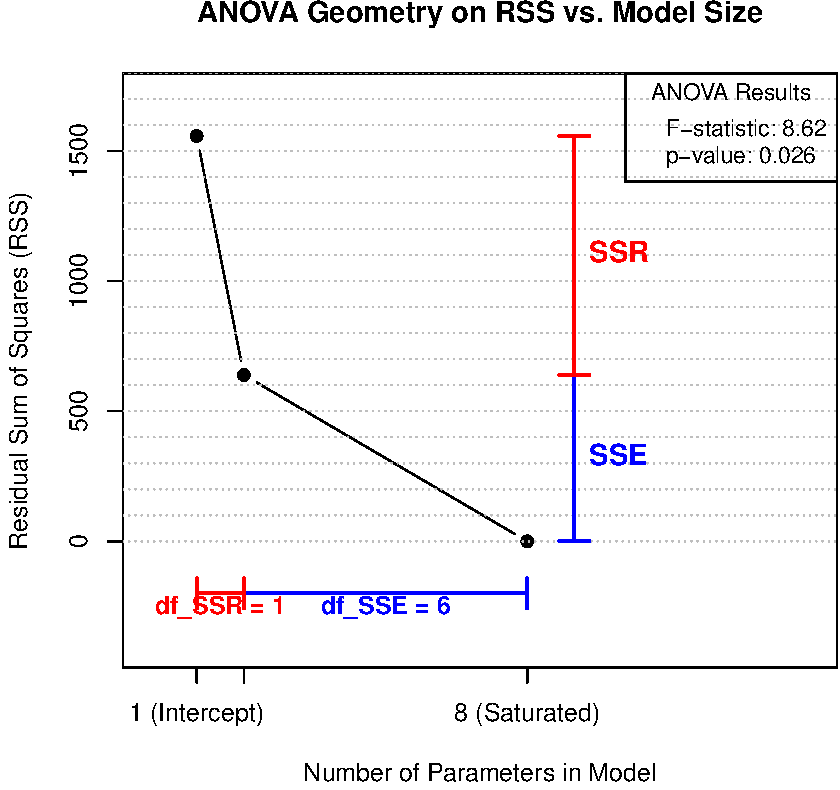
\includegraphics[keepaspectratio]{unit2-slr/slr_files/figure-pdf/unnamed-chunk-10-1.pdf}}

\subsection{\texorpdfstring{\(R^2\), \(F\) and a compact ANOVA
table}{R\^{}2, F and a compact ANOVA table}}\label{r2-f-and-a-compact-anova-table}

\begin{Shaded}
\begin{Highlighting}[]
\NormalTok{R2 }\OtherTok{\textless{}{-}}\NormalTok{ SSR }\SpecialCharTok{/}\NormalTok{ SST; R2}
\end{Highlighting}
\end{Shaded}

\begin{verbatim}
[1] 0.5897229
\end{verbatim}

\begin{Shaded}
\begin{Highlighting}[]
\NormalTok{f  }\OtherTok{\textless{}{-}}\NormalTok{ (SSR}\SpecialCharTok{/}\DecValTok{1}\NormalTok{) }\SpecialCharTok{/}\NormalTok{ (SSE}\SpecialCharTok{/}\NormalTok{(n}\DecValTok{{-}2}\NormalTok{)); f}
\end{Highlighting}
\end{Shaded}

\begin{verbatim}
[1] 8.624264
\end{verbatim}

\begin{Shaded}
\begin{Highlighting}[]
\NormalTok{pvf }\OtherTok{\textless{}{-}} \FunctionTok{pf}\NormalTok{(f, }\AttributeTok{df1 =} \DecValTok{1}\NormalTok{, }\AttributeTok{df2 =}\NormalTok{ n}\DecValTok{{-}2}\NormalTok{, }\AttributeTok{lower.tail =} \ConstantTok{FALSE}\NormalTok{); pvf}
\end{Highlighting}
\end{Shaded}

\begin{verbatim}
[1] 0.0260588
\end{verbatim}

\begin{Shaded}
\begin{Highlighting}[]
\NormalTok{Ftable }\OtherTok{\textless{}{-}} \FunctionTok{data.frame}\NormalTok{(}
  \AttributeTok{Source =} \FunctionTok{c}\NormalTok{(}\StringTok{"Regression"}\NormalTok{, }\StringTok{"Error"}\NormalTok{),}
  \AttributeTok{df     =} \FunctionTok{c}\NormalTok{(}\DecValTok{1}\NormalTok{, n }\SpecialCharTok{{-}} \DecValTok{2}\NormalTok{),}
  \AttributeTok{SS     =} \FunctionTok{c}\NormalTok{(SSR, SSE),}
  \AttributeTok{MS     =} \FunctionTok{c}\NormalTok{(SSR}\SpecialCharTok{/}\DecValTok{1}\NormalTok{, SSE}\SpecialCharTok{/}\NormalTok{(n}\DecValTok{{-}2}\NormalTok{)),}
  \AttributeTok{F      =} \FunctionTok{c}\NormalTok{(f, }\ConstantTok{NA}\NormalTok{),}
  \AttributeTok{pvalue =} \FunctionTok{c}\NormalTok{(pvf, }\ConstantTok{NA}\NormalTok{),}
  \AttributeTok{R2part =} \FunctionTok{c}\NormalTok{(SSR, SSE) }\SpecialCharTok{/}\NormalTok{ SST}
\NormalTok{)}
\NormalTok{Ftable}
\end{Highlighting}
\end{Shaded}

\begin{verbatim}
      Source df       SS       MS        F    pvalue    R2part
1 Regression  1 918.4935 918.4935 8.624264 0.0260588 0.5897229
2      Error  6 639.0065 106.5011       NA        NA 0.4102771
\end{verbatim}

A call to \texttt{anova()} reproduces the same test:

\begin{Shaded}
\begin{Highlighting}[]
\FunctionTok{anova}\NormalTok{(fit.issu)}
\end{Highlighting}
\end{Shaded}

\begin{verbatim}
Analysis of Variance Table

Response: y
          Df Sum Sq Mean Sq F value  Pr(>F)  
x          1 918.49  918.49  8.6243 0.02606 *
Residuals  6 639.01  106.50                  
---
Signif. codes:  0 '***' 0.001 '**' 0.01 '*' 0.05 '.' 0.1 ' ' 1
\end{verbatim}

\subsection{Sampling distributions via
animation}\label{sampling-distributions-via-animation}

Under \(H_0:\beta_1=0\), \(F\) follows \(F_{1,n-2}\). Under \(H_A\), the
distribution shifts right (noncentral \(F\)).

\subsubsection{\texorpdfstring{Null world (\(H_0\)
true)}{Null world (H\_0 true)}}\label{null-world-h_0-true}

\begin{Shaded}
\begin{Highlighting}[]
\NormalTok{original\_fit }\OtherTok{\textless{}{-}} \FunctionTok{lm}\NormalTok{(y }\SpecialCharTok{\textasciitilde{}}\NormalTok{ x)}
\NormalTok{intercept\_H0 }\OtherTok{\textless{}{-}} \FunctionTok{coef}\NormalTok{(original\_fit)[}\DecValTok{1}\NormalTok{]}
\NormalTok{model\_sigma  }\OtherTok{\textless{}{-}} \FunctionTok{sigma}\NormalTok{(original\_fit)}

\ControlFlowTok{for}\NormalTok{ (iter }\ControlFlowTok{in} \DecValTok{1}\SpecialCharTok{:}\DecValTok{50}\NormalTok{) \{}
\NormalTok{  sim.y }\OtherTok{\textless{}{-}}\NormalTok{ intercept\_H0 }\SpecialCharTok{+} \FunctionTok{rnorm}\NormalTok{(n, }\DecValTok{0}\NormalTok{, model\_sigma)}

  \FunctionTok{par}\NormalTok{(}\AttributeTok{mfrow =} \FunctionTok{c}\NormalTok{(}\DecValTok{1}\NormalTok{,}\DecValTok{2}\NormalTok{))}
\NormalTok{  fit.sim.y }\OtherTok{\textless{}{-}} \FunctionTok{lm}\NormalTok{(sim.y }\SpecialCharTok{\textasciitilde{}}\NormalTok{ x)}
  \FunctionTok{plot}\NormalTok{(sim.y }\SpecialCharTok{\textasciitilde{}}\NormalTok{ x, }\AttributeTok{ylim =} \FunctionTok{c}\NormalTok{(}\DecValTok{0}\NormalTok{,}\DecValTok{100}\NormalTok{), }\AttributeTok{main =} \StringTok{"Data under H0 (slope = 0)"}\NormalTok{)}
  \FunctionTok{abline}\NormalTok{(fit.sim.y, }\AttributeTok{col =} \StringTok{"red"}\NormalTok{, }\AttributeTok{lwd =} \DecValTok{2}\NormalTok{)}
  \FunctionTok{abline}\NormalTok{(}\AttributeTok{h =} \FunctionTok{mean}\NormalTok{(sim.y), }\AttributeTok{col =} \StringTok{"blue"}\NormalTok{)}

\NormalTok{  a }\OtherTok{\textless{}{-}} \FunctionTok{anova}\NormalTok{(fit.sim.y)}
\NormalTok{  ss }\OtherTok{\textless{}{-}}\NormalTok{ a}\SpecialCharTok{$}\StringTok{\textasciigrave{}}\AttributeTok{Sum Sq}\StringTok{\textasciigrave{}}\NormalTok{; rss }\OtherTok{\textless{}{-}} \FunctionTok{rev}\NormalTok{(}\FunctionTok{cumsum}\NormalTok{(}\FunctionTok{c}\NormalTok{(}\DecValTok{0}\NormalTok{, }\FunctionTok{rev}\NormalTok{(ss))))}
\NormalTok{  num.par }\OtherTok{\textless{}{-}} \FunctionTok{cumsum}\NormalTok{(}\FunctionTok{c}\NormalTok{(}\DecValTok{1}\NormalTok{, a}\SpecialCharTok{$}\NormalTok{Df))}
  \FunctionTok{plot}\NormalTok{(rss }\SpecialCharTok{\textasciitilde{}}\NormalTok{ num.par, }\AttributeTok{xlab =} \StringTok{"Number of Parameters"}\NormalTok{, }\AttributeTok{ylab =} \StringTok{"RSS"}\NormalTok{, }\AttributeTok{type =} \StringTok{"b"}\NormalTok{)}
  \FunctionTok{abline}\NormalTok{(}\AttributeTok{v =} \DecValTok{1}\SpecialCharTok{:}\DecValTok{25}\NormalTok{, }\AttributeTok{h =}\NormalTok{ (}\DecValTok{0}\SpecialCharTok{:}\DecValTok{50}\NormalTok{)}\SpecialCharTok{*}\DecValTok{100}\NormalTok{, }\AttributeTok{lty =} \DecValTok{3}\NormalTok{, }\AttributeTok{col =} \StringTok{"grey"}\NormalTok{)}

\NormalTok{  f\_value }\OtherTok{\textless{}{-}}\NormalTok{ a}\SpecialCharTok{$}\StringTok{"F value"}\NormalTok{[}\DecValTok{1}\NormalTok{]}
\NormalTok{  p\_value }\OtherTok{\textless{}{-}}\NormalTok{ a}\SpecialCharTok{$}\StringTok{"Pr(\textgreater{}F)"}\NormalTok{[}\DecValTok{1}\NormalTok{]}
  \FunctionTok{legend}\NormalTok{(}\StringTok{"topright"}\NormalTok{,}
         \AttributeTok{legend =} \FunctionTok{c}\NormalTok{(}\FunctionTok{sprintf}\NormalTok{(}\StringTok{"F: \%.2f"}\NormalTok{, f\_value),}
                    \FunctionTok{sprintf}\NormalTok{(}\StringTok{"p: \%.3f"}\NormalTok{, p\_value)),}
         \AttributeTok{title =} \StringTok{"ANOVA"}\NormalTok{, }\AttributeTok{bty =} \StringTok{"o"}\NormalTok{, }\AttributeTok{cex =} \FloatTok{0.9}\NormalTok{)}
\NormalTok{\}}
\end{Highlighting}
\end{Shaded}

\animategraphics[,controls,loop]{1}{slr_files/figure-pdf/unnamed-chunk-13-}{1}{50}

\subsubsection{\texorpdfstring{Alternative world (\(H_1\)
true)}{Alternative world (H\_1 true)}}\label{alternative-world-h_1-true}

\begin{Shaded}
\begin{Highlighting}[]
\NormalTok{original\_fit }\OtherTok{\textless{}{-}} \FunctionTok{lm}\NormalTok{(y }\SpecialCharTok{\textasciitilde{}}\NormalTok{ x)}
\NormalTok{intercept\_HA }\OtherTok{\textless{}{-}} \FunctionTok{coef}\NormalTok{(original\_fit)[}\DecValTok{1}\NormalTok{]}
\NormalTok{model\_sigma  }\OtherTok{\textless{}{-}} \FunctionTok{sigma}\NormalTok{(original\_fit)}
\NormalTok{slope\_HA     }\OtherTok{\textless{}{-}} \SpecialCharTok{{-}}\DecValTok{2}  \CommentTok{\# pick a non{-}zero slope}

\ControlFlowTok{for}\NormalTok{ (iter }\ControlFlowTok{in} \DecValTok{1}\SpecialCharTok{:}\DecValTok{50}\NormalTok{) \{}
\NormalTok{  mean\_y }\OtherTok{\textless{}{-}}\NormalTok{ intercept\_HA }\SpecialCharTok{+}\NormalTok{ slope\_HA }\SpecialCharTok{*}\NormalTok{ x}
\NormalTok{  sim.y  }\OtherTok{\textless{}{-}}\NormalTok{ mean\_y }\SpecialCharTok{+} \FunctionTok{rnorm}\NormalTok{(n, }\DecValTok{0}\NormalTok{, model\_sigma)}

  \FunctionTok{par}\NormalTok{(}\AttributeTok{mfrow =} \FunctionTok{c}\NormalTok{(}\DecValTok{1}\NormalTok{,}\DecValTok{2}\NormalTok{))}
\NormalTok{  fit.sim.y }\OtherTok{\textless{}{-}} \FunctionTok{lm}\NormalTok{(sim.y }\SpecialCharTok{\textasciitilde{}}\NormalTok{ x)}
  \FunctionTok{plot}\NormalTok{(sim.y }\SpecialCharTok{\textasciitilde{}}\NormalTok{ x, }\AttributeTok{ylim =} \FunctionTok{c}\NormalTok{(}\DecValTok{0}\NormalTok{,}\DecValTok{80}\NormalTok{), }\AttributeTok{main =} \StringTok{"Data under HA (slope = {-}2)"}\NormalTok{)}
  \FunctionTok{abline}\NormalTok{(fit.sim.y, }\AttributeTok{col =} \StringTok{"red"}\NormalTok{, }\AttributeTok{lwd =} \DecValTok{2}\NormalTok{)}
  \FunctionTok{abline}\NormalTok{(}\AttributeTok{h =} \FunctionTok{mean}\NormalTok{(sim.y), }\AttributeTok{col =} \StringTok{"blue"}\NormalTok{)}

\NormalTok{  a }\OtherTok{\textless{}{-}} \FunctionTok{anova}\NormalTok{(fit.sim.y)}
\NormalTok{  ss }\OtherTok{\textless{}{-}}\NormalTok{ a}\SpecialCharTok{$}\StringTok{\textasciigrave{}}\AttributeTok{Sum Sq}\StringTok{\textasciigrave{}}\NormalTok{; rss }\OtherTok{\textless{}{-}} \FunctionTok{rev}\NormalTok{(}\FunctionTok{cumsum}\NormalTok{(}\FunctionTok{c}\NormalTok{(}\DecValTok{0}\NormalTok{, }\FunctionTok{rev}\NormalTok{(ss))))}
\NormalTok{  num.par }\OtherTok{\textless{}{-}} \FunctionTok{cumsum}\NormalTok{(}\FunctionTok{c}\NormalTok{(}\DecValTok{1}\NormalTok{, a}\SpecialCharTok{$}\NormalTok{Df))}
  \FunctionTok{plot}\NormalTok{(rss }\SpecialCharTok{\textasciitilde{}}\NormalTok{ num.par, }\AttributeTok{xlab =} \StringTok{"Number of Parameters"}\NormalTok{, }\AttributeTok{ylab =} \StringTok{"RSS"}\NormalTok{, }\AttributeTok{type =} \StringTok{"b"}\NormalTok{)}
  \FunctionTok{abline}\NormalTok{(}\AttributeTok{v =} \DecValTok{1}\SpecialCharTok{:}\DecValTok{25}\NormalTok{, }\AttributeTok{h =}\NormalTok{ (}\DecValTok{0}\SpecialCharTok{:}\DecValTok{50}\NormalTok{)}\SpecialCharTok{*}\DecValTok{100}\NormalTok{, }\AttributeTok{lty =} \DecValTok{3}\NormalTok{, }\AttributeTok{col =} \StringTok{"grey"}\NormalTok{)}

\NormalTok{  f\_value }\OtherTok{\textless{}{-}}\NormalTok{ a}\SpecialCharTok{$}\StringTok{"F value"}\NormalTok{[}\DecValTok{1}\NormalTok{]}
\NormalTok{  p\_value }\OtherTok{\textless{}{-}}\NormalTok{ a}\SpecialCharTok{$}\StringTok{"Pr(\textgreater{}F)"}\NormalTok{[}\DecValTok{1}\NormalTok{]}
  \FunctionTok{legend}\NormalTok{(}\StringTok{"topright"}\NormalTok{,}
         \AttributeTok{legend =} \FunctionTok{c}\NormalTok{(}\FunctionTok{sprintf}\NormalTok{(}\StringTok{"F: \%.2f"}\NormalTok{, f\_value),}
                    \FunctionTok{sprintf}\NormalTok{(}\StringTok{"p: \%.3e"}\NormalTok{, p\_value)),}
         \AttributeTok{title =} \StringTok{"ANOVA"}\NormalTok{, }\AttributeTok{bty =} \StringTok{"o"}\NormalTok{, }\AttributeTok{cex =} \FloatTok{0.9}\NormalTok{)}
\NormalTok{\}}
\end{Highlighting}
\end{Shaded}

\animategraphics[,controls,loop]{1}{slr_files/figure-pdf/unnamed-chunk-14-}{1}{50}

\begin{center}\rule{0.5\linewidth}{0.5pt}\end{center}

\section{Example 2: Oxygen Purity
Data}\label{example-2-oxygen-purity-data}

We model oxygen purity \(y\) as a function of hydrocarbon level \(x\)
and report both \textbf{mean response} and \textbf{prediction}
uncertainty.

\subsection{Data}\label{data}

\begin{Shaded}
\begin{Highlighting}[]
\NormalTok{x }\OtherTok{\textless{}{-}} \FunctionTok{c}\NormalTok{(}\FloatTok{0.99}\NormalTok{, }\FloatTok{1.02}\NormalTok{, }\FloatTok{1.15}\NormalTok{, }\FloatTok{1.29}\NormalTok{, }\FloatTok{1.46}\NormalTok{, }\FloatTok{1.36}\NormalTok{, }\FloatTok{0.87}\NormalTok{, }\FloatTok{1.23}\NormalTok{, }\FloatTok{1.55}\NormalTok{, }\FloatTok{1.40}\NormalTok{, }\FloatTok{1.19}\NormalTok{,}
       \FloatTok{1.15}\NormalTok{, }\FloatTok{0.98}\NormalTok{, }\FloatTok{1.01}\NormalTok{, }\FloatTok{1.11}\NormalTok{, }\FloatTok{1.20}\NormalTok{, }\FloatTok{1.26}\NormalTok{, }\FloatTok{1.32}\NormalTok{, }\FloatTok{1.43}\NormalTok{, }\FloatTok{0.95}\NormalTok{)}
\NormalTok{y }\OtherTok{\textless{}{-}} \FunctionTok{c}\NormalTok{(}\FloatTok{90.01}\NormalTok{, }\FloatTok{89.05}\NormalTok{, }\FloatTok{91.43}\NormalTok{, }\FloatTok{93.74}\NormalTok{, }\FloatTok{96.73}\NormalTok{, }\FloatTok{94.45}\NormalTok{, }\FloatTok{87.59}\NormalTok{, }\FloatTok{91.77}\NormalTok{, }\FloatTok{99.42}\NormalTok{, }\FloatTok{93.65}\NormalTok{,}
       \FloatTok{93.54}\NormalTok{, }\FloatTok{92.52}\NormalTok{, }\FloatTok{90.56}\NormalTok{, }\FloatTok{89.54}\NormalTok{, }\FloatTok{89.85}\NormalTok{, }\FloatTok{90.39}\NormalTok{, }\FloatTok{93.25}\NormalTok{, }\FloatTok{93.41}\NormalTok{, }\FloatTok{94.98}\NormalTok{, }\FloatTok{87.33}\NormalTok{)}
\NormalTok{n }\OtherTok{\textless{}{-}} \FunctionTok{length}\NormalTok{(x); n}
\end{Highlighting}
\end{Shaded}

\begin{verbatim}
[1] 20
\end{verbatim}

\begin{Shaded}
\begin{Highlighting}[]
\NormalTok{purity.data }\OtherTok{\textless{}{-}} \FunctionTok{data.frame}\NormalTok{(}\AttributeTok{x =}\NormalTok{ x, }\AttributeTok{y =}\NormalTok{ y)}
\FunctionTok{head}\NormalTok{(purity.data)}
\end{Highlighting}
\end{Shaded}

\begin{verbatim}
     x     y
1 0.99 90.01
2 1.02 89.05
3 1.15 91.43
4 1.29 93.74
5 1.46 96.73
6 1.36 94.45
\end{verbatim}

\subsection{Fit and quick summary}\label{fit-and-quick-summary}

\begin{Shaded}
\begin{Highlighting}[]
\NormalTok{fit }\OtherTok{\textless{}{-}} \FunctionTok{lm}\NormalTok{(y }\SpecialCharTok{\textasciitilde{}}\NormalTok{ x, }\AttributeTok{data =}\NormalTok{ purity.data)}
\FunctionTok{summary}\NormalTok{(fit)}
\end{Highlighting}
\end{Shaded}

\begin{verbatim}

Call:
lm(formula = y ~ x, data = purity.data)

Residuals:
     Min       1Q   Median       3Q      Max 
-1.83029 -0.73334  0.04497  0.69969  1.96809 

Coefficients:
            Estimate Std. Error t value Pr(>|t|)    
(Intercept)   74.283      1.593   46.62  < 2e-16 ***
x             14.947      1.317   11.35 1.23e-09 ***
---
Signif. codes:  0 '***' 0.001 '**' 0.01 '*' 0.05 '.' 0.1 ' ' 1

Residual standard error: 1.087 on 18 degrees of freedom
Multiple R-squared:  0.8774,    Adjusted R-squared:  0.8706 
F-statistic: 128.9 on 1 and 18 DF,  p-value: 1.227e-09
\end{verbatim}

\textbf{Interpretation.} The slope's sign gives the direction of
association; its \(t\) test (or \(F\) with 1 df) assesses evidence for a
trend. Look at \(\hat\sigma\) for noise scale and \(R^2\) for variance
explained.

\subsection{Scatter with fitted line}\label{scatter-with-fitted-line}

\begin{Shaded}
\begin{Highlighting}[]
\FunctionTok{plot}\NormalTok{(purity.data}\SpecialCharTok{$}\NormalTok{x, purity.data}\SpecialCharTok{$}\NormalTok{y,}
     \AttributeTok{xlab =} \StringTok{"Hydrocarbon level (x)"}\NormalTok{, }\AttributeTok{ylab =} \StringTok{"Purity (y)"}\NormalTok{,}
     \AttributeTok{main =} \StringTok{"Oxygen Purity vs Hydrocarbon Level"}\NormalTok{)}
\FunctionTok{abline}\NormalTok{(fit, }\AttributeTok{col =} \StringTok{"red"}\NormalTok{, }\AttributeTok{lwd =} \DecValTok{2}\NormalTok{)}
\end{Highlighting}
\end{Shaded}

\pandocbounded{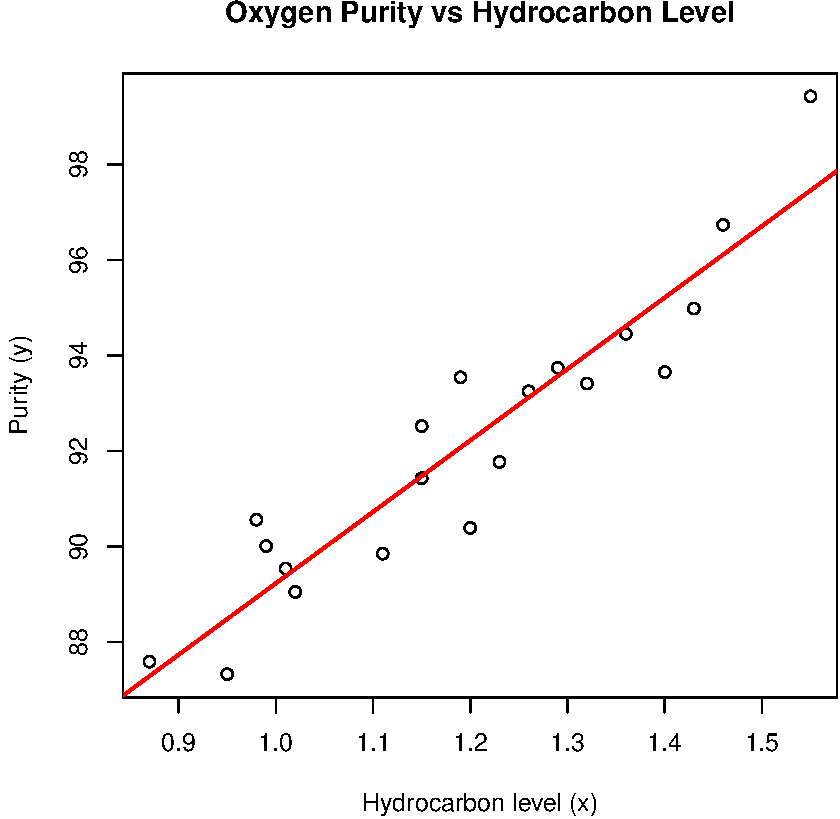
\includegraphics[keepaspectratio]{unit2-slr/slr_files/figure-pdf/plot-fit-1.pdf}}

\subsection{Coefficient CIs and ANOVA}\label{coefficient-cis-and-anova}

\begin{Shaded}
\begin{Highlighting}[]
\FunctionTok{confint}\NormalTok{(fit, }\AttributeTok{level =} \FloatTok{0.95}\NormalTok{)}
\end{Highlighting}
\end{Shaded}

\begin{verbatim}
               2.5 %   97.5 %
(Intercept) 70.93555 77.63108
x           12.18107 17.71389
\end{verbatim}

\begin{Shaded}
\begin{Highlighting}[]
\FunctionTok{anova}\NormalTok{(fit)}
\end{Highlighting}
\end{Shaded}

\begin{verbatim}
Analysis of Variance Table

Response: y
          Df Sum Sq Mean Sq F value    Pr(>F)    
x          1 152.13 152.127  128.86 1.227e-09 ***
Residuals 18  21.25   1.181                      
---
Signif. codes:  0 '***' 0.001 '**' 0.01 '*' 0.05 '.' 0.1 ' ' 1
\end{verbatim}

\subsection{Mean-response and prediction
bands}\label{mean-response-and-prediction-bands}

The \textbf{mean-response CI} narrows near \(\bar x\) and widens at the
extremes; the \textbf{prediction band} is wider by the irreducible noise
term.

\begin{Shaded}
\begin{Highlighting}[]
\NormalTok{x0 }\OtherTok{\textless{}{-}} \FunctionTok{seq}\NormalTok{(}\FunctionTok{min}\NormalTok{(purity.data}\SpecialCharTok{$}\NormalTok{x), }\FunctionTok{max}\NormalTok{(purity.data}\SpecialCharTok{$}\NormalTok{x), }\AttributeTok{length =} \DecValTok{50}\NormalTok{)}
\NormalTok{newdata }\OtherTok{\textless{}{-}} \FunctionTok{data.frame}\NormalTok{(}\AttributeTok{x =}\NormalTok{ x0)}

\NormalTok{est.mean }\OtherTok{\textless{}{-}} \FunctionTok{predict}\NormalTok{(fit, }\AttributeTok{newdata =}\NormalTok{ newdata, }\AttributeTok{interval =} \StringTok{"confidence"}\NormalTok{, }\AttributeTok{level =} \FloatTok{0.95}\NormalTok{)}
\NormalTok{pred.new }\OtherTok{\textless{}{-}} \FunctionTok{predict}\NormalTok{(fit, }\AttributeTok{newdata =}\NormalTok{ newdata, }\AttributeTok{interval =} \StringTok{"prediction"}\NormalTok{, }\AttributeTok{level =} \FloatTok{0.95}\NormalTok{)}
\end{Highlighting}
\end{Shaded}

\begin{Shaded}
\begin{Highlighting}[]
\FunctionTok{plot}\NormalTok{(purity.data}\SpecialCharTok{$}\NormalTok{x, purity.data}\SpecialCharTok{$}\NormalTok{y,}
     \AttributeTok{xlab =} \StringTok{"Hydrocarbon level (x)"}\NormalTok{, }\AttributeTok{ylab =} \StringTok{"Purity (y)"}\NormalTok{,}
     \AttributeTok{main =} \StringTok{"Regression Line with Confidence and Prediction Bands"}\NormalTok{)}
\FunctionTok{abline}\NormalTok{(fit)}
\FunctionTok{matlines}\NormalTok{(x0, est.mean[, }\DecValTok{2}\SpecialCharTok{:}\DecValTok{3}\NormalTok{], }\AttributeTok{col =} \StringTok{"blue"}\NormalTok{, }\AttributeTok{lty =} \DecValTok{2}\NormalTok{, }\AttributeTok{lwd =} \DecValTok{2}\NormalTok{)}
\FunctionTok{matlines}\NormalTok{(x0, pred.new[, }\DecValTok{2}\SpecialCharTok{:}\DecValTok{3}\NormalTok{], }\AttributeTok{col =} \StringTok{"red"}\NormalTok{,  }\AttributeTok{lty =} \DecValTok{3}\NormalTok{, }\AttributeTok{lwd =} \DecValTok{2}\NormalTok{)}
\FunctionTok{legend}\NormalTok{(}\StringTok{"topleft"}\NormalTok{, }\FunctionTok{c}\NormalTok{(}\StringTok{"Confidence Bands (mean)"}\NormalTok{, }\StringTok{"Prediction Bands (new y)"}\NormalTok{),}
       \AttributeTok{col =} \FunctionTok{c}\NormalTok{(}\StringTok{"blue"}\NormalTok{, }\StringTok{"red"}\NormalTok{), }\AttributeTok{lty =} \DecValTok{2}\SpecialCharTok{:}\DecValTok{3}\NormalTok{, }\AttributeTok{bty =} \StringTok{"n"}\NormalTok{)}
\end{Highlighting}
\end{Shaded}

\pandocbounded{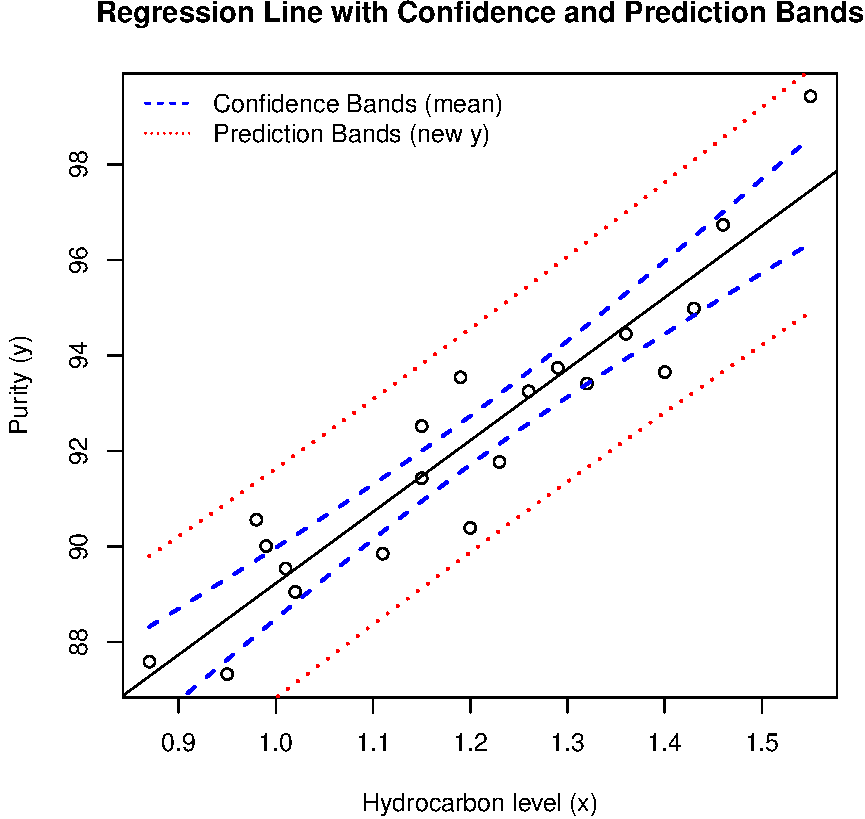
\includegraphics[keepaspectratio]{unit2-slr/slr_files/figure-pdf/plot-bands-1.pdf}}

\subsection{Residual diagnostics (assumptions
check)}\label{residual-diagnostics-assumptions-check}

We look for \textbf{no pattern} in residuals vs.~fits and
\textbf{approximate straightness} in the Q--Q plot.

\begin{Shaded}
\begin{Highlighting}[]
\NormalTok{pred }\OtherTok{\textless{}{-}} \FunctionTok{fitted.values}\NormalTok{(fit)}
\NormalTok{e }\OtherTok{\textless{}{-}} \FunctionTok{resid}\NormalTok{(fit)}
\NormalTok{d }\OtherTok{\textless{}{-}}\NormalTok{ e }\SpecialCharTok{/} \FunctionTok{summary}\NormalTok{(fit)}\SpecialCharTok{$}\NormalTok{sigma}

\FunctionTok{par}\NormalTok{(}\AttributeTok{mfrow =} \FunctionTok{c}\NormalTok{(}\DecValTok{2}\NormalTok{,}\DecValTok{2}\NormalTok{))}
\FunctionTok{plot}\NormalTok{(purity.data}\SpecialCharTok{$}\NormalTok{x, purity.data}\SpecialCharTok{$}\NormalTok{y, }\AttributeTok{xlab =} \StringTok{"x"}\NormalTok{, }\AttributeTok{ylab =} \StringTok{"y"}\NormalTok{); }\FunctionTok{abline}\NormalTok{(fit)}
\FunctionTok{qqnorm}\NormalTok{(d, }\AttributeTok{main =} \StringTok{"Normal Q–Q"}\NormalTok{); }\FunctionTok{qqline}\NormalTok{(d)}
\FunctionTok{plot}\NormalTok{(pred, d, }\AttributeTok{xlab =} \StringTok{"Fitted"}\NormalTok{, }\AttributeTok{ylab =} \StringTok{"Std. residuals"}\NormalTok{, }\AttributeTok{main =} \StringTok{"Residuals vs Fits"}\NormalTok{); }\FunctionTok{abline}\NormalTok{(}\AttributeTok{h =} \DecValTok{0}\NormalTok{, }\AttributeTok{lty =} \DecValTok{2}\NormalTok{)}
\FunctionTok{plot}\NormalTok{(}\DecValTok{1}\SpecialCharTok{:}\NormalTok{n, d, }\AttributeTok{xlab =} \StringTok{"Order"}\NormalTok{, }\AttributeTok{ylab =} \StringTok{"Std. residuals"}\NormalTok{, }\AttributeTok{main =} \StringTok{"Residuals vs Order"}\NormalTok{); }\FunctionTok{abline}\NormalTok{(}\AttributeTok{h =} \DecValTok{0}\NormalTok{, }\AttributeTok{lty =} \DecValTok{2}\NormalTok{)}
\end{Highlighting}
\end{Shaded}

\pandocbounded{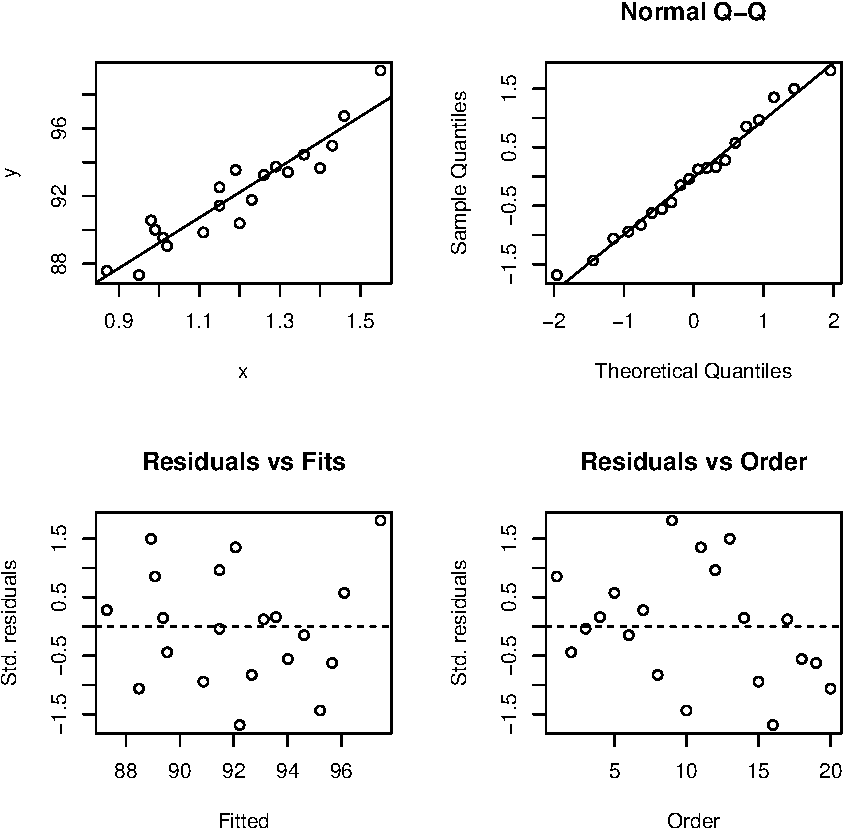
\includegraphics[keepaspectratio]{unit2-slr/slr_files/figure-pdf/residual-analysis-1.pdf}}

\begin{Shaded}
\begin{Highlighting}[]
\FunctionTok{par}\NormalTok{(}\AttributeTok{mfrow =} \FunctionTok{c}\NormalTok{(}\DecValTok{1}\NormalTok{,}\DecValTok{1}\NormalTok{))}
\end{Highlighting}
\end{Shaded}

\begin{center}\rule{0.5\linewidth}{0.5pt}\end{center}

\section{Correlation analysis (for comparison, not
causation)}\label{correlation-analysis-for-comparison-not-causation}

Correlation summarizes linear association without fitting a line or
making model assumptions.

\subsection{Data and scatter}\label{data-and-scatter}

\begin{Shaded}
\begin{Highlighting}[]
\NormalTok{strength }\OtherTok{\textless{}{-}} \FunctionTok{c}\NormalTok{(}\FloatTok{9.95}\NormalTok{,}\FloatTok{24.45}\NormalTok{,}\FloatTok{31.75}\NormalTok{,}\FloatTok{35.00}\NormalTok{,}\FloatTok{25.02}\NormalTok{,}\FloatTok{16.86}\NormalTok{,}\FloatTok{14.38}\NormalTok{,}\FloatTok{9.60}\NormalTok{,}\FloatTok{24.35}\NormalTok{,}
              \FloatTok{27.50}\NormalTok{,}\FloatTok{17.08}\NormalTok{,}\FloatTok{37.00}\NormalTok{,}\FloatTok{41.95}\NormalTok{,}\FloatTok{11.66}\NormalTok{,}\FloatTok{21.65}\NormalTok{,}\FloatTok{17.89}\NormalTok{,}\FloatTok{69.00}\NormalTok{,}\FloatTok{10.30}\NormalTok{,}
              \FloatTok{34.93}\NormalTok{,}\FloatTok{46.59}\NormalTok{,}\FloatTok{44.88}\NormalTok{,}\FloatTok{54.12}\NormalTok{,}\FloatTok{56.63}\NormalTok{,}\FloatTok{22.13}\NormalTok{,}\FloatTok{21.15}\NormalTok{)}
\NormalTok{length }\OtherTok{\textless{}{-}} \FunctionTok{c}\NormalTok{(}\DecValTok{2}\NormalTok{,}\DecValTok{8}\NormalTok{,}\DecValTok{11}\NormalTok{,}\DecValTok{10}\NormalTok{,}\DecValTok{8}\NormalTok{,}\DecValTok{4}\NormalTok{,}\DecValTok{2}\NormalTok{,}\DecValTok{2}\NormalTok{,}\DecValTok{9}\NormalTok{,}\DecValTok{8}\NormalTok{,}\DecValTok{4}\NormalTok{,}\DecValTok{11}\NormalTok{,}\DecValTok{12}\NormalTok{,}\DecValTok{2}\NormalTok{,}\DecValTok{4}\NormalTok{,}\DecValTok{4}\NormalTok{,}\DecValTok{20}\NormalTok{,}\DecValTok{1}\NormalTok{,}\DecValTok{10}\NormalTok{,}
            \DecValTok{15}\NormalTok{,}\DecValTok{15}\NormalTok{,}\DecValTok{16}\NormalTok{,}\DecValTok{17}\NormalTok{,}\DecValTok{6}\NormalTok{,}\DecValTok{5}\NormalTok{)}
\FunctionTok{plot}\NormalTok{(length, strength, }\AttributeTok{xlab =} \StringTok{"Length"}\NormalTok{, }\AttributeTok{ylab =} \StringTok{"Strength"}\NormalTok{,}
     \AttributeTok{main =} \StringTok{"Strength vs Length (scatter)"}\NormalTok{)}
\end{Highlighting}
\end{Shaded}

\pandocbounded{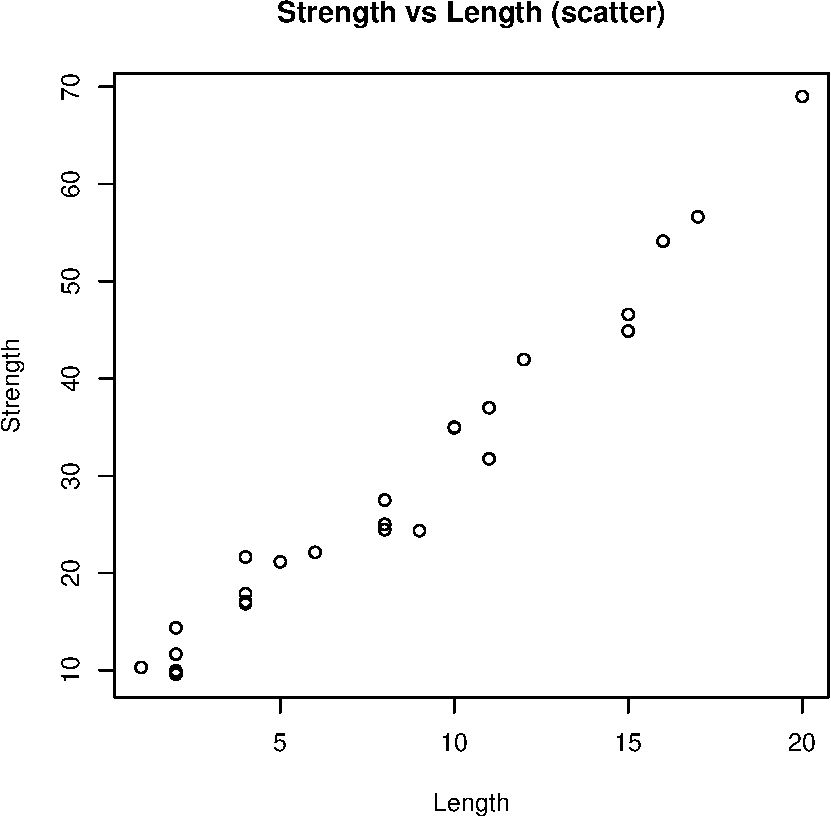
\includegraphics[keepaspectratio]{unit2-slr/slr_files/figure-pdf/correlation-data-1.pdf}}

\subsection{Pearson correlation and
test}\label{pearson-correlation-and-test}

\begin{Shaded}
\begin{Highlighting}[]
\FunctionTok{cor}\NormalTok{(strength, length)}
\end{Highlighting}
\end{Shaded}

\begin{verbatim}
[1] 0.9818118
\end{verbatim}

\begin{Shaded}
\begin{Highlighting}[]
\FunctionTok{cor.test}\NormalTok{(strength, length)}
\end{Highlighting}
\end{Shaded}

\begin{verbatim}

    Pearson's product-moment correlation

data:  strength and length
t = 24.801, df = 23, p-value < 2.2e-16
alternative hypothesis: true correlation is not equal to 0
95 percent confidence interval:
 0.9585414 0.9920735
sample estimates:
      cor 
0.9818118 
\end{verbatim}

\textbf{Note.} A large \(|r|\) and small \(p\) indicate linear
association; regression further quantifies the slope and supports
prediction, with diagnostics to check assumptions.

\begin{center}\rule{0.5\linewidth}{0.5pt}\end{center}

\section{What to report (checklist)}\label{what-to-report-checklist}

\begin{itemize}
\tightlist
\item
  Estimated line \(\hat y=\hat\beta_0+\hat\beta_1 x\) with units.
\item
  \(t\)/\(F\) test for slope, \(p\)-value and CI for \(\beta_1\).
\item
  \(R^2\) and \(\hat\sigma\) (RMSE) for fit quality.
\item
  Mean-response and prediction intervals at substantively relevant
  \(x_0\).
\item
  Residual diagnostics and any remedies (transformations, robust
  methods) if needed.
\end{itemize}

\section{Multiple Linear Regression}\label{multiple-linear-regression}

\section{An Example: Wire Bond Strength
Dataset}\label{an-example-wire-bond-strength-dataset}

\subsection{Loading Data and
Visualization}\label{loading-data-and-visualization}

\textbf{Note:} You must change the file paths in the \texttt{read.csv()}
functions below to match the location of the files on your computer (for
example
\texttt{C:\textbackslash{}\textbackslash{}Users\textbackslash{}\textbackslash{}\textless{}YourUsername\textgreater{}\textbackslash{}\textbackslash{}Documents}
on Windows).

\begin{Shaded}
\begin{Highlighting}[]
\CommentTok{\# Read data. Change the path as necessary.}
\CommentTok{\# Example: bond.data \textless{}{-} read.csv("wire{-}bond.csv")}
\NormalTok{bond.data }\OtherTok{\textless{}{-}} \FunctionTok{read.csv}\NormalTok{(}\StringTok{"wire{-}bond.csv"}\NormalTok{)}

\CommentTok{\# This will now be automatically rendered as a paged table}
\NormalTok{bond.data}
\end{Highlighting}
\end{Shaded}

\begin{verbatim}
   strength length height
1      9.95      2     50
2     24.45      8    110
3     31.75     11    120
4     35.00     10    550
5     25.02      8    295
6     16.86      4    200
7     14.38      2    375
8      9.60      2     52
9     24.35      9    100
10    27.50      8    300
11    17.08      4    412
12    37.00     11    400
13    41.95     12    500
14    11.66      2    360
15    21.65      4    205
16    17.89      4    400
17    69.00     20    600
18    10.30      1    585
19    34.93     10    540
20    46.59     15    250
21    44.88     15    290
22    54.12     16    510
23    56.63     17    590
24    22.13      6    100
25    21.15      5    400
\end{verbatim}

\textbf{2D Visualization}

\begin{Shaded}
\begin{Highlighting}[]
\FunctionTok{par}\NormalTok{(}\AttributeTok{mfrow =} \FunctionTok{c}\NormalTok{(}\DecValTok{1}\NormalTok{, }\DecValTok{3}\NormalTok{), }\AttributeTok{mar =} \FunctionTok{c}\NormalTok{(}\DecValTok{5}\NormalTok{, }\DecValTok{4}\NormalTok{, }\DecValTok{2}\NormalTok{, }\DecValTok{1}\NormalTok{))}

\CommentTok{\# 1) length vs strength}
\NormalTok{i1 }\OtherTok{\textless{}{-}} \FunctionTok{which}\NormalTok{(}\SpecialCharTok{!}\FunctionTok{is.na}\NormalTok{(bond.data}\SpecialCharTok{$}\NormalTok{length) }\SpecialCharTok{\&} \SpecialCharTok{!}\FunctionTok{is.na}\NormalTok{(bond.data}\SpecialCharTok{$}\NormalTok{strength))}
\FunctionTok{plot}\NormalTok{(bond.data}\SpecialCharTok{$}\NormalTok{length[i1], bond.data}\SpecialCharTok{$}\NormalTok{strength[i1],}
     \AttributeTok{xlab =} \StringTok{"Wire Length"}\NormalTok{, }\AttributeTok{ylab =} \StringTok{"Pull strength"}\NormalTok{, }\AttributeTok{pch =} \DecValTok{19}\NormalTok{)}
\FunctionTok{text}\NormalTok{(bond.data}\SpecialCharTok{$}\NormalTok{length[i1], bond.data}\SpecialCharTok{$}\NormalTok{strength[i1],}
     \AttributeTok{labels =}\NormalTok{ i1, }\AttributeTok{pos =} \DecValTok{1}\NormalTok{, }\AttributeTok{offset =} \FloatTok{0.4}\NormalTok{, }\AttributeTok{cex =} \FloatTok{0.75}\NormalTok{)}

\CommentTok{\# 2) height vs strength}
\NormalTok{i2 }\OtherTok{\textless{}{-}} \FunctionTok{which}\NormalTok{(}\SpecialCharTok{!}\FunctionTok{is.na}\NormalTok{(bond.data}\SpecialCharTok{$}\NormalTok{height) }\SpecialCharTok{\&} \SpecialCharTok{!}\FunctionTok{is.na}\NormalTok{(bond.data}\SpecialCharTok{$}\NormalTok{strength))}
\FunctionTok{plot}\NormalTok{(bond.data}\SpecialCharTok{$}\NormalTok{height[i2], bond.data}\SpecialCharTok{$}\NormalTok{strength[i2],}
     \AttributeTok{xlab =} \StringTok{"Die height"}\NormalTok{, }\AttributeTok{ylab =} \StringTok{"Pull strength"}\NormalTok{, }\AttributeTok{pch =} \DecValTok{19}\NormalTok{)}
\FunctionTok{text}\NormalTok{(bond.data}\SpecialCharTok{$}\NormalTok{height[i2], bond.data}\SpecialCharTok{$}\NormalTok{strength[i2],}
     \AttributeTok{labels =}\NormalTok{ i2, }\AttributeTok{pos =} \DecValTok{1}\NormalTok{, }\AttributeTok{offset =} \FloatTok{0.4}\NormalTok{, }\AttributeTok{cex =} \FloatTok{0.75}\NormalTok{)}

\CommentTok{\# 3) height vs length}
\NormalTok{i3 }\OtherTok{\textless{}{-}} \FunctionTok{which}\NormalTok{(}\SpecialCharTok{!}\FunctionTok{is.na}\NormalTok{(bond.data}\SpecialCharTok{$}\NormalTok{height) }\SpecialCharTok{\&} \SpecialCharTok{!}\FunctionTok{is.na}\NormalTok{(bond.data}\SpecialCharTok{$}\NormalTok{length))}
\FunctionTok{plot}\NormalTok{(bond.data}\SpecialCharTok{$}\NormalTok{height[i3], bond.data}\SpecialCharTok{$}\NormalTok{length[i3],}
     \AttributeTok{xlab =} \StringTok{"Die height"}\NormalTok{, }\AttributeTok{ylab =} \StringTok{"Length"}\NormalTok{, }\AttributeTok{pch =} \DecValTok{19}\NormalTok{)}
\FunctionTok{text}\NormalTok{(bond.data}\SpecialCharTok{$}\NormalTok{height[i3], bond.data}\SpecialCharTok{$}\NormalTok{length[i3],}
     \AttributeTok{labels =}\NormalTok{ i3, }\AttributeTok{pos =} \DecValTok{1}\NormalTok{, }\AttributeTok{offset =} \FloatTok{0.4}\NormalTok{, }\AttributeTok{cex =} \FloatTok{0.75}\NormalTok{)}
\end{Highlighting}
\end{Shaded}

\pandocbounded{\includegraphics[keepaspectratio]{unit3-mlr/mlr_files/figure-pdf/unnamed-chunk-3-1.pdf}}

\textbf{3D Visualize}

\begin{Shaded}
\begin{Highlighting}[]
\FunctionTok{library}\NormalTok{(scatterplot3d)}

\FunctionTok{par}\NormalTok{(}\AttributeTok{mfrow =} \FunctionTok{c}\NormalTok{(}\DecValTok{1}\NormalTok{,}\DecValTok{1}\NormalTok{))}
\NormalTok{s3d }\OtherTok{\textless{}{-}} \FunctionTok{with}\NormalTok{(bond.data, }\FunctionTok{scatterplot3d}\NormalTok{(}
  \AttributeTok{x =}\NormalTok{ length,}
  \AttributeTok{y =}\NormalTok{ height,}
  \AttributeTok{z =}\NormalTok{ strength,}
  \AttributeTok{pch =} \DecValTok{19}\NormalTok{,}
  \AttributeTok{color =} \StringTok{"steelblue"}\NormalTok{,}
  \AttributeTok{main =} \StringTok{"3D Scatterplot: Strength vs. Length and Height"}\NormalTok{,}
  \AttributeTok{xlab =} \StringTok{"Length"}\NormalTok{,}
  \AttributeTok{ylab =} \StringTok{"Height"}\NormalTok{,}
  \AttributeTok{zlab =} \StringTok{"Strength"}\NormalTok{,}
  \AttributeTok{angle =} \DecValTok{60}
\NormalTok{))}

\NormalTok{fit }\OtherTok{\textless{}{-}} \FunctionTok{lm}\NormalTok{(strength }\SpecialCharTok{\textasciitilde{}}\NormalTok{ length }\SpecialCharTok{+}\NormalTok{ height, }\AttributeTok{data =}\NormalTok{ bond.data)}
\NormalTok{s3d}\SpecialCharTok{$}\FunctionTok{plane3d}\NormalTok{(fit, }\AttributeTok{lty.box =} \StringTok{"solid"}\NormalTok{)}
\end{Highlighting}
\end{Shaded}

\pandocbounded{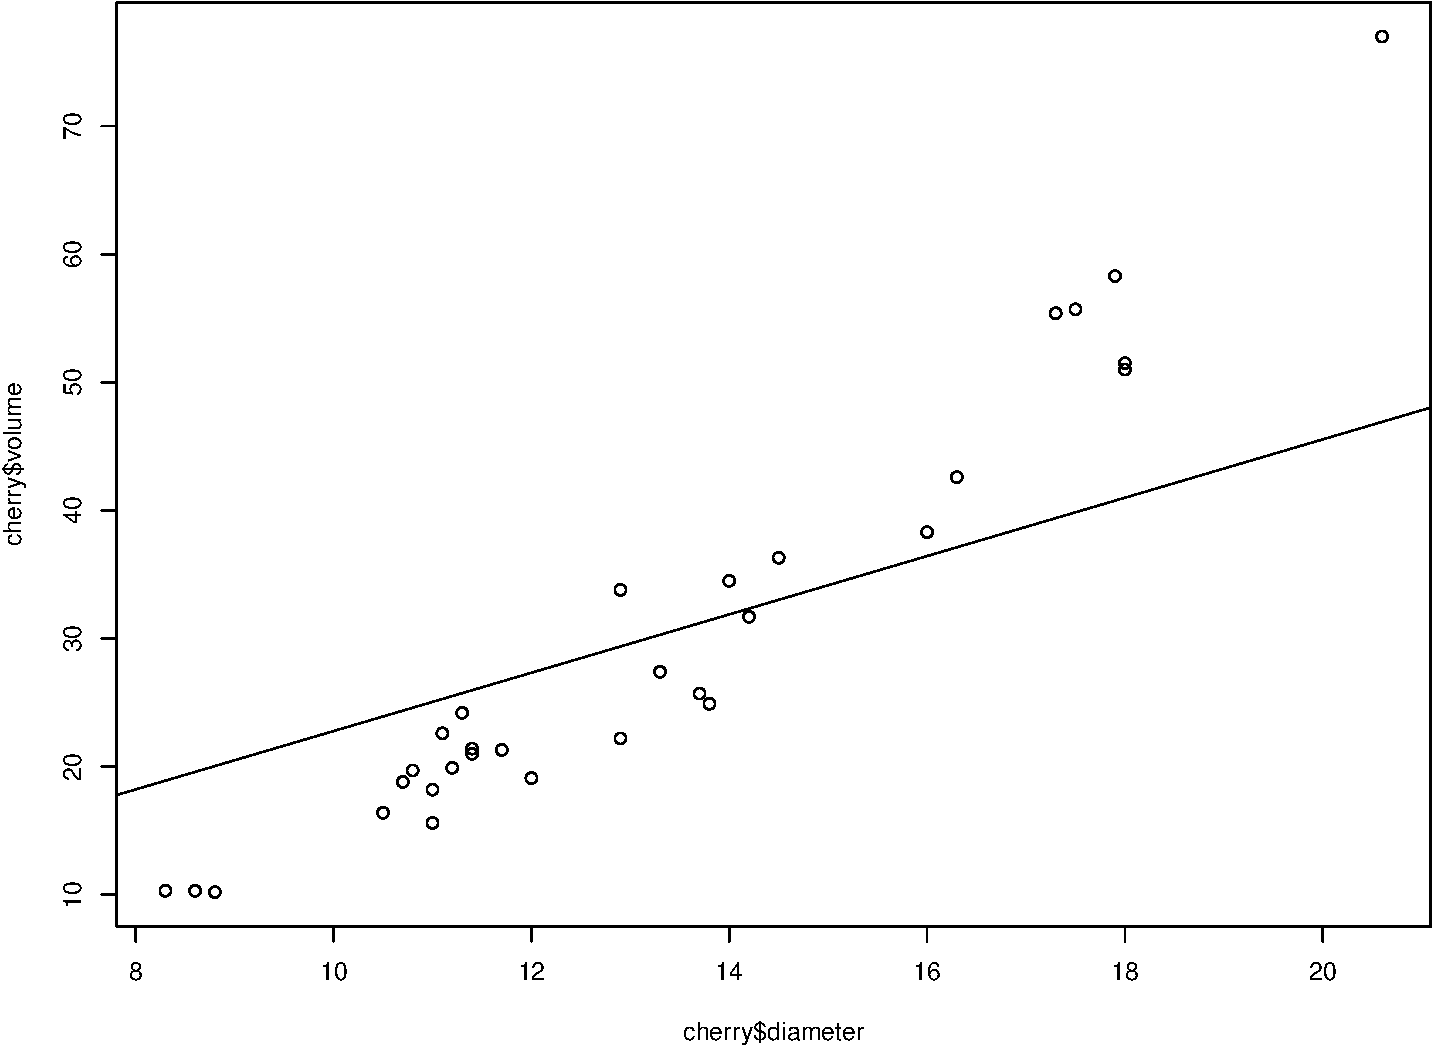
\includegraphics[keepaspectratio]{unit3-mlr/mlr_files/figure-pdf/unnamed-chunk-4-1.pdf}}

\subsection{Model Fitting and Summary}\label{model-fitting-and-summary}

We fit a multiple linear regression model with \texttt{strength} as the
response variable and \texttt{length} and \texttt{height} as predictors.

\begin{Shaded}
\begin{Highlighting}[]
\NormalTok{fit }\OtherTok{\textless{}{-}} \FunctionTok{lm}\NormalTok{(strength }\SpecialCharTok{\textasciitilde{}}\NormalTok{ length }\SpecialCharTok{+}\NormalTok{ height, }\AttributeTok{data =}\NormalTok{ bond.data)}
\FunctionTok{summary}\NormalTok{(fit)}
\end{Highlighting}
\end{Shaded}

\begin{verbatim}

Call:
lm(formula = strength ~ length + height, data = bond.data)

Residuals:
   Min     1Q Median     3Q    Max 
-3.865 -1.542 -0.362  1.196  5.841 

Coefficients:
            Estimate Std. Error t value Pr(>|t|)    
(Intercept) 2.263791   1.060066   2.136 0.044099 *  
length      2.744270   0.093524  29.343  < 2e-16 ***
height      0.012528   0.002798   4.477 0.000188 ***
---
Signif. codes:  0 '***' 0.001 '**' 0.01 '*' 0.05 '.' 0.1 ' ' 1

Residual standard error: 2.288 on 22 degrees of freedom
Multiple R-squared:  0.9811,    Adjusted R-squared:  0.9794 
F-statistic: 572.2 on 2 and 22 DF,  p-value: < 2.2e-16
\end{verbatim}

The summary provides the ANOVA F-test for overall significance, \(R^2\),
adjusted \(R^2\), and t-tests for individual coefficients.

\subsection{Confidence Intervals and Model
Components}\label{confidence-intervals-and-model-components}

\begin{Shaded}
\begin{Highlighting}[]
\CommentTok{\# Confidence intervals}
\FunctionTok{confint}\NormalTok{(fit)}
\end{Highlighting}
\end{Shaded}

\begin{verbatim}
                  2.5 %     97.5 %
(Intercept) 0.065348613 4.46223426
length      2.550313061 2.93822623
height      0.006724246 0.01833138
\end{verbatim}

\begin{Shaded}
\begin{Highlighting}[]
\CommentTok{\# Fitted values and residuals}
\NormalTok{pred }\OtherTok{\textless{}{-}} \FunctionTok{fitted.values}\NormalTok{(fit)}
\NormalTok{e }\OtherTok{\textless{}{-}} \FunctionTok{resid}\NormalTok{(fit)}
\FunctionTok{data.frame}\NormalTok{(}\AttributeTok{y =}\NormalTok{ bond.data}\SpecialCharTok{$}\NormalTok{strength, }\AttributeTok{y.hat =}\NormalTok{ pred, }\AttributeTok{e =}\NormalTok{ e)}
\end{Highlighting}
\end{Shaded}

\begin{verbatim}
       y     y.hat           e
1   9.95  8.378721  1.57127871
2  24.45 25.596008 -1.14600783
3  31.75 33.954095 -2.20409488
4  35.00 36.596784 -1.59678413
5  25.02 27.913653 -2.89365294
6  16.86 15.746432  1.11356772
7  14.38 12.450260  1.92974001
8   9.60  8.403777  1.19622309
9  24.35 28.214999 -3.86499936
10 27.50 27.976292 -0.47629200
11 17.08 18.402328 -1.32232830
12 37.00 37.461882 -0.46188206
13 41.95 41.458933  0.49106715
14 11.66 12.262343 -0.60234282
15 21.65 15.809071  5.84092866
16 17.89 18.251995 -0.36199456
17 69.00 64.665871  4.33412887
18 10.30 12.336831 -2.03683074
19 34.93 36.471506 -1.54150602
20 46.59 46.559789  0.03021107
21 44.88 47.060901 -2.18090138
22 54.12 52.561290  1.55871047
23 56.63 56.307784  0.32221591
24 22.13 19.982190  2.14780957
25 21.15 20.996264  0.15373580
\end{verbatim}

\begin{Shaded}
\begin{Highlighting}[]
\CommentTok{\# Covariance matrix and standard errors}
\NormalTok{cov.mat }\OtherTok{\textless{}{-}} \FunctionTok{vcov}\NormalTok{(fit)}
\NormalTok{cov.mat}
\end{Highlighting}
\end{Shaded}

\begin{verbatim}
             (Intercept)        length        height
(Intercept)  1.123740429 -3.921612e-02 -1.781991e-03
length      -0.039216122  8.746709e-03 -9.903775e-05
height      -0.001781991 -9.903775e-05  7.831149e-06
\end{verbatim}

\begin{Shaded}
\begin{Highlighting}[]
\FunctionTok{data.frame}\NormalTok{(}\AttributeTok{std.error =} \FunctionTok{sqrt}\NormalTok{(}\FunctionTok{diag}\NormalTok{(cov.mat)))}
\end{Highlighting}
\end{Shaded}

\begin{verbatim}
              std.error
(Intercept) 1.060066238
length      0.093523844
height      0.002798419
\end{verbatim}

\section{\texorpdfstring{RSS-based Inference: F-test, and adjusted
\(R^2\)}{RSS-based Inference: F-test, and adjusted R\^{}2}}\label{rss-based-inference-f-test-and-adjusted-r2}

\textbf{The General Linear Model}

The general linear model is:

\[y = X\beta + \epsilon\]

\begin{itemize}
\tightlist
\item
  \(y\): \(n \times 1\) vector of responses
\item
  \(X\): \(n \times p\) design matrix (first column often ones)
\item
  \(\beta\): \(p \times 1\) parameter vector, where \(p=k+1\)
\item
  \(\epsilon\): \(n \times 1\) error vector
\end{itemize}

\subsection{RSS-Based Quantities}\label{rss-based-quantities}

\subsubsection{RSS-Based Quantities}\label{rss-based-quantities-1}

\begin{longtable}[]{@{}
  >{\raggedright\arraybackslash}p{(\linewidth - 16\tabcolsep) * \real{0.1111}}
  >{\raggedright\arraybackslash}p{(\linewidth - 16\tabcolsep) * \real{0.1111}}
  >{\raggedright\arraybackslash}p{(\linewidth - 16\tabcolsep) * \real{0.1111}}
  >{\centering\arraybackslash}p{(\linewidth - 16\tabcolsep) * \real{0.1111}}
  >{\raggedright\arraybackslash}p{(\linewidth - 16\tabcolsep) * \real{0.1111}}
  >{\raggedright\arraybackslash}p{(\linewidth - 16\tabcolsep) * \real{0.1111}}
  >{\raggedright\arraybackslash}p{(\linewidth - 16\tabcolsep) * \real{0.1111}}
  >{\raggedright\arraybackslash}p{(\linewidth - 16\tabcolsep) * \real{0.1111}}
  >{\raggedright\arraybackslash}p{(\linewidth - 16\tabcolsep) * \real{0.1111}}@{}}
\toprule\noalign{}
\begin{minipage}[b]{\linewidth}\raggedright
Source
\end{minipage} & \begin{minipage}[b]{\linewidth}\raggedright
Sum of Squares
\end{minipage} & \begin{minipage}[b]{\linewidth}\raggedright
\(R^2\)
\end{minipage} & \begin{minipage}[b]{\linewidth}\centering
df
\end{minipage} & \begin{minipage}[b]{\linewidth}\raggedright
Mean Squares
\end{minipage} & \begin{minipage}[b]{\linewidth}\raggedright
\(F\)
\end{minipage} & \begin{minipage}[b]{\linewidth}\raggedright
SS\(_\mathrm{adj}\)
\end{minipage} & \begin{minipage}[b]{\linewidth}\raggedright
\(\hat{\sigma}^2\)
\end{minipage} & \begin{minipage}[b]{\linewidth}\raggedright
\(R^2_{\mathrm{adj}}\)
\end{minipage} \\
\midrule\noalign{}
\endhead
\bottomrule\noalign{}
\endlastfoot
\(x^\top\beta\) &
\(\mathrm{SSR} = \displaystyle \sum_{i=1}^n (\hat y_i - \bar y)^2\) &
\(\displaystyle \frac{\mathrm{SSR}}{\mathrm{SST}}\) & \(k\) &
\(\displaystyle \mathrm{MSR} = \frac{\mathrm{SSR}}{k}\) &
\(\displaystyle \frac{\mathrm{MSR}}{\mathrm{MSE}}\) &
\(\mathrm{SSR}_{\mathrm{adj}}\) &
\(\displaystyle \hat{\sigma}^2_{x^\top\beta} = \frac{\mathrm{SSR}_{\mathrm{adj}}}{n-1}\)
&
\(\displaystyle \frac{\mathrm{SSR}_{\mathrm{adj}}}{\mathrm{SST}} = 1 - \frac{\mathrm{MSE}}{\mathrm{MST}}\) \\
\(\epsilon\) &
\(\mathrm{SSE} = \displaystyle \sum_{i=1}^n (y_i - \hat y_i)^2\) & --- &
\(n-p\) & \(\displaystyle \mathrm{MSE} = \frac{\mathrm{SSE}}{n-p}\) &
--- & \(\mathrm{SSE}\) &
\(\displaystyle \hat{\sigma}^2_{\epsilon} = \mathrm{MSE}\) & --- \\
\(y\) & \(\mathrm{SST} = \displaystyle \sum_{i=1}^n (y_i - \bar y)^2\) &
--- & \(n-1\) &
\(\displaystyle \mathrm{MST} = \frac{\mathrm{SST}}{n-1}\) & --- &
\(\mathrm{SST}\) & \(\displaystyle \hat{\sigma}^2_{y} = \mathrm{MST}\) &
--- \\
\end{longtable}

\begin{center}\rule{0.5\linewidth}{0.5pt}\end{center}

\textbf{Interpretation of the} \(\hat{\sigma}^2\) Column

The \(\hat{\sigma}^2\) column highlights how each sum of squares
corresponds to an estimated variance.\\
This view makes the adjusted coefficient of determination clear:

\[
R^2_{\mathrm{adj}} 
= 1 - \frac{\hat{\sigma}^2_\epsilon}{\hat{\sigma}^2_y}
= \frac{\hat{\sigma}^2_{x^\top\beta}}{\hat{\sigma}^2_y}.
\]

Hence, the adjusted \(R^2\) simply expresses the \textbf{proportion of
total estimated variance} attributable to the fitted model \(X\beta\)
rather than the residual noise \(\epsilon\).

\subsection{Remarks}\label{remarks}

\subsubsection{Fundamental Identities}\label{fundamental-identities}

\[
\begin{aligned}
\mathrm{SST} &= \mathrm{SSR} + \mathrm{SSE}, \\
\mathrm{MST} &= \mathrm{MSE} + \frac{\mathrm{SSR}_{\mathrm{adj}}}{n-1}.
\end{aligned}
\]

where

\[
\mathrm{SSR}_{\mathrm{adj}} = (n-1)MST-(n-p+k)\mathrm{MSE} = \mathrm{SST}-\mathrm{SSE} - k\,\mathrm{MSE} = \mathrm{SSR} - k\,\mathrm{MSE}.
\]

\begin{center}\rule{0.5\linewidth}{0.5pt}\end{center}

\subsubsection{\texorpdfstring{Difference of \(\hat{\sigma}^2\) and Mean
Squares}{Difference of \textbackslash hat\{\textbackslash sigma\}\^{}2 and Mean Squares}}\label{difference-of-hatsigma2-and-mean-squares}

The quantity \(\hat{\sigma}^2\) represents the \textbf{estimated
variance} associated with each component of the model. MSE and MST are
the estimated variances of the \(\epsilon\) and \(y\) itself. However,
the MSR, although called \textbf{Mean Square for Regression (MSR)} is
\emph{NOT} an estimate of the variance or sample variance of
\(x^\top \beta\). The name of ``mean'' here is used to indicate a
different thing. Its name ``Mean Square'' reflects that it is also an
estimate estimate of noise variance \(\sigma^2\) under
\(H_0\!:\,\beta = 0\):

\[
E[\mathrm{MSR} \mid H_0] = \sigma^2,
\qquad 
E[\mathrm{MSR} \mid H_1] > \sigma^2.
\]

Hence the F-statistic

\[
F = \frac{\mathrm{MSR}}{\mathrm{MSE}}
\] is approximately equal to 1 subject to the variability as
characterized with F-distribution with degree freedoms of \(k\) and
\(n-p\). This test is to test whether any regression coefficients are
not equal to 0.

\begin{center}\rule{0.5\linewidth}{0.5pt}\end{center}

\subsubsection{\texorpdfstring{\(\hat \sigma^2_{x^\top\beta}=\frac{\mathrm{SSR}_{\text{adj}}}{n-1}\)}{\textbackslash hat \textbackslash sigma\^{}2\_\{x\^{}\textbackslash top\textbackslash beta\}=\textbackslash frac\{\textbackslash mathrm\{SSR\}\_\{\textbackslash text\{adj\}\}\}\{n-1\}}}\label{hat-sigma2_xtopbetafracmathrmssr_textadjn-1}

\(\hat \sigma^2_{x^\top\beta}\) is an unbiased estimator of the variance
of linear signal when \(x\) is a regarded as a random variable. This can
be seen from the following equations: \[
E[\mathrm{SSR}] = k\,\sigma^2 + \beta^\top X^\top (I - J/n)\,X\,\beta,
\qquad
E[\mathrm{MSE}] = \sigma^2.
\] Hence, \[
\begin{aligned}
E[\mathrm{SSR}_{\mathrm{adj}}]
&= E[\mathrm{SSR}] - k\,E[\mathrm{MSE}] \\
&= \beta^\top X^\top (I - J/n)\,X\,\beta \\
&= \sum_{i=1}^n (\mu_i - \bar\mu)^2,
\end{aligned}
\]

where \[
\begin{aligned}
\mu_i &= x_i^\top \beta \\
\bar\mu &= \tfrac{1}{n}\sum_{i=1}^n \mu_i
\end{aligned}
\] For fixed \(X\), \(\mathrm{SSR}_{\text{adj}}/(n-1)\) equals the
\textbf{sample variance} of the true means \(\{\mu_i\}\) over the
observed design points. If the rows of \(X\) are independently sampled
with covariance matrix \(\Sigma_X\) (the random-\(X\) model), then

\[
\mathbb{E}_X\!\left[\frac{\mathrm{SSR}_{\text{adj}}}{n-1}\right]
= \beta^\top \Sigma_X \beta
= \mathrm{Var}(x^\top \beta),
\]

\subsubsection{Connection to Rao-Blackwell
Formula}\label{connection-to-rao-blackwell-formula}

The decomposition of \(\hat{\sigma}^2\) is consistent with the
\textbf{Rao--Blackwell formula} for total variance:

\[
\mathrm{Var}(y) = \mathrm{Var}\!\big(E[y \mid x]\big) + E\!\big(\mathrm{Var}[y \mid x]\big).
\]

Here,

\begin{itemize}
\tightlist
\item
  \(\mathrm{Var}\!\big(E[y \mid x]\big)\) corresponds to the
  \textbf{explained variation} due to the regression component
  \(x^\top\beta\), and\\
\item
  \(E\!\big(\mathrm{Var}[y \mid x]\big)\) corresponds to the
  \textbf{residual variation} due to \(\epsilon\).
\end{itemize}

\subsection{A Simulation Study to Understand the Distributions of
RSS}\label{a-simulation-study-to-understand-the-distributions-of-rss}

\textbf{Data Generating Model}

For \(n=30\) and \(p_{max}=20\), simulate with either
\(H_0:\beta=\mathbf 0\) or \(H_1\) where only \(\beta_1\neq 0\);
\(\epsilon_i\sim N(0,1)\).

\textbf{Sequence of Fitted Models}

\begin{longtable}[]{@{}
  >{\raggedright\arraybackslash}p{(\linewidth - 6\tabcolsep) * \real{0.2297}}
  >{\centering\arraybackslash}p{(\linewidth - 6\tabcolsep) * \real{0.2432}}
  >{\centering\arraybackslash}p{(\linewidth - 6\tabcolsep) * \real{0.2432}}
  >{\raggedright\arraybackslash}p{(\linewidth - 6\tabcolsep) * \real{0.2838}}@{}}
\toprule\noalign{}
\begin{minipage}[b]{\linewidth}\raggedright
Model Name
\end{minipage} & \begin{minipage}[b]{\linewidth}\centering
\# of Predictors (k)
\end{minipage} & \begin{minipage}[b]{\linewidth}\centering
\# of Parameters (p)
\end{minipage} & \begin{minipage}[b]{\linewidth}\raggedright
R Formula
\end{minipage} \\
\midrule\noalign{}
\endhead
\bottomrule\noalign{}
\endlastfoot
Model 0 & 0 & 1 & \texttt{y\ \textasciitilde{}\ 1} \\
Model 1 & 2 & 3 & \texttt{y\ \textasciitilde{}\ x\_1\ +\ x\_2} \\
\ldots{} & \ldots{} & \ldots{} & \ldots{} \\
Final Model & 20 & 21 &
\texttt{y\ \textasciitilde{}\ x\_1\ +\ ...\ +\ x\_20} \\
\end{longtable}

\subsubsection{\texorpdfstring{When \(H_0\) is
true}{When H\_0 is true}}\label{when-h_0-is-true}

\begin{Shaded}
\begin{Highlighting}[]
\FunctionTok{cat}\NormalTok{(}\FunctionTok{sprintf}\NormalTok{(}\StringTok{\textquotesingle{}\textless{}video controls style="width:100\%\%;height:auto;"\textgreater{}\textless{}source src="\%s" type="video/mp4"\textgreater{}\textless{}/video\textgreater{}\textquotesingle{}}\NormalTok{,}\StringTok{"rss{-}h0.mp4"}\NormalTok{))}
\end{Highlighting}
\end{Shaded}

\subsubsection{\texorpdfstring{When \(H_1\) is
true}{When H\_1 is true}}\label{when-h_1-is-true}

\begin{Shaded}
\begin{Highlighting}[]
\FunctionTok{cat}\NormalTok{(}\FunctionTok{sprintf}\NormalTok{(}\StringTok{\textquotesingle{}\textless{}video controls style="width:100\%\%;height:auto;"\textgreater{}\textless{}source src="\%s" type="video/mp4"\textgreater{}\textless{}/video\textgreater{}\textquotesingle{}}\NormalTok{,}\StringTok{"rss{-}h1.mp4"}\NormalTok{))}
\end{Highlighting}
\end{Shaded}

\subsection{Example}\label{example}

\begin{Shaded}
\begin{Highlighting}[]
\CommentTok{\# Data: Weight, height and age of children}
\NormalTok{wgt }\OtherTok{\textless{}{-}} \FunctionTok{c}\NormalTok{(}\DecValTok{64}\NormalTok{, }\DecValTok{71}\NormalTok{, }\DecValTok{53}\NormalTok{, }\DecValTok{67}\NormalTok{, }\DecValTok{55}\NormalTok{, }\DecValTok{58}\NormalTok{, }\DecValTok{77}\NormalTok{, }\DecValTok{57}\NormalTok{, }\DecValTok{56}\NormalTok{, }\DecValTok{51}\NormalTok{, }\DecValTok{76}\NormalTok{, }\DecValTok{68}\NormalTok{)}
\NormalTok{hgt }\OtherTok{\textless{}{-}} \FunctionTok{c}\NormalTok{(}\DecValTok{57}\NormalTok{, }\DecValTok{59}\NormalTok{, }\DecValTok{49}\NormalTok{, }\DecValTok{62}\NormalTok{, }\DecValTok{51}\NormalTok{, }\DecValTok{50}\NormalTok{, }\DecValTok{55}\NormalTok{, }\DecValTok{48}\NormalTok{, }\DecValTok{42}\NormalTok{, }\DecValTok{42}\NormalTok{, }\DecValTok{61}\NormalTok{, }\DecValTok{57}\NormalTok{)}
\NormalTok{age }\OtherTok{\textless{}{-}} \FunctionTok{c}\NormalTok{(}\DecValTok{8}\NormalTok{, }\DecValTok{10}\NormalTok{, }\DecValTok{6}\NormalTok{, }\DecValTok{11}\NormalTok{, }\DecValTok{8}\NormalTok{, }\DecValTok{7}\NormalTok{, }\DecValTok{10}\NormalTok{, }\DecValTok{9}\NormalTok{, }\DecValTok{10}\NormalTok{, }\DecValTok{6}\NormalTok{, }\DecValTok{12}\NormalTok{, }\DecValTok{9}\NormalTok{)}
\NormalTok{child.data }\OtherTok{\textless{}{-}} \FunctionTok{data.frame}\NormalTok{(wgt, hgt, age)}
\end{Highlighting}
\end{Shaded}

\subsubsection{Problem 1: Height then
Age}\label{problem-1-height-then-age}

\begin{Shaded}
\begin{Highlighting}[]
\NormalTok{fit\_age\_hgt }\OtherTok{\textless{}{-}} \FunctionTok{lm}\NormalTok{(wgt }\SpecialCharTok{\textasciitilde{}}\NormalTok{ hgt }\SpecialCharTok{+}\NormalTok{ age, }\AttributeTok{data =}\NormalTok{ child.data)}
\FunctionTok{summary}\NormalTok{(fit\_age\_hgt)}
\end{Highlighting}
\end{Shaded}

\begin{verbatim}

Call:
lm(formula = wgt ~ hgt + age, data = child.data)

Residuals:
    Min      1Q  Median      3Q     Max 
-6.8708 -1.7004  0.3454  1.4642 10.2336 

Coefficients:
            Estimate Std. Error t value Pr(>|t|)  
(Intercept)   6.5530    10.9448   0.599   0.5641  
hgt           0.7220     0.2608   2.768   0.0218 *
age           2.0501     0.9372   2.187   0.0565 .
---
Signif. codes:  0 '***' 0.001 '**' 0.01 '*' 0.05 '.' 0.1 ' ' 1

Residual standard error: 4.66 on 9 degrees of freedom
Multiple R-squared:   0.78, Adjusted R-squared:  0.7311 
F-statistic: 15.95 on 2 and 9 DF,  p-value: 0.001099
\end{verbatim}

\begin{Shaded}
\begin{Highlighting}[]
\NormalTok{fit\_hgt }\OtherTok{\textless{}{-}} \FunctionTok{lm}\NormalTok{(wgt }\SpecialCharTok{\textasciitilde{}}\NormalTok{ hgt, }\AttributeTok{data =}\NormalTok{ child.data)}
\FunctionTok{summary}\NormalTok{(fit\_hgt)}
\end{Highlighting}
\end{Shaded}

\begin{verbatim}

Call:
lm(formula = wgt ~ hgt, data = child.data)

Residuals:
    Min      1Q  Median      3Q     Max 
-5.8736 -3.8973 -0.4402  2.2624 11.8375 

Coefficients:
            Estimate Std. Error t value Pr(>|t|)   
(Intercept)   6.1898    12.8487   0.482  0.64035   
hgt           1.0722     0.2417   4.436  0.00126 **
---
Signif. codes:  0 '***' 0.001 '**' 0.01 '*' 0.05 '.' 0.1 ' ' 1

Residual standard error: 5.471 on 10 degrees of freedom
Multiple R-squared:  0.663, Adjusted R-squared:  0.6293 
F-statistic: 19.67 on 1 and 10 DF,  p-value: 0.001263
\end{verbatim}

\begin{Shaded}
\begin{Highlighting}[]
\FunctionTok{anova}\NormalTok{(fit\_hgt, fit\_age\_hgt)}
\end{Highlighting}
\end{Shaded}

\begin{verbatim}
Analysis of Variance Table

Model 1: wgt ~ hgt
Model 2: wgt ~ hgt + age
  Res.Df    RSS Df Sum of Sq      F  Pr(>F)  
1     10 299.33                              
2      9 195.43  1     103.9 4.7849 0.05649 .
---
Signif. codes:  0 '***' 0.001 '**' 0.01 '*' 0.05 '.' 0.1 ' ' 1
\end{verbatim}

\subsubsection{Problem 2: Age then
Height}\label{problem-2-age-then-height}

\begin{Shaded}
\begin{Highlighting}[]
\NormalTok{fit\_age }\OtherTok{\textless{}{-}} \FunctionTok{lm}\NormalTok{(wgt }\SpecialCharTok{\textasciitilde{}}\NormalTok{ age, }\AttributeTok{data =}\NormalTok{ child.data)}
\FunctionTok{summary}\NormalTok{(fit\_age)}
\end{Highlighting}
\end{Shaded}

\begin{verbatim}

Call:
lm(formula = wgt ~ age, data = child.data)

Residuals:
    Min      1Q  Median      3Q     Max 
-11.000  -3.911   1.143   4.071  10.000 

Coefficients:
            Estimate Std. Error t value Pr(>|t|)   
(Intercept)  30.5714     8.6137   3.549  0.00528 **
age           3.6429     0.9551   3.814  0.00341 **
---
Signif. codes:  0 '***' 0.001 '**' 0.01 '*' 0.05 '.' 0.1 ' ' 1

Residual standard error: 6.015 on 10 degrees of freedom
Multiple R-squared:  0.5926,    Adjusted R-squared:  0.5519 
F-statistic: 14.55 on 1 and 10 DF,  p-value: 0.003407
\end{verbatim}

\begin{Shaded}
\begin{Highlighting}[]
\NormalTok{fit\_age\_hgt }\OtherTok{\textless{}{-}} \FunctionTok{lm}\NormalTok{(wgt }\SpecialCharTok{\textasciitilde{}}\NormalTok{ age }\SpecialCharTok{+}\NormalTok{ hgt, }\AttributeTok{data =}\NormalTok{ child.data)}
\FunctionTok{summary}\NormalTok{(fit\_age\_hgt)}
\end{Highlighting}
\end{Shaded}

\begin{verbatim}

Call:
lm(formula = wgt ~ age + hgt, data = child.data)

Residuals:
    Min      1Q  Median      3Q     Max 
-6.8708 -1.7004  0.3454  1.4642 10.2336 

Coefficients:
            Estimate Std. Error t value Pr(>|t|)  
(Intercept)   6.5530    10.9448   0.599   0.5641  
age           2.0501     0.9372   2.187   0.0565 .
hgt           0.7220     0.2608   2.768   0.0218 *
---
Signif. codes:  0 '***' 0.001 '**' 0.01 '*' 0.05 '.' 0.1 ' ' 1

Residual standard error: 4.66 on 9 degrees of freedom
Multiple R-squared:   0.78, Adjusted R-squared:  0.7311 
F-statistic: 15.95 on 2 and 9 DF,  p-value: 0.001099
\end{verbatim}

\begin{Shaded}
\begin{Highlighting}[]
\FunctionTok{anova}\NormalTok{(fit\_age, fit\_age\_hgt)}
\end{Highlighting}
\end{Shaded}

\begin{verbatim}
Analysis of Variance Table

Model 1: wgt ~ age
Model 2: wgt ~ age + hgt
  Res.Df    RSS Df Sum of Sq      F  Pr(>F)  
1     10 361.86                              
2      9 195.43  1    166.43 7.6646 0.02181 *
---
Signif. codes:  0 '***' 0.001 '**' 0.01 '*' 0.05 '.' 0.1 ' ' 1
\end{verbatim}

\subsection{Relationship between t-test and partial
F-test}\label{relationship-between-t-test-and-partial-f-test}

\begin{itemize}
\tightlist
\item
  A t-test for a single coefficient is a special case of the partial
  F-test; the relationship is \(F = t^2\) for 1 df in the numerator.
\item
  The p-value from t-test (output of \emph{summary(lm())}) is the same
  as anova test for: \(H_0: \beta_j = 0\) vs \(H_1\): all covaraites
  have non-zero effects.
\end{itemize}

\section{Predictions for Mean Response and a Future
Observation}\label{predictions-for-mean-response-and-a-future-observation}

\subsection{Confidence Interval for Mean
Response}\label{confidence-interval-for-mean-response}

\begin{Shaded}
\begin{Highlighting}[]
\FunctionTok{predict}\NormalTok{(fit, }\AttributeTok{newdata =} \FunctionTok{data.frame}\NormalTok{(}\AttributeTok{length =} \DecValTok{8}\NormalTok{, }\AttributeTok{height =} \DecValTok{275}\NormalTok{),}
        \AttributeTok{interval =} \StringTok{"confidence"}\NormalTok{, }\AttributeTok{level =} \FloatTok{0.95}\NormalTok{)}
\end{Highlighting}
\end{Shaded}

\begin{verbatim}
      fit      lwr      upr
1 27.6631 26.66324 28.66296
\end{verbatim}

\subsection{Prediction Interval for a New
Observation}\label{prediction-interval-for-a-new-observation}

\begin{Shaded}
\begin{Highlighting}[]
\FunctionTok{predict}\NormalTok{(fit, }\AttributeTok{newdata =} \FunctionTok{data.frame}\NormalTok{(}\AttributeTok{length =} \DecValTok{8}\NormalTok{, }\AttributeTok{height =} \DecValTok{275}\NormalTok{),}
        \AttributeTok{interval =} \StringTok{"prediction"}\NormalTok{, }\AttributeTok{level =} \FloatTok{0.95}\NormalTok{)}
\end{Highlighting}
\end{Shaded}

\begin{verbatim}
      fit      lwr      upr
1 27.6631 22.81378 32.51241
\end{verbatim}

\section{Model Diagnostics}\label{model-diagnostics}

\subsection{Residual Calculations}\label{residual-calculations}

\begin{Shaded}
\begin{Highlighting}[]
\NormalTok{residuals\_df }\OtherTok{\textless{}{-}} \FunctionTok{data.frame}\NormalTok{(}
  \AttributeTok{hat\_values =} \FunctionTok{hatvalues}\NormalTok{(fit),}
  \AttributeTok{ordinary\_resid =} \FunctionTok{resid}\NormalTok{(fit),}
  \AttributeTok{standardized\_resid =} \FunctionTok{resid}\NormalTok{(fit) }\SpecialCharTok{/} \FunctionTok{sigma}\NormalTok{(fit),}
  \AttributeTok{studentized\_internal =} \FunctionTok{rstandard}\NormalTok{(fit),}
  \AttributeTok{studentized\_external =} \FunctionTok{rstudent}\NormalTok{(fit)}
\NormalTok{)}
\NormalTok{residuals\_df}
\end{Highlighting}
\end{Shaded}

\begin{verbatim}
   hat_values ordinary_resid standardized_resid studentized_internal
1  0.15728923     1.57127871         0.68673363           0.74808172
2  0.11164598    -1.14600783        -0.50086730          -0.53140990
3  0.14191905    -2.20409488        -0.96330846          -1.03992315
4  0.10188923    -1.59678413        -0.69788088          -0.73640435
5  0.04178381    -2.89365294        -1.26468257          -1.29196212
6  0.07486842     1.11356772         0.48668921           0.50599936
7  0.11806106     1.92974001         0.84340057           0.89807919
8  0.15608149     1.19622309         0.52281407           0.56911105
9  0.12797685    -3.86499936        -1.68921340          -1.80892479
10 0.04131672    -0.47629200        -0.20816532          -0.21260369
11 0.09253979    -1.32232830        -0.57792886          -0.60668127
12 0.05256700    -0.46188206        -0.20186740          -0.20739197
13 0.08202675     0.49106715         0.21462286           0.22400668
14 0.11291577    -0.60234282        -0.26325633          -0.27950939
15 0.07373697     5.84092866         2.55280118           2.65246601
16 0.08794942    -0.36199456        -0.15821117          -0.16566382
17 0.25934228     4.33412887         1.89424832           2.20104100
18 0.29287870    -2.03683074        -0.89020500          -1.05862725
19 0.09617553    -1.54150602        -0.67372136          -0.70866056
20 0.14726101     0.03021107         0.01320387           0.01429859
21 0.12963943    -2.18090138        -0.95317165          -1.02169558
22 0.13580052     1.55871047         0.68124063           0.73281364
23 0.18237610     0.32221591         0.14082575           0.15574183
24 0.10908869     2.14780957         0.93870874           0.99452024
25 0.07287021     0.15373580         0.06719084           0.06978142
   studentized_external
1            0.74035927
2           -0.52255660
3           -1.04194550
4           -0.72850799
5           -1.31305171
6            0.49726770
7            0.89397096
8            0.56016499
9           -1.91552083
10          -0.20792931
11          -0.59775404
12          -0.20282206
13           0.21910643
14          -0.27356920
15           3.14216850
16          -0.16195600
17           2.43521394
18          -1.06168251
19          -0.70040768
20           0.01396991
21          -1.02276424
22           0.72486668
23           0.15224503
24           0.99426154
25           0.06818458
\end{verbatim}

\subsection{Residual Plots}\label{residual-plots}

\begin{Shaded}
\begin{Highlighting}[]
\NormalTok{n }\OtherTok{\textless{}{-}} \FunctionTok{nrow}\NormalTok{(bond.data)}
\NormalTok{r }\OtherTok{\textless{}{-}} \FunctionTok{rstudent}\NormalTok{(fit) }
\NormalTok{y.hat }\OtherTok{\textless{}{-}} \FunctionTok{fitted.values}\NormalTok{(fit)}

\FunctionTok{par}\NormalTok{(}\AttributeTok{mfrow =} \FunctionTok{c}\NormalTok{(}\DecValTok{2}\NormalTok{, }\DecValTok{3}\NormalTok{))}
\FunctionTok{qqnorm}\NormalTok{(r, }\AttributeTok{main =} \StringTok{"Normal Q{-}Q Plot"}\NormalTok{); }\FunctionTok{qqline}\NormalTok{(r)}
\FunctionTok{plot}\NormalTok{(y.hat, r, }\AttributeTok{xlab =} \StringTok{"Fitted values"}\NormalTok{, }\AttributeTok{ylab =} \StringTok{"Studentized Residuals"}\NormalTok{); }\FunctionTok{abline}\NormalTok{(}\AttributeTok{h =} \DecValTok{0}\NormalTok{)}
\FunctionTok{plot}\NormalTok{(}\DecValTok{1}\SpecialCharTok{:}\NormalTok{n, r, }\AttributeTok{xlab =} \StringTok{"Observation Number"}\NormalTok{, }\AttributeTok{ylab =} \StringTok{"Studentized Residuals"}\NormalTok{); }\FunctionTok{abline}\NormalTok{(}\AttributeTok{h =} \DecValTok{0}\NormalTok{)}
\FunctionTok{plot}\NormalTok{(bond.data}\SpecialCharTok{$}\NormalTok{length, r, }\AttributeTok{xlab =} \StringTok{"Wire Length"}\NormalTok{, }\AttributeTok{ylab =} \StringTok{"Studentized Residuals"}\NormalTok{); }\FunctionTok{abline}\NormalTok{(}\AttributeTok{h =} \DecValTok{0}\NormalTok{)}
\FunctionTok{plot}\NormalTok{(bond.data}\SpecialCharTok{$}\NormalTok{height, r, }\AttributeTok{xlab =} \StringTok{"Die Height"}\NormalTok{, }\AttributeTok{ylab =} \StringTok{"Studentized Residuals"}\NormalTok{); }\FunctionTok{abline}\NormalTok{(}\AttributeTok{h =} \DecValTok{0}\NormalTok{)}
\end{Highlighting}
\end{Shaded}

\pandocbounded{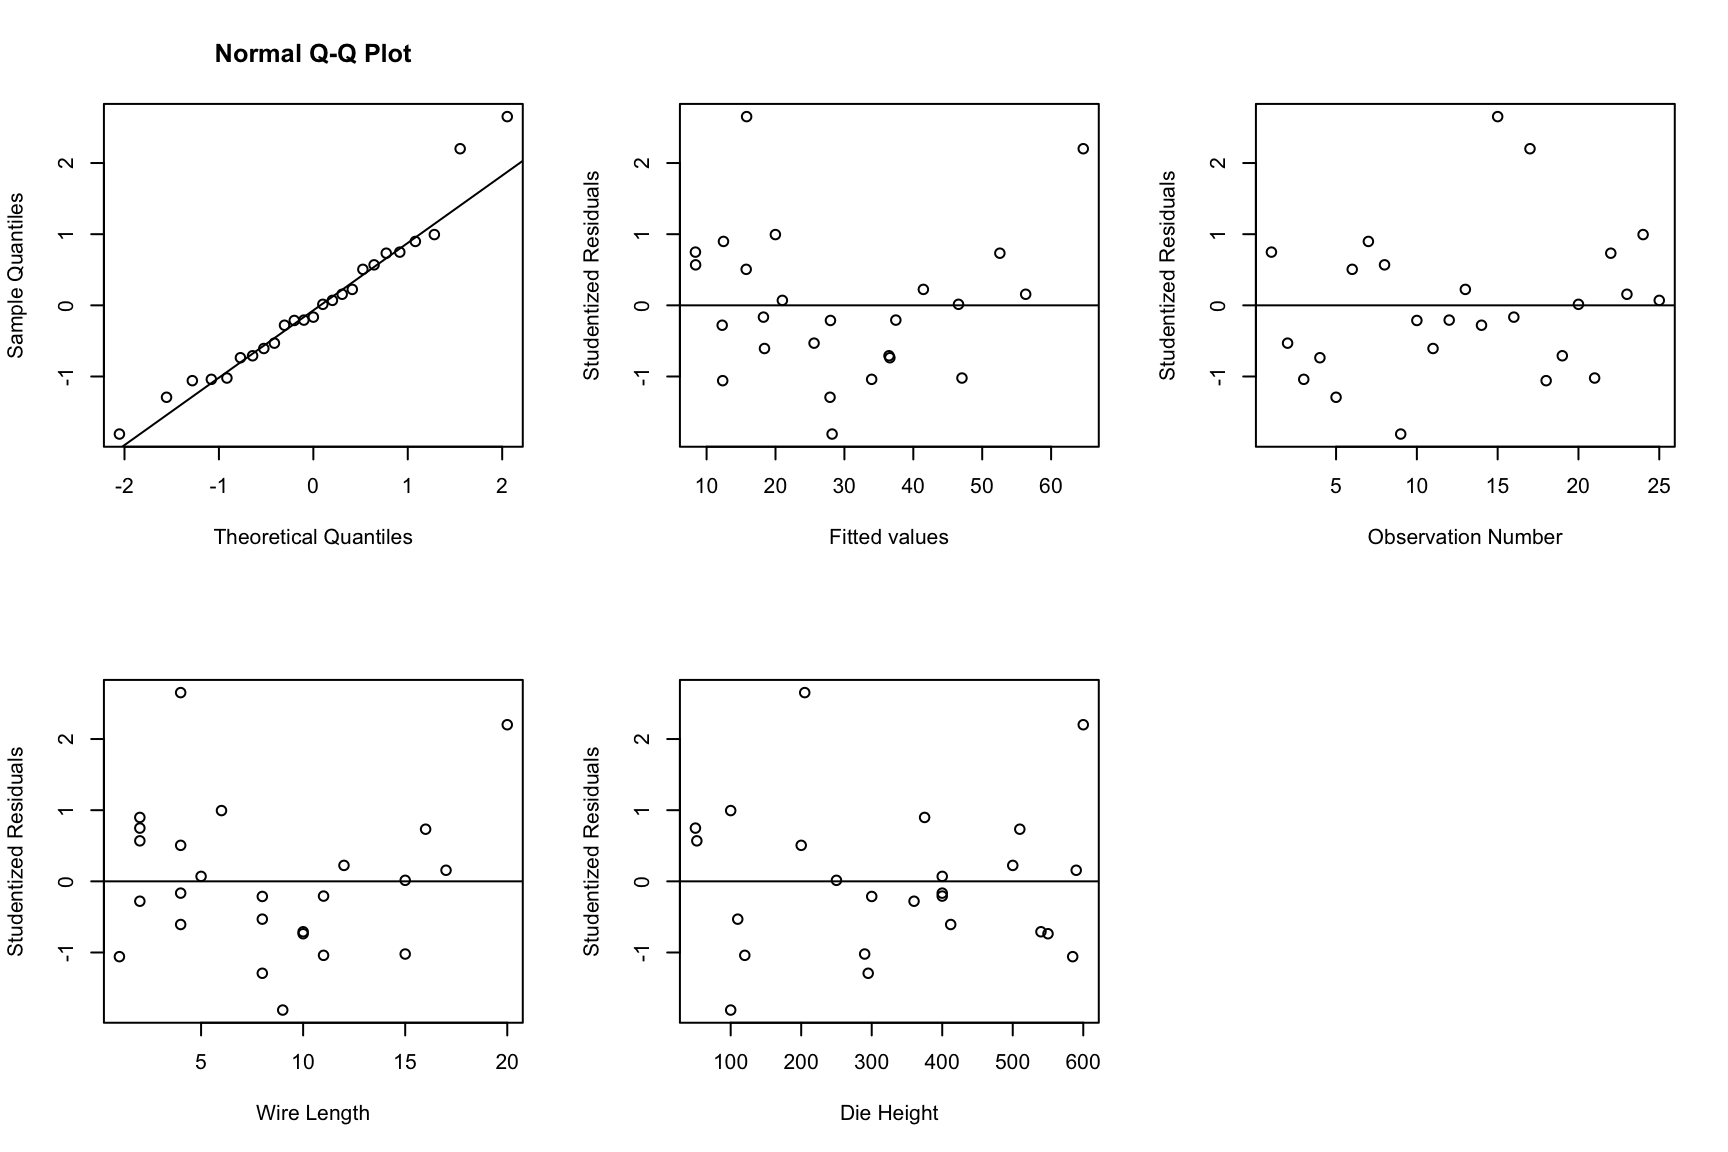
\includegraphics[keepaspectratio]{unit3-mlr/mlr_files/figure-pdf/unnamed-chunk-18-1.pdf}}

\section{Influential Observations}\label{influential-observations}

\begin{Shaded}
\begin{Highlighting}[]
\NormalTok{influence\_df }\OtherTok{\textless{}{-}} \FunctionTok{data.frame}\NormalTok{(}\AttributeTok{dffits =} \FunctionTok{dffits}\NormalTok{(fit),}
                           \AttributeTok{cook.D =} \FunctionTok{cooks.distance}\NormalTok{(fit),}
                           \FunctionTok{dfbetas}\NormalTok{(fit))}
\NormalTok{influence\_df}
\end{Highlighting}
\end{Shaded}

\begin{verbatim}
         dffits       cook.D  X.Intercept.       length       height
1   0.319854702 3.481748e-02  0.3179493921 -0.100534181 -0.200085326
2  -0.185251548 1.183028e-02 -0.1403477437 -0.051464370  0.148315370
3  -0.423741713 5.962023e-02 -0.2219151046 -0.237135616  0.339340552
4  -0.245376811 2.050736e-02  0.0787635526  0.022343842 -0.184260891
5  -0.274191565 2.426179e-02 -0.1572410603 -0.009662357  0.055328303
6   0.141461363 6.906752e-03  0.1301249135 -0.058073567 -0.049408295
7   0.327082639 3.598953e-02  0.1479853099 -0.261848970  0.142220906
8   0.240902557 1.996750e-02  0.2394962591 -0.076575387 -0.149787102
9  -0.733818383 1.600749e-01 -0.5011686139 -0.283749099  0.605559181
10 -0.043165927 6.493384e-04 -0.0241138520 -0.001038287  0.007460760
11 -0.190885522 1.251125e-02 -0.0602003847  0.132053762 -0.102733745
12 -0.047774650 7.954763e-04  0.0017554145 -0.016926531 -0.008495572
13  0.065496465 1.494604e-03 -0.0224255162  0.017340091  0.033756253
14 -0.097602753 3.314830e-03 -0.0483552961  0.077880727 -0.038066705
15  0.886553487 1.866936e-01  0.8097463528 -0.374290156 -0.292048214
16 -0.050292599 8.821617e-04 -0.0177647675  0.034746758 -0.025275682
17  1.441003392 5.654455e-01 -0.8513738015  1.008880052  0.413618783
18 -0.683268805 1.547244e-01 -0.0218935465  0.521608456 -0.532432956
19 -0.228476293 1.781295e-02  0.0700729860  0.018004228 -0.167581999
20  0.005805362 1.176892e-05  0.0005613509  0.004752581 -0.003094588
21 -0.394724862 5.182743e-02 -0.0084618169 -0.324109965  0.170622396
22  0.287343813 2.812893e-02 -0.1326208213  0.183002776  0.076391058
23  0.071903545 1.803448e-03 -0.0412553376  0.040164093  0.030365108
24  0.347915085 4.036930e-02  0.3084561584  0.016541769 -0.262089402
25  0.019115733 1.275757e-04  0.0062730782 -0.011614674  0.009459029
\end{verbatim}

\subsection{\texorpdfstring{Plotting with the \texttt{olsrr}
Package}{Plotting with the olsrr Package}}\label{plotting-with-the-olsrr-package}

\begin{Shaded}
\begin{Highlighting}[]
\CommentTok{\# install.packages("olsrr") \# Run once if needed}
\FunctionTok{library}\NormalTok{(olsrr)}

\FunctionTok{ols\_plot\_cooksd\_chart}\NormalTok{(fit)}
\end{Highlighting}
\end{Shaded}

\pandocbounded{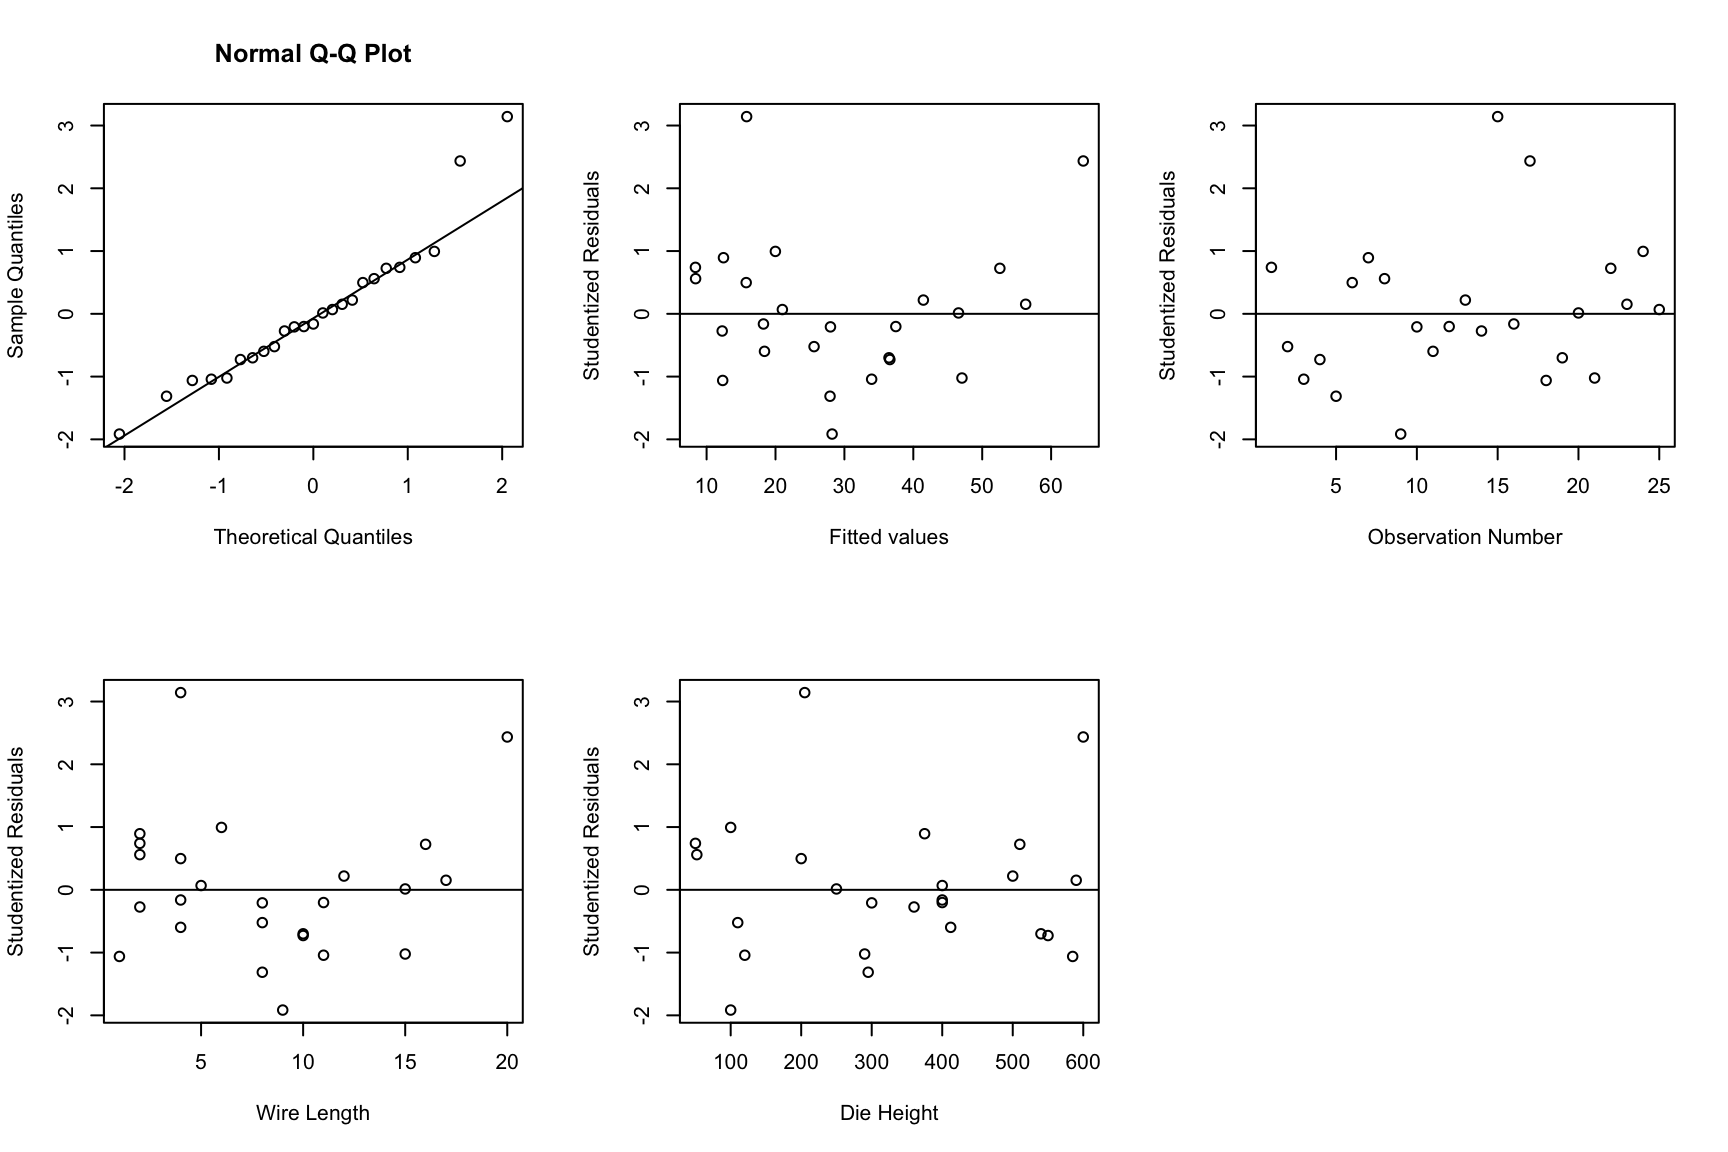
\includegraphics[keepaspectratio]{unit3-mlr/mlr_files/figure-pdf/unnamed-chunk-20-1.pdf}}

\begin{Shaded}
\begin{Highlighting}[]
\FunctionTok{ols\_plot\_dffits}\NormalTok{(fit)}
\end{Highlighting}
\end{Shaded}

\pandocbounded{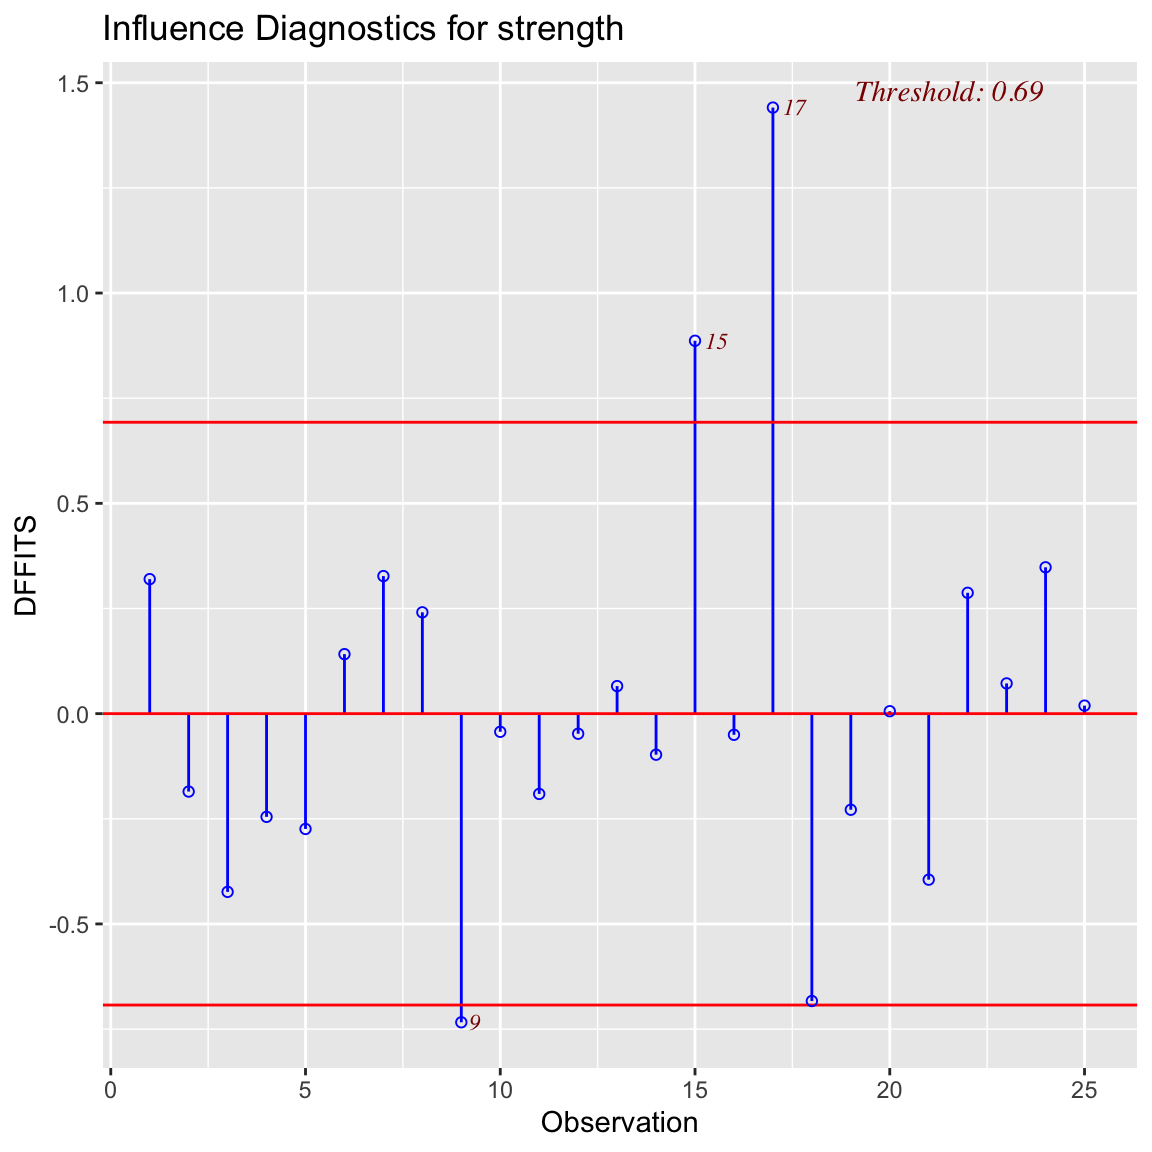
\includegraphics[keepaspectratio]{unit3-mlr/mlr_files/figure-pdf/unnamed-chunk-20-2.pdf}}

\begin{Shaded}
\begin{Highlighting}[]
\FunctionTok{ols\_plot\_dfbetas}\NormalTok{(fit)}
\end{Highlighting}
\end{Shaded}

\pandocbounded{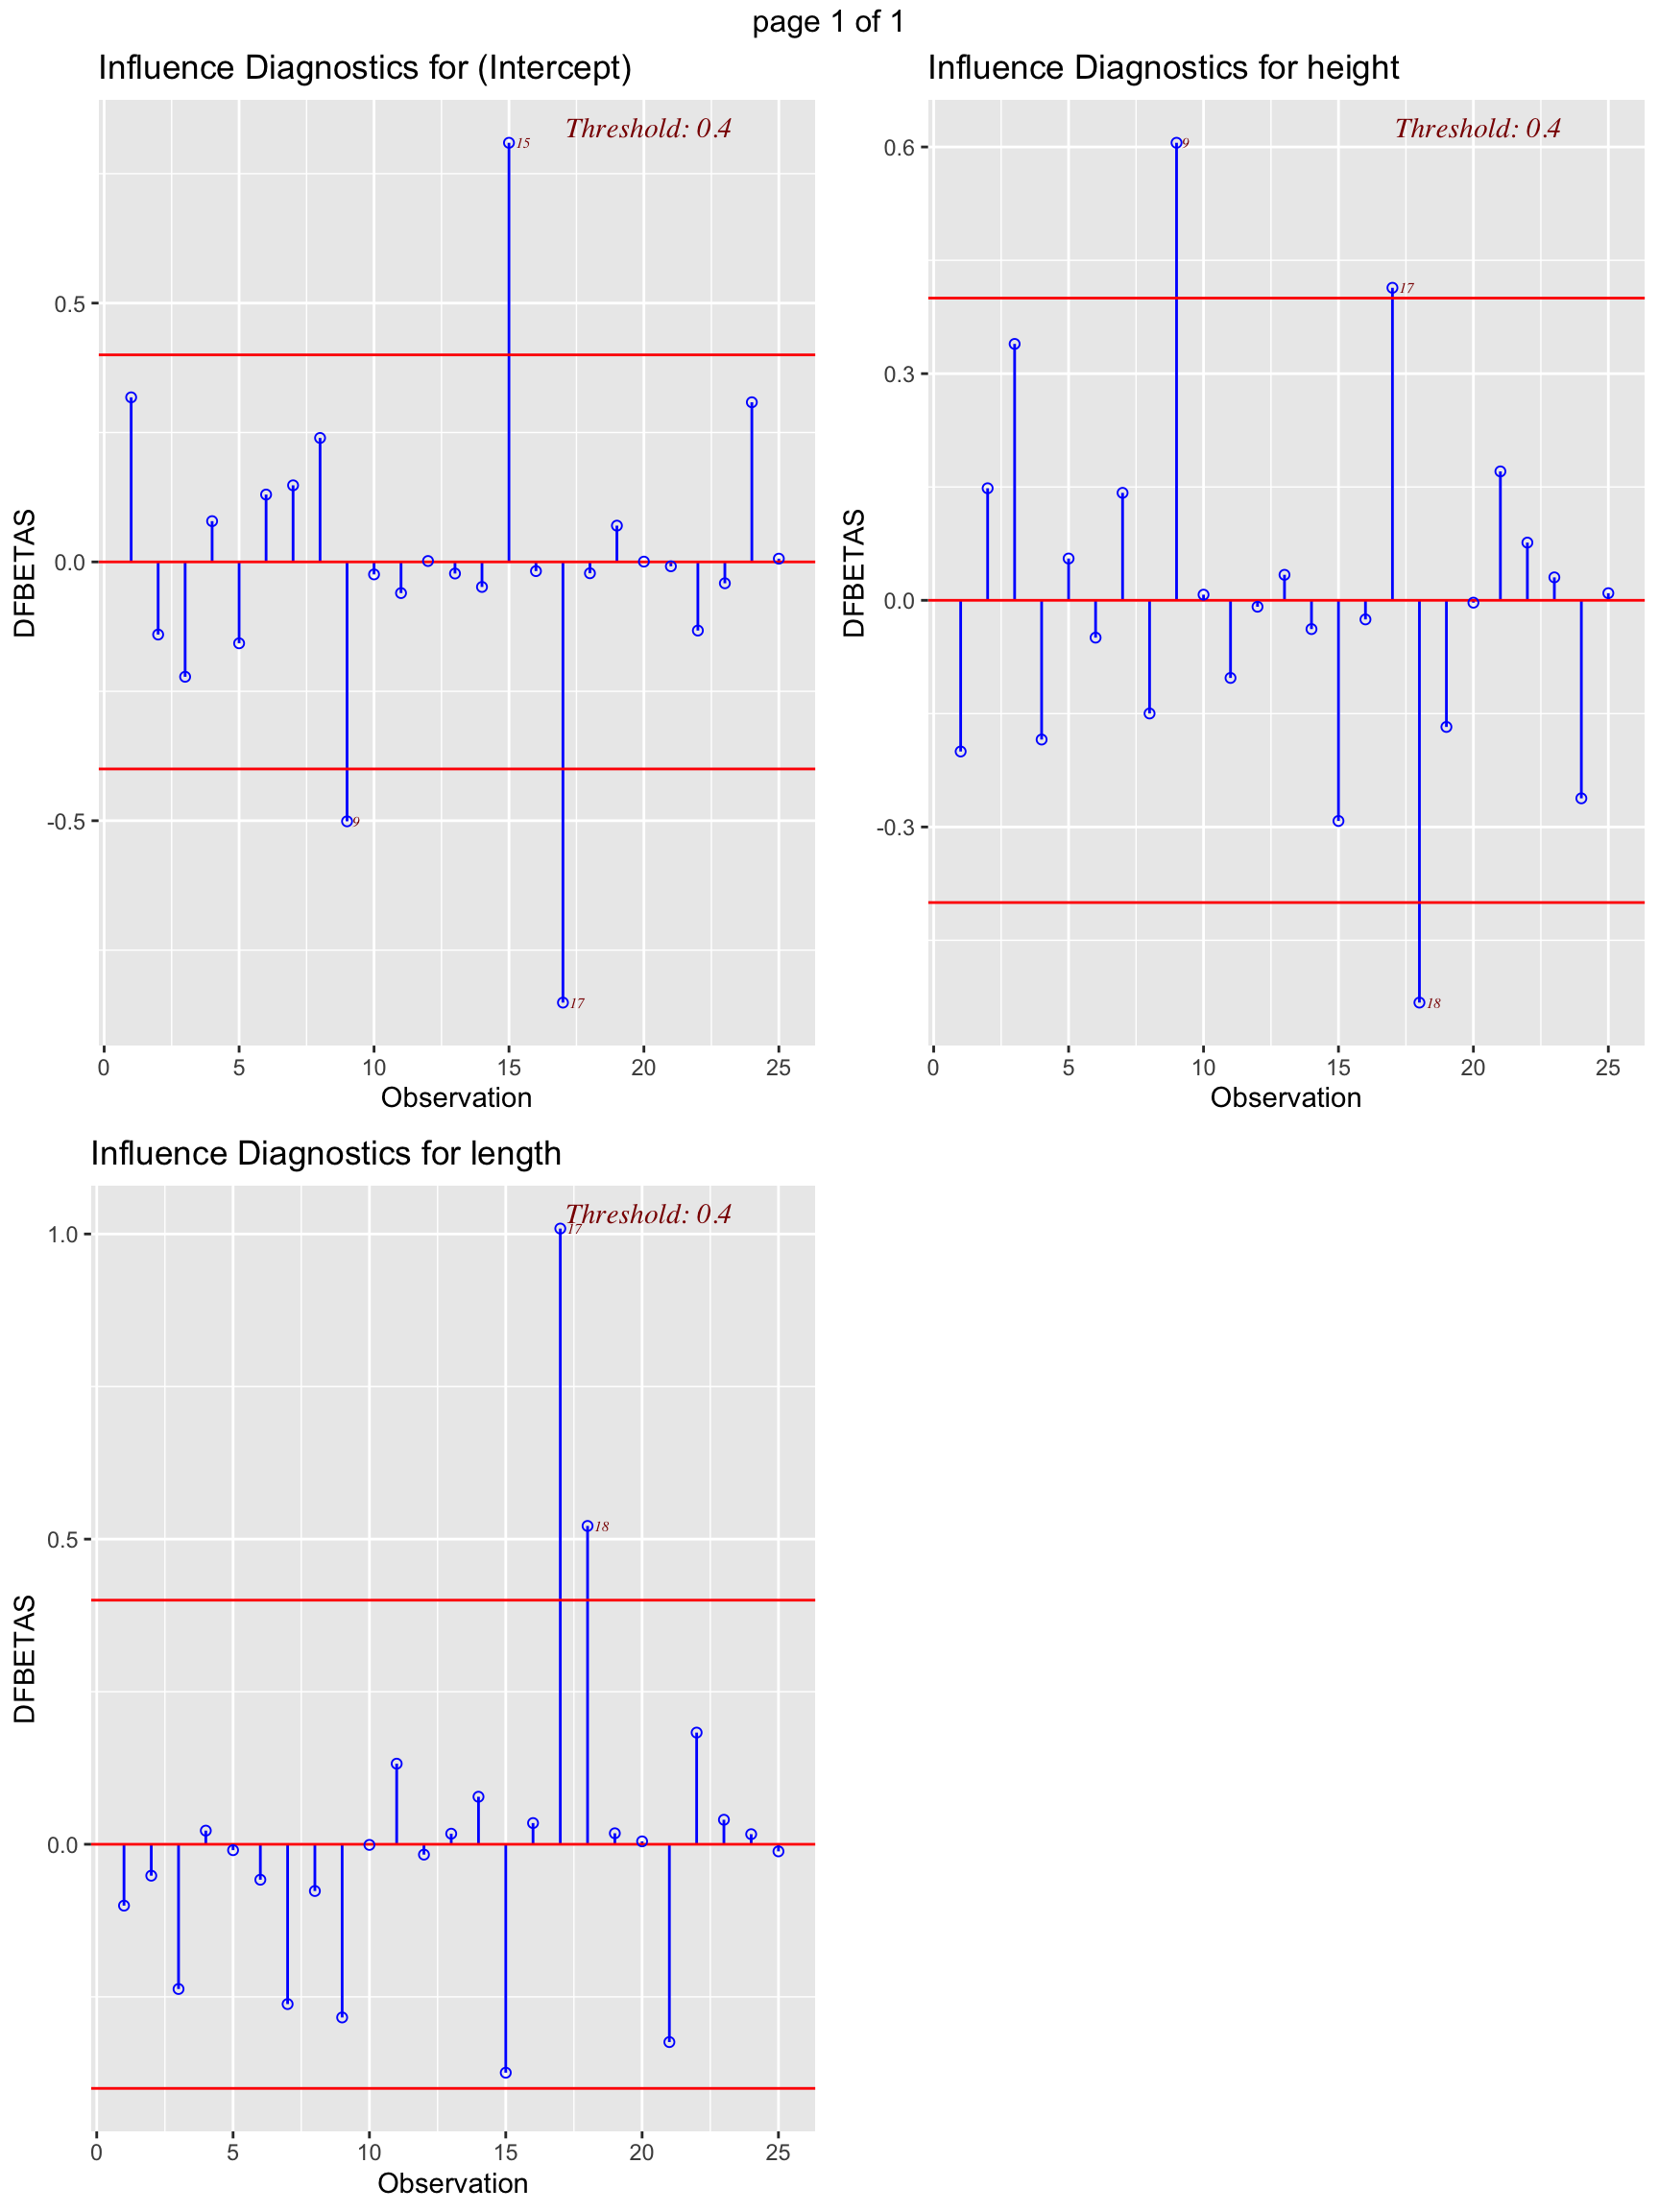
\includegraphics[keepaspectratio]{unit3-mlr/mlr_files/figure-pdf/unnamed-chunk-20-3.pdf}}

\section{Polynomial Regression}\label{polynomial-regression}

\begin{Shaded}
\begin{Highlighting}[]
\NormalTok{y }\OtherTok{\textless{}{-}} \FunctionTok{c}\NormalTok{(}\FloatTok{1.81}\NormalTok{, }\FloatTok{1.70}\NormalTok{, }\FloatTok{1.65}\NormalTok{, }\FloatTok{1.55}\NormalTok{, }\FloatTok{1.48}\NormalTok{, }\FloatTok{1.40}\NormalTok{, }\FloatTok{1.30}\NormalTok{, }\FloatTok{1.26}\NormalTok{, }\FloatTok{1.24}\NormalTok{, }\FloatTok{1.21}\NormalTok{, }\FloatTok{1.20}\NormalTok{, }\FloatTok{1.18}\NormalTok{)}
\NormalTok{x }\OtherTok{\textless{}{-}} \FunctionTok{c}\NormalTok{(}\DecValTok{20}\NormalTok{, }\DecValTok{25}\NormalTok{, }\DecValTok{30}\NormalTok{, }\DecValTok{35}\NormalTok{, }\DecValTok{40}\NormalTok{, }\DecValTok{50}\NormalTok{, }\DecValTok{60}\NormalTok{, }\DecValTok{65}\NormalTok{, }\DecValTok{70}\NormalTok{, }\DecValTok{75}\NormalTok{, }\DecValTok{80}\NormalTok{, }\DecValTok{90}\NormalTok{)}
\NormalTok{fit\_poly }\OtherTok{\textless{}{-}} \FunctionTok{lm}\NormalTok{(y }\SpecialCharTok{\textasciitilde{}}\NormalTok{ x }\SpecialCharTok{+} \FunctionTok{I}\NormalTok{(x}\SpecialCharTok{\^{}}\DecValTok{2}\NormalTok{))}
\FunctionTok{summary}\NormalTok{(fit\_poly)}
\end{Highlighting}
\end{Shaded}

\begin{verbatim}

Call:
lm(formula = y ~ x + I(x^2))

Residuals:
       Min         1Q     Median         3Q        Max 
-0.0174763 -0.0065087  0.0001297  0.0071482  0.0151887 

Coefficients:
              Estimate Std. Error t value Pr(>|t|)    
(Intercept)  2.198e+00  2.255e-02   97.48 6.38e-15 ***
x           -2.252e-02  9.424e-04  -23.90 1.88e-09 ***
I(x^2)       1.251e-04  8.658e-06   14.45 1.56e-07 ***
---
Signif. codes:  0 '***' 0.001 '**' 0.01 '*' 0.05 '.' 0.1 ' ' 1

Residual standard error: 0.01219 on 9 degrees of freedom
Multiple R-squared:  0.9975,    Adjusted R-squared:  0.9969 
F-statistic:  1767 on 2 and 9 DF,  p-value: 2.096e-12
\end{verbatim}

\begin{Shaded}
\begin{Highlighting}[]
\FunctionTok{plot}\NormalTok{(x, y, }\AttributeTok{xlab =} \StringTok{"Lot size, x"}\NormalTok{, }\AttributeTok{ylab =} \StringTok{"Average cost per unit, y"}\NormalTok{)}
\FunctionTok{lines}\NormalTok{(x, }\FunctionTok{predict}\NormalTok{(fit\_poly, }\AttributeTok{newdata =} \FunctionTok{data.frame}\NormalTok{(}\AttributeTok{x =}\NormalTok{ x)), }\AttributeTok{type =} \StringTok{"l"}\NormalTok{)}
\end{Highlighting}
\end{Shaded}

\pandocbounded{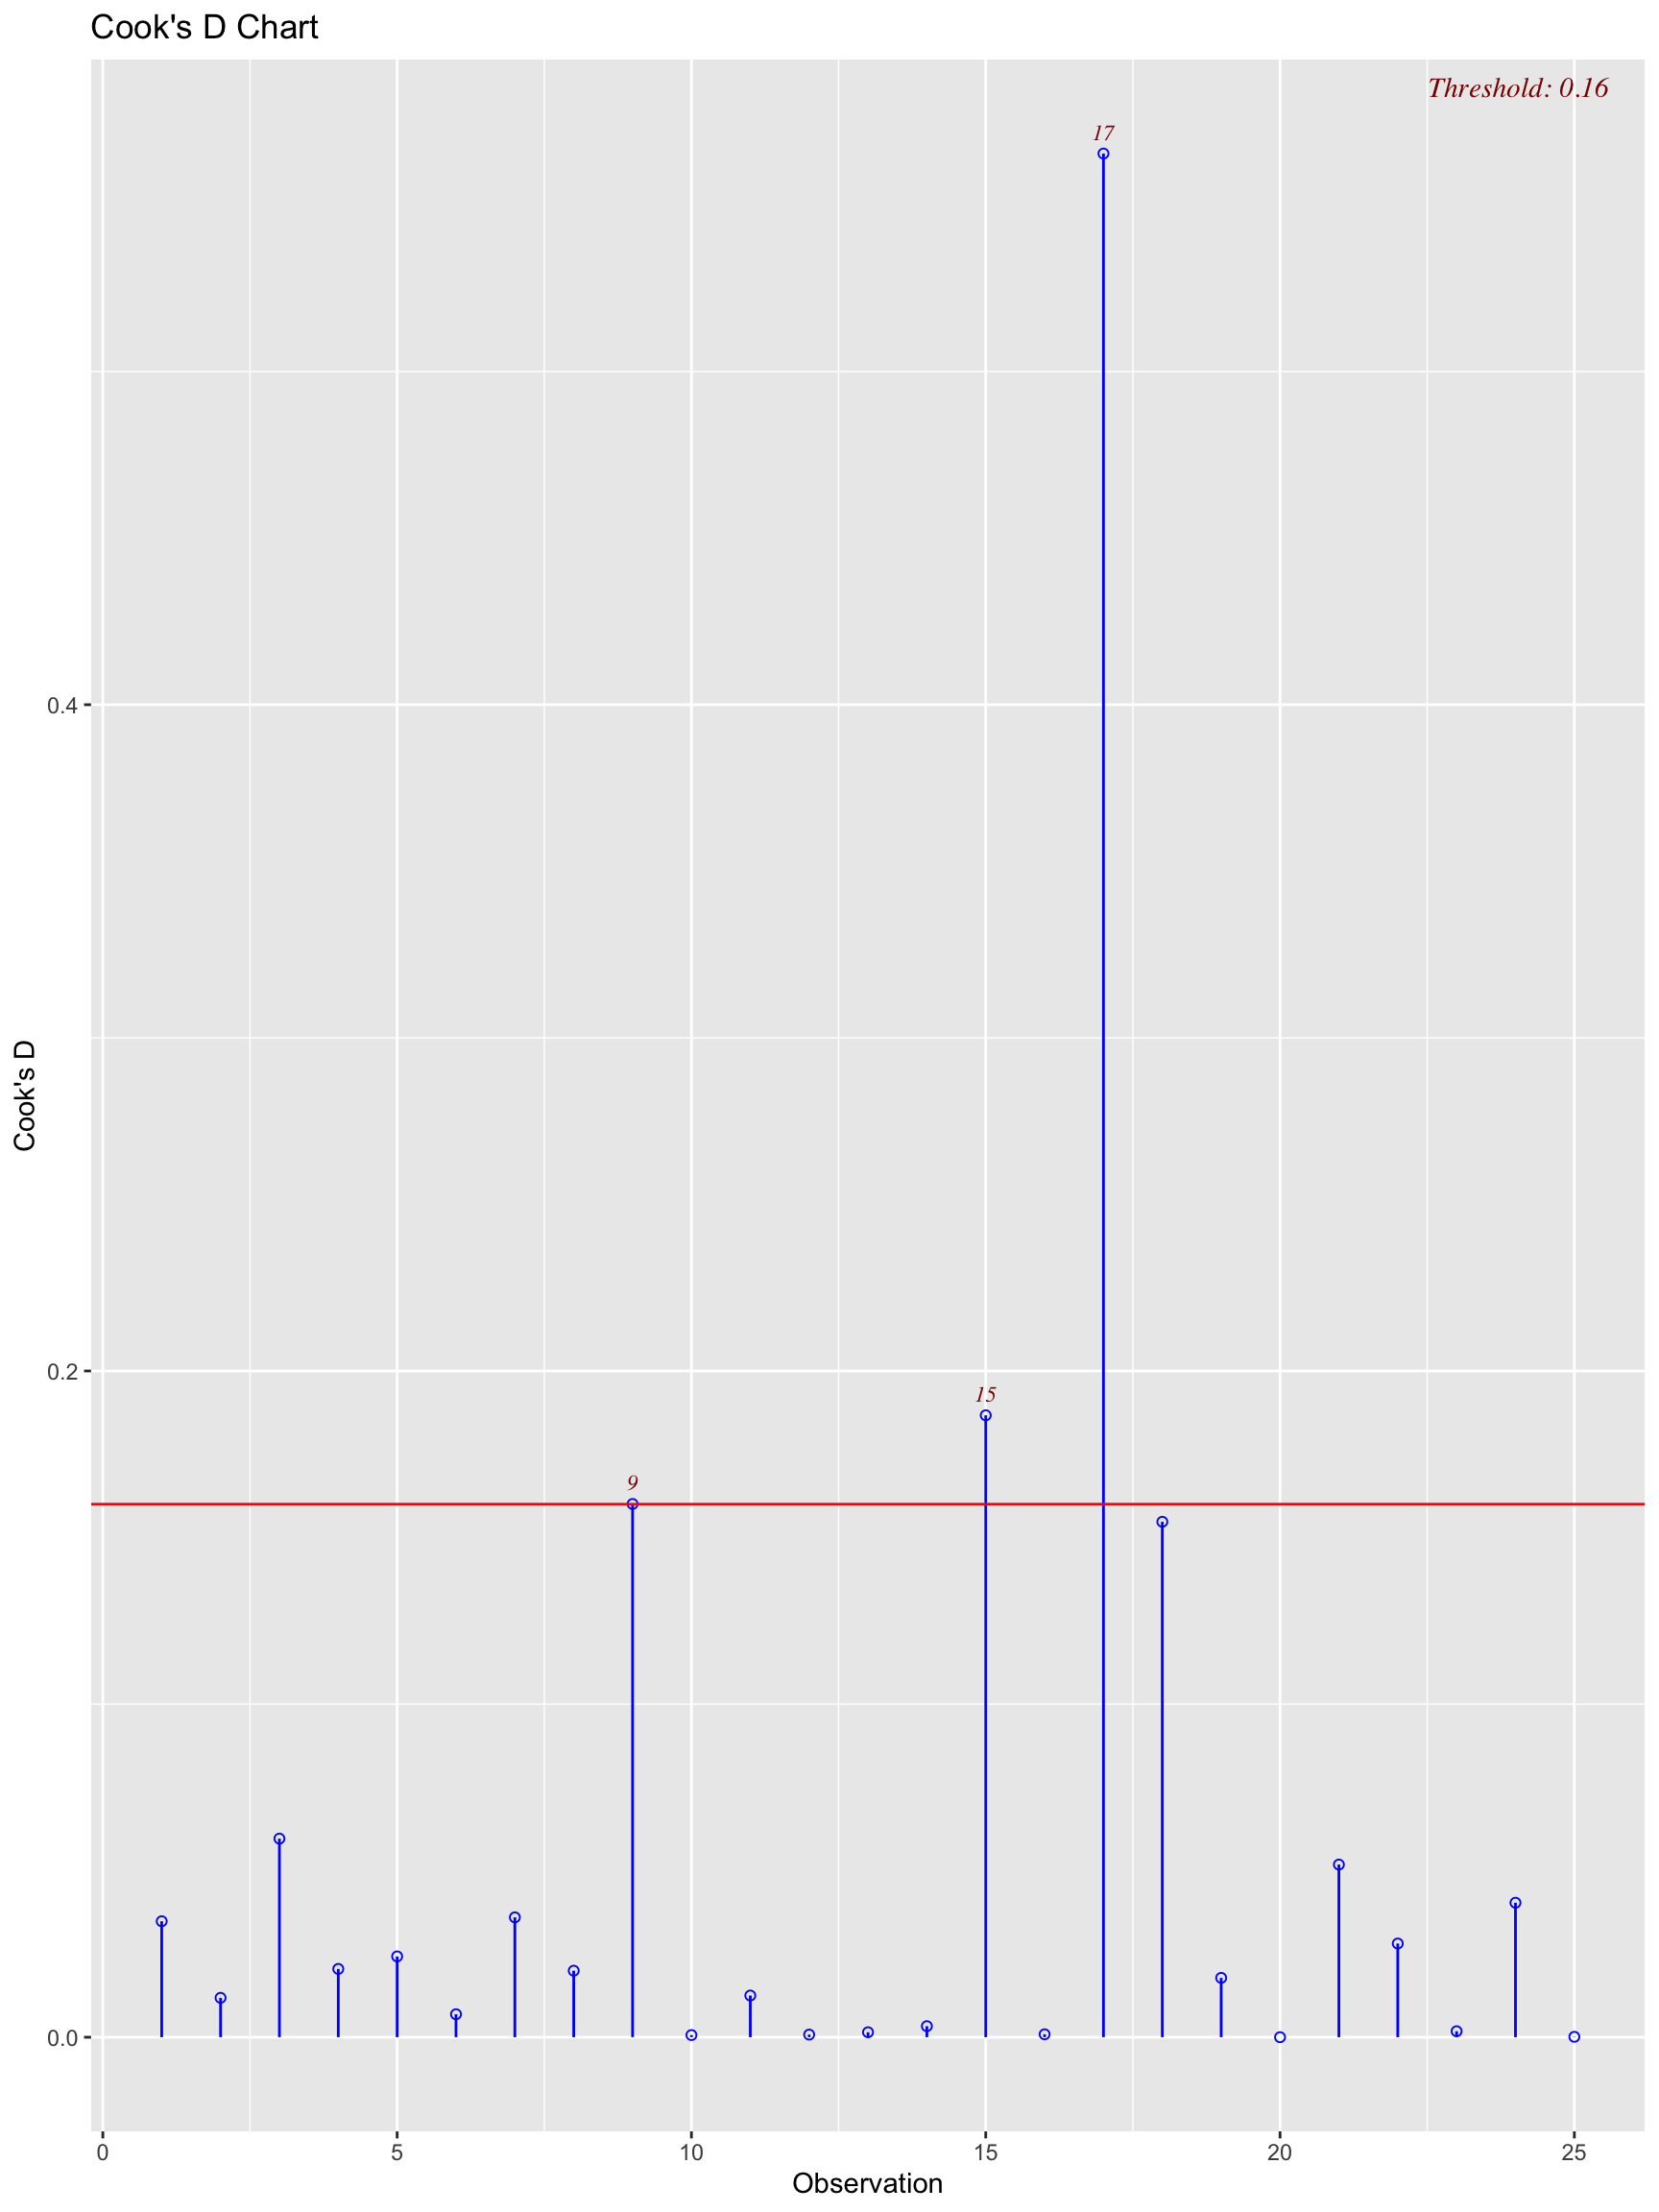
\includegraphics[keepaspectratio]{unit3-mlr/mlr_files/figure-pdf/unnamed-chunk-22-1.pdf}}

\begin{Shaded}
\begin{Highlighting}[]
\NormalTok{fit1 }\OtherTok{\textless{}{-}} \FunctionTok{lm}\NormalTok{(y }\SpecialCharTok{\textasciitilde{}}\NormalTok{ x)}
\FunctionTok{anova}\NormalTok{(fit1, fit\_poly)}
\end{Highlighting}
\end{Shaded}

\begin{verbatim}
Analysis of Variance Table

Model 1: y ~ x
Model 2: y ~ x + I(x^2)
  Res.Df      RSS Df Sum of Sq      F    Pr(>F)    
1     10 0.032340                                  
2      9 0.001337  1  0.031002 208.67 1.564e-07 ***
---
Signif. codes:  0 '***' 0.001 '**' 0.01 '*' 0.05 '.' 0.1 ' ' 1
\end{verbatim}

\section{Handling Categorical Variables with Dummy
Variables}\label{handling-categorical-variables-with-dummy-variables}

Investigate the common observation that males tend to have higher blood
pressure than females of similar age.

\begin{Shaded}
\begin{Highlighting}[]
\CommentTok{\# Note: Update this path to your local file location}
\NormalTok{sbpdata }\OtherTok{\textless{}{-}} \FunctionTok{read.csv}\NormalTok{(}\StringTok{"sbpdata.csv"}\NormalTok{)}
\NormalTok{sbpdata}
\end{Highlighting}
\end{Shaded}

\begin{verbatim}
   sex sbp age
1    0 144  39
2    0 138  45
3    0 145  47
4    0 162  65
5    0 142  46
6    0 170  67
7    0 124  42
8    0 158  67
9    0 154  56
10   0 162  64
11   0 150  56
12   0 140  59
13   0 110  34
14   0 128  42
15   0 130  48
16   0 135  45
17   0 114  17
18   0 116  20
19   0 124  19
20   0 136  36
21   0 142  50
22   0 120  39
23   0 120  21
24   0 160  44
25   0 158  53
26   0 144  63
27   0 130  29
28   0 125  25
29   0 175  69
30   1 158  41
31   1 185  60
32   1 152  41
33   1 159  47
34   1 176  66
35   1 156  47
36   1 184  68
37   1 138  43
38   1 172  68
39   1 168  57
40   1 176  65
41   1 164  57
42   1 154  61
43   1 124  36
44   1 142  44
45   1 144  50
46   1 149  47
47   1 128  19
48   1 130  22
49   1 138  21
50   1 150  38
51   1 156  52
52   1 134  41
53   1 134  18
54   1 174  51
55   1 174  55
56   1 158  65
57   1 144  33
58   1 139  23
59   1 180  70
60   1 165  56
61   1 172  62
62   1 160  51
63   1 157  48
64   1 170  59
65   1 153  40
66   1 148  35
67   1 140  33
68   1 132  26
69   1 169  61
\end{verbatim}

\subsection{Four Models Involving
``sex''}\label{four-models-involving-sex}

\subsubsection{Coincidence Model (Age
Only)}\label{coincidence-model-age-only}

\begin{Shaded}
\begin{Highlighting}[]
\CommentTok{\# Ensure sex is a factor (labels will appear in the legend)}
\NormalTok{sbpdata}\SpecialCharTok{$}\NormalTok{sex }\OtherTok{\textless{}{-}} \FunctionTok{as.factor}\NormalTok{(sbpdata}\SpecialCharTok{$}\NormalTok{sex)}

\CommentTok{\# Fit (you already have this)}
\NormalTok{fit.age }\OtherTok{\textless{}{-}} \FunctionTok{lm}\NormalTok{(sbp }\SpecialCharTok{\textasciitilde{}}\NormalTok{ age, }\AttributeTok{data =}\NormalTok{ sbpdata)}

\CommentTok{\# Generate predictions over the observed age range}
\NormalTok{new\_age }\OtherTok{\textless{}{-}} \FunctionTok{seq}\NormalTok{(}\FunctionTok{min}\NormalTok{(sbpdata}\SpecialCharTok{$}\NormalTok{age, }\AttributeTok{na.rm =} \ConstantTok{TRUE}\NormalTok{),}
               \FunctionTok{max}\NormalTok{(sbpdata}\SpecialCharTok{$}\NormalTok{age, }\AttributeTok{na.rm =} \ConstantTok{TRUE}\NormalTok{),}
               \AttributeTok{length.out =} \DecValTok{200}\NormalTok{)}
\NormalTok{pred }\OtherTok{\textless{}{-}} \FunctionTok{predict}\NormalTok{(fit.age, }\AttributeTok{newdata =} \FunctionTok{data.frame}\NormalTok{(}\AttributeTok{age =}\NormalTok{ new\_age))}

\CommentTok{\# Simple palette for the sex levels (works for 1–3 levels; expand if needed)}
\NormalTok{lev  }\OtherTok{\textless{}{-}} \FunctionTok{levels}\NormalTok{(sbpdata}\SpecialCharTok{$}\NormalTok{sex)}
\NormalTok{cols }\OtherTok{\textless{}{-}} \FunctionTok{setNames}\NormalTok{(}\FunctionTok{c}\NormalTok{(}\StringTok{"steelblue3"}\NormalTok{, }\StringTok{"tomato3"}\NormalTok{, }\StringTok{"darkorchid3"}\NormalTok{)[}\FunctionTok{seq\_along}\NormalTok{(lev)], lev)}

\CommentTok{\# Scatter plot with colored points by sex}
\FunctionTok{plot}\NormalTok{(sbp }\SpecialCharTok{\textasciitilde{}}\NormalTok{ age, }\AttributeTok{data =}\NormalTok{ sbpdata,}
     \AttributeTok{col =}\NormalTok{ cols[sbpdata}\SpecialCharTok{$}\NormalTok{sex], }\AttributeTok{pch =} \DecValTok{16}\NormalTok{,}
     \AttributeTok{xlab =} \StringTok{"Age"}\NormalTok{, }\AttributeTok{ylab =} \StringTok{"Systolic BP"}\NormalTok{)}

\CommentTok{\# Add predicted line}
\FunctionTok{lines}\NormalTok{(new\_age, pred, }\AttributeTok{lwd =} \DecValTok{2}\NormalTok{)}

\CommentTok{\# Legend}
\FunctionTok{legend}\NormalTok{(}\StringTok{"topleft"}\NormalTok{, }\AttributeTok{legend =}\NormalTok{ lev, }\AttributeTok{col =}\NormalTok{ cols[lev], }\AttributeTok{pch =} \DecValTok{16}\NormalTok{, }\AttributeTok{bty =} \StringTok{"n"}\NormalTok{, }\AttributeTok{title =} \StringTok{"Sex"}\NormalTok{)}
\end{Highlighting}
\end{Shaded}

\pandocbounded{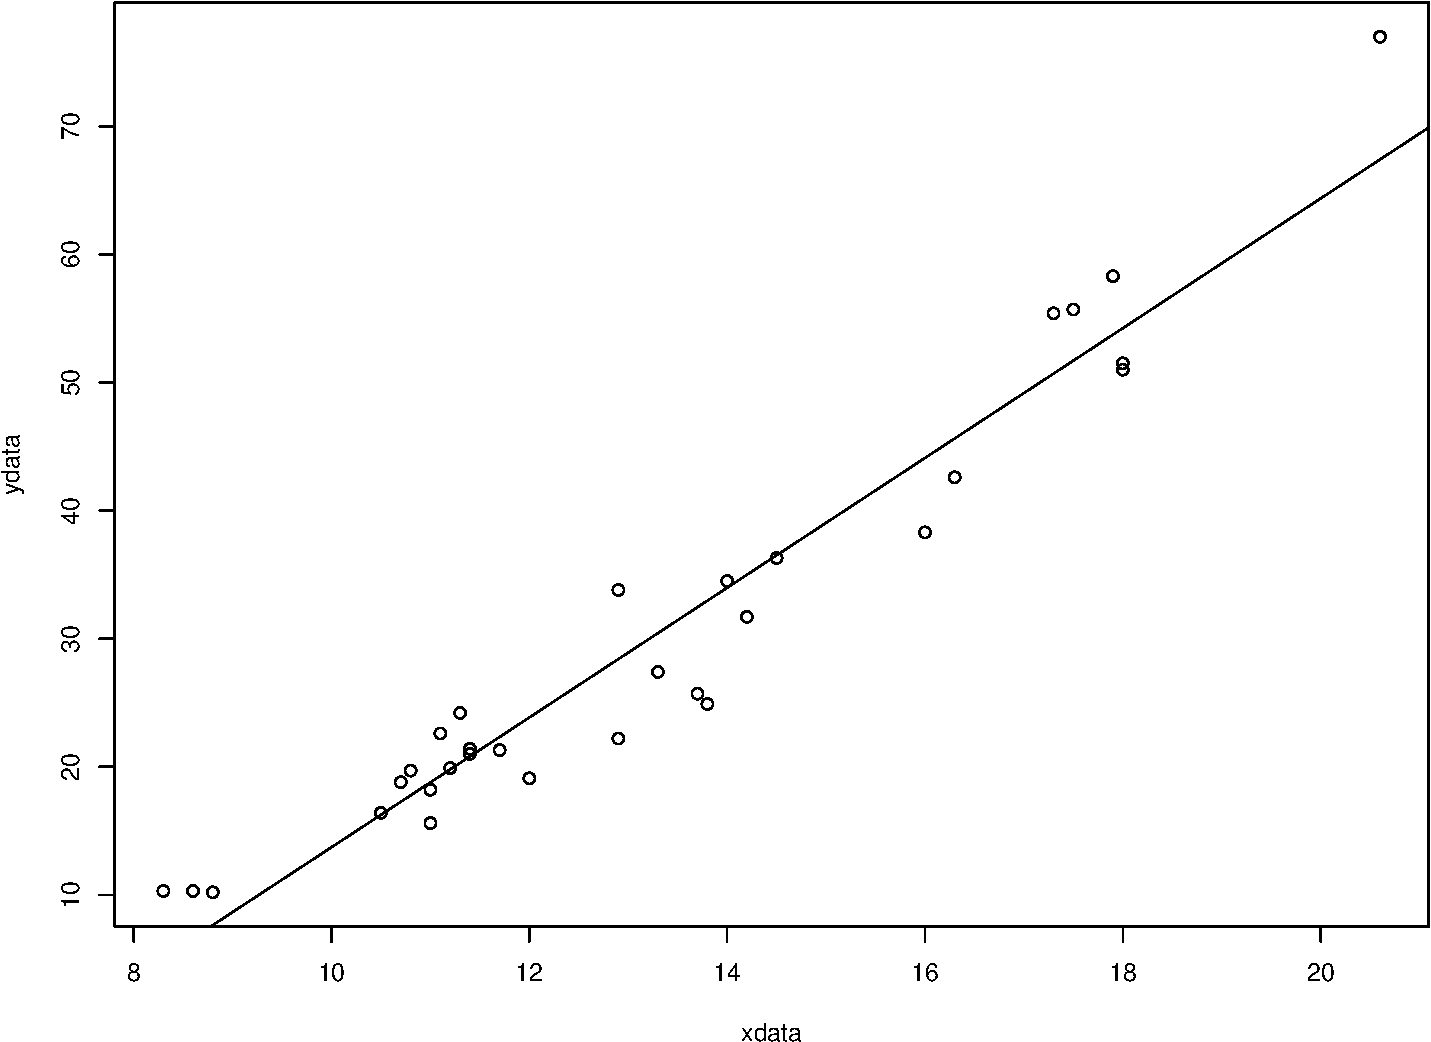
\includegraphics[keepaspectratio]{unit3-mlr/mlr_files/figure-pdf/unnamed-chunk-25-1.pdf}}

\begin{Shaded}
\begin{Highlighting}[]
\FunctionTok{data.frame}\NormalTok{(}\FunctionTok{model.matrix}\NormalTok{(fit.age)) }
\end{Highlighting}
\end{Shaded}

\begin{verbatim}
   X.Intercept. age
1             1  39
2             1  45
3             1  47
4             1  65
5             1  46
6             1  67
7             1  42
8             1  67
9             1  56
10            1  64
11            1  56
12            1  59
13            1  34
14            1  42
15            1  48
16            1  45
17            1  17
18            1  20
19            1  19
20            1  36
21            1  50
22            1  39
23            1  21
24            1  44
25            1  53
26            1  63
27            1  29
28            1  25
29            1  69
30            1  41
31            1  60
32            1  41
33            1  47
34            1  66
35            1  47
36            1  68
37            1  43
38            1  68
39            1  57
40            1  65
41            1  57
42            1  61
43            1  36
44            1  44
45            1  50
46            1  47
47            1  19
48            1  22
49            1  21
50            1  38
51            1  52
52            1  41
53            1  18
54            1  51
55            1  55
56            1  65
57            1  33
58            1  23
59            1  70
60            1  56
61            1  62
62            1  51
63            1  48
64            1  59
65            1  40
66            1  35
67            1  33
68            1  26
69            1  61
\end{verbatim}

\begin{Shaded}
\begin{Highlighting}[]
\FunctionTok{print}\NormalTok{(}\FunctionTok{anova}\NormalTok{(fit.age))}
\end{Highlighting}
\end{Shaded}

\begin{verbatim}
Analysis of Variance Table

Response: sbp
          Df  Sum Sq Mean Sq F value    Pr(>F)    
age        1 14951.3 14951.3  121.27 < 2.2e-16 ***
Residuals 67  8260.5   123.3                      
---
Signif. codes:  0 '***' 0.001 '**' 0.01 '*' 0.05 '.' 0.1 ' ' 1
\end{verbatim}

\subsubsection{Additive Effect Model (Age +
Sex)}\label{additive-effect-model-age-sex}

\begin{Shaded}
\begin{Highlighting}[]
\CommentTok{\# Parallelism: H0: beta3=0 (Sex has additive effect)}
\NormalTok{fit.agePLUSsex }\OtherTok{\textless{}{-}} \FunctionTok{lm}\NormalTok{(sbp }\SpecialCharTok{\textasciitilde{}}\NormalTok{ age }\SpecialCharTok{+}\NormalTok{ sex, }\AttributeTok{data =}\NormalTok{ sbpdata)}

\CommentTok{\# Ensure sex is a factor for labeling/colors}
\NormalTok{sbpdata}\SpecialCharTok{$}\NormalTok{sex }\OtherTok{\textless{}{-}} \FunctionTok{factor}\NormalTok{(sbpdata}\SpecialCharTok{$}\NormalTok{sex)}

\CommentTok{\# Fit (additive: parallelism)}
\NormalTok{fit.agePLUSsex }\OtherTok{\textless{}{-}} \FunctionTok{lm}\NormalTok{(sbp }\SpecialCharTok{\textasciitilde{}}\NormalTok{ age }\SpecialCharTok{+}\NormalTok{ sex, }\AttributeTok{data =}\NormalTok{ sbpdata)}

\CommentTok{\# X{-}range and palette}
\NormalTok{ages }\OtherTok{\textless{}{-}} \FunctionTok{seq}\NormalTok{(}\FunctionTok{min}\NormalTok{(sbpdata}\SpecialCharTok{$}\NormalTok{age, }\AttributeTok{na.rm =} \ConstantTok{TRUE}\NormalTok{),}
            \FunctionTok{max}\NormalTok{(sbpdata}\SpecialCharTok{$}\NormalTok{age, }\AttributeTok{na.rm =} \ConstantTok{TRUE}\NormalTok{),}
            \AttributeTok{length.out =} \DecValTok{200}\NormalTok{)}
\NormalTok{lev  }\OtherTok{\textless{}{-}} \FunctionTok{levels}\NormalTok{(sbpdata}\SpecialCharTok{$}\NormalTok{sex)}
\NormalTok{cols }\OtherTok{\textless{}{-}} \FunctionTok{setNames}\NormalTok{(}\FunctionTok{c}\NormalTok{(}\StringTok{"steelblue3"}\NormalTok{, }\StringTok{"tomato3"}\NormalTok{, }\StringTok{"darkorchid3"}\NormalTok{)[}\FunctionTok{seq\_along}\NormalTok{(lev)], lev)}

\CommentTok{\# Scatter with colored points by sex}
\FunctionTok{plot}\NormalTok{(sbp }\SpecialCharTok{\textasciitilde{}}\NormalTok{ age, }\AttributeTok{data =}\NormalTok{ sbpdata,}
     \AttributeTok{col =}\NormalTok{ cols[sbpdata}\SpecialCharTok{$}\NormalTok{sex], }\AttributeTok{pch =} \DecValTok{16}\NormalTok{,}
     \AttributeTok{xlab =} \StringTok{"Age"}\NormalTok{, }\AttributeTok{ylab =} \StringTok{"Systolic BP"}\NormalTok{)}

\CommentTok{\# Parallel fitted lines: one per sex (same slope, different intercepts)}
\ControlFlowTok{for}\NormalTok{ (sx }\ControlFlowTok{in}\NormalTok{ lev) \{}
\NormalTok{  nd }\OtherTok{\textless{}{-}} \FunctionTok{data.frame}\NormalTok{(}\AttributeTok{age =}\NormalTok{ ages, }\AttributeTok{sex =} \FunctionTok{factor}\NormalTok{(sx, }\AttributeTok{levels =}\NormalTok{ lev))}
\NormalTok{  yhat }\OtherTok{\textless{}{-}} \FunctionTok{predict}\NormalTok{(fit.agePLUSsex, }\AttributeTok{newdata =}\NormalTok{ nd)}
  \FunctionTok{lines}\NormalTok{(ages, yhat, }\AttributeTok{col =}\NormalTok{ cols[sx], }\AttributeTok{lwd =} \DecValTok{2}\NormalTok{)}
\NormalTok{\}}

\CommentTok{\# Legend}
\FunctionTok{legend}\NormalTok{(}\StringTok{"topleft"}\NormalTok{, }\AttributeTok{legend =}\NormalTok{ lev, }\AttributeTok{col =}\NormalTok{ cols[lev], }\AttributeTok{pch =} \DecValTok{16}\NormalTok{, }\AttributeTok{lwd =} \DecValTok{2}\NormalTok{, }\AttributeTok{bty =} \StringTok{"n"}\NormalTok{, }\AttributeTok{title =} \StringTok{"Sex"}\NormalTok{)}
\end{Highlighting}
\end{Shaded}

\pandocbounded{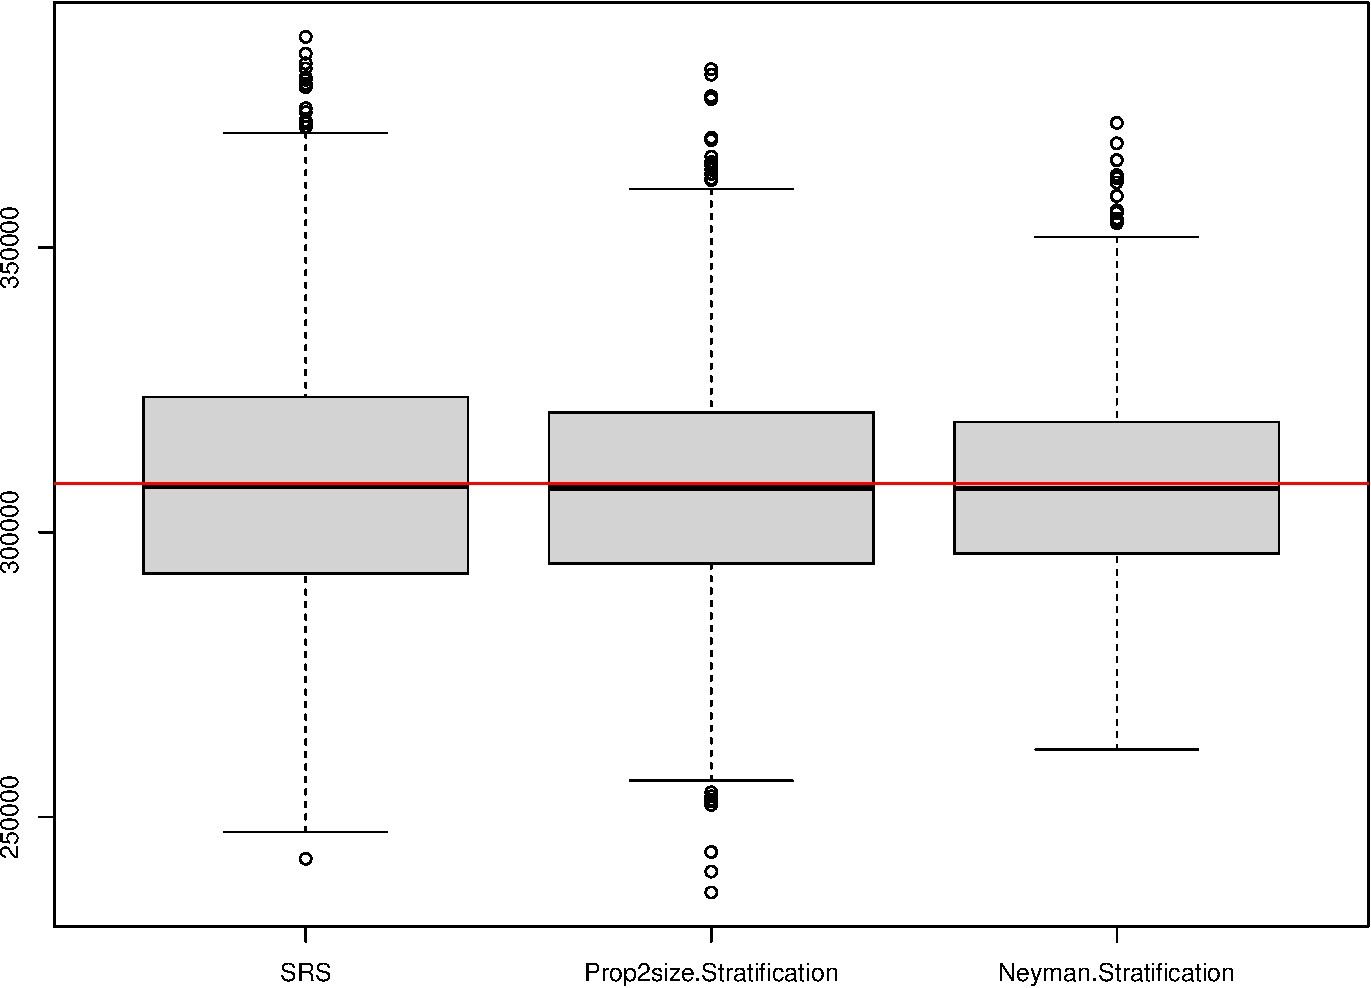
\includegraphics[keepaspectratio]{unit3-mlr/mlr_files/figure-pdf/unnamed-chunk-27-1.pdf}}

\begin{Shaded}
\begin{Highlighting}[]
\FunctionTok{data.frame}\NormalTok{(}\FunctionTok{model.matrix}\NormalTok{(fit.agePLUSsex))}
\end{Highlighting}
\end{Shaded}

\begin{verbatim}
   X.Intercept. age sex1
1             1  39    0
2             1  45    0
3             1  47    0
4             1  65    0
5             1  46    0
6             1  67    0
7             1  42    0
8             1  67    0
9             1  56    0
10            1  64    0
11            1  56    0
12            1  59    0
13            1  34    0
14            1  42    0
15            1  48    0
16            1  45    0
17            1  17    0
18            1  20    0
19            1  19    0
20            1  36    0
21            1  50    0
22            1  39    0
23            1  21    0
24            1  44    0
25            1  53    0
26            1  63    0
27            1  29    0
28            1  25    0
29            1  69    0
30            1  41    1
31            1  60    1
32            1  41    1
33            1  47    1
34            1  66    1
35            1  47    1
36            1  68    1
37            1  43    1
38            1  68    1
39            1  57    1
40            1  65    1
41            1  57    1
42            1  61    1
43            1  36    1
44            1  44    1
45            1  50    1
46            1  47    1
47            1  19    1
48            1  22    1
49            1  21    1
50            1  38    1
51            1  52    1
52            1  41    1
53            1  18    1
54            1  51    1
55            1  55    1
56            1  65    1
57            1  33    1
58            1  23    1
59            1  70    1
60            1  56    1
61            1  62    1
62            1  51    1
63            1  48    1
64            1  59    1
65            1  40    1
66            1  35    1
67            1  33    1
68            1  26    1
69            1  61    1
\end{verbatim}

\begin{Shaded}
\begin{Highlighting}[]
\FunctionTok{print}\NormalTok{(}\FunctionTok{anova}\NormalTok{(fit.age, fit.agePLUSsex))}
\end{Highlighting}
\end{Shaded}

\begin{verbatim}
Analysis of Variance Table

Model 1: sbp ~ age
Model 2: sbp ~ age + sex
  Res.Df    RSS Df Sum of Sq      F    Pr(>F)    
1     67 8260.5                                  
2     66 5202.0  1    3058.5 38.805 3.701e-08 ***
---
Signif. codes:  0 '***' 0.001 '**' 0.01 '*' 0.05 '.' 0.1 ' ' 1
\end{verbatim}

\subsubsection{Varying Intercept and Varying Slope Model (Age + Sex +
Age:Sex)}\label{varying-intercept-and-varying-slope-model-age-sex-agesex}

\begin{Shaded}
\begin{Highlighting}[]
\CommentTok{\# Make sure sex is a factor (for colors/legend)}
\NormalTok{sbpdata}\SpecialCharTok{$}\NormalTok{sex }\OtherTok{\textless{}{-}} \FunctionTok{factor}\NormalTok{(sbpdata}\SpecialCharTok{$}\NormalTok{sex)}

\CommentTok{\# Fit (interaction: different slopes by sex)}
\NormalTok{fit.age.TIMES.sex }\OtherTok{\textless{}{-}} \FunctionTok{lm}\NormalTok{(sbp }\SpecialCharTok{\textasciitilde{}}\NormalTok{ age }\SpecialCharTok{+}\NormalTok{ sex }\SpecialCharTok{+}\NormalTok{ age}\SpecialCharTok{:}\NormalTok{sex, }\AttributeTok{data =}\NormalTok{ sbpdata)}

\CommentTok{\# Age grid and palette}
\NormalTok{ages }\OtherTok{\textless{}{-}} \FunctionTok{seq}\NormalTok{(}\FunctionTok{min}\NormalTok{(sbpdata}\SpecialCharTok{$}\NormalTok{age, }\AttributeTok{na.rm =} \ConstantTok{TRUE}\NormalTok{),}
            \FunctionTok{max}\NormalTok{(sbpdata}\SpecialCharTok{$}\NormalTok{age, }\AttributeTok{na.rm =} \ConstantTok{TRUE}\NormalTok{),}
            \AttributeTok{length.out =} \DecValTok{200}\NormalTok{)}
\NormalTok{lev  }\OtherTok{\textless{}{-}} \FunctionTok{levels}\NormalTok{(sbpdata}\SpecialCharTok{$}\NormalTok{sex)}
\NormalTok{cols }\OtherTok{\textless{}{-}} \FunctionTok{setNames}\NormalTok{(}\FunctionTok{c}\NormalTok{(}\StringTok{"steelblue3"}\NormalTok{, }\StringTok{"tomato3"}\NormalTok{, }\StringTok{"darkorchid3"}\NormalTok{)[}\FunctionTok{seq\_along}\NormalTok{(lev)], lev)}

\CommentTok{\# Scatter: color points by sex}
\FunctionTok{plot}\NormalTok{(sbp }\SpecialCharTok{\textasciitilde{}}\NormalTok{ age, }\AttributeTok{data =}\NormalTok{ sbpdata,}
     \AttributeTok{col =}\NormalTok{ cols[sbpdata}\SpecialCharTok{$}\NormalTok{sex], }\AttributeTok{pch =} \DecValTok{16}\NormalTok{,}
     \AttributeTok{xlab =} \StringTok{"Age"}\NormalTok{, }\AttributeTok{ylab =} \StringTok{"Systolic BP"}\NormalTok{)}

\CommentTok{\# Fitted lines: one per sex (different slopes allowed)}
\ControlFlowTok{for}\NormalTok{ (sx }\ControlFlowTok{in}\NormalTok{ lev) \{}
\NormalTok{  nd }\OtherTok{\textless{}{-}} \FunctionTok{data.frame}\NormalTok{(}\AttributeTok{age =}\NormalTok{ ages, }\AttributeTok{sex =} \FunctionTok{factor}\NormalTok{(sx, }\AttributeTok{levels =}\NormalTok{ lev))}
\NormalTok{  yhat }\OtherTok{\textless{}{-}} \FunctionTok{predict}\NormalTok{(fit.age.TIMES.sex, }\AttributeTok{newdata =}\NormalTok{ nd)}
  \FunctionTok{lines}\NormalTok{(ages, yhat, }\AttributeTok{col =}\NormalTok{ cols[sx], }\AttributeTok{lwd =} \DecValTok{2}\NormalTok{)}
\NormalTok{\}}

\CommentTok{\# Legend}
\FunctionTok{legend}\NormalTok{(}\StringTok{"topleft"}\NormalTok{, }\AttributeTok{legend =}\NormalTok{ lev, }\AttributeTok{col =}\NormalTok{ cols[lev], }\AttributeTok{pch =} \DecValTok{16}\NormalTok{, }\AttributeTok{lwd =} \DecValTok{2}\NormalTok{, }\AttributeTok{bty =} \StringTok{"n"}\NormalTok{, }\AttributeTok{title =} \StringTok{"Sex"}\NormalTok{)}
\end{Highlighting}
\end{Shaded}

\pandocbounded{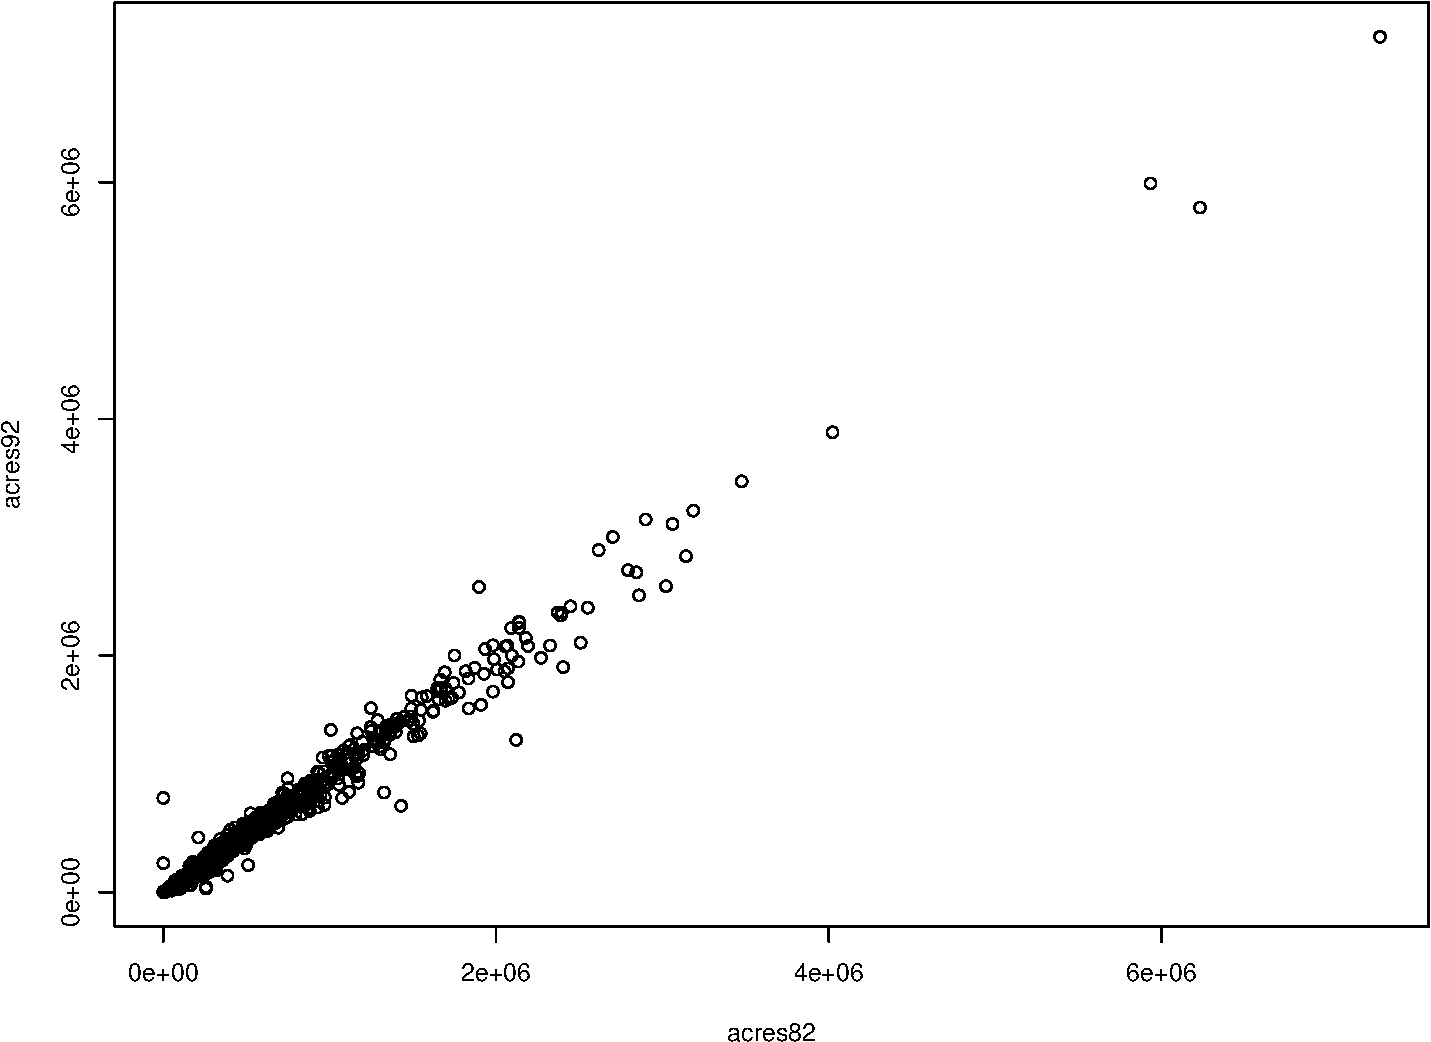
\includegraphics[keepaspectratio]{unit3-mlr/mlr_files/figure-pdf/unnamed-chunk-29-1.pdf}}

\textbf{Model Matrix and ANOVA}

\begin{Shaded}
\begin{Highlighting}[]
\FunctionTok{data.frame}\NormalTok{(}\FunctionTok{model.matrix}\NormalTok{(fit.age.TIMES.sex))}
\end{Highlighting}
\end{Shaded}

\begin{verbatim}
   X.Intercept. age sex1 age.sex1
1             1  39    0        0
2             1  45    0        0
3             1  47    0        0
4             1  65    0        0
5             1  46    0        0
6             1  67    0        0
7             1  42    0        0
8             1  67    0        0
9             1  56    0        0
10            1  64    0        0
11            1  56    0        0
12            1  59    0        0
13            1  34    0        0
14            1  42    0        0
15            1  48    0        0
16            1  45    0        0
17            1  17    0        0
18            1  20    0        0
19            1  19    0        0
20            1  36    0        0
21            1  50    0        0
22            1  39    0        0
23            1  21    0        0
24            1  44    0        0
25            1  53    0        0
26            1  63    0        0
27            1  29    0        0
28            1  25    0        0
29            1  69    0        0
30            1  41    1       41
31            1  60    1       60
32            1  41    1       41
33            1  47    1       47
34            1  66    1       66
35            1  47    1       47
36            1  68    1       68
37            1  43    1       43
38            1  68    1       68
39            1  57    1       57
40            1  65    1       65
41            1  57    1       57
42            1  61    1       61
43            1  36    1       36
44            1  44    1       44
45            1  50    1       50
46            1  47    1       47
47            1  19    1       19
48            1  22    1       22
49            1  21    1       21
50            1  38    1       38
51            1  52    1       52
52            1  41    1       41
53            1  18    1       18
54            1  51    1       51
55            1  55    1       55
56            1  65    1       65
57            1  33    1       33
58            1  23    1       23
59            1  70    1       70
60            1  56    1       56
61            1  62    1       62
62            1  51    1       51
63            1  48    1       48
64            1  59    1       59
65            1  40    1       40
66            1  35    1       35
67            1  33    1       33
68            1  26    1       26
69            1  61    1       61
\end{verbatim}

\begin{Shaded}
\begin{Highlighting}[]
\FunctionTok{summary}\NormalTok{(fit.age.TIMES.sex)}
\end{Highlighting}
\end{Shaded}

\begin{verbatim}

Call:
lm(formula = sbp ~ age + sex + age:sex, data = sbpdata)

Residuals:
    Min      1Q  Median      3Q     Max 
-20.647  -3.410   1.254   4.314  21.153 

Coefficients:
            Estimate Std. Error t value Pr(>|t|)    
(Intercept) 97.07708    5.17046  18.775  < 2e-16 ***
age          0.94932    0.10864   8.738 1.43e-12 ***
sex1        12.96144    7.01172   1.849   0.0691 .  
age:sex1     0.01203    0.14519   0.083   0.9342    
---
Signif. codes:  0 '***' 0.001 '**' 0.01 '*' 0.05 '.' 0.1 ' ' 1

Residual standard error: 8.946 on 65 degrees of freedom
Multiple R-squared:  0.7759,    Adjusted R-squared:  0.7656 
F-statistic: 75.02 on 3 and 65 DF,  p-value: < 2.2e-16
\end{verbatim}

\begin{Shaded}
\begin{Highlighting}[]
\FunctionTok{print}\NormalTok{(}\FunctionTok{anova}\NormalTok{(fit.age,fit.agePLUSsex,fit.age.TIMES.sex))}
\end{Highlighting}
\end{Shaded}

\begin{verbatim}
Analysis of Variance Table

Model 1: sbp ~ age
Model 2: sbp ~ age + sex
Model 3: sbp ~ age + sex + age:sex
  Res.Df    RSS Df Sum of Sq       F    Pr(>F)    
1     67 8260.5                                   
2     66 5202.0  1   3058.52 38.2210 4.692e-08 ***
3     65 5201.4  1      0.55  0.0069    0.9342    
---
Signif. codes:  0 '***' 0.001 '**' 0.01 '*' 0.05 '.' 0.1 ' ' 1
\end{verbatim}

\subsubsection{Varying Slope, Equal Intercept Model (Age +
Age:Sex)}\label{varying-slope-equal-intercept-model-age-agesex}

\begin{Shaded}
\begin{Highlighting}[]
\CommentTok{\# Make sure sex is a factor (for colors/legend)}
\NormalTok{sbpdata}\SpecialCharTok{$}\NormalTok{sex }\OtherTok{\textless{}{-}} \FunctionTok{factor}\NormalTok{(sbpdata}\SpecialCharTok{$}\NormalTok{sex)}

\CommentTok{\# Fit (interaction: different slopes by sex)}
\NormalTok{fit.equal.intercept }\OtherTok{\textless{}{-}} \FunctionTok{lm}\NormalTok{(sbp }\SpecialCharTok{\textasciitilde{}}\NormalTok{ age }\SpecialCharTok{+}\NormalTok{ age}\SpecialCharTok{:}\NormalTok{sex, }\AttributeTok{data =}\NormalTok{ sbpdata)}


\CommentTok{\# Age grid and palette}
\NormalTok{ages }\OtherTok{\textless{}{-}} \FunctionTok{seq}\NormalTok{(}\FunctionTok{min}\NormalTok{(sbpdata}\SpecialCharTok{$}\NormalTok{age, }\AttributeTok{na.rm =} \ConstantTok{TRUE}\NormalTok{),}
            \FunctionTok{max}\NormalTok{(sbpdata}\SpecialCharTok{$}\NormalTok{age, }\AttributeTok{na.rm =} \ConstantTok{TRUE}\NormalTok{),}
            \AttributeTok{length.out =} \DecValTok{200}\NormalTok{)}
\NormalTok{lev  }\OtherTok{\textless{}{-}} \FunctionTok{levels}\NormalTok{(sbpdata}\SpecialCharTok{$}\NormalTok{sex)}
\NormalTok{cols }\OtherTok{\textless{}{-}} \FunctionTok{setNames}\NormalTok{(}\FunctionTok{c}\NormalTok{(}\StringTok{"steelblue3"}\NormalTok{, }\StringTok{"tomato3"}\NormalTok{, }\StringTok{"darkorchid3"}\NormalTok{)[}\FunctionTok{seq\_along}\NormalTok{(lev)], lev)}

\CommentTok{\# Scatter: color points by sex}
\FunctionTok{plot}\NormalTok{(sbp }\SpecialCharTok{\textasciitilde{}}\NormalTok{ age, }\AttributeTok{data =}\NormalTok{ sbpdata,}
     \AttributeTok{col =}\NormalTok{ cols[sbpdata}\SpecialCharTok{$}\NormalTok{sex], }\AttributeTok{pch =} \DecValTok{16}\NormalTok{,}
     \AttributeTok{xlab =} \StringTok{"Age"}\NormalTok{, }\AttributeTok{ylab =} \StringTok{"Systolic BP"}\NormalTok{)}

\CommentTok{\# Fitted lines: one per sex (different slopes allowed)}
\ControlFlowTok{for}\NormalTok{ (sx }\ControlFlowTok{in}\NormalTok{ lev) \{}
\NormalTok{  nd }\OtherTok{\textless{}{-}} \FunctionTok{data.frame}\NormalTok{(}\AttributeTok{age =}\NormalTok{ ages, }\AttributeTok{sex =} \FunctionTok{factor}\NormalTok{(sx, }\AttributeTok{levels =}\NormalTok{ lev))}
\NormalTok{  yhat }\OtherTok{\textless{}{-}} \FunctionTok{predict}\NormalTok{(fit.equal.intercept, }\AttributeTok{newdata =}\NormalTok{ nd)}
  \FunctionTok{lines}\NormalTok{(ages, yhat, }\AttributeTok{col =}\NormalTok{ cols[sx], }\AttributeTok{lwd =} \DecValTok{2}\NormalTok{)}
\NormalTok{\}}

\CommentTok{\# Legend}
\FunctionTok{legend}\NormalTok{(}\StringTok{"topleft"}\NormalTok{, }\AttributeTok{legend =}\NormalTok{ lev, }\AttributeTok{col =}\NormalTok{ cols[lev], }\AttributeTok{pch =} \DecValTok{16}\NormalTok{, }\AttributeTok{lwd =} \DecValTok{2}\NormalTok{, }\AttributeTok{bty =} \StringTok{"n"}\NormalTok{, }\AttributeTok{title =} \StringTok{"Sex"}\NormalTok{)}
\end{Highlighting}
\end{Shaded}

\pandocbounded{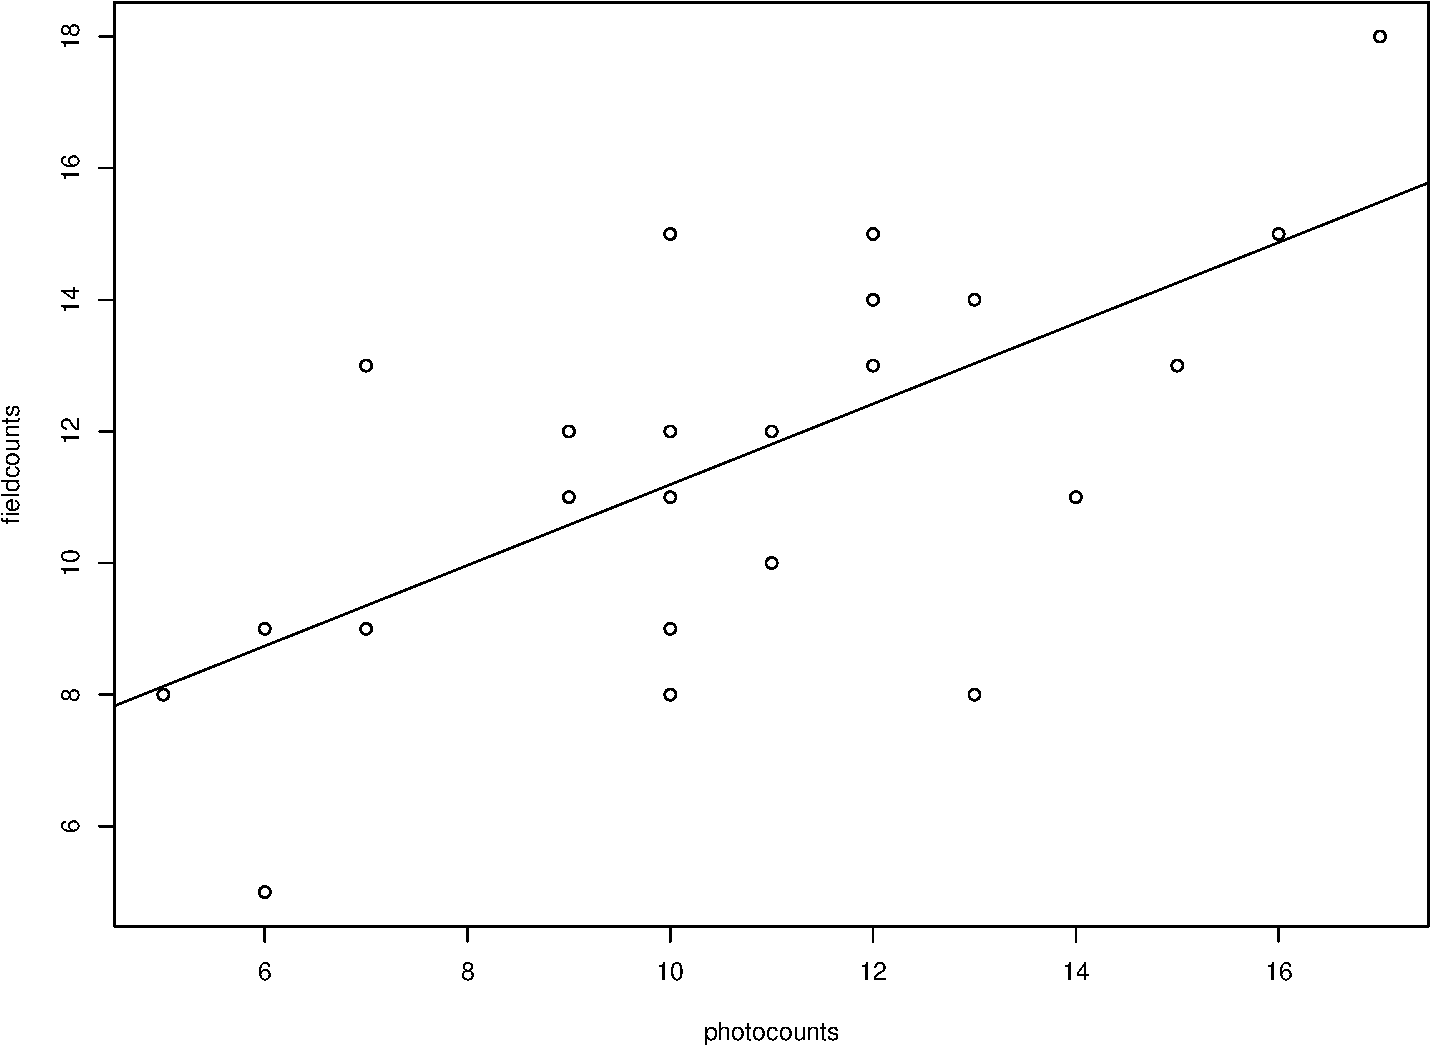
\includegraphics[keepaspectratio]{unit3-mlr/mlr_files/figure-pdf/unnamed-chunk-31-1.pdf}}

\subsection{Orders of Terms Matters in ANOVA and Warnings in
Interpreting t-test
Tables}\label{orders-of-terms-matters-in-anova-and-warnings-in-interpreting-t-test-tables}

\begin{Shaded}
\begin{Highlighting}[]
\NormalTok{fit.int }\OtherTok{\textless{}{-}} \FunctionTok{lm}\NormalTok{(sbp }\SpecialCharTok{\textasciitilde{}} \DecValTok{1}\NormalTok{, }\AttributeTok{data =}\NormalTok{ sbpdata)}
\NormalTok{fit.sex }\OtherTok{\textless{}{-}} \FunctionTok{lm}\NormalTok{(sbp }\SpecialCharTok{\textasciitilde{}}\NormalTok{ sex, }\AttributeTok{data =}\NormalTok{ sbpdata)}

\FunctionTok{print}\NormalTok{(}\FunctionTok{anova}\NormalTok{(fit.int,fit.age,fit.agePLUSsex, fit.age.TIMES.sex))}
\end{Highlighting}
\end{Shaded}

\begin{verbatim}
Analysis of Variance Table

Model 1: sbp ~ 1
Model 2: sbp ~ age
Model 3: sbp ~ age + sex
Model 4: sbp ~ age + sex + age:sex
  Res.Df     RSS Df Sum of Sq        F    Pr(>F)    
1     68 23211.8                                    
2     67  8260.5  1   14951.3 186.8390 < 2.2e-16 ***
3     66  5202.0  1    3058.5  38.2210 4.692e-08 ***
4     65  5201.4  1       0.5   0.0069    0.9342    
---
Signif. codes:  0 '***' 0.001 '**' 0.01 '*' 0.05 '.' 0.1 ' ' 1
\end{verbatim}

\begin{Shaded}
\begin{Highlighting}[]
\FunctionTok{print}\NormalTok{(}\FunctionTok{anova}\NormalTok{(fit.int,fit.age,fit.equal.intercept, fit.age.TIMES.sex))}
\end{Highlighting}
\end{Shaded}

\begin{verbatim}
Analysis of Variance Table

Model 1: sbp ~ 1
Model 2: sbp ~ age
Model 3: sbp ~ age + age:sex
Model 4: sbp ~ age + sex + age:sex
  Res.Df     RSS Df Sum of Sq        F    Pr(>F)    
1     68 23211.8                                    
2     67  8260.5  1   14951.3 186.8390 < 2.2e-16 ***
3     66  5474.9  1    2785.6  34.8107 1.437e-07 ***
4     65  5201.4  1     273.4   3.4171   0.06907 .  
---
Signif. codes:  0 '***' 0.001 '**' 0.01 '*' 0.05 '.' 0.1 ' ' 1
\end{verbatim}

\begin{Shaded}
\begin{Highlighting}[]
\FunctionTok{print}\NormalTok{(}\FunctionTok{anova}\NormalTok{(fit.int,fit.sex,fit.agePLUSsex, fit.age.TIMES.sex))}
\end{Highlighting}
\end{Shaded}

\begin{verbatim}
Analysis of Variance Table

Model 1: sbp ~ 1
Model 2: sbp ~ sex
Model 3: sbp ~ age + sex
Model 4: sbp ~ age + sex + age:sex
  Res.Df     RSS Df Sum of Sq        F    Pr(>F)    
1     68 23211.8                                    
2     67 19282.5  1    3929.2  49.1017 1.684e-09 ***
3     66  5202.0  1   14080.6 175.9583 < 2.2e-16 ***
4     65  5201.4  1       0.5   0.0069    0.9342    
---
Signif. codes:  0 '***' 0.001 '**' 0.01 '*' 0.05 '.' 0.1 ' ' 1
\end{verbatim}

\begin{Shaded}
\begin{Highlighting}[]
\FunctionTok{summary}\NormalTok{(fit.age)}
\end{Highlighting}
\end{Shaded}

\begin{verbatim}

Call:
lm(formula = sbp ~ age, data = sbpdata)

Residuals:
    Min      1Q  Median      3Q     Max 
-26.782  -7.632   1.968   8.201  22.651 

Coefficients:
             Estimate Std. Error t value Pr(>|t|)    
(Intercept) 103.34905    4.33190   23.86   <2e-16 ***
age           0.98333    0.08929   11.01   <2e-16 ***
---
Signif. codes:  0 '***' 0.001 '**' 0.01 '*' 0.05 '.' 0.1 ' ' 1

Residual standard error: 11.1 on 67 degrees of freedom
Multiple R-squared:  0.6441,    Adjusted R-squared:  0.6388 
F-statistic: 121.3 on 1 and 67 DF,  p-value: < 2.2e-16
\end{verbatim}

\begin{Shaded}
\begin{Highlighting}[]
\FunctionTok{summary}\NormalTok{(fit.equal.intercept)}
\end{Highlighting}
\end{Shaded}

\begin{verbatim}

Call:
lm(formula = sbp ~ age + age:sex, data = sbpdata)

Residuals:
     Min       1Q   Median       3Q      Max 
-21.6338  -4.3067   0.9922   4.9819  20.2753 

Coefficients:
             Estimate Std. Error t value Pr(>|t|)    
(Intercept) 104.12501    3.55578  29.283  < 2e-16 ***
age           0.80908    0.07918  10.219 3.14e-15 ***
age:sex1      0.26705    0.04608   5.795 2.09e-07 ***
---
Signif. codes:  0 '***' 0.001 '**' 0.01 '*' 0.05 '.' 0.1 ' ' 1

Residual standard error: 9.108 on 66 degrees of freedom
Multiple R-squared:  0.7641,    Adjusted R-squared:  0.757 
F-statistic: 106.9 on 2 and 66 DF,  p-value: < 2.2e-16
\end{verbatim}

\begin{Shaded}
\begin{Highlighting}[]
\FunctionTok{summary}\NormalTok{(fit.agePLUSsex)}
\end{Highlighting}
\end{Shaded}

\begin{verbatim}

Call:
lm(formula = sbp ~ age + sex, data = sbpdata)

Residuals:
    Min      1Q  Median      3Q     Max 
-20.705  -3.299   1.248   4.325  21.160 

Coefficients:
            Estimate Std. Error t value Pr(>|t|)    
(Intercept) 96.77353    3.62085  26.727  < 2e-16 ***
age          0.95606    0.07153  13.366  < 2e-16 ***
sex1        13.51345    2.16932   6.229  3.7e-08 ***
---
Signif. codes:  0 '***' 0.001 '**' 0.01 '*' 0.05 '.' 0.1 ' ' 1

Residual standard error: 8.878 on 66 degrees of freedom
Multiple R-squared:  0.7759,    Adjusted R-squared:  0.7691 
F-statistic: 114.2 on 2 and 66 DF,  p-value: < 2.2e-16
\end{verbatim}

\begin{Shaded}
\begin{Highlighting}[]
\FunctionTok{summary}\NormalTok{(fit.age.TIMES.sex)}
\end{Highlighting}
\end{Shaded}

\begin{verbatim}

Call:
lm(formula = sbp ~ age + sex + age:sex, data = sbpdata)

Residuals:
    Min      1Q  Median      3Q     Max 
-20.647  -3.410   1.254   4.314  21.153 

Coefficients:
            Estimate Std. Error t value Pr(>|t|)    
(Intercept) 97.07708    5.17046  18.775  < 2e-16 ***
age          0.94932    0.10864   8.738 1.43e-12 ***
sex1        12.96144    7.01172   1.849   0.0691 .  
age:sex1     0.01203    0.14519   0.083   0.9342    
---
Signif. codes:  0 '***' 0.001 '**' 0.01 '*' 0.05 '.' 0.1 ' ' 1

Residual standard error: 8.946 on 65 degrees of freedom
Multiple R-squared:  0.7759,    Adjusted R-squared:  0.7656 
F-statistic: 75.02 on 3 and 65 DF,  p-value: < 2.2e-16
\end{verbatim}

\section{Model Building}\label{model-building}

\begin{Shaded}
\begin{Highlighting}[]
\FunctionTok{library}\NormalTok{(olsrr)}
\CommentTok{\# Note: Update this path to your local file location}
\NormalTok{wine }\OtherTok{\textless{}{-}} \FunctionTok{read.csv}\NormalTok{(}\StringTok{"wine.csv"}\NormalTok{)}

\NormalTok{model.wine }\OtherTok{\textless{}{-}} \FunctionTok{lm}\NormalTok{(quality }\SpecialCharTok{\textasciitilde{}}\NormalTok{ ., }\AttributeTok{data =}\NormalTok{ wine)}
\end{Highlighting}
\end{Shaded}

\subsection{All Possible Regression}\label{all-possible-regression}

\begin{Shaded}
\begin{Highlighting}[]
\FunctionTok{ols\_step\_best\_subset}\NormalTok{(model.wine)}
\end{Highlighting}
\end{Shaded}

\begin{verbatim}
             Best Subsets Regression             
-------------------------------------------------
Model Index    Predictors
-------------------------------------------------
     1         flavor                             
     2         flavor oakiness                    
     3         aroma flavor oakiness              
     4         clarity aroma flavor oakiness      
     5         clarity aroma body flavor oakiness 
-------------------------------------------------

                                                  Subsets Regression Summary                                                   
-------------------------------------------------------------------------------------------------------------------------------
                       Adj.        Pred                                                                                         
Model    R-Square    R-Square    R-Square     C(p)       AIC        SBIC        SBC        MSEP       FPE       HSP       APC  
-------------------------------------------------------------------------------------------------------------------------------
  1        0.6242      0.6137      0.5868    9.0436    130.0214    21.6859    134.9341    61.4102    1.7010    0.0462    0.4176 
  2        0.6611      0.6417      0.6058    6.8132    128.0901    20.1242    134.6404    57.0033    1.6171    0.0441    0.3970 
  3        0.7038      0.6776      0.6379    3.9278    124.9781    18.0702    133.1661    51.3383    1.4906    0.0409    0.3659 
  4        0.7147      0.6801      0.6102    4.6747    125.5480    19.2854    135.3736    50.9872    1.5143    0.0418    0.3717 
  5        0.7206      0.6769       0.587    6.0000    126.7552    21.0956    138.2183    51.5452    1.5649    0.0436    0.3842 
-------------------------------------------------------------------------------------------------------------------------------
AIC: Akaike Information Criteria 
 SBIC: Sawa's Bayesian Information Criteria 
 SBC: Schwarz Bayesian Criteria 
 MSEP: Estimated error of prediction, assuming multivariate normality 
 FPE: Final Prediction Error 
 HSP: Hocking's Sp 
 APC: Amemiya Prediction Criteria 
\end{verbatim}

\subsection{Automated Stepwise
Procedures}\label{automated-stepwise-procedures}

\begin{Shaded}
\begin{Highlighting}[]
\CommentTok{\# Backward Elimination (alpha\_out = 0.1)}
\FunctionTok{ols\_step\_backward\_p}\NormalTok{(model.wine, }\AttributeTok{p\_val =} \FloatTok{0.1}\NormalTok{)}
\end{Highlighting}
\end{Shaded}

\begin{verbatim}

                             Stepwise Summary                             
------------------------------------------------------------------------
Step    Variable        AIC        SBC       SBIC       R2       Adj. R2 
------------------------------------------------------------------------
 0      Full Model    126.755    138.218    21.096    0.72060    0.67694 
 1      body          125.548    135.374    19.285    0.71471    0.68013 
 2      clarity       124.978    133.166    18.070    0.70377    0.67763 
------------------------------------------------------------------------

Final Model Output 
------------------

                         Model Summary                          
---------------------------------------------------------------
R                       0.839       RMSE                 1.098 
R-Squared               0.704       MSE                  1.207 
Adj. R-Squared          0.678       Coef. Var            9.338 
Pred R-Squared          0.638       AIC                124.978 
MAE                     0.868       SBC                133.166 
---------------------------------------------------------------
 RMSE: Root Mean Square Error 
 MSE: Mean Square Error 
 MAE: Mean Absolute Error 
 AIC: Akaike Information Criteria 
 SBC: Schwarz Bayesian Criteria 

                               ANOVA                                
-------------------------------------------------------------------
               Sum of                                              
              Squares        DF    Mean Square      F         Sig. 
-------------------------------------------------------------------
Regression    108.935         3         36.312    26.925    0.0000 
Residual       45.853        34          1.349                     
Total         154.788        37                                    
-------------------------------------------------------------------

                                  Parameter Estimates                                    
----------------------------------------------------------------------------------------
      model      Beta    Std. Error    Std. Beta      t        Sig      lower     upper 
----------------------------------------------------------------------------------------
(Intercept)     6.467         1.333                  4.852    0.000     3.759     9.176 
      aroma     0.580         0.262        0.307     2.213    0.034     0.047     1.113 
     flavor     1.200         0.275        0.603     4.364    0.000     0.641     1.758 
   oakiness    -0.602         0.264       -0.217    -2.278    0.029    -1.140    -0.065 
----------------------------------------------------------------------------------------
\end{verbatim}

\begin{Shaded}
\begin{Highlighting}[]
\CommentTok{\# Forward Selection (alpha\_in = 0.1)}
\FunctionTok{ols\_step\_forward\_p}\NormalTok{(model.wine, }\AttributeTok{p\_val =} \FloatTok{0.1}\NormalTok{)}
\end{Highlighting}
\end{Shaded}

\begin{verbatim}

                             Stepwise Summary                             
------------------------------------------------------------------------
Step    Variable        AIC        SBC       SBIC       R2       Adj. R2 
------------------------------------------------------------------------
 0      Base Model    165.209    168.484    55.141    0.00000    0.00000 
 1      flavor        130.021    134.934    21.686    0.62417    0.61373 
 2      oakiness      128.090    134.640    20.124    0.66111    0.64175 
 3      aroma         124.978    133.166    18.070    0.70377    0.67763 
------------------------------------------------------------------------

Final Model Output 
------------------

                         Model Summary                          
---------------------------------------------------------------
R                       0.839       RMSE                 1.098 
R-Squared               0.704       MSE                  1.207 
Adj. R-Squared          0.678       Coef. Var            9.338 
Pred R-Squared          0.638       AIC                124.978 
MAE                     0.868       SBC                133.166 
---------------------------------------------------------------
 RMSE: Root Mean Square Error 
 MSE: Mean Square Error 
 MAE: Mean Absolute Error 
 AIC: Akaike Information Criteria 
 SBC: Schwarz Bayesian Criteria 

                               ANOVA                                
-------------------------------------------------------------------
               Sum of                                              
              Squares        DF    Mean Square      F         Sig. 
-------------------------------------------------------------------
Regression    108.935         3         36.312    26.925    0.0000 
Residual       45.853        34          1.349                     
Total         154.788        37                                    
-------------------------------------------------------------------

                                  Parameter Estimates                                    
----------------------------------------------------------------------------------------
      model      Beta    Std. Error    Std. Beta      t        Sig      lower     upper 
----------------------------------------------------------------------------------------
(Intercept)     6.467         1.333                  4.852    0.000     3.759     9.176 
     flavor     1.200         0.275        0.603     4.364    0.000     0.641     1.758 
   oakiness    -0.602         0.264       -0.217    -2.278    0.029    -1.140    -0.065 
      aroma     0.580         0.262        0.307     2.213    0.034     0.047     1.113 
----------------------------------------------------------------------------------------
\end{verbatim}

\begin{Shaded}
\begin{Highlighting}[]
\CommentTok{\# Stepwise Regression (alpha\_in = 0.1, alpha\_out = 0.1)}
\FunctionTok{ols\_step\_both\_p}\NormalTok{(model.wine, }\AttributeTok{p\_enter =} \FloatTok{0.1}\NormalTok{, }\AttributeTok{p\_remove =} \FloatTok{0.1}\NormalTok{)}
\end{Highlighting}
\end{Shaded}

\begin{verbatim}

                              Stepwise Summary                              
--------------------------------------------------------------------------
Step    Variable          AIC        SBC       SBIC       R2       Adj. R2 
--------------------------------------------------------------------------
 0      Base Model      165.209    168.484    55.141    0.00000    0.00000 
 1      flavor (+)      130.021    134.934    21.686    0.62417    0.61373 
 2      oakiness (+)    128.090    134.640    20.124    0.66111    0.64175 
 3      aroma (+)       124.978    133.166    18.070    0.70377    0.67763 
--------------------------------------------------------------------------

Final Model Output 
------------------

                         Model Summary                          
---------------------------------------------------------------
R                       0.839       RMSE                 1.098 
R-Squared               0.704       MSE                  1.207 
Adj. R-Squared          0.678       Coef. Var            9.338 
Pred R-Squared          0.638       AIC                124.978 
MAE                     0.868       SBC                133.166 
---------------------------------------------------------------
 RMSE: Root Mean Square Error 
 MSE: Mean Square Error 
 MAE: Mean Absolute Error 
 AIC: Akaike Information Criteria 
 SBC: Schwarz Bayesian Criteria 

                               ANOVA                                
-------------------------------------------------------------------
               Sum of                                              
              Squares        DF    Mean Square      F         Sig. 
-------------------------------------------------------------------
Regression    108.935         3         36.312    26.925    0.0000 
Residual       45.853        34          1.349                     
Total         154.788        37                                    
-------------------------------------------------------------------

                                  Parameter Estimates                                    
----------------------------------------------------------------------------------------
      model      Beta    Std. Error    Std. Beta      t        Sig      lower     upper 
----------------------------------------------------------------------------------------
(Intercept)     6.467         1.333                  4.852    0.000     3.759     9.176 
     flavor     1.200         0.275        0.603     4.364    0.000     0.641     1.758 
   oakiness    -0.602         0.264       -0.217    -2.278    0.029    -1.140    -0.065 
      aroma     0.580         0.262        0.307     2.213    0.034     0.047     1.113 
----------------------------------------------------------------------------------------
\end{verbatim}

\section{Multicollinearity}\label{multicollinearity}

\subsection{A Simple Example}\label{a-simple-example}

\begin{Shaded}
\begin{Highlighting}[]
\NormalTok{y }\OtherTok{\textless{}{-}} \FunctionTok{c}\NormalTok{(}\DecValTok{19}\NormalTok{, }\DecValTok{20}\NormalTok{, }\DecValTok{37}\NormalTok{, }\DecValTok{39}\NormalTok{, }\DecValTok{36}\NormalTok{, }\DecValTok{38}\NormalTok{)}
\NormalTok{x1 }\OtherTok{\textless{}{-}} \FunctionTok{c}\NormalTok{(}\DecValTok{4}\NormalTok{, }\DecValTok{4}\NormalTok{, }\DecValTok{7}\NormalTok{, }\DecValTok{7}\NormalTok{, }\FloatTok{7.1}\NormalTok{, }\FloatTok{7.1}\NormalTok{)}
\NormalTok{x2 }\OtherTok{\textless{}{-}} \FunctionTok{c}\NormalTok{(}\DecValTok{16}\NormalTok{, }\DecValTok{16}\NormalTok{, }\DecValTok{49}\NormalTok{, }\DecValTok{49}\NormalTok{, }\FloatTok{50.4}\NormalTok{, }\FloatTok{50.4}\NormalTok{)}
\FunctionTok{cor}\NormalTok{(}\FunctionTok{data.frame}\NormalTok{(x1, x2))}
\end{Highlighting}
\end{Shaded}

\begin{verbatim}
          x1        x2
x1 1.0000000 0.9999713
x2 0.9999713 1.0000000
\end{verbatim}

\begin{Shaded}
\begin{Highlighting}[]
\NormalTok{fit\_multi }\OtherTok{\textless{}{-}} \FunctionTok{lm}\NormalTok{(y }\SpecialCharTok{\textasciitilde{}}\NormalTok{ x1 }\SpecialCharTok{+}\NormalTok{ x2)}
\FunctionTok{summary}\NormalTok{(fit\_multi)}
\end{Highlighting}
\end{Shaded}

\begin{verbatim}

Call:
lm(formula = y ~ x1 + x2)

Residuals:
   1    2    3    4    5    6 
-0.5  0.5 -1.0  1.0 -1.0  1.0 

Coefficients:
            Estimate Std. Error t value Pr(>|t|)
(Intercept) -156.056    117.158  -1.332    0.275
x1            65.444     45.890   1.426    0.249
x2            -5.389      4.152  -1.298    0.285

Residual standard error: 1.225 on 3 degrees of freedom
Multiple R-squared:  0.9897,    Adjusted R-squared:  0.9829 
F-statistic: 144.3 on 2 and 3 DF,  p-value: 0.001043
\end{verbatim}

\begin{Shaded}
\begin{Highlighting}[]
\NormalTok{fit1\_multi }\OtherTok{\textless{}{-}} \FunctionTok{lm}\NormalTok{(y }\SpecialCharTok{\textasciitilde{}}\NormalTok{ x1)}
\FunctionTok{summary}\NormalTok{(fit1\_multi)}
\end{Highlighting}
\end{Shaded}

\begin{verbatim}

Call:
lm(formula = y ~ x1)

Residuals:
      1       2       3       4       5       6 
-0.5260  0.4740 -0.1925  1.8075 -1.7814  0.2186 

Coefficients:
            Estimate Std. Error t value Pr(>|t|)    
(Intercept)  -4.0293     2.3332  -1.727    0.159    
x1            5.8888     0.3762  15.654 9.73e-05 ***
---
Signif. codes:  0 '***' 0.001 '**' 0.01 '*' 0.05 '.' 0.1 ' ' 1

Residual standard error: 1.325 on 4 degrees of freedom
Multiple R-squared:  0.9839,    Adjusted R-squared:  0.9799 
F-statistic: 245.1 on 1 and 4 DF,  p-value: 9.725e-05
\end{verbatim}

\begin{Shaded}
\begin{Highlighting}[]
\FunctionTok{ols\_vif\_tol}\NormalTok{(fit\_multi)}
\end{Highlighting}
\end{Shaded}

\begin{verbatim}
  Variables    Tolerance      VIF
1        x1 5.738191e-05 17427.09
2        x2 5.738191e-05 17427.09
\end{verbatim}

\subsection{VIFs in the Wine Quality
Data}\label{vifs-in-the-wine-quality-data}

\begin{Shaded}
\begin{Highlighting}[]
\NormalTok{wine.x }\OtherTok{\textless{}{-}}\NormalTok{ wine[, }\SpecialCharTok{{-}}\FunctionTok{ncol}\NormalTok{(wine)] }\CommentTok{\# Assuming quality is the last column}
\FunctionTok{cor}\NormalTok{(wine.x)}
\end{Highlighting}
\end{Shaded}

\begin{verbatim}
             clarity     aroma       body      flavor  oakiness
clarity   1.00000000 0.0619021 -0.3083783 -0.08515993 0.1832147
aroma     0.06190210 1.0000000  0.5489102  0.73656121 0.2016444
body     -0.30837826 0.5489102  1.0000000  0.64665917 0.1521059
flavor   -0.08515993 0.7365612  0.6466592  1.00000000 0.1797605
oakiness  0.18321471 0.2016444  0.1521059  0.17976051 1.0000000
\end{verbatim}

\begin{Shaded}
\begin{Highlighting}[]
\CommentTok{\# VIF using olsrr (data frame output)}
\FunctionTok{ols\_vif\_tol}\NormalTok{(model.wine)}
\end{Highlighting}
\end{Shaded}

\begin{verbatim}
  Variables Tolerance      VIF
1   clarity 0.7896462 1.266390
2     aroma 0.4199665 2.381143
3      body 0.4862649 2.056492
4    flavor 0.3728175 2.682277
5  oakiness 0.9118005 1.096731
\end{verbatim}

\subsection{VIFs in the Children Height
Data}\label{vifs-in-the-children-height-data}

\begin{Shaded}
\begin{Highlighting}[]
\CommentTok{\# Data: Weight, height and age of children}
\NormalTok{wgt }\OtherTok{\textless{}{-}} \FunctionTok{c}\NormalTok{(}\DecValTok{64}\NormalTok{, }\DecValTok{71}\NormalTok{, }\DecValTok{53}\NormalTok{, }\DecValTok{67}\NormalTok{, }\DecValTok{55}\NormalTok{, }\DecValTok{58}\NormalTok{, }\DecValTok{77}\NormalTok{, }\DecValTok{57}\NormalTok{, }\DecValTok{56}\NormalTok{, }\DecValTok{51}\NormalTok{, }\DecValTok{76}\NormalTok{, }\DecValTok{68}\NormalTok{)}
\NormalTok{hgt }\OtherTok{\textless{}{-}} \FunctionTok{c}\NormalTok{(}\DecValTok{57}\NormalTok{, }\DecValTok{59}\NormalTok{, }\DecValTok{49}\NormalTok{, }\DecValTok{62}\NormalTok{, }\DecValTok{51}\NormalTok{, }\DecValTok{50}\NormalTok{, }\DecValTok{55}\NormalTok{, }\DecValTok{48}\NormalTok{, }\DecValTok{42}\NormalTok{, }\DecValTok{42}\NormalTok{, }\DecValTok{61}\NormalTok{, }\DecValTok{57}\NormalTok{)}
\NormalTok{age }\OtherTok{\textless{}{-}} \FunctionTok{c}\NormalTok{(}\DecValTok{8}\NormalTok{, }\DecValTok{10}\NormalTok{, }\DecValTok{6}\NormalTok{, }\DecValTok{11}\NormalTok{, }\DecValTok{8}\NormalTok{, }\DecValTok{7}\NormalTok{, }\DecValTok{10}\NormalTok{, }\DecValTok{9}\NormalTok{, }\DecValTok{10}\NormalTok{, }\DecValTok{6}\NormalTok{, }\DecValTok{12}\NormalTok{, }\DecValTok{9}\NormalTok{)}

\NormalTok{fit\_age\_hgt }\OtherTok{\textless{}{-}} \FunctionTok{lm}\NormalTok{(wgt }\SpecialCharTok{\textasciitilde{}}\NormalTok{ hgt }\SpecialCharTok{+}\NormalTok{ age, }\AttributeTok{data =}\NormalTok{ child.data)}
\FunctionTok{ols\_vif\_tol}\NormalTok{(fit\_age\_hgt)}
\end{Highlighting}
\end{Shaded}

\begin{verbatim}
  Variables Tolerance      VIF
1       hgt 0.6232021 1.604616
2       age 0.6232021 1.604616
\end{verbatim}

\section{Logistic Regression}\label{logistic-regression}

\section{Odds as a Function of
Probability}\label{odds-as-a-function-of-probability}

For an event with probability (p), the odds is
{[}\mathrm{odds}(p)=\frac{p}{1-p}{]} and the log-odds (logit) is
{[}\mathrm{logit}(p)=\log\left(\frac{p}{1-p}\right){]}.

\begin{Shaded}
\begin{Highlighting}[]
\CommentTok{\# Plot odds(p) with a right{-}hand axis for log(odds(p)),}
\CommentTok{\# using different line colors for the two curves.}
\CommentTok{\# Defaults: p in [0.01, 0.99].}
\CommentTok{\# Args:}
\CommentTok{\#   p\_min, p\_max : endpoints for p{-}grid (0\textless{}p\_min\textless{}p\_max\textless{}1)}
\CommentTok{\#   n            : number of grid points}
\CommentTok{\#   annotate     : add reference lines/labels if TRUE}
\CommentTok{\#   odds\_col     : color for odds(p)}
\CommentTok{\#   logit\_col    : color for log(odds(p))}
\CommentTok{\#   lwd1, lwd2   : line widths for the two curves}


\NormalTok{plot\_odds }\OtherTok{\textless{}{-}} \ControlFlowTok{function}\NormalTok{(}\AttributeTok{p\_min =} \FloatTok{0.01}\NormalTok{, }\AttributeTok{p\_max =} \FloatTok{0.99}\NormalTok{, }\AttributeTok{n =} \DecValTok{400}\NormalTok{,}
                      \AttributeTok{annotate =} \ConstantTok{TRUE}\NormalTok{,}
                      \AttributeTok{odds\_col =} \StringTok{"steelblue"}\NormalTok{,}
                      \AttributeTok{logit\_col =} \StringTok{"firebrick"}\NormalTok{,}
                      \AttributeTok{lwd1 =} \DecValTok{2}\NormalTok{, }\AttributeTok{lwd2 =} \DecValTok{2}\NormalTok{) \{}
  \FunctionTok{stopifnot}\NormalTok{(p\_min }\SpecialCharTok{\textgreater{}} \DecValTok{0}\NormalTok{, p\_max }\SpecialCharTok{\textless{}} \DecValTok{1}\NormalTok{, p\_min }\SpecialCharTok{\textless{}}\NormalTok{ p\_max, n }\SpecialCharTok{\textgreater{}=} \DecValTok{10}\NormalTok{)}
\NormalTok{  p }\OtherTok{\textless{}{-}} \FunctionTok{seq}\NormalTok{(p\_min, p\_max, }\AttributeTok{length.out =}\NormalTok{ n)}
\NormalTok{  odds }\OtherTok{\textless{}{-}}\NormalTok{ p }\SpecialCharTok{/}\NormalTok{ (}\DecValTok{1} \SpecialCharTok{{-}}\NormalTok{ p)}
\NormalTok{  logit }\OtherTok{\textless{}{-}} \FunctionTok{log}\NormalTok{(odds)}

  \CommentTok{\# Left y{-}axis: odds(p)}
  \FunctionTok{plot}\NormalTok{(p, odds, }\AttributeTok{type =} \StringTok{"l"}\NormalTok{, }\AttributeTok{lwd =}\NormalTok{ lwd1, }\AttributeTok{col =}\NormalTok{ odds\_col,}
       \AttributeTok{xlab =} \StringTok{"Probability p"}\NormalTok{,}
       \AttributeTok{ylab =} \StringTok{"odds(p) = p / (1 {-} p)"}\NormalTok{)}
  \ControlFlowTok{if}\NormalTok{ (annotate) \{}
    \FunctionTok{abline}\NormalTok{(}\AttributeTok{h =} \DecValTok{1}\NormalTok{, }\AttributeTok{v =} \FloatTok{0.5}\NormalTok{, }\AttributeTok{lty =} \DecValTok{2}\NormalTok{)}
    \FunctionTok{text}\NormalTok{(}\FloatTok{0.52}\NormalTok{, }\FloatTok{1.05}\NormalTok{, }\StringTok{"p = 0.5 → odds = 1"}\NormalTok{, }\AttributeTok{adj =} \DecValTok{0}\NormalTok{)}
\NormalTok{  \}}

  \CommentTok{\# Right y{-}axis: logit(p) = log(odds)}
\NormalTok{  op }\OtherTok{\textless{}{-}} \FunctionTok{par}\NormalTok{(}\AttributeTok{new =} \ConstantTok{TRUE}\NormalTok{)}
  \FunctionTok{on.exit}\NormalTok{(}\FunctionTok{par}\NormalTok{(op), }\AttributeTok{add =} \ConstantTok{TRUE}\NormalTok{)}
  \FunctionTok{plot}\NormalTok{(p, logit, }\AttributeTok{type =} \StringTok{"l"}\NormalTok{, }\AttributeTok{lwd =}\NormalTok{ lwd2, }\AttributeTok{col =}\NormalTok{ logit\_col,}
       \AttributeTok{axes =} \ConstantTok{FALSE}\NormalTok{, }\AttributeTok{xlab =} \StringTok{""}\NormalTok{, }\AttributeTok{ylab =} \StringTok{""}\NormalTok{)}
  \FunctionTok{axis}\NormalTok{(}\DecValTok{4}\NormalTok{)}
  \FunctionTok{mtext}\NormalTok{(}\StringTok{"log\{odds(p)\} = log\{p/(1 {-} p)\}"}\NormalTok{, }\AttributeTok{side =} \DecValTok{4}\NormalTok{, }\AttributeTok{line =} \DecValTok{3}\NormalTok{)}

  \ControlFlowTok{if}\NormalTok{ (annotate) \{}
    \FunctionTok{abline}\NormalTok{(}\AttributeTok{v =} \FloatTok{0.5}\NormalTok{, }\AttributeTok{lty =} \DecValTok{2}\NormalTok{)}
    \CommentTok{\# logit(0.5) = 0 reference (horizontal) on the right{-}axis scale}
\NormalTok{    usr }\OtherTok{\textless{}{-}} \FunctionTok{par}\NormalTok{(}\StringTok{"usr"}\NormalTok{)}
    \FunctionTok{segments}\NormalTok{(}\AttributeTok{x0 =}\NormalTok{ usr[}\DecValTok{1}\NormalTok{], }\AttributeTok{y0 =} \DecValTok{0}\NormalTok{, }\AttributeTok{x1 =} \FloatTok{0.5}\NormalTok{, }\AttributeTok{y1 =} \DecValTok{0}\NormalTok{, }\AttributeTok{lty =} \DecValTok{3}\NormalTok{)}
\NormalTok{  \}}

  \FunctionTok{legend}\NormalTok{(}\StringTok{"topleft"}\NormalTok{,}
         \AttributeTok{legend =} \FunctionTok{c}\NormalTok{(}\StringTok{"odds(p)"}\NormalTok{, }\StringTok{"log\{odds(p)\}"}\NormalTok{),}
         \AttributeTok{col =} \FunctionTok{c}\NormalTok{(odds\_col, logit\_col),}
         \AttributeTok{lwd =} \FunctionTok{c}\NormalTok{(lwd1, lwd2), }\AttributeTok{bty =} \StringTok{"n"}\NormalTok{)}

  \FunctionTok{invisible}\NormalTok{(}\FunctionTok{list}\NormalTok{(}\AttributeTok{p =}\NormalTok{ p, }\AttributeTok{odds =}\NormalTok{ odds, }\AttributeTok{logit =}\NormalTok{ logit))}
\NormalTok{\}}

\CommentTok{\# Example usage:}
\CommentTok{\# plot\_odds()  \# defaults: steelblue for odds, firebrick for log{-}odds (right axis)}
\FunctionTok{plot\_odds}\NormalTok{(}\AttributeTok{odds\_col =} \StringTok{"\#1f77b4"}\NormalTok{, }\AttributeTok{logit\_col =} \StringTok{"\#d62728"}\NormalTok{, }\AttributeTok{n =} \DecValTok{600}\NormalTok{)}
\end{Highlighting}
\end{Shaded}

\pandocbounded{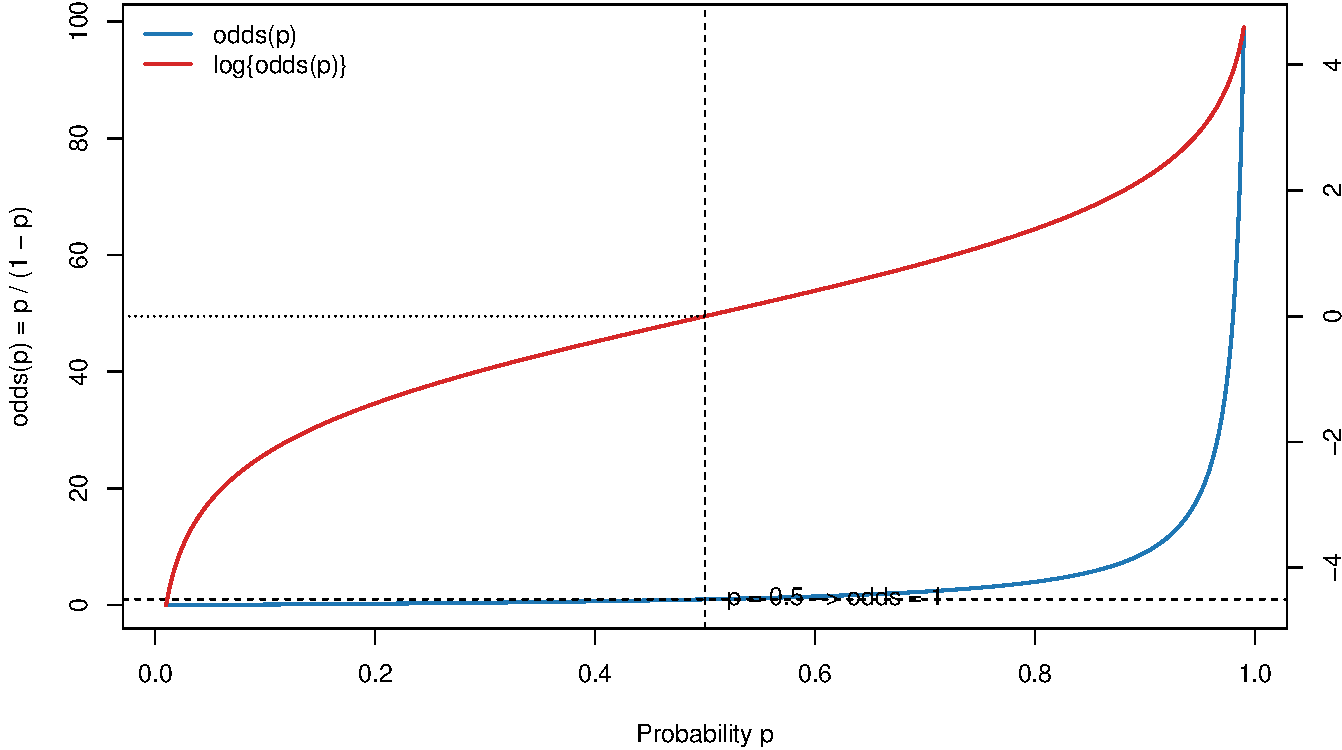
\includegraphics[keepaspectratio]{unit4-lr/logistic_files/figure-pdf/plot-odds-colored-1.pdf}}

Logistic regression models \textbf{log-odds} linearly in predictors,
which both keeps fitted probabilities in ((0,1)) and turns
multiplicative effects on odds into \textbf{additive} effects on the
linear predictor.

\begin{center}\rule{0.5\linewidth}{0.5pt}\end{center}

\section{A Simulated Data}\label{a-simulated-data}

We simulate data from a logistic model where the \textbf{logit} is a
linear function of \(x\):

\[
\operatorname{logit}{p(x)}
=
\log\left(\frac{p(x)}{1-p(x)}\right)
=
\beta_0 + \beta_1 x,
\]

so that

\[
p(x)
=
\operatorname{logit}^{-1}(\beta_0+\beta_1 x)
=
\frac{1}{1+\exp{-(\beta_0+\beta_1 x)}}.
\]

We then display the observed \(y_i\) (binary outcomes) and the true
probability curve \(p(x)\) in red.

\begin{Shaded}
\begin{Highlighting}[]
\FunctionTok{set.seed}\NormalTok{(}\DecValTok{123}\NormalTok{)}

\CommentTok{\# {-}{-} Truth (edit as desired) {-}{-}}
\NormalTok{n     }\OtherTok{\textless{}{-}} \DecValTok{200}
\NormalTok{beta0 }\OtherTok{\textless{}{-}} \DecValTok{0}
\NormalTok{beta1 }\OtherTok{\textless{}{-}}  \DecValTok{4}

\CommentTok{\# {-}{-} Simulate {-}{-}}
\NormalTok{x   }\OtherTok{\textless{}{-}} \FunctionTok{runif}\NormalTok{(n, }\SpecialCharTok{{-}}\DecValTok{1}\NormalTok{, }\DecValTok{1}\NormalTok{)             }\CommentTok{\# predictor}
\NormalTok{eta }\OtherTok{\textless{}{-}}\NormalTok{ beta0 }\SpecialCharTok{+}\NormalTok{ beta1 }\SpecialCharTok{*}\NormalTok{ x}
\NormalTok{p   }\OtherTok{\textless{}{-}} \FunctionTok{plogis}\NormalTok{(eta)                 }\CommentTok{\# true p(x)}
\NormalTok{y   }\OtherTok{\textless{}{-}} \FunctionTok{rbinom}\NormalTok{(n, }\AttributeTok{size =} \DecValTok{1}\NormalTok{, }\AttributeTok{prob =}\NormalTok{ p) }\CommentTok{\# outcomes}

\NormalTok{sim.data }\OtherTok{\textless{}{-}} \FunctionTok{data.frame}\NormalTok{(}\AttributeTok{x =}\NormalTok{ x, }\AttributeTok{y =}\NormalTok{ y, }\AttributeTok{p =}\NormalTok{ p)}
\end{Highlighting}
\end{Shaded}

\subsection{Fit a logistic model to the simulated
data}\label{fit-a-logistic-model-to-the-simulated-data}

\begin{Shaded}
\begin{Highlighting}[]
\CommentTok{\# {-}{-} Optional: fit a model to the simulated data {-}{-}}
\NormalTok{sim.fit }\OtherTok{\textless{}{-}} \FunctionTok{glm}\NormalTok{(y }\SpecialCharTok{\textasciitilde{}}\NormalTok{ x, }\AttributeTok{data =}\NormalTok{ sim.data, }\AttributeTok{family =} \FunctionTok{binomial}\NormalTok{())}
\NormalTok{p\_fit }\OtherTok{\textless{}{-}} \FunctionTok{predict}\NormalTok{(sim.fit, }\AttributeTok{newdata =} \FunctionTok{data.frame}\NormalTok{(}\AttributeTok{x =}\NormalTok{ x), }\AttributeTok{type =} \StringTok{"response"}\NormalTok{)}

\CommentTok{\# {-}{-} Plot: points for y\_i (jittered), red line for true p(x) {-}{-}}
\CommentTok{\# Define jitter amount}
\NormalTok{jit }\OtherTok{\textless{}{-}} \FloatTok{0.05} 
\CommentTok{\# jitter to separate 0/1 visually}
\NormalTok{yj }\OtherTok{\textless{}{-}} \FunctionTok{jitter}\NormalTok{(sim.data}\SpecialCharTok{$}\NormalTok{y, }\AttributeTok{amount =}\NormalTok{ jit) }

\FunctionTok{plot}\NormalTok{(sim.data}\SpecialCharTok{$}\NormalTok{x, yj,}
     \AttributeTok{pch =} \DecValTok{16}\NormalTok{, }\AttributeTok{col =} \FunctionTok{rgb}\NormalTok{(}\DecValTok{0}\NormalTok{, }\DecValTok{0}\NormalTok{, }\DecValTok{0}\NormalTok{, }\FloatTok{0.45}\NormalTok{),}
     \AttributeTok{xlab =} \StringTok{"x"}\NormalTok{,}
     \AttributeTok{ylab =} \StringTok{"Observed y (points) \& p(x) (curves)"}\NormalTok{,}
     \AttributeTok{ylim =} \FunctionTok{c}\NormalTok{(}\SpecialCharTok{{-}}\FloatTok{0.1}\NormalTok{, }\FloatTok{1.1}\NormalTok{))}

\CommentTok{\# True probability curve (red)}
\NormalTok{xg }\OtherTok{\textless{}{-}} \FunctionTok{seq}\NormalTok{(}\FunctionTok{min}\NormalTok{(x), }\FunctionTok{max}\NormalTok{(x), }\AttributeTok{length.out =} \DecValTok{500}\NormalTok{)}
\FunctionTok{lines}\NormalTok{(xg, }\FunctionTok{plogis}\NormalTok{(beta0 }\SpecialCharTok{+}\NormalTok{ beta1 }\SpecialCharTok{*}\NormalTok{ xg), }\AttributeTok{col =} \StringTok{"red"}\NormalTok{, }\AttributeTok{lwd =} \DecValTok{2}\NormalTok{)}

\CommentTok{\# Optional: add fitted probability curve (dashed dark red)}
\FunctionTok{lines}\NormalTok{(xg, }\FunctionTok{predict}\NormalTok{(sim.fit, }\AttributeTok{newdata =} \FunctionTok{data.frame}\NormalTok{(}\AttributeTok{x =}\NormalTok{ xg), }\AttributeTok{type =} \StringTok{"response"}\NormalTok{),}
      \AttributeTok{col =} \StringTok{"darkred"}\NormalTok{, }\AttributeTok{lwd =} \DecValTok{2}\NormalTok{, }\AttributeTok{lty =} \DecValTok{2}\NormalTok{)}

\FunctionTok{legend}\NormalTok{(}\StringTok{"topleft"}\NormalTok{,}
       \AttributeTok{legend =} \FunctionTok{c}\NormalTok{(}\StringTok{"y (jittered points)"}\NormalTok{, }\StringTok{"true p(x)"}\NormalTok{, }\StringTok{"fitted p(x)"}\NormalTok{),}
       \AttributeTok{pch    =} \FunctionTok{c}\NormalTok{(}\DecValTok{16}\NormalTok{, }\ConstantTok{NA}\NormalTok{, }\ConstantTok{NA}\NormalTok{),}
       \AttributeTok{lty    =} \FunctionTok{c}\NormalTok{(}\ConstantTok{NA}\NormalTok{, }\DecValTok{1}\NormalTok{, }\DecValTok{2}\NormalTok{),}
       \AttributeTok{col    =} \FunctionTok{c}\NormalTok{(}\FunctionTok{rgb}\NormalTok{(}\DecValTok{0}\NormalTok{,}\DecValTok{0}\NormalTok{,}\DecValTok{0}\NormalTok{,}\FloatTok{0.45}\NormalTok{), }\StringTok{"red"}\NormalTok{, }\StringTok{"darkred"}\NormalTok{),}
       \AttributeTok{lwd    =} \FunctionTok{c}\NormalTok{(}\ConstantTok{NA}\NormalTok{, }\DecValTok{2}\NormalTok{, }\DecValTok{2}\NormalTok{),}
       \AttributeTok{bty    =} \StringTok{"n"}\NormalTok{)}
\end{Highlighting}
\end{Shaded}

\pandocbounded{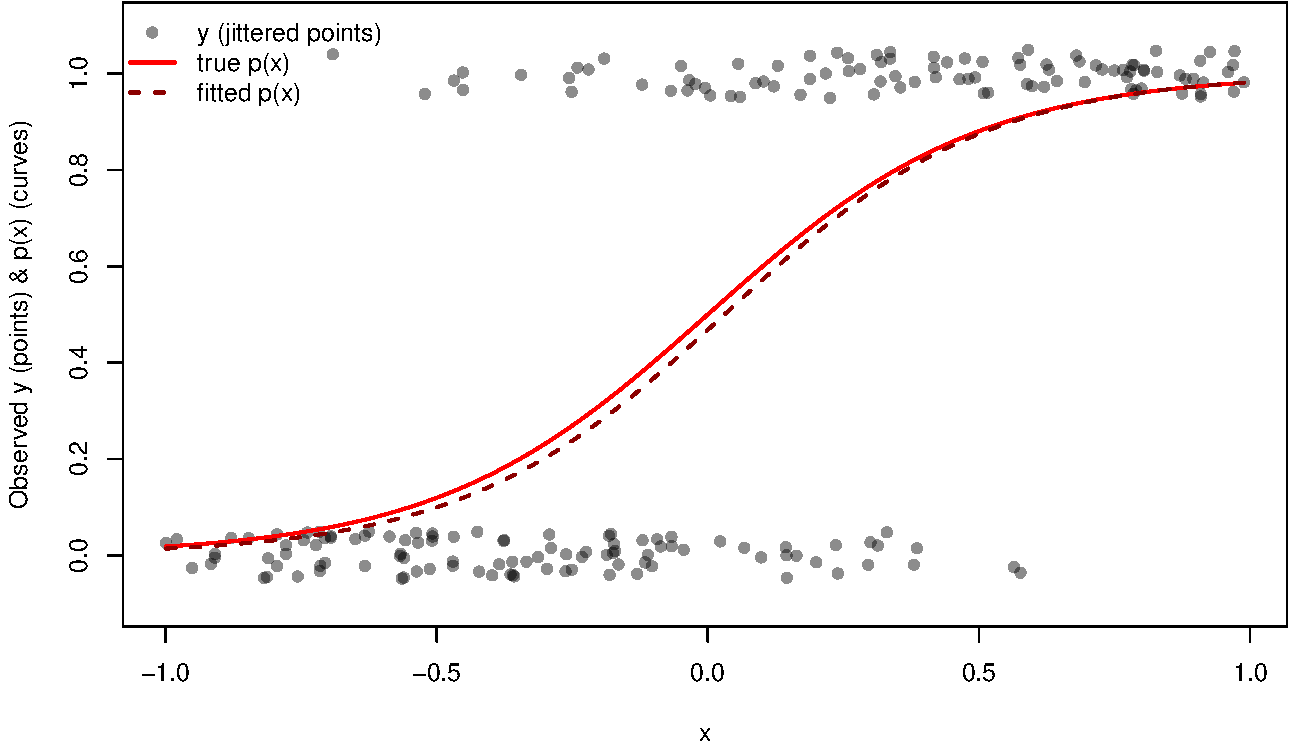
\includegraphics[keepaspectratio]{unit4-lr/logistic_files/figure-pdf/unnamed-chunk-2-1.pdf}}

\section{Example of Coronary Heart Disease
Data}\label{example-of-coronary-heart-disease-data}

\subsection{Load a dataset}\label{load-a-dataset}

This dataset is about a follow-up study to determine the development of
coronary heart disease (CHD) over 9 years of follow-up of 609 white
males from Evans County, Georgia.

\textbf{Variable meanings (as provided):}

\begin{itemize}
\tightlist
\item
  \texttt{chd}: 1 if a person has the disease, 0 otherwise.
\item
  \texttt{smk}: 1 if smoker, 0 if not.
\item
  \texttt{cat}: 1 if catecholamine level is high, 0 if low.
\item
  \texttt{sbp}: systolic blood pressure (continuous).
\item
  \texttt{age}: age in years (continuous).
\item
  \texttt{chl}: cholesterol level (continuous).
\item
  \texttt{ecg}: 1 if electrocardiogram is abnormal, 0 if normal.
\item
  \texttt{hpt}: 1 if high blood pressure, 0 if normal.
\end{itemize}

\begin{Shaded}
\begin{Highlighting}[]
\CommentTok{\# Adjust the path if needed. The default is your original V: drive path.}
\NormalTok{data\_path }\OtherTok{\textless{}{-}} \StringTok{"evans.dat"}

\CommentTok{\# Read data (expects a header row)}
\NormalTok{CHD.data }\OtherTok{\textless{}{-}} \FunctionTok{read.table}\NormalTok{(data\_path, }\AttributeTok{header =} \ConstantTok{TRUE}\NormalTok{)}

\NormalTok{CHD.data}
\end{Highlighting}
\end{Shaded}

\begin{verbatim}
       id chd age cat chl dbp ecg sbp smk hpt
1      21   0  56   0 270  80   0 138   0   0
2      31   0  43   0 159  74   0 128   1   0
3      51   1  56   1 201 112   1 164   1   1
4      71   0  64   1 179 100   0 200   1   1
5      74   0  49   0 243  82   0 145   1   0
6      91   0  46   0 252  88   0 142   1   0
7     111   1  52   0 179  80   1 128   1   0
8     131   0  63   0 217  92   0 135   0   0
9     141   0  42   0 176  76   0 114   1   0
10    191   0  55   0 250 114   1 182   0   1
11    201   0  74   0 293 100   0 166   0   1
12    241   0  53   0 179  90   0 158   0   0
13    251   0  58   0 201  86   0 142   1   0
14    261   0  56   0 206  85   0 120   1   0
15    271   0  69   0 225  84   0 168   0   1
16    283   1  51   1 259 102   1 135   0   1
17    291   0  43   0 193  78   0 118   1   0
18    311   0  64   1 185 100   1 180   0   1
19    312   0  44   0 150 108   0 160   0   1
20    331   0  42   0 211  86   1 122   0   0
21    351   0  57   0 216  88   0 130   0   0
22    381   1  64   1 247  75   1 130   0   0
23    401   0  49   0 200  82   0 130   0   0
24    411   0  68   1 205  74   0 152   1   0
25    431   0  41   0 225  98   0 135   1   1
26    441   0  64   0 263  98   0 162   1   1
27    451   0  41   0 205  80   0 120   0   0
28    481   0  59   0 253  98   0 154   0   1
29    501   0  50   0 282  90   0 142   1   0
30    521   0  56   0 230  80   0 118   0   0
31    541   0  57   1 203 112   0 182   0   1
32    561   0  42   0 211  86   0 144   0   0
33    571   0  59   0 234  84   0 164   1   1
34    581   0  44   0 202  94   1 174   1   1
35    611   0  52   0 162  78   0 134   1   0
36    621   0  45   0 191  85   0 135   0   0
37    641   0  41   0 220 110   0 178   0   1
38    651   0  59   0 240  80   0 130   0   0
39    671   0  52   0 189 110   0 168   0   1
40    681   0  64   0 247 102   0 170   0   1
41    731   0  46   0 181 122   1 176   1   1
42    741   0  42   0 168  75   0 104   1   0
43    751   0  54   0 187  86   0 146   1   0
44    761   0  48   0 196  98   0 130   0   1
45    811   0  45   0 155  70   0 142   1   0
46    851   0  66   1 173 100   0 160   1   1
47    861   0  41   0 138  70   0 115   1   0
48    871   0  76   0 269  94   0 175   1   1
49    881   1  49   0 266 102   0 152   1   1
50    921   0  57   1 200 100   0 160   1   1
51    941   0  51   0 188  84   0 124   1   0
52    961   1  43   0 218 108   1 136   1   1
53    971   0  43   0 212  80   1 108   1   0
54    981   0  45   0 212 102   0 150   1   1
55    991   0  45   0 180  80   0 122   1   0
56   1061   1  46   1 166  76   1 162   0   1
57   1071   0  40   0 257  84   0 130   0   0
58   1081   0  48   0 243  82   1 154   1   0
59   1091   0  64   1 179 100   1 148   1   1
60   1111   0  70   0 167  64   0 112   1   0
61   1151   0  52   0 178  84   1 112   1   0
62   1171   0  55   0 178  94   0 152   0   0
63   1181   0  49   0 211  68   0 114   1   0
64   1191   1  56   0 171  85   0 125   1   0
65   1201   1  66   1 205  80   0 150   1   0
66   1221   0  48   0 229 130   0 195   1   1
67   1231   0  47   0 238 120   1 160   1   1
68   1471   0  54   1 195 112   0 174   1   1
69   1501   0  44   0 162  82   0 120   0   0
70   1561   0  51   0 240  84   1 126   1   0
71   1691   0  43   0 177 102   1 138   1   1
72   1701   0  68   0 252  88   1 112   1   0
73   1741   0  49   0 217 105   0 148   0   1
74   1751   0  55   0 263  84   0 114   0   0
75   1761   0  51   0 229 100   0 162   1   1
76   1791   0  50   0 245  96   0 144   0   1
77   1811   0  65   0 177  74   0 122   0   0
78   1821   0  42   0 203  78   0 134   1   0
79   1851   0  57   0 194  75   1 114   0   0
80   1881   0  42   0 288 110   0 142   0   1
81   1891   0  53   0 217  70   0 120   1   0
82   1901   0  57   1 163  94   0 184   0   1
83   1911   0  61   0 180  84   0 136   0   0
84   1951   0  53   0 209  98   0 142   1   1
85   1961   0  45   0 200  80   0 135   0   0
86   1971   0  44   0 194  80   0 120   1   0
87   2241   0  63   0 227  90   1 135   0   0
88   2252   0  42   0 158  92   0 135   1   0
89   2273   0  73   1 183 120   1 220   0   1
90   2281   0  47   0 253 110   0 140   1   1
91   2311   0  56   0 198  88   0 122   1   0
92   2371   1  41   0 228 132   0 162   1   1
93   2381   0  58   0 217  86   0 140   0   0
94   2391   0  55   0 163  70   0 110   1   0
95   2401   0  46   0 212 124   0 184   1   1
96   2461   0  57   0 144  95   0 130   0   1
97   2481   0  44   0 134  74   0 114   1   0
98   2501   0  52   1 183  96   0 158   1   1
99   2511   0  56   0 212 108   0 144   0   1
100  2531   0  64   0 214  82   0 128   1   0
101  2541   0  54   0 249  92   0 120   1   0
102  2571   0  52   0 180  78   1 104   1   0
103  2591   0  42   0 212  92   0 125   1   0
104  2611   0  46   0 167  82   0 120   1   0
105  2621   0  46   0 273  94   0 152   0   0
106  2631   0  42   0 210  96   0 134   1   1
107  2641   0  54   1 173 110   0 170   1   1
108  2671   0  43   0 256  72   0 114   1   0
109  2681   0  53   0 234  80   0 122   0   0
110  2691   1  40   0 221 100   0 140   1   1
111  2711   0  46   0 261  86   0 128   1   0
112  2731   0  43   0 299  80   0 116   0   0
113  2851   0  43   0 192  75   0 115   1   0
114  2861   0  47   0 185  80   1 146   1   0
115  2871   0  44   0 283  70   0 108   1   0
116  2881   0  49   0 176  92   0 134   1   0
117  2891   1  56   1 331 110   0 190   1   1
118  2901   1  56   0 203  82   0 120   1   0
119  2911   0  64   1 217  92   0 166   1   1
120  2921   0  54   0 164  72   0 122   1   0
121  2931   0  54   0 256  98   0 148   0   1
122  2991   0  51   0 184  98   0 170   0   1
123  3001   0  49   0 165  80   0 114   1   0
124  3011   0  47   0 189  92   0 145   0   0
125  3031   0  58   0 221  88   0 140   1   0
126  3061   0  70   1 126  66   1 164   1   1
127  3601   0  42   0 169  80   1 122   1   0
128  3611   0  59   0 266  92   0 138   0   0
129  3621   0  57   1 153  92   0 148   1   0
130  3651   0  76   1 211 114   1 228   1   1
131  3661   0  43   0 113  76   0 114   1   0
132  3701   0  46   0 200  85   0 145   1   0
133  3721   0  75   1 172 114   1 162   1   1
134  3751   0  42   0 131  84   0 130   0   0
135  3761   0  64   0 214  84   0 120   0   0
136  3771   0  63   1 236  94   1 190   0   1
137  3791   0  54   0 213  90   0 142   0   0
138  3811   0  66   0 226  90   0 166   0   1
139  3813   0  44   0 200 110   0 160   1   1
140  3841   0  72   0 188  78   0 130   0   0
141  3861   0  50   0 268 102   0 138   0   1
142  3871   0  59   1 195 114   1 208   0   1
143  3881   1  59   0 216  95   0 140   1   1
144  3891   0  53   0 182  92   0 130   1   0
145  3901   0  48   0 178  95   0 135   1   1
146  3911   0  40   0 191  76   0 152   1   0
147  3941   0  61   0 255  80   0 120   0   0
148  3951   0  42   0 225  80   0 126   1   0
149  4161   0  42   0 166  90   0 145   0   0
150  4191   0  49   0 278  84   0 126   1   0
151  4202   0  40   0 235  72   0 116   0   0
152  4221   0  51   0 251  86   0 128   1   0
153  4242   0  44   0 217  90   0 146   0   0
154  4261   0  44   0 181  94   0 144   1   0
155  4271   0  47   0 208 108   0 178   0   1
156  4291   0  51   0 182 112   0 182   0   1
157  4301   0  69   0 228  75   0 115   1   0
158  4321   0  58   1 170  88   1 152   1   0
159  4331   0  74   1 147  80   1 200   0   1
160  4341   0  48   0 190  78   0 114   1   0
161  4381   0  64   0 205  98   1 140   0   1
162  4401   0  53   0 216  78   0 124   1   0
163  4411   0  71   0 170  90   0 140   1   0
164  4421   0  47   0 127  74   0 110   1   0
165  4451   0  56   0 235  92   0 128   1   0
166  4461   0  40   0 200  72   0 118   0   0
167  4491   0  46   0 283 100   0 148   1   1
168  4531   0  68   1 157  94   0 162   0   1
169  4551   1  54   0 206  76   1 142   0   0
170  4581   0  54   0 197  88   0 125   1   0
171  4591   0  45   0 163  75   0 115   1   0
172  4601   0  66   0 176  60   1 124   0   0
173  4641   0  58   0 211  88   0 146   1   0
174  4681   0  49   0 161  75   0 115   0   0
175  4711   0  51   0 244  90   0 128   0   0
176  4731   0  44   0 172 100   0 138   0   1
177  4751   0  61   1 166  86   0 156   1   0
178  4771   0  48   0 184  76   0 116   1   0
179  4781   0  63   0 143  92   0 122   1   0
180  4791   0  54   0 196  84   0 138   1   0
181  4801   0  52   0 189  88   0 142   1   0
182  4811   0  45   0 227  98   1 140   1   1
183  4821   0  62   0 236  94   0 160   0   1
184  4831   0  41   0 240  86   0 144   0   0
185  4851   0  41   0 256  90   0 145   1   0
186  4861   0  61   0 200  84   0 148   1   0
187  4871   0  42   0 199 104   0 166   1   1
188  4901   0  42   0 161  88   0 124   0   0
189  4911   0  72   0 211  80   1 104   0   0
190  4951   0  43   0 180  64   0  92   0   0
191  4961   1  72   0 200  86   1 138   0   0
192  4971   0  51   0 206  80   0 132   1   0
193  4981   0  58   0 254  94   0 152   1   0
194  5011   0  41   0 215  90   0 142   1   0
195  5061   0  71   1 162  98   1 184   1   1
196  5071   1  63   0 145  96   0 162   1   1
197  5091   0  44   0 220  90   1 130   1   0
198  5101   0  45   0 298 108   0 170   1   1
199  5111   0  54   0 300  94   0 148   1   0
200  5131   1  52   1 306 108   0 178   1   1
201  5141   0  55   0 302 134   1 206   1   1
202  5181   1  41   0 158  80   0 140   1   0
203  5191   0  54   0 194 130   1 170   1   1
204  5211   0  64   1 229  94   1 156   1   0
205  5251   0  61   0 259  82   0 118   0   0
206  5281   0  40   0 214  94   0 130   0   0
207  5301   0  51   0 168 106   0 156   1   1
208  5361   0  51   0 265  90   0 158   1   0
209  5391   0  75   0 225  80   0 125   0   0
210  5421   1  40   0 219  80   0 115   1   0
211  5451   1  63   0 202 110   0 160   0   1
212  5461   0  42   1 217  94   1 138   0   0
213  5471   1  64   0 231  85   0 120   1   0
214  5521   1  50   0 215 114   0 170   1   1
215  5601   0  49   0 146  98   1 145   1   1
216  5621   0  48   0 198  75   0 120   1   0
217  5631   0  58   0 206  92   0 154   0   0
218  5641   0  46   0 227  98   0 168   1   1
219  5671   0  46   0 214  92   1 166   1   1
220  6341   0  42   0 225 100   1 162   1   1
221  6351   0  57   0 193  86   0 124   0   0
222  6371   0  50   0 186 102   0 160   0   1
223  6391   0  46   0 147  85   0 122   1   0
224  6411   0  45   0 205 100   0 166   0   1
225  6421   0  57   1 196  98   1 196   1   1
226  6441   0  46   0 195  96   0 138   0   1
227  6451   0  45   1 153 108   1 212   1   1
228  6461   0  58   1 172  96   1 168   0   1
229  6482   0  42   0 293 110   0 176   1   1
230  6491   0  53   0 274 106   0 158   1   1
231  6501   0  55   0 221 106   0 162   0   1
232  6511   0  53   0 197  70   0 112   0   0
233  6531   0  69   1 194 100   1 150   0   1
234  6551   0  58   0 204  74   0 122   1   0
235  6561   0  46   0 203  84   0 114   1   0
236  6591   0  62   0 293  90   1 142   1   0
237  6631   0  61   0 197  72   1 110   0   0
238  6641   0  49   0 195  82   0 138   1   0
239  6651   0  48   0 184  96   0 144   1   1
240  6661   1  55   0 209  85   0 130   1   0
241  6681   0  52   1 209  98   1 170   0   1
242  6691   0  61   0 214 100   0 158   0   1
243  6721   0  68   1 130 106   1 200   0   1
244  6731   0  55   0 196  70   0 125   0   0
245  6741   0  52   1 237 126   1 224   0   1
246  6751   0  43   0 185  85   1 140   1   0
247  6761   1  47   0 248 104   1 132   1   1
248  6781   0  57   0 252 106   0 166   0   1
249  6791   0  55   0 198  96   0 144   1   1
250  6801   0  71   0 176  62   0 138   0   0
251  6811   0  74   1 193  98   1 202   0   1
252  6821   1  65   0 185 105   0 156   0   1
253  6831   0  65   0 241 102   1 146   0   1
254  6871   0  44   0 231  70   0 108   0   0
255  6881   0  40   0 157  78   1 122   0   0
256  6891   0  45   0 152 106   1 148   1   1
257  6911   0  50   0 237 102   0 156   1   1
258  6921   0  64   1 175 110   1 142   0   1
259  6931   1  56   0 195  94   1 150   0   0
260  6941   0  62   1 151  88   0 165   0   1
261  6961   0  44   0 205  80   0 128   1   0
262  6981   0  73   0 190  75   0 115   0   0
263  7001   0  46   0 239 100   0 160   1   1
264  7021   0  51   0 232  80   0 120   0   0
265  7031   0  59   1 170 100   0 180   1   1
266  7051   1  67   1 319 104   0 182   0   1
267  7091   0  54   0 225  86   0 122   0   0
268  7101   0  49   0 252  90   0 128   1   0
269  7121   0  46   0 224  84   0 130   1   0
270  7131   0  42   1 229  90   1 145   0   0
271  8641   0  68   0 195  76   1 116   1   0
272  8651   0  43   0 230  85   1 135   1   0
273  8671   0  56   1 186  98   1 154   0   1
274  8682   0  68   1 192  94   0 154   1   0
275  8711   0  46   0 184  78   0 110   1   0
276  8721   1  64   1 233  94   0 140   1   0
277  8731   0  54   0 175  96   0 156   1   1
278  8751   0  48   0 188 106   0 148   1   1
279  8771   0  41   0 232  82   0 126   1   0
280  8811   0  65   1 178 106   1 194   0   1
281  8841   0  41   0 187 108   0 154   0   1
282  8851   1  42   0 207  86   1 128   1   0
283  8971   0  66   0  94  86   0 134   0   0
284  8981   0  44   0 211  90   0 142   1   0
285  9011   0  42   0 275 100   1 150   1   1
286  9021   0  51   0 165  85   0 130   1   0
287  9031   0  56   0 282  94   0 134   1   0
288  9051   1  64   1 239  94   0 162   1   1
289  9061   0  44   0 256 106   0 162   1   1
290  9071   1  55   0 175 108   0 160   1   1
291  9091   0  55   0 306  82   0 160   1   1
292  9101   1  67   0 188 102   1 168   0   1
293  9191   1  56   1 221  78   1 154   1   0
294  9201   1  63   1 213 156   1 256   0   1
295  9261   1  67   0 250 100   0 158   0   1
296  9471   0  48   0 268 120   0 172   1   1
297  9601   1  45   0 263  86   0 132   0   0
298  9631   0  49   0 150  98   1 120   1   1
299  9651   1  70   1 251 108   1 174   1   1
300  9671   0  45   0 180 102   0 156   1   1
301  9681   0  48   0 336 110   0 174   1   1
302  9711   1  42   0 210  70   0 124   1   0
303  9721   0  69   1 179 110   0 175   1   1
304  9731   0  44   0 177  75   0 120   0   0
305  9751   0  48   0 227  92   0 158   1   0
306  9791   0  46   0 195  72   0 120   1   0
307  9801   0  52   0 227  76   0 116   1   0
308  9811   0  73   0 250  84   0 154   0   0
309  9831   0  67   0 218  96   1 148   0   1
310  9841   0  63   0 229 100   0 168   1   1
311  9871   0  45   1 197  80   1 134   0   0
312  9881   0  46   0 190  86   0 122   1   0
313  9891   0  68   1 189 104   1 202   1   1
314  9901   0  49   0 185  80   0 120   1   0
315  9911   1  63   0 194  90   0 190   1   1
316  9931   0  59   0 192  66   0 134   0   0
317  9941   0  67   1 261  80   1 160   1   1
318  9951   0  49   0 174  78   1 108   0   0
319  9961   0  65   1 189 114   1 168   1   1
320  9981   0  44   0 248 100   0 145   1   1
321 10011   0  45   0 214  94   0 122   0   0
322 10041   0  47   0 275  76   0 114   1   0
323 10051   0  46   0 259  92   0 130   1   0
324 10071   0  52   0 230  68   0 100   0   0
325 10091   0  60   0 206  84   0 138   1   0
326 10121   0  45   0 275  95   0 125   1   1
327 10151   1  67   1 237 100   1 170   1   1
328 10181   0  60   0 289  80   1 118   0   0
329 10201   0  65   1 176  82   0 200   1   1
330 10221   0  72   1 232  80   1 210   1   1
331 10231   1  71   0 184  90   0 160   1   1
332 10241   0  55   0 283 108   1 178   1   1
333 10271   0  54   0 214 110   0 170   1   1
334 10401   0  52   1 161  76   0 162   1   1
335 10402   0  48   0 232  98   0 154   1   1
336 10921   0  66   0 228  72   0 120   1   0
337 10951   0  52   1 206 120   1 206   0   1
338 10971   0  64   0 218  80   0 110   1   0
339 11011   0  42   0 262  92   0 142   1   0
340 11081   0  52   0 227  66   0  98   0   0
341 11101   0  51   0 215  60   0 100   0   0
342 11141   0  54   0 146  70   0 115   0   0
343 11151   0  51   0 268  85   0 140   1   0
344 11161   0  60   0 211  94   0 166   0   1
345 11221   0  48   0 213  90   1 145   1   0
346 11281   0  73   0 249 108   0 206   1   1
347 11291   0  50   0 218  92   0 130   1   0
348 11321   0  45   0 221  92   0 128   0   0
349 11341   1  56   1 228  92   0 152   1   0
350 11351   1  46   0 240 104   0 142   1   1
351 11361   1  76   1 279  96   0 136   1   1
352 11391   0  52   0 186  70   0 118   0   0
353 11441   0  54   0 160 110   1 200   1   1
354 11461   0  53   1 222 104   1 154   0   1
355 11481   0  43   0 211  65   0 112   1   0
356 11491   0  46   0 195 132   1 230   1   1
357 11501   0  63   0 290  90   0 150   0   0
358 11511   0  44   0 220  95   0 138   0   1
359 11531   0  42   0 161  80   0 124   1   0
360 11553   0  74   1 212  98   0 164   1   1
361 11611   0  53   0 182  86   0 136   1   0
362 11651   0  56   1 223 110   1 208   1   1
363 11661   0  47   0 290  92   0 136   1   0
364 11711   0  43   0 249  90   1 162   1   1
365 11721   0  51   0 174  92   0 124   1   0
366 11731   0  63   1 204  92   1 190   1   1
367 11781   0  49   0 245  62   0 124   1   0
368 11791   0  57   1 216 114   0 174   1   1
369 11811   0  43   0 245 120   1 145   0   1
370 11831   0  58   0 151  98   0 138   1   1
371 11851   0  49   1 178 102   0 166   1   1
372 11891   0  47   0 227  88   0 132   1   0
373 11911   0  45   0 253 104   0 152   1   1
374 11941   1  65   1 222  88   1 162   0   1
375 11971   0  51   0 258  94   1 178   1   1
376 11981   0  49   0 182  84   1 124   1   0
377 11991   0  51   0 184  96   0 150   1   1
378 12051   1  67   0 357  90   0 129   0   0
379 12111   0  47   0 193  90   0 135   1   0
380 12121   0  50   0 198  82   1 136   1   0
381 12141   0  48   0 263  76   0 102   0   0
382 12151   0  48   0 254  74   0 124   0   0
383 12181   0  64   0 248  74   0 126   1   0
384 12221   0  43   0 197  84   0 122   1   0
385 12231   0  41   0 282  98   0 132   0   1
386 12241   0  48   0 238 106   0 144   1   1
387 12251   0  50   0 156  74   0 122   1   0
388 12271   0  46   0 234  70   0 120   1   0
389 12281   0  44   0 203  82   0 110   1   0
390 12291   1  65   0 200  90   0 160   1   1
391 12293   0  44   0 209  84   0 132   1   0
392 12311   0  40   0 245  94   0 142   0   0
393 12351   0  56   0 124  86   0 142   0   0
394 12371   0  56   1 199  86   1 154   1   0
395 12381   1  47   0 148  85   1 145   1   0
396 12391   0  48   0 246  92   0 122   1   0
397 12401   0  46   0 233  96   0 138   0   1
398 12431   0  48   0 265 100   1 142   1   1
399 12461   0  50   0 207  86   1 142   1   0
400 12471   0  69   0 227  72   1 108   1   0
401 12481   0  45   0 205 130   1 182   1   1
402 12641   0  57   0 189 102   1 128   1   1
403 12681   1  69   0 191 102   0 164   1   1
404 12741   0  45   0 171  91   0 145   1   0
405 12742   0  52   0 178  91   1 145   1   0
406 12751   0  63   0 229  94   0 148   1   0
407 12761   0  61   1 169  90   0 140   1   0
408 12801   0  48   0 238  88   0 134   1   0
409 12831   1  45   0 216  94   0 138   1   0
410 12861   0  66   1 178 110   0 198   0   1
411 12891   0  54   0 173  92   0 162   0   1
412 12901   0  45   0 173  64   0 120   1   0
413 12911   1  66   0 180 104   1 162   1   1
414 12921   0  53   0 168 110   0 154   1   1
415 12941   0  40   0 277  80   0 120   0   0
416 13021   0  55   0 181  78   0 132   1   0
417 13041   0  48   0 272  98   1 156   1   1
418 13051   0  49   0 307  88   0 130   0   0
419 13101   0  61   0 203  94   1 146   0   0
420 13111   0  41   0 212  90   0 120   1   0
421 13121   0  43   0 248 118   0 142   1   1
422 13131   0  47   0 208 110   0 160   1   1
423 13321   0  46   0 218  86   0 126   1   0
424 13351   0  63   1 163  76   0 175   1   1
425 13391   0  62   0 261  88   0 130   1   0
426 13421   0  72   0 224 100   1 190   0   1
427 13431   0  50   0 292  80   1 128   1   0
428 13451   0  46   0 202 100   1 172   1   1
429 13461   0  44   0 145  72   0 114   1   0
430 13471   0  46   1 183  88   1 162   1   1
431 13481   0  47   0 188  88   0 126   1   0
432 13511   0  51   1 209 106   0 180   1   1
433 13521   0  46   0 217  84   0 144   1   0
434 13531   0  47   0 180  78   0 126   1   0
435 13541   0  44   0 190  90   0 140   0   0
436 13551   0  55   0 211  80   0 115   1   0
437 13571   0  56   0 204  76   0 124   1   0
438 13591   0  54   0 185  98   0 170   0   1
439 13611   1  50   0 206  70   0 108   1   0
440 13641   0  59   0 265  96   0 150   1   1
441 13651   0  47   0 246  80   0 130   0   0
442 13661   0  65   1 171 102   0 166   0   1
443 13662   0  41   0 211  91   0 145   0   0
444 13671   0  47   0 139  96   1 192   1   1
445 13691   0  49   0 155  84   0 124   0   0
446 13721   0  50   0 229  90   0 134   0   0
447 13731   0  56   1 148 110   0 168   1   1
448 13751   0  50   0 198  86   0 134   1   0
449 13761   0  55   1 186 120   0 172   1   1
450 13771   0  52   0 211  70   0 112   1   0
451 13811   0  57   0 210  80   0 120   1   0
452 13841   1  47   1 212 122   1 220   1   1
453 13861   0  59   0 227  70   0 122   0   0
454 13901   0  47   0 232  90   0 142   0   0
455 13911   0  42   0 176  88   0 122   1   0
456 13931   0  56   0 166  86   0 126   0   0
457 13941   1  43   0 268  88   1 132   1   0
458 13951   0  55   0 178  80   0 104   1   0
459 13961   0  49   1 147 134   1 300   1   1
460 13971   0  71   1 164  94   0 174   0   1
461 14041   0  71   1 187 114   1 172   0   1
462 14071   0  69   1 165  96   1 140   0   1
463 14691   0  47   0 250  88   1 122   1   0
464 14701   0  44   0 199  70   0 120   1   0
465 14711   1  65   1 233 116   1 180   1   1
466 14731   0  65   0 182  74   0 124   0   0
467 14741   0  40   0 210  94   0 128   0   0
468 14751   0  47   0 235  86   0 128   1   0
469 14761   0  54   0 172  92   0 144   1   0
470 14771   0  64   1 198 100   0 178   0   1
471 14781   0  59   1 212  90   1 198   0   1
472 14801   0  72   0 285  90   1 150   1   0
473 14811   0  52   0 194  82   0 132   0   0
474 14861   0  56   0 237  70   0 106   0   0
475 14871   0  56   0 153  66   1  96   0   0
476 14881   0  54   0 219  92   0 152   1   0
477 14901   0  60   1 188 114   1 210   1   1
478 14911   0  63   0 276  95   1 145   0   1
479 14931   0  73   0 203  68   0 130   1   0
480 14941   1  49   0 228  98   0 140   1   1
481 14981   0  57   0 199  80   0 134   0   0
482 15001   0  53   1 162  90   0 158   1   0
483 15011   0  43   0 221  94   0 125   1   0
484 15021   0  68   0 150  78   0 145   0   0
485 15031   0  53   0 140  80   0 120   1   0
486 15041   0  50   0 162  65   1 110   0   0
487 15061   0  49   0 171  86   1 125   1   0
488 15091   0  62   0 206  94   0 144   0   0
489 15111   0  52   0 226  76   0 130   1   0
490 15121   0  57   1 113  94   1 146   1   0
491 15141   0  45   0 197  78   0 118   0   0
492 15161   0  50   0 180  88   0 132   1   0
493 15171   0  50   1 180 118   1 214   1   1
494 15191   0  53   0 196  86   0 144   1   0
495 15201   0  51   0 211  98   0 135   0   1
496 15211   0  58   1 164  96   1 155   1   1
497 15221   0  64   0 218  85   0 154   0   0
498 15251   1  49   0 191  76   0 132   1   0
499 15271   0  55   0 189  64   0 110   0   0
500 15311   0  50   0 156  82   0 114   1   0
501 15321   0  50   0 223  80   0 130   1   0
502 15361   0  57   0 165  76   0 132   1   0
503 15401   0  55   1 200  94   1 188   1   1
504 15421   0  48   1 162 135   1 250   1   1
505 15431   0  56   1 207 110   0 172   1   1
506 15441   0  72   0 262  84   0 172   1   1
507 15511   1  67   1 236 106   1 200   0   1
508 15541   0  70   1 192  90   1 162   0   1
509 15562   0  57   1 203 100   0 170   1   1
510 15611   0  67   1 200 160   1 224   0   1
511 15641   0  62   0 280  86   0 124   1   0
512 15651   0  72   1 229 140   1 270   1   1
513 15661   0  70   0 290  84   0 138   0   0
514 15671   0  65   0 222  88   0 146   0   0
515 15691   0  58   0 259 100   1 154   0   1
516 15711   0  64   0 205  80   0 140   0   0
517 15761   0  44   0 276  74   0 112   1   0
518 15791   0  55   0 171  68   0 110   0   0
519 15831   0  71   0 287  90   0 130   0   0
520 15851   1  72   0 174  78   1 192   1   1
521 15882   0  71   0 277 110   1 200   0   1
522 15891   0  54   0 192  85   0 130   0   0
523 15911   0  51   0 196  90   0 128   1   0
524 15921   0  68   0 203  74   0 138   1   0
525 15931   0  47   0 271  85   0 145   1   0
526 15941   0  49   1 169  85   1 145   0   0
527 15951   0  48   0 201  98   0 150   1   1
528 15981   0  74   0 244  94   0 164   0   1
529 15991   0  49   0 161  92   0 120   0   0
530 16321   1  53   0 192 106   0 164   1   1
531 16431   0  46   0 192  86   1 116   1   0
532 16441   0  59   0 230  84   0 158   1   0
533 16461   0  50   0 312  98   1 138   0   1
534 16481   1  69   1 230 100   1 170   0   1
535 16501   1  75   1 233  90   1 222   1   1
536 16531   0  42   0 207  72   0 106   1   0
537 16541   0  50   0 317  90   1 138   0   0
538 16571   0  44   0 213  84   0 118   1   0
539 16581   0  44   0 220  98   0 140   0   1
540 16591   0  42   0 225  95   0 140   0   1
541 16622   0  42   0 288 104   0 150   1   1
542 16691   0  44   0 168  94   1 134   1   0
543 16701   0  57   1 182  96   1 138   1   1
544 16711   1  68   1 242  84   0 128   1   0
545 16752   0  69   0 258  82   0 145   1   0
546 16761   0  74   1 172 100   0 190   1   1
547 16841   0  56   1 239 140   1 220   1   1
548 16871   1  58   1 209  94   1 140   1   0
549 16891   0  46   0 181  84   0 124   0   0
550 16911   0  60   1 199 100   0 162   0   1
551 16931   0  62   0 217  90   0 144   1   0
552 16971   0  74   0 200  78   0 118   1   0
553 17071   0  44   0 268  80   0 126   1   0
554 17111   0  54   0 202  86   0 134   0   0
555 17121   0  49   0 224  86   1 134   1   0
556 17131   0  46   0 302 102   0 160   1   1
557 17151   0  45   0 239  90   0 128   0   0
558 17161   0  57   0 205  88   0 140   0   0
559 17171   0  56   1 192 170   1 270   0   1
560 17181   0  42   0 282 114   0 170   1   1
561 17191   0  52   0 232  94   0 144   1   0
562 17211   0  49   0 229  92   0 162   1   1
563 17231   0  51   0 336  86   0 130   1   0
564 17251   0  40   0 146  84   0 125   0   0
565 17271   0  43   0 224  72   0 115   0   0
566 17291   0  45   0 228  76   1 136   1   0
567 17361   0  63   0 211 108   0 144   1   1
568 17401   0  52   0 212  76   0 118   0   0
569 17481   1  67   1 243 118   1 220   1   1
570 17961   0  72   1 208  94   1 174   1   1
571 17991   0  54   0 284  98   0 146   1   1
572 18061   0  52   0 190  88   1 130   1   0
573 18071   0  49   0 264  92   0 162   0   1
574 18101   0  42   0 288 108   0 146   0   1
575 18121   0  41   0 181  94   0 136   1   0
576 18131   1  56   1 283 100   0 188   1   1
577 18141   0  46   0 217  66   0 120   1   0
578 18151   1  52   0 250  80   0 132   1   0
579 18161   0  44   0 209  70   0 116   1   0
580 18171   1  43   0 189 106   0 154   1   1
581 18201   0  73   0 190  78   0 138   0   0
582 18401   0  54   0 223  82   0 122   1   0
583 18411   0  46   0 241  84   0 120   1   0
584 18421   0  44   0 214  96   1 142   1   1
585 18441   0  43   0 207  86   0 122   0   0
586 18481   0  46   0 186  86   0 130   0   0
587 18491   1  74   1 212  70   1 144   1   0
588 18511   0  54   1 211  94   1 152   0   0
589 18521   0  63   0 223  86   0 158   1   0
590 18551   0  58   1 206 108   1 192   0   1
591 18581   0  50   0 194  92   0 134   1   0
592 18631   0  71   0 193  82   0 115   1   0
593 18661   0  52   0 213  90   0 140   1   0
594 18681   0  63   0 318  82   1 126   0   0
595 18711   0  66   0 216 104   1 154   0   1
596 18731   0  60   0 211  66   0 128   1   0
597 18752   0  47   0 219  88   0 128   1   0
598 18771   0  57   0 322  98   0 144   1   1
599 18801   0  66   1 239 100   1 184   1   1
600 18841   0  66   1 195 104   0 158   1   1
601 18871   0  47   0 243  78   0 118   1   0
602 18921   0  60   0 223  92   1 122   1   0
603 18971   0  48   0 174 102   0 160   1   1
604 19003   0  61   1 163  86   1 144   1   0
605 19011   0  64   0 225  90   0 160   1   1
606 19061   1  46   0 252 122   0 158   1   1
607 19091   0  49   0 261 102   0 166   1   1
608 19121   0  51   0 184  88   0 118   1   0
609 19161   0  64   0 206  82   0 152   0   0
\end{verbatim}

\begin{Shaded}
\begin{Highlighting}[]
\FunctionTok{colnames}\NormalTok{(CHD.data)}
\end{Highlighting}
\end{Shaded}

\begin{verbatim}
 [1] "id"  "chd" "age" "cat" "chl" "dbp" "ecg" "sbp" "smk" "hpt"
\end{verbatim}

\subsection{Fit Logistic Regression Model for a Single
Variable}\label{fit-logistic-regression-model-for-a-single-variable}

\begin{Shaded}
\begin{Highlighting}[]
\NormalTok{vars }\OtherTok{\textless{}{-}} \FunctionTok{c}\NormalTok{(}\StringTok{"smk"}\NormalTok{, }\StringTok{"sbp"}\NormalTok{, }\StringTok{"age"}\NormalTok{, }\StringTok{"chl"}\NormalTok{)}
\CommentTok{\#jit  \textless{}{-} 0.01  \# global jitter amount for y}

\CommentTok{\# par(mfrow = c(2, 2), mar = c(4, 4, 2, 4) + 0.1)  \# extra right margin for axis(4)}

\ControlFlowTok{for}\NormalTok{ (v }\ControlFlowTok{in}\NormalTok{ vars) \{}
  \CommentTok{\# Univariate logistic regression using ORIGINAL variable name in the formula}
\NormalTok{  fit }\OtherTok{\textless{}{-}} \FunctionTok{glm}\NormalTok{(}
    \AttributeTok{formula =} \FunctionTok{reformulate}\NormalTok{(v, }\AttributeTok{response =} \StringTok{"chd"}\NormalTok{),}
    \AttributeTok{data    =}\NormalTok{ CHD.data,}
    \AttributeTok{family  =} \FunctionTok{binomial}\NormalTok{()}
\NormalTok{  )}
  \FunctionTok{print}\NormalTok{(}\FunctionTok{summary}\NormalTok{(fit))}

  \CommentTok{\# Base scatter of chd with small jitter (left axis: probability scale)}
  \FunctionTok{plot}\NormalTok{(}
\NormalTok{    CHD.data[[v]],}
    \FunctionTok{jitter}\NormalTok{(CHD.data}\SpecialCharTok{$}\NormalTok{chd, }\AttributeTok{amount =}\NormalTok{ jit),}
    \AttributeTok{pch  =} \DecValTok{16}\NormalTok{, }\AttributeTok{col =} \FunctionTok{rgb}\NormalTok{(}\DecValTok{0}\NormalTok{, }\DecValTok{0}\NormalTok{, }\DecValTok{0}\NormalTok{, }\FloatTok{0.45}\NormalTok{),}
    \AttributeTok{xlab =}\NormalTok{ v, }\AttributeTok{ylab =} \StringTok{"chd (jittered)"}\NormalTok{,}
    \AttributeTok{main =} \FunctionTok{paste}\NormalTok{(}\StringTok{"chd vs"}\NormalTok{, v),}
    \AttributeTok{ylim =} \FunctionTok{c}\NormalTok{(}\SpecialCharTok{{-}}\FloatTok{0.1}\NormalTok{, }\FloatTok{1.1}\NormalTok{)}
\NormalTok{  )}

  \CommentTok{\# Fitted π(x) in red (left axis)}
  \ControlFlowTok{if}\NormalTok{ (}\FunctionTok{length}\NormalTok{(}\FunctionTok{unique}\NormalTok{(CHD.data[[v]])) }\SpecialCharTok{==} \DecValTok{2}\NormalTok{) \{}
    \CommentTok{\# binary predictor}
\NormalTok{    xcat }\OtherTok{\textless{}{-}} \FunctionTok{sort}\NormalTok{(}\FunctionTok{unique}\NormalTok{(CHD.data[[v]]))}
\NormalTok{    nd   }\OtherTok{\textless{}{-}} \FunctionTok{setNames}\NormalTok{(}\FunctionTok{data.frame}\NormalTok{(xcat), v)}
\NormalTok{    pcat }\OtherTok{\textless{}{-}} \FunctionTok{predict}\NormalTok{(fit, }\AttributeTok{newdata =}\NormalTok{ nd, }\AttributeTok{type =} \StringTok{"response"}\NormalTok{)}
    \FunctionTok{points}\NormalTok{(xcat, pcat, }\AttributeTok{pch =} \DecValTok{19}\NormalTok{, }\AttributeTok{col =} \StringTok{"red"}\NormalTok{)}
    \FunctionTok{lines}\NormalTok{(xcat, pcat, }\AttributeTok{col =} \StringTok{"red"}\NormalTok{, }\AttributeTok{lwd =} \DecValTok{2}\NormalTok{)}

    \CommentTok{\# Right{-}axis: logit\{π(x)\} with fixed y{-}limits}
\NormalTok{    logit\_p }\OtherTok{\textless{}{-}} \FunctionTok{log}\NormalTok{(pcat }\SpecialCharTok{/}\NormalTok{ (}\DecValTok{1} \SpecialCharTok{{-}}\NormalTok{ pcat))}
    \FunctionTok{par}\NormalTok{(}\AttributeTok{new =} \ConstantTok{TRUE}\NormalTok{)}
    \FunctionTok{plot}\NormalTok{(}
\NormalTok{      xcat, logit\_p, }\AttributeTok{type =} \StringTok{"l"}\NormalTok{, }\AttributeTok{lwd =} \DecValTok{2}\NormalTok{, }\AttributeTok{col =} \StringTok{"blue"}\NormalTok{,}
      \AttributeTok{axes =} \ConstantTok{FALSE}\NormalTok{, }\AttributeTok{xlab =} \StringTok{""}\NormalTok{, }\AttributeTok{ylab =} \StringTok{""}\NormalTok{,}
      \AttributeTok{xlim =} \FunctionTok{range}\NormalTok{(CHD.data[[v]]), }\AttributeTok{ylim =} \FunctionTok{c}\NormalTok{(}\SpecialCharTok{{-}}\FloatTok{2.5}\NormalTok{, }\DecValTok{0}\NormalTok{)}
\NormalTok{    )}
    \FunctionTok{axis}\NormalTok{(}\DecValTok{4}\NormalTok{)}
    \FunctionTok{mtext}\NormalTok{(}\StringTok{"logit(p(x))"}\NormalTok{, }\AttributeTok{side =} \DecValTok{4}\NormalTok{, }\AttributeTok{line =} \DecValTok{3}\NormalTok{)}
    \FunctionTok{par}\NormalTok{(}\AttributeTok{new =} \ConstantTok{FALSE}\NormalTok{)}

\NormalTok{  \} }\ControlFlowTok{else}\NormalTok{ \{}
    \CommentTok{\# continuous predictor}
\NormalTok{    xg }\OtherTok{\textless{}{-}} \FunctionTok{seq}\NormalTok{(}\FunctionTok{min}\NormalTok{(CHD.data[[v]]), }\FunctionTok{max}\NormalTok{(CHD.data[[v]]), }\AttributeTok{length.out =} \DecValTok{400}\NormalTok{)}
\NormalTok{    nd }\OtherTok{\textless{}{-}} \FunctionTok{setNames}\NormalTok{(}\FunctionTok{data.frame}\NormalTok{(xg), v)}
\NormalTok{    pg }\OtherTok{\textless{}{-}} \FunctionTok{predict}\NormalTok{(fit, }\AttributeTok{newdata =}\NormalTok{ nd, }\AttributeTok{type =} \StringTok{"response"}\NormalTok{)}
    \FunctionTok{lines}\NormalTok{(xg, pg, }\AttributeTok{col =} \StringTok{"red"}\NormalTok{, }\AttributeTok{lwd =} \DecValTok{2}\NormalTok{)}

    \CommentTok{\# Right{-}axis: logit\{π(x)\} with fixed y{-}limits}
\NormalTok{    logit\_pg }\OtherTok{\textless{}{-}} \FunctionTok{log}\NormalTok{(pg }\SpecialCharTok{/}\NormalTok{ (}\DecValTok{1} \SpecialCharTok{{-}}\NormalTok{ pg))}
    \FunctionTok{par}\NormalTok{(}\AttributeTok{new =} \ConstantTok{TRUE}\NormalTok{)}
    \FunctionTok{plot}\NormalTok{(}
\NormalTok{      xg, logit\_pg, }\AttributeTok{type =} \StringTok{"l"}\NormalTok{, }\AttributeTok{lwd =} \DecValTok{2}\NormalTok{, }\AttributeTok{col =} \StringTok{"blue"}\NormalTok{,}
      \AttributeTok{axes =} \ConstantTok{FALSE}\NormalTok{, }\AttributeTok{xlab =} \StringTok{""}\NormalTok{, }\AttributeTok{ylab =} \StringTok{""}\NormalTok{,}
      \AttributeTok{xlim =} \FunctionTok{range}\NormalTok{(xg), }\AttributeTok{ylim =} \FunctionTok{c}\NormalTok{(}\SpecialCharTok{{-}}\FloatTok{2.5}\NormalTok{, }\DecValTok{0}\NormalTok{)}
\NormalTok{    )}
    \FunctionTok{axis}\NormalTok{(}\DecValTok{4}\NormalTok{)}
    \FunctionTok{mtext}\NormalTok{(}\StringTok{"logit(p(x))"}\NormalTok{, }\AttributeTok{side =} \DecValTok{4}\NormalTok{, }\AttributeTok{line =} \DecValTok{3}\NormalTok{)}
    \FunctionTok{par}\NormalTok{(}\AttributeTok{new =} \ConstantTok{FALSE}\NormalTok{)}
\NormalTok{  \}}
\NormalTok{\}}
\end{Highlighting}
\end{Shaded}

\begin{verbatim}

Call:
glm(formula = reformulate(v, response = "chd"), family = binomial(), 
    data = CHD.data)

Coefficients:
            Estimate Std. Error z value Pr(>|z|)    
(Intercept)  -2.4898     0.2524  -9.865   <2e-16 ***
smk           0.6706     0.2919   2.297   0.0216 *  
---
Signif. codes:  0 '***' 0.001 '**' 0.01 '*' 0.05 '.' 0.1 ' ' 1

(Dispersion parameter for binomial family taken to be 1)

    Null deviance: 438.56  on 608  degrees of freedom
Residual deviance: 432.81  on 607  degrees of freedom
AIC: 436.81

Number of Fisher Scoring iterations: 5
\end{verbatim}

\pandocbounded{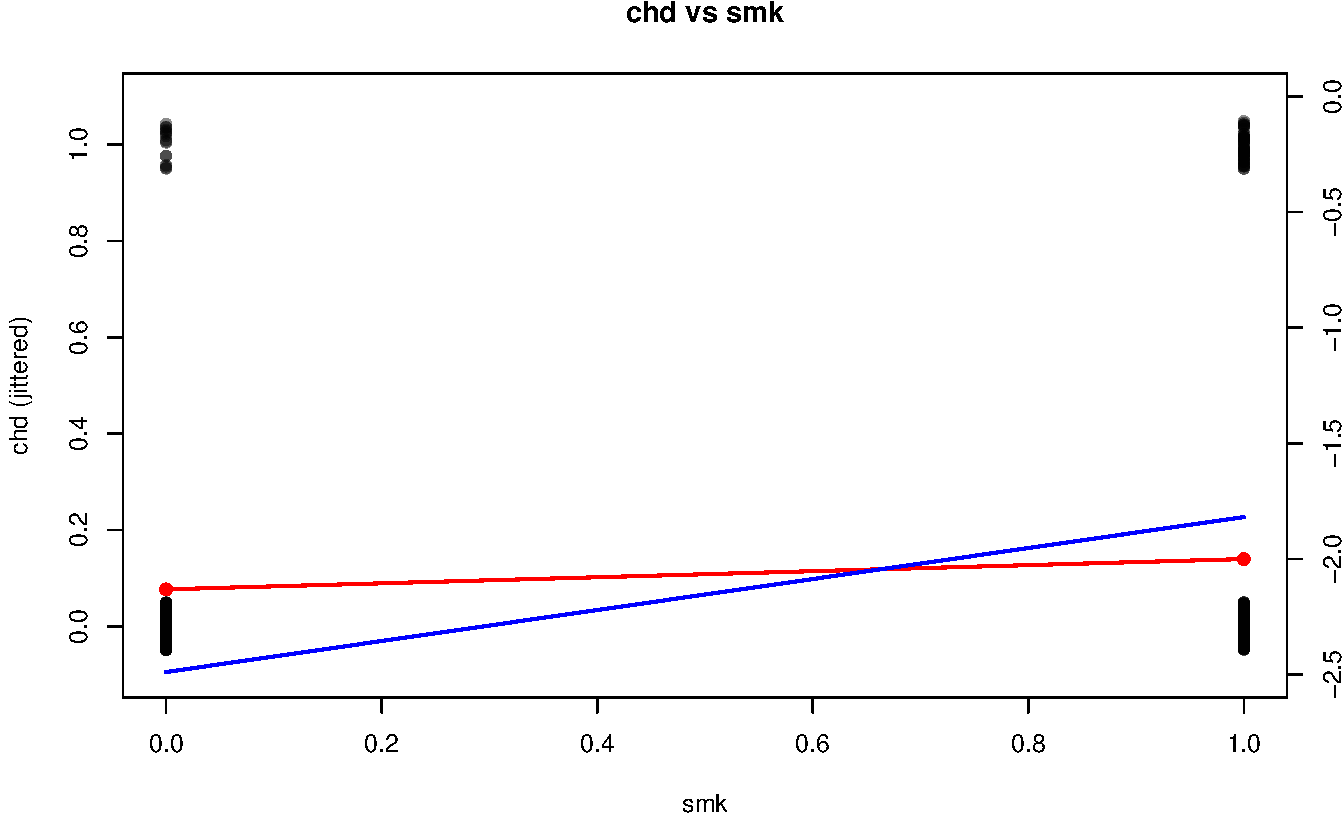
\includegraphics[keepaspectratio]{unit4-lr/logistic_files/figure-pdf/chd-univariate-2x2-jitter-fixedlogit-1.pdf}}

\begin{verbatim}

Call:
glm(formula = reformulate(v, response = "chd"), family = binomial(), 
    data = CHD.data)

Coefficients:
             Estimate Std. Error z value Pr(>|z|)    
(Intercept) -3.837912   0.629805  -6.094  1.1e-09 ***
sbp          0.012154   0.004036   3.011   0.0026 ** 
---
Signif. codes:  0 '***' 0.001 '**' 0.01 '*' 0.05 '.' 0.1 ' ' 1

(Dispersion parameter for binomial family taken to be 1)

    Null deviance: 438.56  on 608  degrees of freedom
Residual deviance: 430.06  on 607  degrees of freedom
AIC: 434.06

Number of Fisher Scoring iterations: 4
\end{verbatim}

\pandocbounded{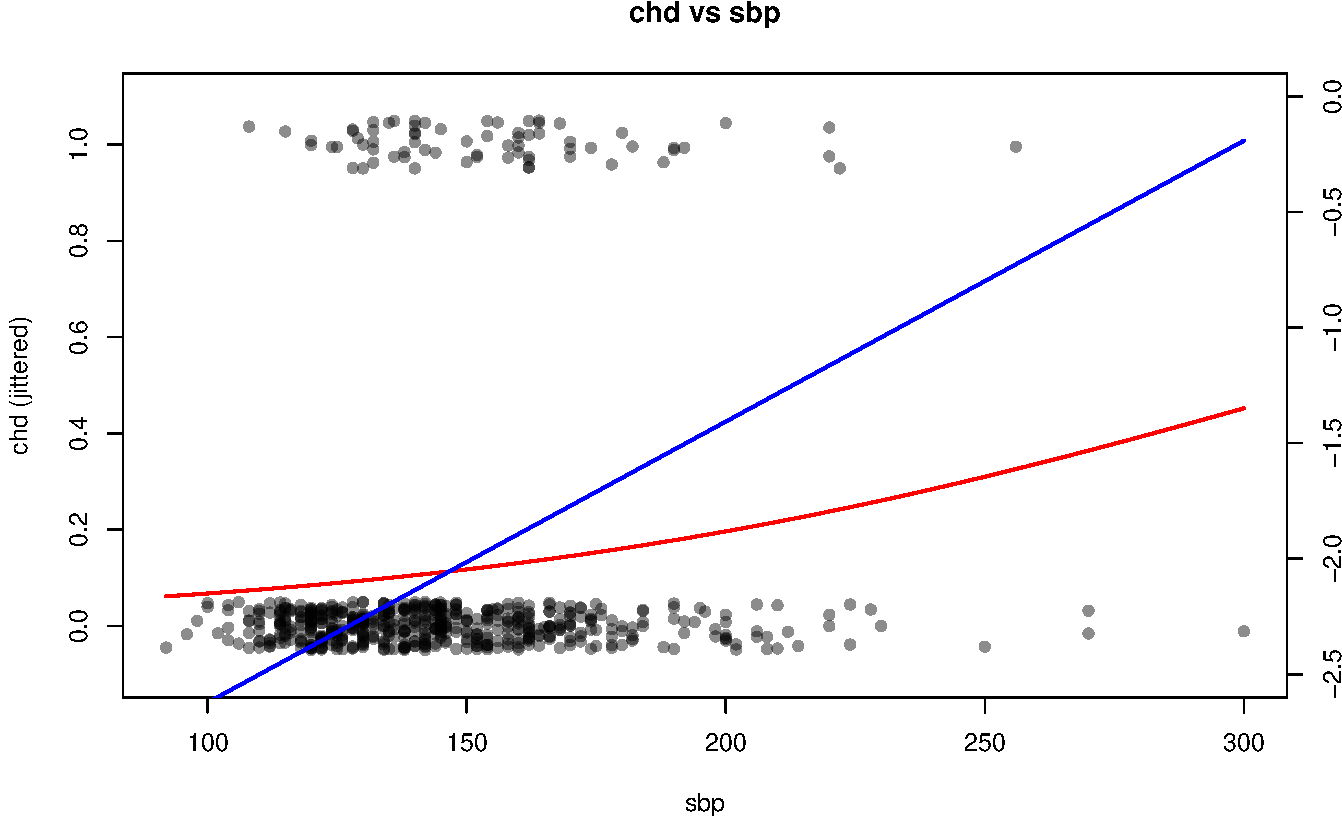
\includegraphics[keepaspectratio]{unit4-lr/logistic_files/figure-pdf/chd-univariate-2x2-jitter-fixedlogit-2.pdf}}

\begin{verbatim}

Call:
glm(formula = reformulate(v, response = "chd"), family = binomial(), 
    data = CHD.data)

Coefficients:
            Estimate Std. Error z value Pr(>|z|)    
(Intercept) -4.47833    0.75610  -5.923 3.16e-09 ***
age          0.04445    0.01315   3.381 0.000723 ***
---
Signif. codes:  0 '***' 0.001 '**' 0.01 '*' 0.05 '.' 0.1 ' ' 1

(Dispersion parameter for binomial family taken to be 1)

    Null deviance: 438.56  on 608  degrees of freedom
Residual deviance: 427.22  on 607  degrees of freedom
AIC: 431.22

Number of Fisher Scoring iterations: 5
\end{verbatim}

\pandocbounded{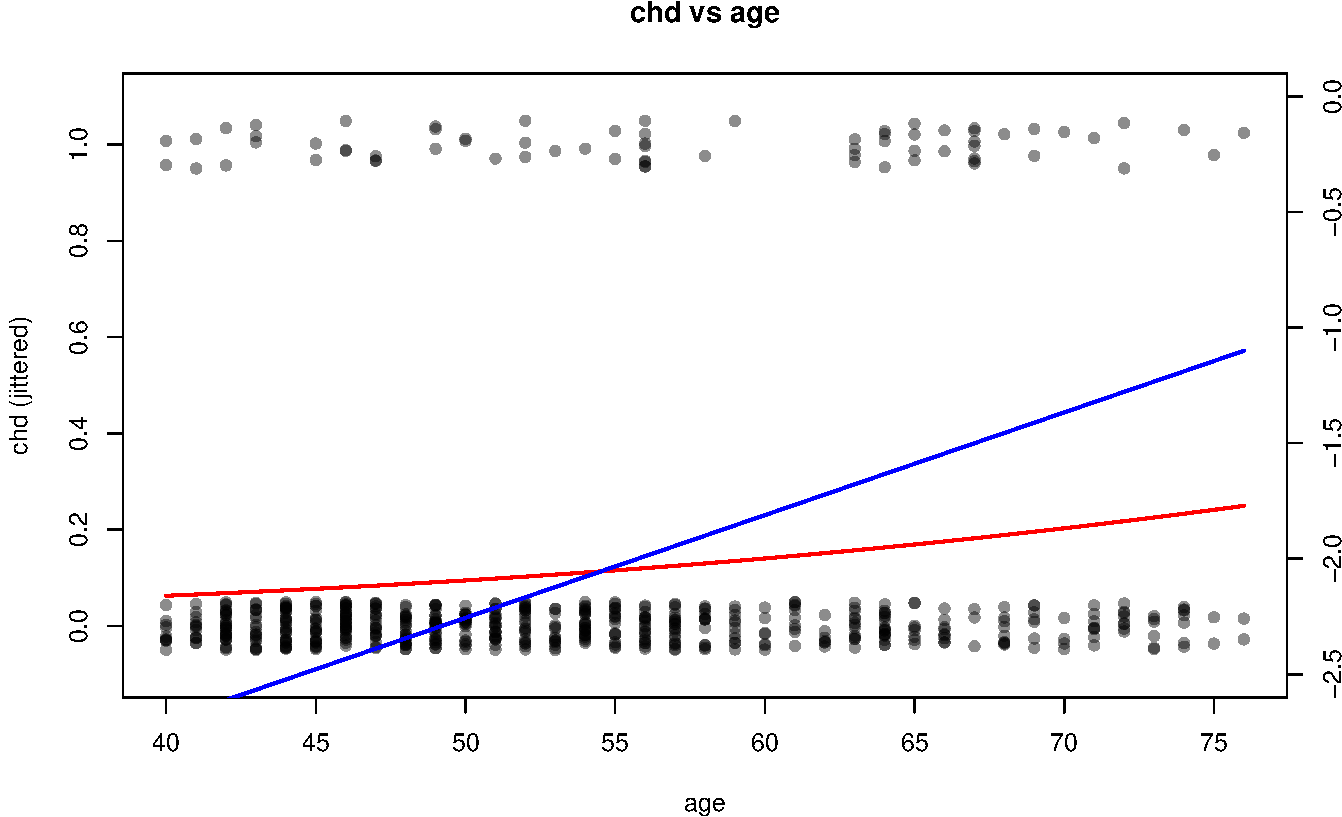
\includegraphics[keepaspectratio]{unit4-lr/logistic_files/figure-pdf/chd-univariate-2x2-jitter-fixedlogit-3.pdf}}

\begin{verbatim}

Call:
glm(formula = reformulate(v, response = "chd"), family = binomial(), 
    data = CHD.data)

Coefficients:
             Estimate Std. Error z value Pr(>|z|)    
(Intercept) -3.538260   0.686879  -5.151 2.59e-07 ***
chl          0.007004   0.003064   2.286   0.0223 *  
---
Signif. codes:  0 '***' 0.001 '**' 0.01 '*' 0.05 '.' 0.1 ' ' 1

(Dispersion parameter for binomial family taken to be 1)

    Null deviance: 438.56  on 608  degrees of freedom
Residual deviance: 433.42  on 607  degrees of freedom
AIC: 437.42

Number of Fisher Scoring iterations: 4
\end{verbatim}

\pandocbounded{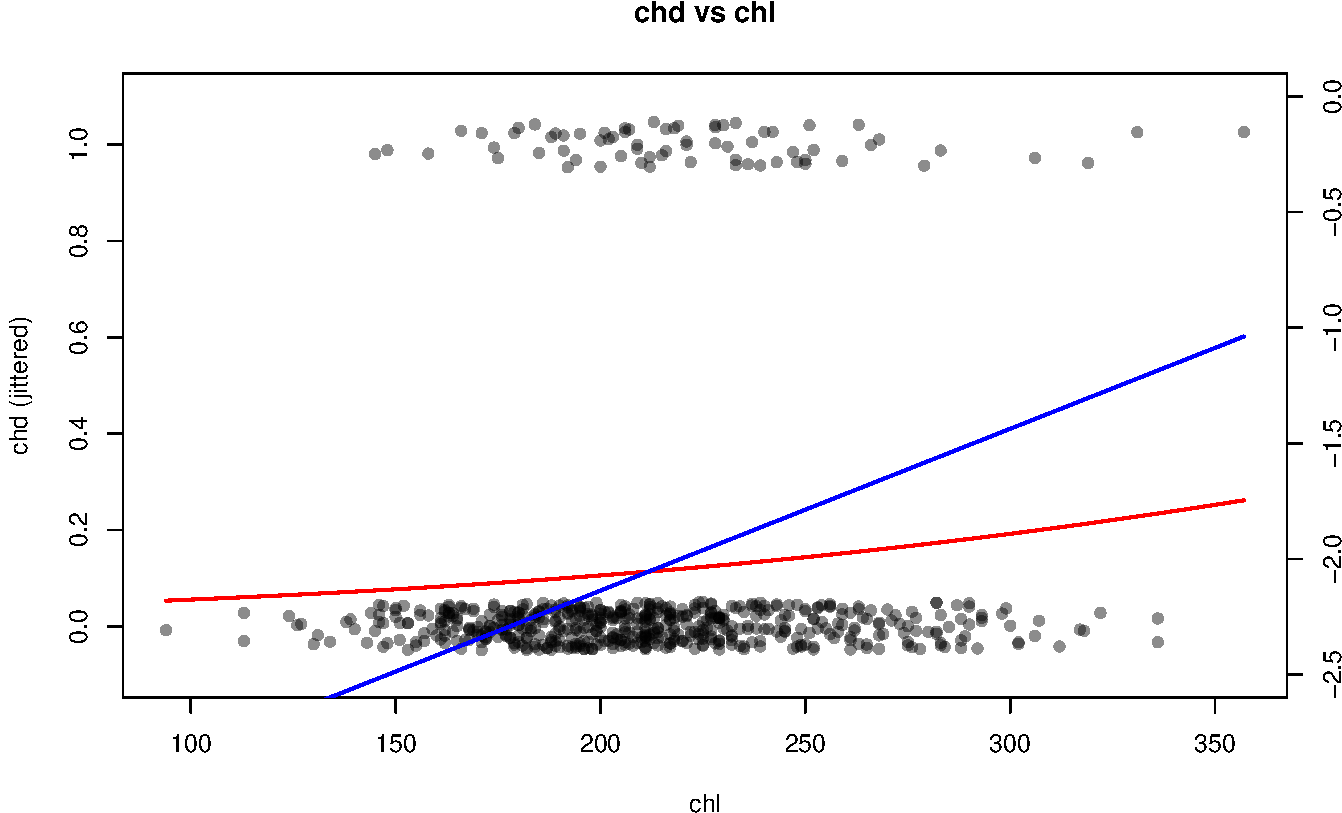
\includegraphics[keepaspectratio]{unit4-lr/logistic_files/figure-pdf/chd-univariate-2x2-jitter-fixedlogit-4.pdf}}

\subsection{Fit Logistic Regression Model with all
variables}\label{fit-logistic-regression-model-with-all-variables}

We fit a logistic regression with a logit link:

\begin{Shaded}
\begin{Highlighting}[]
\NormalTok{fit1\_chd }\OtherTok{\textless{}{-}} \FunctionTok{glm}\NormalTok{(}
\NormalTok{  chd }\SpecialCharTok{\textasciitilde{}}\NormalTok{ smk }\SpecialCharTok{+}\NormalTok{ cat }\SpecialCharTok{+}\NormalTok{ sbp }\SpecialCharTok{+}\NormalTok{ age }\SpecialCharTok{+}\NormalTok{ chl }\SpecialCharTok{+}\NormalTok{ ecg }\SpecialCharTok{+}\NormalTok{ hpt,}
  \AttributeTok{data =}\NormalTok{ CHD.data,}
  \AttributeTok{family =} \FunctionTok{binomial}\NormalTok{(}\AttributeTok{link =} \StringTok{"logit"}\NormalTok{)}
\NormalTok{)}
\FunctionTok{summary}\NormalTok{(fit1\_chd)}
\end{Highlighting}
\end{Shaded}

\begin{verbatim}

Call:
glm(formula = chd ~ smk + cat + sbp + age + chl + ecg + hpt, 
    family = binomial(link = "logit"), data = CHD.data)

Coefficients:
             Estimate Std. Error z value Pr(>|z|)    
(Intercept) -6.048892   1.345165  -4.497  6.9e-06 ***
smk          0.855951   0.306505   2.793  0.00523 ** 
cat          0.732763   0.376129   1.948  0.05139 .  
sbp         -0.006995   0.006976  -1.003  0.31600    
age          0.033956   0.015344   2.213  0.02690 *  
chl          0.008970   0.003274   2.740  0.00615 ** 
ecg          0.417776   0.295553   1.414  0.15750    
hpt          0.655498   0.359976   1.821  0.06861 .  
---
Signif. codes:  0 '***' 0.001 '**' 0.01 '*' 0.05 '.' 0.1 ' ' 1

(Dispersion parameter for binomial family taken to be 1)

    Null deviance: 438.56  on 608  degrees of freedom
Residual deviance: 399.35  on 601  degrees of freedom
AIC: 415.35

Number of Fisher Scoring iterations: 5
\end{verbatim}

\textbf{Notes for interpretation:}

\begin{itemize}
\tightlist
\item
  Positive coefficients increase the log-odds of CHD; negative
  coefficients decrease it.
\item
  For indicator variables (e.g., \texttt{smk}), \texttt{exp(beta)} is
  the adjusted odds ratio comparing the group with value 1 versus 0,
  holding others fixed.
\item
  For continuous predictors (e.g., \texttt{sbp}, \texttt{age}),
  \texttt{exp(beta)} is the multiplicative change in the odds for a
  one‑unit increase. For a \emph{d}-unit increase, the OR is
  \texttt{exp(d\ *\ beta)}.
\end{itemize}

\section{Inference for Coefficients: Confidence Intervals and Covariance
Matrix}\label{inference-for-coefficients-confidence-intervals-and-covariance-matrix}

We extract profile‑likelihood CIs and the covariance matrix to confirm
standard errors.

\begin{Shaded}
\begin{Highlighting}[]
\NormalTok{ci\_95 }\OtherTok{\textless{}{-}} \FunctionTok{confint}\NormalTok{(fit1\_chd, }\AttributeTok{level =} \FloatTok{0.95}\NormalTok{)     }\CommentTok{\# profile{-}likelihood CI}
\NormalTok{vcov\_mat }\OtherTok{\textless{}{-}} \FunctionTok{vcov}\NormalTok{(fit1\_chd)                    }\CommentTok{\# covariance matrix of coefficients}
\NormalTok{se\_vec   }\OtherTok{\textless{}{-}} \FunctionTok{sqrt}\NormalTok{(}\FunctionTok{diag}\NormalTok{(vcov\_mat))          }\CommentTok{\# standard errors}

\NormalTok{ci\_95}
\end{Highlighting}
\end{Shaded}

\begin{verbatim}
                   2.5 %       97.5 %
(Intercept) -8.718003347 -3.427904298
smk          0.275699158  1.483333169
cat         -0.006873216  1.471885644
sbp         -0.021166144  0.006266328
age          0.003687290  0.064005215
chl          0.002533226  0.015404292
ecg         -0.171584621  0.990632546
hpt         -0.050184520  1.364993401
\end{verbatim}

\begin{Shaded}
\begin{Highlighting}[]
\NormalTok{vcov\_mat}
\end{Highlighting}
\end{Shaded}

\begin{verbatim}
             (Intercept)           smk           cat           sbp
(Intercept)  1.809468553 -1.014526e-01  0.1391440386 -4.908229e-03
smk         -0.101452600  9.394560e-02 -0.0032961000 -1.653230e-04
cat          0.139144039 -3.296100e-03  0.1414730484 -9.299960e-04
sbp         -0.004908229 -1.653230e-04 -0.0009299960  4.866901e-05
age         -0.011142995  7.738971e-04 -0.0017879998 -1.311191e-05
chl         -0.002111134  3.161443e-05  0.0003146354 -1.821907e-06
ecg          0.003442546  9.255483e-03 -0.0204455233 -2.982539e-04
hpt          0.139817180  6.954592e-03 -0.0044220690 -1.486400e-03
                      age           chl           ecg           hpt
(Intercept) -1.114300e-02 -2.111134e-03  3.442546e-03  1.398172e-01
smk          7.738971e-04  3.161443e-05  9.255483e-03  6.954592e-03
cat         -1.788000e-03  3.146354e-04 -2.044552e-02 -4.422069e-03
sbp         -1.311191e-05 -1.821907e-06 -2.982539e-04 -1.486400e-03
age          2.354442e-04 -1.480501e-06 -4.972374e-05  4.044434e-04
chl         -1.480501e-06  1.071766e-05  5.040548e-05 -6.046197e-05
ecg         -4.972374e-05  5.040548e-05  8.735130e-02  9.506863e-04
hpt          4.044434e-04 -6.046197e-05  9.506863e-04  1.295828e-01
\end{verbatim}

\begin{Shaded}
\begin{Highlighting}[]
\NormalTok{se\_vec  }\CommentTok{\# should match the SE column in summary(fit1\_chd)}
\end{Highlighting}
\end{Shaded}

\begin{verbatim}
(Intercept)         smk         cat         sbp         age         chl 
1.345164879 0.306505459 0.376129032 0.006976318 0.015344190 0.003273784 
        ecg         hpt 
0.295552531 0.359976081 
\end{verbatim}

\section{Inference for Odds Ratios}\label{inference-for-odds-ratios}

\subsection{Interpretation of Odds Ratios in Logistic
Regression}\label{interpretation-of-odds-ratios-in-logistic-regression}

A multiple logistic regression model expresses the log-odds (logit) of
an event as a linear function of predictors:

\[
\log\left(\frac{p}{1-p}\right)
= \beta_0 + \beta_1 x_1 + \beta_2 x_2 + \cdots + \beta_k x_k.
\]

Here,

\begin{itemize}
\tightlist
\item
  \(p = \Pr(Y = 1 \mid x_1, x_2, \ldots, x_k)\) is the probability of
  the event,
\item
  \(\beta_0\) is the intercept, and
\item
  each \(\beta_j\) represents the \textbf{change in the log-odds} of the
  event per one-unit increase in \(x_j\), \emph{holding all other
  variables constant}.
\end{itemize}

Exponentiating both sides gives the model in odds form:

\[
\frac{p}{1-p}
= \exp(\beta_0)
\times \exp(\beta_1 x_1)
\times \exp(\beta_2 x_2)
\times \cdots
\times \exp(\beta_k x_k).
\]

\textbf{An R function for OR at two Profiles}

The or\_from\_predict R function is a utility designed to calculate the
Odds Ratio (OR) and its 95\% confidence interval (CI) between two
specific covariate profiles (new1 and new0) for a given logistic
regression model (fit). The calculation is performed on the link (logit)
scale. For a logistic model
\(\text{logit}(p) = \eta = \mathbf{X}\boldsymbol{\beta}\), the log-Odds
Ratio (logOR) is the difference between the linear predictors
(\(\eta_1, \eta_0\)) for the two profiles:
\begin{equation}\phantomsection\label{eq-logor}{\widehat{\text{logOR}} = \eta_1 - \eta_0 = (\mathbf{x}_1^T - \mathbf{x}_0^T) \boldsymbol{\beta} = \mathbf{c}^T \boldsymbol{\beta}}\end{equation}

Here, \(\mathbf{c} = \mathbf{x}_1 - \mathbf{x}_0\) is the linear
contrast vector derived from the model matrices of the two profiles. The
function estimates the variance of this contrast as
\(\text{Var}(\widehat{\text{logOR}}) = \mathbf{c}^T \mathbf{V} \mathbf{c}\),
where \(\mathbf{V}\) is the model's variance-covariance matrix
(vcov(fit)). The standard error
\(SE = \sqrt{\mathbf{c}^T \mathbf{V} \mathbf{c}}\) is used to compute
the \(100(1-\alpha)\%\) confidence interval for the logOR:
\[\widehat{\text{logOR}} \pm z_{1-\alpha/2} \times SE.\] These values
(estimate and CI bounds) are then exponentiated to produce the final
\(\widehat{\text{OR}} = \exp(\widehat{\text{logOR}})\) and its 95\% CI.
The function also prints two helpful summaries to the console: a data
frame showing only the variables that differ between the new0 and new1
profiles, and a 2x3 table presenting the estimates and CIs for both the
OR and the logOR.

\textbf{The R function to find ORs}

\begin{Shaded}
\begin{Highlighting}[]
\CommentTok{\# Compute OR and 95\% CI via predict() on the LINK scale}
\CommentTok{\# OR = exp( eta(new1) {-} eta(new0) ), where eta(.) = logit\{π(.)\}}
\CommentTok{\# Compute OR via predict() contrast on the LINK scale, also:}
\CommentTok{\# (ii) print a 2{-}row data.frame of only variables that differ between new0 and new1}
\CommentTok{\# (iii) print a 2x3 table (rows: OR, logOR; cols: Estimate, CI\_low, CI\_up)}
\NormalTok{or\_from\_predict }\OtherTok{\textless{}{-}} \ControlFlowTok{function}\NormalTok{(fit, new1, new0, }\AttributeTok{level =} \FloatTok{0.95}\NormalTok{, }\AttributeTok{digits =} \DecValTok{4}\NormalTok{, }\AttributeTok{tol =} \FloatTok{1e{-}12}\NormalTok{) \{}
  \FunctionTok{stopifnot}\NormalTok{(}\FunctionTok{is.data.frame}\NormalTok{(new1), }\FunctionTok{is.data.frame}\NormalTok{(new0))}

  \CommentTok{\# {-}{-}{-} REFACTORED SECTION START {-}{-}{-}}
  \CommentTok{\# {-}{-}{-}{-} (ii) Two{-}row data.frame with only changed variables {-}{-}{-}{-}}
  
  \CommentTok{\# Helper function to find differing variables between two profiles}
  \CommentTok{\# This is defined *inside* or\_from\_predict for encapsulation}
\NormalTok{  get\_changed\_vars }\OtherTok{\textless{}{-}} \ControlFlowTok{function}\NormalTok{(d0, d1, tolerance) \{}
\NormalTok{    common }\OtherTok{\textless{}{-}} \FunctionTok{intersect}\NormalTok{(}\FunctionTok{names}\NormalTok{(d0), }\FunctionTok{names}\NormalTok{(d1))}
\NormalTok{    diffv  }\OtherTok{\textless{}{-}} \FunctionTok{vapply}\NormalTok{(common, }\ControlFlowTok{function}\NormalTok{(nm) \{}
\NormalTok{      x0 }\OtherTok{\textless{}{-}}\NormalTok{ d0[[nm]]; x1 }\OtherTok{\textless{}{-}}\NormalTok{ d1[[nm]]}
      \ControlFlowTok{if}\NormalTok{ (}\FunctionTok{is.numeric}\NormalTok{(x0) }\SpecialCharTok{\&\&} \FunctionTok{is.numeric}\NormalTok{(x1)) \{}
        \SpecialCharTok{!}\FunctionTok{isTRUE}\NormalTok{(}\FunctionTok{all.equal}\NormalTok{(}\FunctionTok{as.numeric}\NormalTok{(x0), }\FunctionTok{as.numeric}\NormalTok{(x1), }\AttributeTok{tolerance =}\NormalTok{ tolerance))}
\NormalTok{      \} }\ControlFlowTok{else}\NormalTok{ \{}
        \SpecialCharTok{!}\FunctionTok{identical}\NormalTok{(x0, x1)}
\NormalTok{      \}}
\NormalTok{    \}, }\FunctionTok{logical}\NormalTok{(}\DecValTok{1}\NormalTok{))}
    
\NormalTok{    keep }\OtherTok{\textless{}{-}}\NormalTok{ common[diffv]}
    \ControlFlowTok{if}\NormalTok{ (}\FunctionTok{length}\NormalTok{(keep) }\SpecialCharTok{==} \DecValTok{0}\NormalTok{L) \{}
\NormalTok{      out }\OtherTok{\textless{}{-}} \FunctionTok{data.frame}\NormalTok{(}\StringTok{\textasciigrave{}}\AttributeTok{\_no\_changes\_}\StringTok{\textasciigrave{}} \OtherTok{=} \StringTok{"no differences"}\NormalTok{)}
      \FunctionTok{rownames}\NormalTok{(out) }\OtherTok{\textless{}{-}} \FunctionTok{c}\NormalTok{(}\StringTok{"new0"}\NormalTok{, }\StringTok{"new1"}\NormalTok{)}
      \FunctionTok{return}\NormalTok{(out)}
\NormalTok{    \}}
\NormalTok{    out }\OtherTok{\textless{}{-}} \FunctionTok{rbind}\NormalTok{(d0[keep], d1[keep])}
    \FunctionTok{rownames}\NormalTok{(out) }\OtherTok{\textless{}{-}} \FunctionTok{c}\NormalTok{(}\StringTok{"new0"}\NormalTok{, }\StringTok{"new1"}\NormalTok{)}
\NormalTok{    out}
\NormalTok{  \}}
  
  \CommentTok{\# Call the helper function}
\NormalTok{  changes\_df }\OtherTok{\textless{}{-}} \FunctionTok{get\_changed\_vars}\NormalTok{(new0, new1, tol)}
  \CommentTok{\# {-}{-}{-} REFACTORED SECTION }\RegionMarkerTok{END}\CommentTok{ {-}{-}{-}}


  \CommentTok{\# {-}{-}{-}{-} Linear contrast for log{-}OR and its variance {-}{-}{-}{-}}
  
  \CommentTok{\# (i) Calculate logOR estimate using predict(type="link")}
  \CommentTok{\# eta(.) = logit\{p(.)\}}
\NormalTok{  eta1 }\OtherTok{\textless{}{-}} \FunctionTok{predict}\NormalTok{(fit, }\AttributeTok{newdata =}\NormalTok{ new1, }\AttributeTok{type =} \StringTok{"link"}\NormalTok{)}
\NormalTok{  eta0 }\OtherTok{\textless{}{-}} \FunctionTok{predict}\NormalTok{(fit, }\AttributeTok{newdata =}\NormalTok{ new0, }\AttributeTok{type =} \StringTok{"link"}\NormalTok{)}
\NormalTok{  logOR\_hat }\OtherTok{\textless{}{-}} \FunctionTok{as.numeric}\NormalTok{(eta1 }\SpecialCharTok{{-}}\NormalTok{ eta0) }\CommentTok{\# logOR = eta1 {-} eta0}
  
  \CommentTok{\# (ii) Calculate standard error using the contrast vector \textquotesingle{}cvec\textquotesingle{}}
\NormalTok{  X1 }\OtherTok{\textless{}{-}} \FunctionTok{model.matrix}\NormalTok{(}\FunctionTok{delete.response}\NormalTok{(}\FunctionTok{terms}\NormalTok{(fit)), }\AttributeTok{data =}\NormalTok{ new1)}
\NormalTok{  X0 }\OtherTok{\textless{}{-}} \FunctionTok{model.matrix}\NormalTok{(}\FunctionTok{delete.response}\NormalTok{(}\FunctionTok{terms}\NormalTok{(fit)), }\AttributeTok{data =}\NormalTok{ new0)}
\NormalTok{  cvec      }\OtherTok{\textless{}{-}} \FunctionTok{as.numeric}\NormalTok{(X1 }\SpecialCharTok{{-}}\NormalTok{ X0)}
\NormalTok{  V         }\OtherTok{\textless{}{-}} \FunctionTok{vcov}\NormalTok{(fit)}
\NormalTok{  se\_logOR  }\OtherTok{\textless{}{-}} \FunctionTok{sqrt}\NormalTok{(}\FunctionTok{as.numeric}\NormalTok{(}\FunctionTok{t}\NormalTok{(cvec) }\SpecialCharTok{\%*\%}\NormalTok{ V }\SpecialCharTok{\%*\%}\NormalTok{ cvec))}

\NormalTok{  alpha  }\OtherTok{\textless{}{-}} \DecValTok{1} \SpecialCharTok{{-}}\NormalTok{ level}
\NormalTok{  z      }\OtherTok{\textless{}{-}} \FunctionTok{qnorm}\NormalTok{(}\DecValTok{1} \SpecialCharTok{{-}}\NormalTok{ alpha }\SpecialCharTok{/} \DecValTok{2}\NormalTok{)}
\NormalTok{  ci\_log }\OtherTok{\textless{}{-}} \FunctionTok{c}\NormalTok{(logOR\_hat }\SpecialCharTok{{-}}\NormalTok{ z }\SpecialCharTok{*}\NormalTok{ se\_logOR, logOR\_hat }\SpecialCharTok{+}\NormalTok{ z }\SpecialCharTok{*}\NormalTok{ se\_logOR)}

  \CommentTok{\# {-}{-}{-}{-} 2x3 table: rows OR and logOR; columns Estimate, CI\_low, CI\_up {-}{-}{-}{-}}
\NormalTok{  res\_tab }\OtherTok{\textless{}{-}} \FunctionTok{data.frame}\NormalTok{(}
    \AttributeTok{Estimate =} \FunctionTok{c}\NormalTok{(}\FunctionTok{exp}\NormalTok{(logOR\_hat),          logOR\_hat),}
    \AttributeTok{CI\_low   =} \FunctionTok{c}\NormalTok{(}\FunctionTok{exp}\NormalTok{(ci\_log[}\DecValTok{1}\NormalTok{L]),         ci\_log[}\DecValTok{1}\NormalTok{L]),}
    \AttributeTok{CI\_up    =} \FunctionTok{c}\NormalTok{(}\FunctionTok{exp}\NormalTok{(ci\_log[}\DecValTok{2}\NormalTok{L]),         ci\_log[}\DecValTok{2}\NormalTok{L]),}
    \AttributeTok{row.names =} \FunctionTok{c}\NormalTok{(}\StringTok{"OR"}\NormalTok{, }\StringTok{"logOR"}\NormalTok{)}
\NormalTok{  )}

  \CommentTok{\# {-}{-}{-}{-} Print requested items {-}{-}{-}{-}}
  \FunctionTok{cat}\NormalTok{(}\StringTok{"}\SpecialCharTok{\textbackslash{}n}\StringTok{Variables that differ between new0 and new1:}\SpecialCharTok{\textbackslash{}n}\StringTok{"}\NormalTok{)}
  \FunctionTok{print}\NormalTok{(changes\_df)}
  \FunctionTok{cat}\NormalTok{(}\StringTok{"}\SpecialCharTok{\textbackslash{}n}\StringTok{Odds Ratio summary:}\SpecialCharTok{\textbackslash{}n}\StringTok{"}\NormalTok{)}
  \FunctionTok{print}\NormalTok{(}\FunctionTok{round}\NormalTok{(res\_tab, }\AttributeTok{digits =}\NormalTok{ digits)) }\CommentTok{\# Added rounding for neatness}

  \CommentTok{\# {-}{-}{-}{-} Return (invisibly) {-}{-}{-}{-}}
  \FunctionTok{invisible}\NormalTok{(}\FunctionTok{list}\NormalTok{(}
    \AttributeTok{OR        =} \FunctionTok{exp}\NormalTok{(logOR\_hat),}
    \AttributeTok{CI\_OR     =} \FunctionTok{exp}\NormalTok{(ci\_log),}
    \AttributeTok{logOR     =}\NormalTok{ logOR\_hat,}
    \AttributeTok{CI\_logOR  =}\NormalTok{ ci\_log,}
    \AttributeTok{se\_logOR  =}\NormalTok{ se\_logOR,}
    \AttributeTok{changes   =}\NormalTok{ changes\_df,}
    \AttributeTok{table     =}\NormalTok{ res\_tab}
\NormalTok{  ))}
\NormalTok{\}}

\CommentTok{\# {-}{-}{-} Example usage {-}{-}{-}}
\CommentTok{\# Suppose \textquotesingle{}fit1\_chd\textquotesingle{} is your fitted model and \textquotesingle{}CHD.data\textquotesingle{} is your data}
\CommentTok{\# base\_prof \textless{}{-} as.data.frame(lapply(CHD.data, function(col) if (is.numeric(col)) mean(col) else col[1]))}
\CommentTok{\# new0 \textless{}{-} base\_prof; new0$smk \textless{}{-} 0}
\CommentTok{\# new1 \textless{}{-} base\_prof; new1$smk \textless{}{-} 1}
\CommentTok{\# or\_from\_predict(fit1\_chd, new1 = new1, new0 = new0)}


\NormalTok{mean\_profile }\OtherTok{\textless{}{-}} \ControlFlowTok{function}\NormalTok{(data, }\AttributeTok{vars\_binary\_as =} \FunctionTok{c}\NormalTok{(}\DecValTok{0}\NormalTok{,}\DecValTok{1}\NormalTok{)) \{}
  \CommentTok{\# Build a single{-}row data.frame of typical values:}
\NormalTok{  out }\OtherTok{\textless{}{-}} \FunctionTok{lapply}\NormalTok{(data, }\ControlFlowTok{function}\NormalTok{(col) \{}
    \ControlFlowTok{if}\NormalTok{ (}\FunctionTok{is.numeric}\NormalTok{(col)) \{}
      \CommentTok{\# If strictly 0/1, keep mean (works fine for GLM prediction),}
      \CommentTok{\# or switch to mode if you prefer.}
      \ControlFlowTok{if}\NormalTok{ (}\FunctionTok{all}\NormalTok{(col }\SpecialCharTok{\%in\%} \FunctionTok{c}\NormalTok{(}\DecValTok{0}\NormalTok{,}\DecValTok{1}\NormalTok{))) }\FunctionTok{mean}\NormalTok{(col) }\ControlFlowTok{else} \FunctionTok{mean}\NormalTok{(col, }\AttributeTok{na.rm =} \ConstantTok{TRUE}\NormalTok{)}
\NormalTok{    \} }\ControlFlowTok{else}\NormalTok{ \{}
      \CommentTok{\# Fallback to first level for factors/characters}
      \ControlFlowTok{if}\NormalTok{ (}\FunctionTok{is.factor}\NormalTok{(col)) }\FunctionTok{levels}\NormalTok{(col)[}\DecValTok{1}\NormalTok{] }\ControlFlowTok{else} \FunctionTok{unique}\NormalTok{(col)[}\DecValTok{1}\NormalTok{]}
\NormalTok{    \}}
\NormalTok{  \})}
  \FunctionTok{as.data.frame}\NormalTok{(out)}
\NormalTok{\}}
\end{Highlighting}
\end{Shaded}

\subsection{Examples of Finding ORs and Their CIs for the CHD
Dataset}\label{examples-of-finding-ors-and-their-cis-for-the-chd-dataset}

\subsubsection{\texorpdfstring{OR Smoking (\texttt{smk}) (1 vs
0)}{OR Smoking (smk) (1 vs 0)}}\label{or-smoking-smk-1-vs-0}

\begin{Shaded}
\begin{Highlighting}[]
\DocumentationTok{\#\# 1) Smoking OR: smk = 1 vs 0 (other vars at their means)}
\CommentTok{\# Example profiles at sample means (adjust as you like)}
\NormalTok{base\_prof }\OtherTok{\textless{}{-}} \FunctionTok{mean\_profile}\NormalTok{(CHD.data)}
\NormalTok{new0 }\OtherTok{\textless{}{-}}\NormalTok{ base\_prof; new0}\SpecialCharTok{$}\NormalTok{smk }\OtherTok{\textless{}{-}} \DecValTok{0}
\NormalTok{new1 }\OtherTok{\textless{}{-}}\NormalTok{ base\_prof; new1}\SpecialCharTok{$}\NormalTok{smk }\OtherTok{\textless{}{-}} \DecValTok{1}

\NormalTok{res\_smk }\OtherTok{\textless{}{-}} \FunctionTok{or\_from\_predict}\NormalTok{(fit1\_chd, }\AttributeTok{new1 =}\NormalTok{ new1, }\AttributeTok{new0 =}\NormalTok{ new0)}
\end{Highlighting}
\end{Shaded}

\begin{verbatim}

Variables that differ between new0 and new1:
     smk
new0   0
new1   1

Odds Ratio summary:
      Estimate CI_low  CI_up
OR      2.3536 1.2907 4.2917
logOR   0.8560 0.2552 1.4567
\end{verbatim}

\textbf{How to read this:}

\begin{itemize}
\tightlist
\item
  \texttt{OR\_smk\ \textgreater{}\ 1} suggests higher odds of CHD among
  smokers (adjusted for other variables). If the 95\% CI excludes 1, the
  association is statistically significant at the 5\% level.
\end{itemize}

\subsubsection{\texorpdfstring{OR for Systolic Blood Pressure
(\texttt{sbp}): from 120 to
160}{OR for Systolic Blood Pressure (sbp): from 120 to 160}}\label{or-for-systolic-blood-pressure-sbp-from-120-to-160}

We compute the adjusted OR for a 40‑unit increase in \texttt{sbp} (from
120 to 160):

\begin{Shaded}
\begin{Highlighting}[]
\DocumentationTok{\#\# 2) SBP OR: 160 vs 120 (other vars at their means)}
\NormalTok{new0 }\OtherTok{\textless{}{-}}\NormalTok{ base\_prof; new0}\SpecialCharTok{$}\NormalTok{sbp }\OtherTok{\textless{}{-}} \DecValTok{120}
\NormalTok{new1 }\OtherTok{\textless{}{-}}\NormalTok{ base\_prof; new1}\SpecialCharTok{$}\NormalTok{sbp }\OtherTok{\textless{}{-}} \DecValTok{160}

\NormalTok{res\_sbp }\OtherTok{\textless{}{-}} \FunctionTok{or\_from\_predict}\NormalTok{(fit1\_chd, }\AttributeTok{new1 =}\NormalTok{ new1, }\AttributeTok{new0 =}\NormalTok{ new0)}
\end{Highlighting}
\end{Shaded}

\begin{verbatim}

Variables that differ between new0 and new1:
     sbp
new0 120
new1 160

Odds Ratio summary:
      Estimate  CI_low  CI_up
OR      0.7559  0.4375 1.3062
logOR  -0.2798 -0.8267 0.2671
\end{verbatim}

\subsubsection{OR for Combined Effects of Two Variables: Smoking with an
Age
Difference}\label{or-for-combined-effects-of-two-variables-smoking-with-an-age-difference}

Suppose we compare two groups that differ in \textbf{smoking status} and
\textbf{age}:

\begin{itemize}
\tightlist
\item
  \textbf{Group A:} \texttt{smk\ =\ 1}, \texttt{age\ =\ 50} (all other
  covariates equal)
\item
  \textbf{Group B:} \texttt{smk\ =\ 0}, \texttt{age\ =\ 30}
\end{itemize}

The log‑odds contrast is (\(A = \beta_{smk} + (50-20)\beta_{age}\)), so
the OR is (\(\exp(A)\)).

\begin{Shaded}
\begin{Highlighting}[]
\NormalTok{new0 }\OtherTok{\textless{}{-}}\NormalTok{ base\_prof; new0}\SpecialCharTok{$}\NormalTok{age }\OtherTok{\textless{}{-}} \DecValTok{30}\NormalTok{; new0}\SpecialCharTok{$}\NormalTok{smk }\OtherTok{\textless{}{-}} \DecValTok{0}
\NormalTok{new1 }\OtherTok{\textless{}{-}}\NormalTok{ base\_prof; new1}\SpecialCharTok{$}\NormalTok{age }\OtherTok{\textless{}{-}} \DecValTok{50}\NormalTok{; new1}\SpecialCharTok{$}\NormalTok{smk }\OtherTok{\textless{}{-}} \DecValTok{1}

\NormalTok{res\_ageAsmk }\OtherTok{\textless{}{-}} \FunctionTok{or\_from\_predict}\NormalTok{(fit1\_chd, }\AttributeTok{new1 =}\NormalTok{ new1, }\AttributeTok{new0 =}\NormalTok{ new0)}
\end{Highlighting}
\end{Shaded}

\begin{verbatim}

Variables that differ between new0 and new1:
     age smk
new0  30   0
new1  50   1

Odds Ratio summary:
      Estimate CI_low   CI_up
OR      4.6417 1.8546 11.6168
logOR   1.5351 0.6177  2.4525
\end{verbatim}

\section{Assessing Statistical Significance with Wilks' Theorem
(Analogue of F-test for
OLS)}\label{assessing-statistical-significance-with-wilks-theorem-analogue-of-f-test-for-ols}

In the context of logistic regression, Wilks' theorem provides the basis
for the Likelihood Ratio Test (LRT) used to assess the significance of
predictor variables. The theorem states that when comparing a full model
(\(M_1\)) to a nested null model (\(M_0\)), the test statistic,
\(\Lambda\), asymptotically follows a chi-squared (\(\chi^2\))
distribution under the null hypothesis (i.e., that the simpler model
\(M_0\) is correct).

The statistic \(\Lambda\) is calculated as the difference in the
maximized log-likelihoods:
\begin{equation}\phantomsection\label{eq-LRT}{\Lambda = -2(\log L_0 - \log L_1)}\end{equation}
where \(\log L_0\) and \(\log L_1\) are the log-likelihoods of the null
and full models, respectively. In logistic regression, this is
equivalent to the difference in the deviances:
\(\Lambda = \text{Deviance}_0 - \text{Deviance}_1\). This test statistic
\(\Lambda\) represents the reduction in deviance (a measure of
badness-of-fit) achieved by adding the extra predictors to the model.

The following R code chunk generates a conceptual plot of this
relationship:

\begin{Shaded}
\begin{Highlighting}[]
\CommentTok{\#| label: plot{-}lrt{-}concept}
\CommentTok{\#| echo: false}
\CommentTok{\#| fig{-}cap: "Conceptual plot of Deviance versus Number of Parameters, illustrating the Likelihood Ratio Test statistic (Λ) and Residual Deviance. Λ is the drop from the Null Model to the Full Model. The Saturated Model represents perfect fit (Deviance = 0)."}

\FunctionTok{library}\NormalTok{(ggplot2)}

\CommentTok{\# 1. Create conceptual data for the plot}
\CommentTok{\# These are just for illustration}
\NormalTok{n\_obs }\OtherTok{\textless{}{-}} \DecValTok{60} \CommentTok{\# Number of observations}
\NormalTok{p0 }\OtherTok{\textless{}{-}} \DecValTok{1}     \CommentTok{\# Parameters in null model (intercept)}
\NormalTok{p1 }\OtherTok{\textless{}{-}} \DecValTok{21}    \CommentTok{\# Parameters in full model (e.g., intercept + 7 predictors)}
\NormalTok{psat }\OtherTok{\textless{}{-}}\NormalTok{ n\_obs }\CommentTok{\# Parameters in saturated model (1 per observation)}

\NormalTok{D0 }\OtherTok{\textless{}{-}} \DecValTok{41} \CommentTok{\# Null deviance}
\NormalTok{D1 }\OtherTok{\textless{}{-}} \DecValTok{20} \CommentTok{\# Full model deviance (residual deviance of M1)}
\NormalTok{D\_sat }\OtherTok{\textless{}{-}} \DecValTok{0} \CommentTok{\# Saturated model deviance}

\CommentTok{\# Data frame for the three points}
\NormalTok{plot\_data }\OtherTok{\textless{}{-}} \FunctionTok{data.frame}\NormalTok{(}
  \AttributeTok{model =} \FunctionTok{c}\NormalTok{(}\StringTok{"M\_0 (Null)"}\NormalTok{, }\StringTok{"M\_1 (Full)"}\NormalTok{, }\StringTok{"M\_Sat (Saturated)"}\NormalTok{),}
  \AttributeTok{params =} \FunctionTok{c}\NormalTok{(p0, p1, psat),}
  \AttributeTok{deviance =} \FunctionTok{c}\NormalTok{(D0, D1, D\_sat),}
  \CommentTok{\# Add custom justification and nudges for labels}
  \AttributeTok{hjust\_val =} \FunctionTok{c}\NormalTok{(}\FloatTok{0.5}\NormalTok{, }\FloatTok{0.5}\NormalTok{, }\FloatTok{1.1}\NormalTok{), }\CommentTok{\# Right{-}align the last label}
  \AttributeTok{nudge\_x\_val =} \FunctionTok{c}\NormalTok{(}\DecValTok{0}\NormalTok{, }\DecValTok{0}\NormalTok{, }\DecValTok{0}\NormalTok{) }
\NormalTok{)}

\CommentTok{\# 2. Create the ggplot}
\FunctionTok{ggplot}\NormalTok{(plot\_data, }\FunctionTok{aes}\NormalTok{(}\AttributeTok{x =}\NormalTok{ params, }\AttributeTok{y =}\NormalTok{ deviance)) }\SpecialCharTok{+}
  \CommentTok{\# Draw dashed guide lines for D0 and D1}
  \FunctionTok{geom\_segment}\NormalTok{(}\FunctionTok{aes}\NormalTok{(}\AttributeTok{x =}\NormalTok{ p0, }\AttributeTok{y =}\NormalTok{ D0, }\AttributeTok{xend =}\NormalTok{ p1, }\AttributeTok{yend =}\NormalTok{ D0), }\AttributeTok{linetype =} \StringTok{"dashed"}\NormalTok{, }\AttributeTok{color =} \StringTok{"grey70"}\NormalTok{) }\SpecialCharTok{+}
  \FunctionTok{geom\_segment}\NormalTok{(}\FunctionTok{aes}\NormalTok{(}\AttributeTok{x =}\NormalTok{ p1, }\AttributeTok{y =}\NormalTok{ D1, }\AttributeTok{xend =}\NormalTok{ psat, }\AttributeTok{yend =}\NormalTok{ D1), }\AttributeTok{linetype =} \StringTok{"dashed"}\NormalTok{, }\AttributeTok{color =} \StringTok{"grey70"}\NormalTok{) }\SpecialCharTok{+}
  
  \CommentTok{\# Connect the points with lines}
  \FunctionTok{geom\_line}\NormalTok{(}\AttributeTok{color =} \StringTok{"black"}\NormalTok{, }\AttributeTok{linetype =} \StringTok{"solid"}\NormalTok{, }\AttributeTok{linewidth =} \FloatTok{0.5}\NormalTok{) }\SpecialCharTok{+}
  
  \CommentTok{\# Draw the main points}
  \FunctionTok{geom\_point}\NormalTok{(}\AttributeTok{size =} \DecValTok{4}\NormalTok{, }\FunctionTok{aes}\NormalTok{(}\AttributeTok{color =}\NormalTok{ model)) }\SpecialCharTok{+}
  
  \CommentTok{\# {-}{-}{-} MODIFIED LABEL PLACEMENT {-}{-}{-}}
  \CommentTok{\# Label the points using custom nudge/justification}
  \FunctionTok{geom\_text}\NormalTok{(}
    \FunctionTok{aes}\NormalTok{(}\AttributeTok{label =}\NormalTok{ model, }\AttributeTok{hjust =}\NormalTok{ hjust\_val, }\AttributeTok{nudge\_x =}\NormalTok{ nudge\_x\_val), }
    \AttributeTok{nudge\_y =} \FloatTok{2.5}\NormalTok{,  }\CommentTok{\# Use a much smaller vertical nudge}
    \AttributeTok{size =} \DecValTok{4}
\NormalTok{  ) }\SpecialCharTok{+}
  
  \CommentTok{\# {-}{-}{-} ADDED BACK D0 and D1 ANNOTATIONS {-}{-}{-}}
  \CommentTok{\# D0 (Null Deviance)}
  \FunctionTok{geom\_segment}\NormalTok{(}
    \FunctionTok{aes}\NormalTok{(}\AttributeTok{x =}\NormalTok{ p0 }\SpecialCharTok{{-}} \DecValTok{2}\NormalTok{, }\AttributeTok{y =}\NormalTok{ D0, }\AttributeTok{xend =}\NormalTok{ p0 }\SpecialCharTok{{-}} \DecValTok{2}\NormalTok{, }\AttributeTok{yend =}\NormalTok{ D\_sat), }\CommentTok{\# Nudged left}
    \AttributeTok{arrow =} \FunctionTok{arrow}\NormalTok{(}\AttributeTok{ends =} \StringTok{"both"}\NormalTok{, }\AttributeTok{length =} \FunctionTok{unit}\NormalTok{(}\FloatTok{0.1}\NormalTok{, }\StringTok{"inches"}\NormalTok{)),}
    \AttributeTok{color =} \StringTok{"darkgreen"}\NormalTok{,}
    \AttributeTok{linewidth =} \DecValTok{1}
\NormalTok{  ) }\SpecialCharTok{+}
  \FunctionTok{annotate}\NormalTok{(}
    \StringTok{"text"}\NormalTok{,}
    \AttributeTok{x =}\NormalTok{ p0 }\SpecialCharTok{{-}} \DecValTok{3}\NormalTok{, }\AttributeTok{y =}\NormalTok{ D0 }\SpecialCharTok{/} \DecValTok{2}\NormalTok{, }\CommentTok{\# Nudged left}
    \AttributeTok{label =} \StringTok{"D[0]"}\NormalTok{, }\AttributeTok{parse =} \ConstantTok{TRUE}\NormalTok{,}
    \AttributeTok{color =} \StringTok{"darkgreen"}\NormalTok{, }\AttributeTok{hjust =} \FloatTok{0.5}\NormalTok{, }\AttributeTok{size =} \DecValTok{5}
\NormalTok{  ) }\SpecialCharTok{+}
  
  \CommentTok{\# D1 (Residual Deviance of Full Model)}
  \FunctionTok{geom\_segment}\NormalTok{(}
    \FunctionTok{aes}\NormalTok{(}\AttributeTok{x =}\NormalTok{ psat }\SpecialCharTok{+} \DecValTok{2}\NormalTok{, }\AttributeTok{y =}\NormalTok{ D1, }\AttributeTok{xend =}\NormalTok{ psat }\SpecialCharTok{+} \DecValTok{2}\NormalTok{, }\AttributeTok{yend =}\NormalTok{ D\_sat), }\CommentTok{\# Nudged right}
    \AttributeTok{arrow =} \FunctionTok{arrow}\NormalTok{(}\AttributeTok{ends =} \StringTok{"both"}\NormalTok{, }\AttributeTok{length =} \FunctionTok{unit}\NormalTok{(}\FloatTok{0.1}\NormalTok{, }\StringTok{"inches"}\NormalTok{)),}
    \AttributeTok{color =} \StringTok{"darkblue"}\NormalTok{,}
    \AttributeTok{linewidth =} \DecValTok{1}
\NormalTok{  ) }\SpecialCharTok{+}
  \FunctionTok{annotate}\NormalTok{(}
    \StringTok{"text"}\NormalTok{,}
    \AttributeTok{x =}\NormalTok{ psat }\SpecialCharTok{+} \DecValTok{3}\NormalTok{, }\AttributeTok{y =}\NormalTok{ D1 }\SpecialCharTok{/} \DecValTok{2}\NormalTok{, }\CommentTok{\# Nudged right}
    \AttributeTok{label =} \StringTok{"D[1]"}\NormalTok{, }\AttributeTok{parse =} \ConstantTok{TRUE}\NormalTok{,}
    \AttributeTok{color =} \StringTok{"darkblue"}\NormalTok{, }\AttributeTok{hjust =} \FloatTok{0.5}\NormalTok{, }\AttributeTok{size =} \DecValTok{5}
\NormalTok{  ) }\SpecialCharTok{+}
  
  \CommentTok{\# LRT statistic Λ = D0 {-} D1}
  \FunctionTok{geom\_segment}\NormalTok{(}
    \FunctionTok{aes}\NormalTok{(}\AttributeTok{x =}\NormalTok{ p1 }\SpecialCharTok{+} \DecValTok{2}\NormalTok{, }\AttributeTok{y =}\NormalTok{ D0, }\AttributeTok{xend =}\NormalTok{ p1 }\SpecialCharTok{+} \DecValTok{2}\NormalTok{, }\AttributeTok{yend =}\NormalTok{ D1), }\CommentTok{\# Nudged right}
    \AttributeTok{arrow =} \FunctionTok{arrow}\NormalTok{(}\AttributeTok{ends =} \StringTok{"both"}\NormalTok{, }\AttributeTok{length =} \FunctionTok{unit}\NormalTok{(}\FloatTok{0.1}\NormalTok{, }\StringTok{"inches"}\NormalTok{)),}
    \AttributeTok{color =} \StringTok{"red"}\NormalTok{,}
    \AttributeTok{linewidth =} \DecValTok{1}
\NormalTok{  ) }\SpecialCharTok{+}
  \FunctionTok{annotate}\NormalTok{(}
    \StringTok{"text"}\NormalTok{,}
    \AttributeTok{x =}\NormalTok{ p1 }\SpecialCharTok{+} \DecValTok{3}\NormalTok{, }\AttributeTok{y =}\NormalTok{ D1 }\SpecialCharTok{+}\NormalTok{ (D0 }\SpecialCharTok{{-}}\NormalTok{ D1) }\SpecialCharTok{/} \DecValTok{2}\NormalTok{, }\CommentTok{\# Nudged right}
    \AttributeTok{label =} \StringTok{"Lambda == D[0] {-} D[1]"}\NormalTok{,}
    \AttributeTok{parse =} \ConstantTok{TRUE}\NormalTok{,}
    \AttributeTok{color =} \StringTok{"red"}\NormalTok{, }\AttributeTok{hjust =} \DecValTok{0}\NormalTok{, }\AttributeTok{size =} \DecValTok{5}
\NormalTok{  ) }\SpecialCharTok{+}
  
  \CommentTok{\# Customize axes to show the symbolic labels}
  \FunctionTok{scale\_x\_continuous}\NormalTok{(}
    \AttributeTok{breaks =} \FunctionTok{c}\NormalTok{(p0, p1, psat),}
    \AttributeTok{labels =} \FunctionTok{c}\NormalTok{(}\FunctionTok{expression}\NormalTok{(p[}\DecValTok{0}\NormalTok{]), }\FunctionTok{expression}\NormalTok{(p[}\DecValTok{1}\NormalTok{]), }\FunctionTok{expression}\NormalTok{(n)),}
    \AttributeTok{expand =} \FunctionTok{expansion}\NormalTok{(}\AttributeTok{mult =} \FloatTok{0.1}\NormalTok{) }\CommentTok{\# Add some padding}
\NormalTok{  ) }\SpecialCharTok{+}
  \FunctionTok{scale\_y\_continuous}\NormalTok{(}
    \AttributeTok{breaks =} \FunctionTok{c}\NormalTok{(D\_sat, D1, D0),}
    \AttributeTok{labels =} \FunctionTok{c}\NormalTok{(}\FunctionTok{expression}\NormalTok{(}\DecValTok{0}\NormalTok{), }\FunctionTok{expression}\NormalTok{(D[}\DecValTok{1}\NormalTok{]), }\FunctionTok{expression}\NormalTok{(D[}\DecValTok{0}\NormalTok{]))}
\NormalTok{  ) }\SpecialCharTok{+}
  
  \CommentTok{\# Labels and Title}
  \FunctionTok{labs}\NormalTok{(}
    \AttributeTok{title =} \StringTok{"Relationship between Deviance and Model Complexity"}\NormalTok{,}
    \AttributeTok{x =} \StringTok{"Number of Parameters"}\NormalTok{,}
    \AttributeTok{y =} \StringTok{"Model Deviance"}
\NormalTok{  ) }\SpecialCharTok{+}
  
  \CommentTok{\# Clean theme}
  \FunctionTok{theme\_minimal}\NormalTok{(}\AttributeTok{base\_size =} \DecValTok{14}\NormalTok{) }\SpecialCharTok{+}
  \FunctionTok{theme}\NormalTok{(}
    \AttributeTok{plot.title =} \FunctionTok{element\_text}\NormalTok{(}\AttributeTok{hjust =} \FloatTok{0.5}\NormalTok{),}
    \AttributeTok{legend.position =} \StringTok{"none"} \CommentTok{\# Remove legend, as points are labeled}
\NormalTok{  ) }\SpecialCharTok{+}
  \FunctionTok{scale\_color\_manual}\NormalTok{(}\AttributeTok{values =} \FunctionTok{c}\NormalTok{(}\StringTok{"M\_0 (Null)"} \OtherTok{=} \StringTok{"blue"}\NormalTok{, }\StringTok{"M\_1 (Full)"} \OtherTok{=} \StringTok{"blue"}\NormalTok{, }\StringTok{"M\_Sat (Saturated)"} \OtherTok{=} \StringTok{"red"}\NormalTok{))}
\end{Highlighting}
\end{Shaded}

\pandocbounded{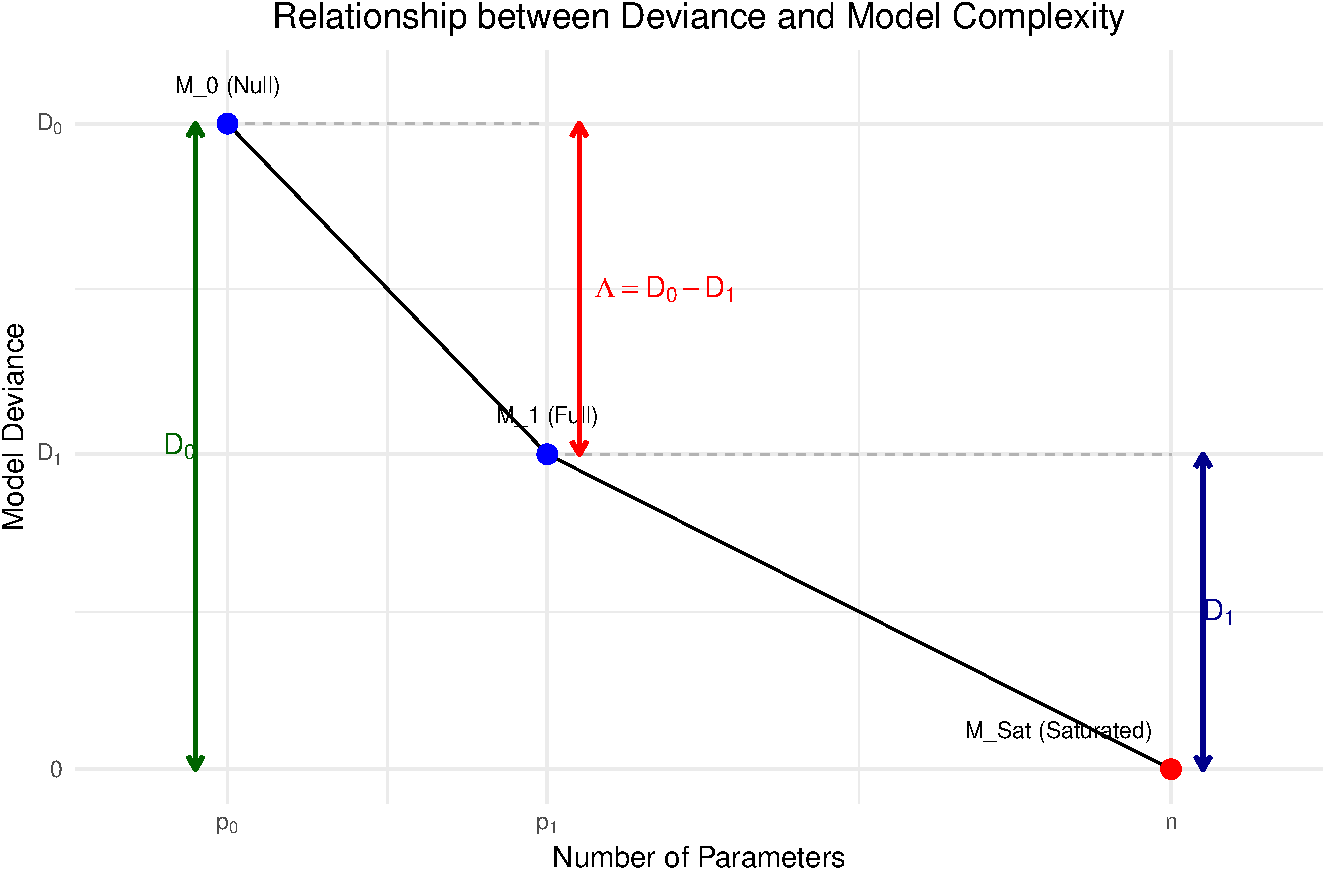
\includegraphics[keepaspectratio]{unit4-lr/logistic_files/figure-pdf/unnamed-chunk-6-1.pdf}}

As the diagram illustrates, the null model (\(M_0\)) has fewer
parameters (\(p_0\)) and a higher deviance (\(D_0\), or worse fit),
while the full model (\(M_1\)) has more parameters (\(p_1\)) and a lower
deviance (\(D_1\)). The Likelihood Ratio Test statistic \(D\) is the
magnitude of this drop in deviance.

For assessing the overall significance of a regression model
(\texttt{fit1\_chd}), this involves comparing it to its corresponding
intercept-only (null) model. The degrees of freedom for the \(\chi^2\)
test is the difference in the number of parameters, \(df = p_1 - p_0\),
which equals the number of predictors in the full model.

Here is an R code chunk demonstrating how to compute this p-value
directly from a \texttt{glm} fit object, assuming it is named
\texttt{fit1\_chd}.

\begin{Shaded}
\begin{Highlighting}[]
\CommentTok{\# Calculate the Likelihood Ratio Test statistic (D) and degrees of freedom (df)}
\CommentTok{\# by comparing the model\textquotesingle{}s deviance to the null (intercept{-}only) deviance,}
\CommentTok{\# both of which are stored in the \textquotesingle{}fit1\_chd\textquotesingle{} object.}
\FunctionTok{summary}\NormalTok{(fit1\_chd)}
\end{Highlighting}
\end{Shaded}

\begin{verbatim}

Call:
glm(formula = chd ~ smk + cat + sbp + age + chl + ecg + hpt, 
    family = binomial(link = "logit"), data = CHD.data)

Coefficients:
             Estimate Std. Error z value Pr(>|z|)    
(Intercept) -6.048892   1.345165  -4.497  6.9e-06 ***
smk          0.855951   0.306505   2.793  0.00523 ** 
cat          0.732763   0.376129   1.948  0.05139 .  
sbp         -0.006995   0.006976  -1.003  0.31600    
age          0.033956   0.015344   2.213  0.02690 *  
chl          0.008970   0.003274   2.740  0.00615 ** 
ecg          0.417776   0.295553   1.414  0.15750    
hpt          0.655498   0.359976   1.821  0.06861 .  
---
Signif. codes:  0 '***' 0.001 '**' 0.01 '*' 0.05 '.' 0.1 ' ' 1

(Dispersion parameter for binomial family taken to be 1)

    Null deviance: 438.56  on 608  degrees of freedom
Residual deviance: 399.35  on 601  degrees of freedom
AIC: 415.35

Number of Fisher Scoring iterations: 5
\end{verbatim}

\begin{Shaded}
\begin{Highlighting}[]
\NormalTok{lrt\_statistic }\OtherTok{\textless{}{-}}\NormalTok{ fit1\_chd}\SpecialCharTok{$}\NormalTok{null.deviance }\SpecialCharTok{{-}}\NormalTok{ fit1\_chd}\SpecialCharTok{$}\NormalTok{deviance}
\NormalTok{lrt\_df }\OtherTok{\textless{}{-}}\NormalTok{ fit1\_chd}\SpecialCharTok{$}\NormalTok{df.null }\SpecialCharTok{{-}}\NormalTok{ fit1\_chd}\SpecialCharTok{$}\NormalTok{df.residual}

\CommentTok{\# Compute the p{-}value from the chi{-}squared distribution}
\CommentTok{\# We use lower.tail = FALSE to get P(ChiSq \textgreater{} D)}
\NormalTok{p\_value }\OtherTok{\textless{}{-}} \FunctionTok{pchisq}\NormalTok{(lrt\_statistic, lrt\_df, }\AttributeTok{lower.tail =} \ConstantTok{FALSE}\NormalTok{)}

\CommentTok{\# Create and print the result in an ANOVA{-}like table}
\CommentTok{\# Row 1: Null model}
\CommentTok{\# Row 2: Full model (fit1\_chd), showing the test against the null}
\NormalTok{lrt\_table }\OtherTok{\textless{}{-}} \FunctionTok{data.frame}\NormalTok{(}
  \StringTok{"Resid. Df"} \OtherTok{=} \FunctionTok{c}\NormalTok{(fit1\_chd}\SpecialCharTok{$}\NormalTok{df.null, fit1\_chd}\SpecialCharTok{$}\NormalTok{df.residual),}
  \StringTok{"Resid. Dev"} \OtherTok{=} \FunctionTok{c}\NormalTok{(}\FunctionTok{round}\NormalTok{(fit1\_chd}\SpecialCharTok{$}\NormalTok{null.deviance, }\DecValTok{4}\NormalTok{), }\FunctionTok{round}\NormalTok{(fit1\_chd}\SpecialCharTok{$}\NormalTok{deviance, }\DecValTok{4}\NormalTok{)),}
  \StringTok{"Test Df"} \OtherTok{=} \FunctionTok{c}\NormalTok{(}\ConstantTok{NA}\NormalTok{, lrt\_df),}
  \StringTok{"Test Statistic (D)"} \OtherTok{=} \FunctionTok{c}\NormalTok{(}\ConstantTok{NA}\NormalTok{, }\FunctionTok{round}\NormalTok{(lrt\_statistic, }\DecValTok{4}\NormalTok{)),}
  \StringTok{"p{-}value"} \OtherTok{=} \FunctionTok{c}\NormalTok{(}\ConstantTok{NA}\NormalTok{, }\FunctionTok{format.pval}\NormalTok{(p\_value, }\AttributeTok{digits =} \DecValTok{4}\NormalTok{)),}
  \AttributeTok{row.names =} \FunctionTok{c}\NormalTok{(}\StringTok{"Null Model"}\NormalTok{, }\StringTok{"Full Model (fit1\_chd)"}\NormalTok{),}
  \AttributeTok{check.names =} \ConstantTok{FALSE} \CommentTok{\# Prevent R from changing \textquotesingle{}p{-}value\textquotesingle{} to \textquotesingle{}p.value\textquotesingle{}}
\NormalTok{)}

\FunctionTok{cat}\NormalTok{(}\StringTok{"Likelihood Ratio Test for Model Significance:}\SpecialCharTok{\textbackslash{}n}\StringTok{"}\NormalTok{)}
\end{Highlighting}
\end{Shaded}

\begin{verbatim}
Likelihood Ratio Test for Model Significance:
\end{verbatim}

\begin{Shaded}
\begin{Highlighting}[]
\NormalTok{lrt\_table}
\end{Highlighting}
\end{Shaded}

\begin{verbatim}
                      Resid. Df Resid. Dev Test Df Test Statistic (D)   p-value
Null Model                  608   438.5583      NA                 NA      <NA>
Full Model (fit1_chd)       601   399.3539       7            39.2044 1.787e-06
\end{verbatim}

\textbf{Using built-in anova() function}

\begin{Shaded}
\begin{Highlighting}[]
\NormalTok{fit0\_chd }\OtherTok{\textless{}{-}} \FunctionTok{glm}\NormalTok{ (chd}\SpecialCharTok{\textasciitilde{}}\DecValTok{1}\NormalTok{, }\AttributeTok{data =}\NormalTok{ CHD.data, }\AttributeTok{family =} \FunctionTok{binomial}\NormalTok{())}
\FunctionTok{anova}\NormalTok{(fit0\_chd, fit1\_chd)}
\end{Highlighting}
\end{Shaded}

\begin{verbatim}
Analysis of Deviance Table

Model 1: chd ~ 1
Model 2: chd ~ smk + cat + sbp + age + chl + ecg + hpt
  Resid. Df Resid. Dev Df Deviance  Pr(>Chi)    
1       608     438.56                          
2       601     399.35  7   39.204 1.787e-06 ***
---
Signif. codes:  0 '***' 0.001 '**' 0.01 '*' 0.05 '.' 0.1 ' ' 1
\end{verbatim}

\begin{Shaded}
\begin{Highlighting}[]
\FunctionTok{anova}\NormalTok{(fit1\_chd, }\AttributeTok{test=}\StringTok{"LRT"}\NormalTok{)}
\end{Highlighting}
\end{Shaded}

\begin{verbatim}
Analysis of Deviance Table

Model: binomial, link: logit

Response: chd

Terms added sequentially (first to last)

     Df Deviance Resid. Df Resid. Dev  Pr(>Chi)    
NULL                   608     438.56              
smk   1   5.7453       607     432.81 0.0165324 *  
cat   1  14.3716       606     418.44 0.0001501 ***
sbp   1   0.7574       605     417.68 0.3841353    
age   1   5.2821       604     412.40 0.0215455 *  
chl   1   7.8619       603     404.54 0.0050489 ** 
ecg   1   1.8701       602     402.67 0.1714609    
hpt   1   3.3159       601     399.35 0.0686113 .  
---
Signif. codes:  0 '***' 0.001 '**' 0.01 '*' 0.05 '.' 0.1 ' ' 1
\end{verbatim}

\section{\texorpdfstring{Assessing Predictive Effect-Size (Anologue to
\(R^2_\mathrm{adj}\))}{Assessing Predictive Effect-Size (Anologue to R\^{}2\_\textbackslash mathrm\{adj\})}}\label{assessing-predictive-effect-size-anologue-to-r2_mathrmadj}

While the LRT assesses overall model significance (in-sample fit), it's
also crucial to evaluate how well the model predicts new, unseen data
(out-of-sample performance). A common method is to split the data into a
training set (e.g., 2/3 of the data) and a test set (e.g., 1/3). The
model is fit using only the training data and then used to make
predictions for the test data. We can then compare these predictions to
the actual outcomes in the test set.

\subsection{Understanding the Confusion Matrix and
Metrics}\label{understanding-the-confusion-matrix-and-metrics}

To evaluate a model's predictive performance, we classify its
probabilistic predictions using a threshold (typically 0.5) and compare
them to the true outcomes in a \textbf{Confusion Matrix}:

\begin{longtable}[]{@{}lll@{}}
\toprule\noalign{}
& \textbf{Predicted: 0} & \textbf{Predicted: 1} \\
\midrule\noalign{}
\endhead
\bottomrule\noalign{}
\endlastfoot
\textbf{Actual: 0} & True Negative (TN) & False Positive (FP) \\
\textbf{Actual: 1} & False Negative (FN) & True Positive (TP) \\
\end{longtable}

From this matrix, we derive several key performance metrics:

\begin{itemize}
\item
  \textbf{Misclassification Error Rate (ER):} The proportion of all
  predictions that were incorrect. \[
    \text{Error Rate} = \frac{FP + FN}{TP + TN + FP + FN}
    \]
\item
  \textbf{Precision (Positive Predictive Value):} Answers: ``Of all the
  times the model predicted positive, how often was it correct?'' This
  is crucial when the cost of a \textbf{False Positive} is high. \[
    \text{Precision} = \frac{TP}{TP + FP}
    \]
\item
  \textbf{Recall (Sensitivity or True Positive Rate):} Answers: ``Of all
  the actual positive cases, how many did the model find?'' This is
  crucial when the cost of a \textbf{False Negative} is high. \[
    \text{Recall (TPR)} = \frac{TP}{TP + FN}
    \]
\item
  \textbf{ROC Curve and AUC:} An \textbf{ROC (Receiver Operating
  Characteristic) Curve} is a graph that shows a model's diagnostic
  ability across \emph{all possible classification thresholds}. It plots
  the \textbf{True Positive Rate (Recall)} on the y-axis against the
  \textbf{False Positive Rate} (FPR = \(\frac{FP}{FP + TN}\)) on the
  x-axis.

  \begin{itemize}
  \tightlist
  \item
    \textbf{Interpretation:} The curve shows the trade-off between
    sensitivity (finding all the positives) and specificity (not
    mislabeling negatives). A random ``no-skill'' classifier is
    represented by a diagonal line from (0,0) to (1,1). A perfect
    classifier would hug the \textbf{top-left corner} (TPR = 1, FPR =
    0).
  \item
    \textbf{AUC (Area Under the Curve):} The AUC summarizes the entire
    curve into a single number from 0 to 1. An AUC of 0.5 corresponds to
    a random guess, while an AUC of 1.0 represents a perfect model.
  \end{itemize}
\item
  \textbf{Precision-Recall (PR) Curve:} A \textbf{PR Curve} plots
  \textbf{Precision} (y-axis) against \textbf{Recall} (x-axis) at all
  possible thresholds.

  \begin{itemize}
  \tightlist
  \item
    \textbf{Interpretation:} This curve shows the trade-off between how
    \emph{reliable} a positive prediction is (Precision) and how
    \emph{complete} the model is at finding all positives (Recall).
  \item
    \textbf{When to Use:} The PR curve is particularly informative when
    the dataset is \textbf{imbalanced} (i.e., one class, like ``fraud''
    or ``disease,'' is much rarer than the other). Unlike the ROC curve,
    the PR curve's baseline (the ``no-skill'' line) is a horizontal line
    at the proportion of positive cases, which makes it easier to see if
    the model is performing significantly better than chance in a
    low-positive-rate scenario. A perfect classifier would hug the
    \textbf{top-right corner} (Precision = 1, Recall = 1).
  \end{itemize}
\end{itemize}

\subsection{Illustration with the Simulated
Dataset}\label{illustration-with-the-simulated-dataset}

This section applies the train/test split and model evaluation workflow
to the \texttt{sim.data} created in the previous step.

\begin{Shaded}
\begin{Highlighting}[]
\CommentTok{\# Load the pROC library for AUC calculation}
\CommentTok{\# install.packages("pROC") \# Uncomment to install if needed}
\FunctionTok{library}\NormalTok{(pROC)}

\CommentTok{\# {-}{-}{-} 1. Split the data {-}{-}{-}}
\CommentTok{\# We use \textquotesingle{}sim.data\textquotesingle{} which has 200 rows}
\FunctionTok{set.seed}\NormalTok{(}\DecValTok{123}\NormalTok{) }\CommentTok{\# for reproducibility}
\NormalTok{n\_sim }\OtherTok{\textless{}{-}} \FunctionTok{nrow}\NormalTok{(sim.data)}
\NormalTok{train\_size\_sim }\OtherTok{\textless{}{-}} \FunctionTok{floor}\NormalTok{(}\DecValTok{2}\SpecialCharTok{/}\DecValTok{3} \SpecialCharTok{*}\NormalTok{ n\_sim)}
\NormalTok{train\_indices\_sim }\OtherTok{\textless{}{-}} \FunctionTok{sample}\NormalTok{(}\DecValTok{1}\SpecialCharTok{:}\NormalTok{n\_sim, }\AttributeTok{size =}\NormalTok{ train\_size\_sim)}
\NormalTok{train\_data\_sim }\OtherTok{\textless{}{-}}\NormalTok{ sim.data[train\_indices\_sim, ]}
\NormalTok{test\_data\_sim  }\OtherTok{\textless{}{-}}\NormalTok{ sim.data[}\SpecialCharTok{{-}}\NormalTok{train\_indices\_sim, ]}

\CommentTok{\# {-}{-}{-} 2. Refit the model on the training data {-}{-}{-}}
\CommentTok{\# We fit the model y \textasciitilde{} x on the training data}
\NormalTok{fit\_train\_sim }\OtherTok{\textless{}{-}} \FunctionTok{glm}\NormalTok{(}
\NormalTok{  y }\SpecialCharTok{\textasciitilde{}}\NormalTok{ x,}
  \AttributeTok{data =}\NormalTok{ train\_data\_sim,}
  \AttributeTok{family =} \FunctionTok{binomial}\NormalTok{(}\AttributeTok{link =} \StringTok{"logit"}\NormalTok{)}
\NormalTok{)}

\CommentTok{\# {-}{-}{-} 3. Make predictions on the test data {-}{-}{-}}
\CommentTok{\# Note: The true probabilities \textquotesingle{}p\textquotesingle{} are also in test\_data\_sim}
\CommentTok{\# We predict from the *fitted* model}
\NormalTok{pred\_probs\_sim }\OtherTok{\textless{}{-}} \FunctionTok{predict}\NormalTok{(fit\_train\_sim, }\AttributeTok{newdata =}\NormalTok{ test\_data\_sim, }\AttributeTok{type =} \StringTok{"response"}\NormalTok{)}
\end{Highlighting}
\end{Shaded}

\textbf{Plotting the Predictive Probabilities with True Labels}

\begin{Shaded}
\begin{Highlighting}[]
\CommentTok{\# {-}{-}{-} 5. Plot sorted predicted probabilities {-}{-}{-}}

\CommentTok{\# Create a data frame for plotting}
\NormalTok{plot\_data\_sim }\OtherTok{\textless{}{-}} \FunctionTok{data.frame}\NormalTok{(}
  \AttributeTok{Prob =}\NormalTok{ pred\_probs\_sim,}
  \AttributeTok{Actual =} \FunctionTok{as.factor}\NormalTok{(test\_data\_sim}\SpecialCharTok{$}\NormalTok{y),}
  \AttributeTok{TrueProb =}\NormalTok{ test\_data\_sim}\SpecialCharTok{$}\NormalTok{p }\CommentTok{\# Include true probs for comparison}
\NormalTok{)}

\CommentTok{\# Sort by predicted probability}
\NormalTok{plot\_data\_sim }\OtherTok{\textless{}{-}}\NormalTok{ plot\_data\_sim[}\FunctionTok{order}\NormalTok{(plot\_data\_sim}\SpecialCharTok{$}\NormalTok{Prob), ]}
\NormalTok{plot\_data\_sim}\SpecialCharTok{$}\NormalTok{Rank }\OtherTok{\textless{}{-}} \DecValTok{1}\SpecialCharTok{:}\FunctionTok{nrow}\NormalTok{(plot\_data\_sim)}

\CommentTok{\# Create the plot}
\FunctionTok{plot}\NormalTok{(}
\NormalTok{  plot\_data\_sim}\SpecialCharTok{$}\NormalTok{Rank,}
\NormalTok{  plot\_data\_sim}\SpecialCharTok{$}\NormalTok{Prob,}
  \AttributeTok{pch =} \FunctionTok{ifelse}\NormalTok{(plot\_data\_sim}\SpecialCharTok{$}\NormalTok{Actual }\SpecialCharTok{==} \DecValTok{0}\NormalTok{, }\DecValTok{1}\NormalTok{, }\DecValTok{4}\NormalTok{),}
  \AttributeTok{col =} \FunctionTok{ifelse}\NormalTok{(plot\_data\_sim}\SpecialCharTok{$}\NormalTok{Actual }\SpecialCharTok{==} \DecValTok{0}\NormalTok{, }\StringTok{"blue"}\NormalTok{, }\StringTok{"red"}\NormalTok{),}
  \AttributeTok{xlab =} \StringTok{"Index (Sorted by Predicted Probability)"}\NormalTok{,}
  \AttributeTok{ylab =} \StringTok{"Predicted Probability"}\NormalTok{,}
  \AttributeTok{main =} \StringTok{"Predicted Probabilities vs. Actual Class (Simulated Data)"}\NormalTok{,}
  \AttributeTok{ylim =} \FunctionTok{c}\NormalTok{(}\DecValTok{0}\NormalTok{, }\DecValTok{1}\NormalTok{)}
\NormalTok{)}
\FunctionTok{abline}\NormalTok{(}\AttributeTok{h =} \FloatTok{0.5}\NormalTok{, }\AttributeTok{lty =} \DecValTok{2}\NormalTok{, }\AttributeTok{col =} \StringTok{"black"}\NormalTok{)}
\FunctionTok{abline}\NormalTok{(}\AttributeTok{h =} \FloatTok{0.1}\NormalTok{, }\AttributeTok{lty =} \DecValTok{3}\NormalTok{, }\AttributeTok{col =} \StringTok{"grey"}\NormalTok{)}

\CommentTok{\# Add the true probability curve (sorted by predicted prob)}
\CommentTok{\# This shows how well the fitted model\textquotesingle{}s predictions align with the true probs}
\CommentTok{\#lines(plot\_data\_sim$Rank, plot\_data\_sim$TrueProb[order(plot\_data\_sim$Prob)], col = "darkgreen", lwd = 2)}


\CommentTok{\# Add a legend}
\FunctionTok{legend}\NormalTok{(}
  \StringTok{"topleft"}\NormalTok{,}
  \AttributeTok{legend =} \FunctionTok{c}\NormalTok{(}\StringTok{"Actual 0 (o)"}\NormalTok{, }\StringTok{"Actual 1 (x)"}\NormalTok{),}
  \AttributeTok{pch =} \FunctionTok{c}\NormalTok{(}\DecValTok{1}\NormalTok{, }\DecValTok{4}\NormalTok{),}
  \AttributeTok{lty =} \FunctionTok{c}\NormalTok{(}\ConstantTok{NA}\NormalTok{, }\ConstantTok{NA}\NormalTok{),}
  \AttributeTok{lwd =} \FunctionTok{c}\NormalTok{(}\ConstantTok{NA}\NormalTok{, }\ConstantTok{NA}\NormalTok{),}
  \AttributeTok{col =} \FunctionTok{c}\NormalTok{(}\StringTok{"blue"}\NormalTok{, }\StringTok{"red"}\NormalTok{)}
\NormalTok{)}
\end{Highlighting}
\end{Shaded}

\pandocbounded{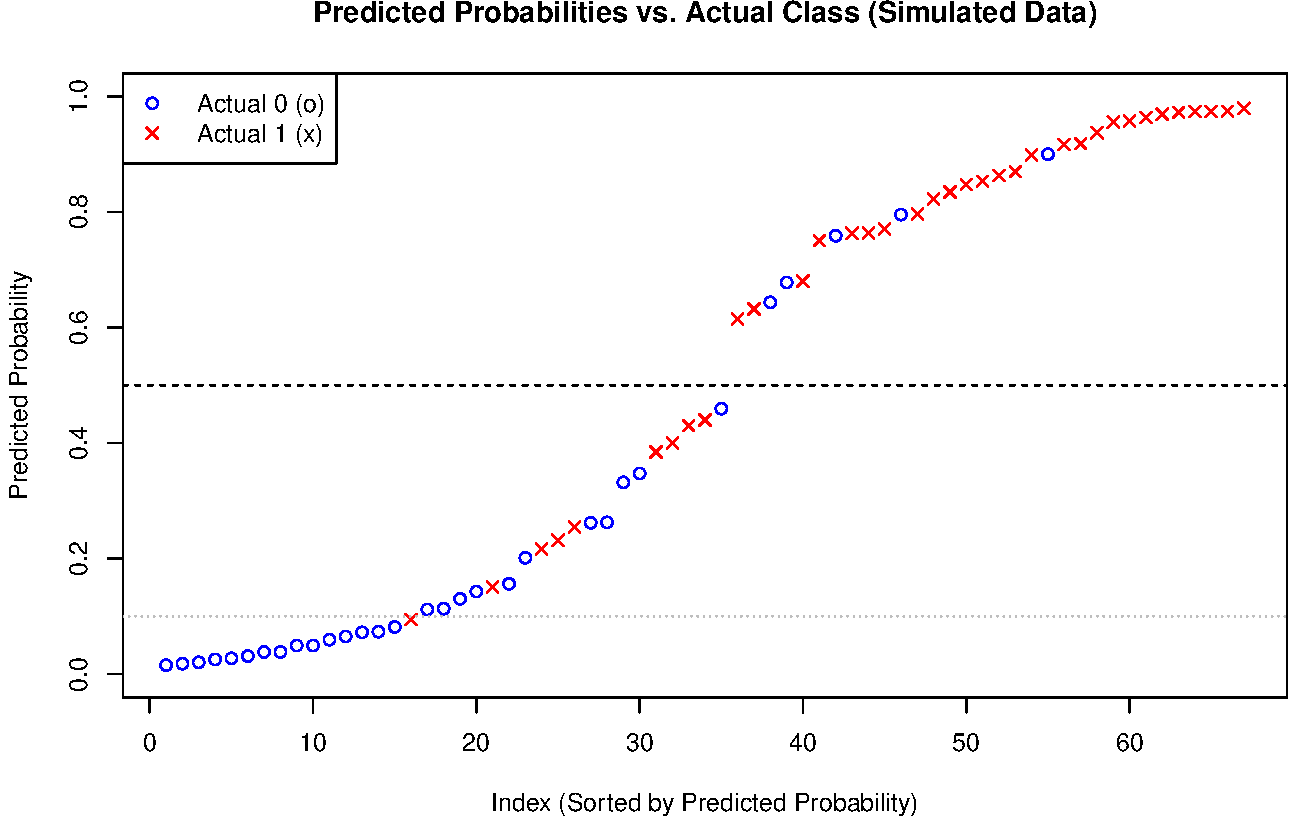
\includegraphics[keepaspectratio]{unit4-lr/logistic_files/figure-pdf/plot-sorted-probabilities-sim-1.pdf}}

\textbf{Confusion Matrix with threshold=0.5}

\begin{Shaded}
\begin{Highlighting}[]
\CommentTok{\# {-}{-}{-} 4. Assess accuracy {-}{-}{-}}

\CommentTok{\# 4a. Misclassification Error Rate (using 0.5 threshold)}
\NormalTok{threshold }\OtherTok{\textless{}{-}} \FloatTok{0.5}
\NormalTok{pred\_class\_sim }\OtherTok{\textless{}{-}} \FunctionTok{ifelse}\NormalTok{(pred\_probs\_sim }\SpecialCharTok{\textgreater{}}\NormalTok{ threshold, }\DecValTok{1}\NormalTok{, }\DecValTok{0}\NormalTok{)}
\NormalTok{conf\_matrix\_sim }\OtherTok{\textless{}{-}} \FunctionTok{table}\NormalTok{(}\AttributeTok{Actual =}\NormalTok{ test\_data\_sim}\SpecialCharTok{$}\NormalTok{y, }\AttributeTok{Predicted =}\NormalTok{ pred\_class\_sim)}

\CommentTok{\# {-}{-}{-} MODIFIED LINES START {-}{-}{-}}
\FunctionTok{cat}\NormalTok{(}\StringTok{"Confusion Matrix (Counts, threshold = 0.5):}\SpecialCharTok{\textbackslash{}n}\StringTok{"}\NormalTok{)}
\end{Highlighting}
\end{Shaded}

\begin{verbatim}
Confusion Matrix (Counts, threshold = 0.5):
\end{verbatim}

\begin{Shaded}
\begin{Highlighting}[]
\FunctionTok{print}\NormalTok{(conf\_matrix\_sim)}
\end{Highlighting}
\end{Shaded}

\begin{verbatim}
      Predicted
Actual  0  1
     0 26  5
     1  9 27
\end{verbatim}

\begin{Shaded}
\begin{Highlighting}[]
\FunctionTok{cat}\NormalTok{(}\StringTok{"}\SpecialCharTok{\textbackslash{}n}\StringTok{Row Proportions (Given Actual, \% Predicted {-}{-} Relates to TPR/FPR):}\SpecialCharTok{\textbackslash{}n}\StringTok{"}\NormalTok{)}
\end{Highlighting}
\end{Shaded}

\begin{verbatim}

Row Proportions (Given Actual, % Predicted -- Relates to TPR/FPR):
\end{verbatim}

\begin{Shaded}
\begin{Highlighting}[]
\CommentTok{\# margin = 1 calculates proportions across rows}
\FunctionTok{print}\NormalTok{(}\FunctionTok{round}\NormalTok{(}\FunctionTok{prop.table}\NormalTok{(conf\_matrix\_sim, }\AttributeTok{margin =} \DecValTok{1}\NormalTok{), }\DecValTok{3}\NormalTok{))}
\end{Highlighting}
\end{Shaded}

\begin{verbatim}
      Predicted
Actual     0     1
     0 0.839 0.161
     1 0.250 0.750
\end{verbatim}

\begin{Shaded}
\begin{Highlighting}[]
\FunctionTok{cat}\NormalTok{(}\StringTok{"}\SpecialCharTok{\textbackslash{}n}\StringTok{Column Proportions (Given Predicted, \% Actual {-}{-} Relates to Precision):}\SpecialCharTok{\textbackslash{}n}\StringTok{"}\NormalTok{)}
\end{Highlighting}
\end{Shaded}

\begin{verbatim}

Column Proportions (Given Predicted, % Actual -- Relates to Precision):
\end{verbatim}

\begin{Shaded}
\begin{Highlighting}[]
\CommentTok{\# margin = 2 calculates proportions across columns}
\FunctionTok{print}\NormalTok{(}\FunctionTok{round}\NormalTok{(}\FunctionTok{prop.table}\NormalTok{(conf\_matrix\_sim, }\AttributeTok{margin =} \DecValTok{2}\NormalTok{), }\DecValTok{3}\NormalTok{))}
\end{Highlighting}
\end{Shaded}

\begin{verbatim}
      Predicted
Actual     0     1
     0 0.743 0.156
     1 0.257 0.844
\end{verbatim}

\begin{Shaded}
\begin{Highlighting}[]
\CommentTok{\# {-}{-}{-} MODIFIED LINES }\RegionMarkerTok{END}\CommentTok{ {-}{-}{-}}


\CommentTok{\# Check if matrix has 2x2 dimensions, otherwise metrics will fail}
\ControlFlowTok{if}\NormalTok{ (}\FunctionTok{all}\NormalTok{(}\FunctionTok{dim}\NormalTok{(conf\_matrix\_sim) }\SpecialCharTok{==} \FunctionTok{c}\NormalTok{(}\DecValTok{2}\NormalTok{, }\DecValTok{2}\NormalTok{))) \{}
\NormalTok{  TN }\OtherTok{\textless{}{-}}\NormalTok{ conf\_matrix\_sim[}\DecValTok{1}\NormalTok{, }\DecValTok{1}\NormalTok{]}
\NormalTok{  FP }\OtherTok{\textless{}{-}}\NormalTok{ conf\_matrix\_sim[}\DecValTok{1}\NormalTok{, }\DecValTok{2}\NormalTok{]}
\NormalTok{  FN }\OtherTok{\textless{}{-}}\NormalTok{ conf\_matrix\_sim[}\DecValTok{2}\NormalTok{, }\DecValTok{1}\NormalTok{]}
\NormalTok{  TP }\OtherTok{\textless{}{-}}\NormalTok{ conf\_matrix\_sim[}\DecValTok{2}\NormalTok{, }\DecValTok{2}\NormalTok{]}

  \CommentTok{\# Calculate metrics}
\NormalTok{  error\_rate }\OtherTok{\textless{}{-}}\NormalTok{ (FP }\SpecialCharTok{+}\NormalTok{ FN) }\SpecialCharTok{/}\NormalTok{ (TP }\SpecialCharTok{+}\NormalTok{ TN }\SpecialCharTok{+}\NormalTok{ FP }\SpecialCharTok{+}\NormalTok{ FN)}
\NormalTok{  TPR\_Recall }\OtherTok{\textless{}{-}}\NormalTok{ TP }\SpecialCharTok{/}\NormalTok{ (TP }\SpecialCharTok{+}\NormalTok{ FN) }\CommentTok{\# True Positive Rate (Recall / Sensitivity)}
\NormalTok{  FPR }\OtherTok{\textless{}{-}}\NormalTok{ FP }\SpecialCharTok{/}\NormalTok{ (FP }\SpecialCharTok{+}\NormalTok{ TN)      }\CommentTok{\# False Positive Rate (1 {-} Specificity)}
\NormalTok{  Precision }\OtherTok{\textless{}{-}}\NormalTok{ TP }\SpecialCharTok{/}\NormalTok{ (TP }\SpecialCharTok{+}\NormalTok{ FP)  }\CommentTok{\# Positive Predictive Value}

  \FunctionTok{cat}\NormalTok{(}\FunctionTok{paste}\NormalTok{(}\StringTok{"}\SpecialCharTok{\textbackslash{}n}\StringTok{Misclassification Error Rate:"}\NormalTok{, }\FunctionTok{round}\NormalTok{(error\_rate, }\DecValTok{4}\NormalTok{), }\StringTok{"}\SpecialCharTok{\textbackslash{}n}\StringTok{"}\NormalTok{))}
  \FunctionTok{cat}\NormalTok{(}\FunctionTok{paste}\NormalTok{(}\StringTok{"True Positive Rate (Recall):"}\NormalTok{, }\FunctionTok{round}\NormalTok{(TPR\_Recall, }\DecValTok{4}\NormalTok{), }\StringTok{"}\SpecialCharTok{\textbackslash{}n}\StringTok{"}\NormalTok{))}
  \FunctionTok{cat}\NormalTok{(}\FunctionTok{paste}\NormalTok{(}\StringTok{"False Positive Rate:"}\NormalTok{, }\FunctionTok{round}\NormalTok{(FPR, }\DecValTok{4}\NormalTok{), }\StringTok{"}\SpecialCharTok{\textbackslash{}n}\StringTok{"}\NormalTok{))}
  \FunctionTok{cat}\NormalTok{(}\FunctionTok{paste}\NormalTok{(}\StringTok{"Precision:"}\NormalTok{, }\FunctionTok{round}\NormalTok{(Precision, }\DecValTok{4}\NormalTok{), }\StringTok{"}\SpecialCharTok{\textbackslash{}n}\StringTok{"}\NormalTok{))}
\NormalTok{\} }\ControlFlowTok{else}\NormalTok{ \{}
  \FunctionTok{cat}\NormalTok{(}\StringTok{"}\SpecialCharTok{\textbackslash{}n}\StringTok{Cannot calculate full metrics: model predicted only one class.}\SpecialCharTok{\textbackslash{}n}\StringTok{"}\NormalTok{)}
\NormalTok{\}}
\end{Highlighting}
\end{Shaded}

\begin{verbatim}

Misclassification Error Rate: 0.209 
True Positive Rate (Recall): 0.75 
False Positive Rate: 0.1613 
Precision: 0.8438 
\end{verbatim}

\textbf{Confusion Matrix with threshold=0.1}

\begin{Shaded}
\begin{Highlighting}[]
\NormalTok{threshold }\OtherTok{\textless{}{-}} \FloatTok{0.1}
\NormalTok{pred\_class\_sim }\OtherTok{\textless{}{-}} \FunctionTok{ifelse}\NormalTok{(pred\_probs\_sim }\SpecialCharTok{\textgreater{}}\NormalTok{ threshold, }\DecValTok{1}\NormalTok{, }\DecValTok{0}\NormalTok{)}
\NormalTok{conf\_matrix\_sim }\OtherTok{\textless{}{-}} \FunctionTok{table}\NormalTok{(}\AttributeTok{Actual =}\NormalTok{ test\_data\_sim}\SpecialCharTok{$}\NormalTok{y, }\AttributeTok{Predicted =}\NormalTok{ pred\_class\_sim)}

\CommentTok{\# {-}{-}{-} MODIFIED LINES START {-}{-}{-}}
\FunctionTok{cat}\NormalTok{(}\StringTok{"Confusion Matrix (Counts, threshold = 0.1):}\SpecialCharTok{\textbackslash{}n}\StringTok{"}\NormalTok{)}
\end{Highlighting}
\end{Shaded}

\begin{verbatim}
Confusion Matrix (Counts, threshold = 0.1):
\end{verbatim}

\begin{Shaded}
\begin{Highlighting}[]
\FunctionTok{print}\NormalTok{(conf\_matrix\_sim)}
\end{Highlighting}
\end{Shaded}

\begin{verbatim}
      Predicted
Actual  0  1
     0 15 16
     1  1 35
\end{verbatim}

\begin{Shaded}
\begin{Highlighting}[]
\FunctionTok{cat}\NormalTok{(}\StringTok{"}\SpecialCharTok{\textbackslash{}n}\StringTok{Row Proportions (Given Actual, \% Predicted {-}{-} Relates to TPR/FPR):}\SpecialCharTok{\textbackslash{}n}\StringTok{"}\NormalTok{)}
\end{Highlighting}
\end{Shaded}

\begin{verbatim}

Row Proportions (Given Actual, % Predicted -- Relates to TPR/FPR):
\end{verbatim}

\begin{Shaded}
\begin{Highlighting}[]
\CommentTok{\# margin = 1 calculates proportions across rows}
\FunctionTok{print}\NormalTok{(}\FunctionTok{round}\NormalTok{(}\FunctionTok{prop.table}\NormalTok{(conf\_matrix\_sim, }\AttributeTok{margin =} \DecValTok{1}\NormalTok{), }\DecValTok{3}\NormalTok{))}
\end{Highlighting}
\end{Shaded}

\begin{verbatim}
      Predicted
Actual     0     1
     0 0.484 0.516
     1 0.028 0.972
\end{verbatim}

\begin{Shaded}
\begin{Highlighting}[]
\FunctionTok{cat}\NormalTok{(}\StringTok{"}\SpecialCharTok{\textbackslash{}n}\StringTok{Column Proportions (Given Predicted, \% Actual {-}{-} Relates to Precision):}\SpecialCharTok{\textbackslash{}n}\StringTok{"}\NormalTok{)}
\end{Highlighting}
\end{Shaded}

\begin{verbatim}

Column Proportions (Given Predicted, % Actual -- Relates to Precision):
\end{verbatim}

\begin{Shaded}
\begin{Highlighting}[]
\CommentTok{\# margin = 2 calculates proportions across columns}
\FunctionTok{print}\NormalTok{(}\FunctionTok{round}\NormalTok{(}\FunctionTok{prop.table}\NormalTok{(conf\_matrix\_sim, }\AttributeTok{margin =} \DecValTok{2}\NormalTok{), }\DecValTok{3}\NormalTok{))}
\end{Highlighting}
\end{Shaded}

\begin{verbatim}
      Predicted
Actual     0     1
     0 0.938 0.314
     1 0.062 0.686
\end{verbatim}

\begin{Shaded}
\begin{Highlighting}[]
\CommentTok{\# {-}{-}{-} MODIFIED LINES }\RegionMarkerTok{END}\CommentTok{ {-}{-}{-}}


\CommentTok{\# Check if matrix has 2x2 dimensions}
\ControlFlowTok{if}\NormalTok{ (}\FunctionTok{all}\NormalTok{(}\FunctionTok{dim}\NormalTok{(conf\_matrix\_sim) }\SpecialCharTok{==} \FunctionTok{c}\NormalTok{(}\DecValTok{2}\NormalTok{, }\DecValTok{2}\NormalTok{))) \{}
\NormalTok{  TN }\OtherTok{\textless{}{-}}\NormalTok{ conf\_matrix\_sim[}\DecValTok{1}\NormalTok{, }\DecValTok{1}\NormalTok{]}
\NormalTok{  FP }\OtherTok{\textless{}{-}}\NormalTok{ conf\_matrix\_sim[}\DecValTok{1}\NormalTok{, }\DecValTok{2}\NormalTok{]}
\NormalTok{  FN }\OtherTok{\textless{}{-}}\NormalTok{ conf\_matrix\_sim[}\DecValTok{2}\NormalTok{, }\DecValTok{1}\NormalTok{]}
\NormalTok{  TP }\OtherTok{\textless{}{-}}\NormalTok{ conf\_matrix\_sim[}\DecValTok{2}\NormalTok{, }\DecValTok{2}\NormalTok{]}

  \CommentTok{\# Calculate metrics}
\NormalTok{  error\_rate }\OtherTok{\textless{}{-}}\NormalTok{ (FP }\SpecialCharTok{+}\NormalTok{ FN) }\SpecialCharTok{/}\NormalTok{ (TP }\SpecialCharTok{+}\NormalTok{ TN }\SpecialCharTok{+}\NormalTok{ FP }\SpecialCharTok{+}\NormalTok{ FN)}
\NormalTok{  TPR\_Recall }\OtherTok{\textless{}{-}}\NormalTok{ TP }\SpecialCharTok{/}\NormalTok{ (TP }\SpecialCharTok{+}\NormalTok{ FN) }\CommentTok{\# True Positive Rate (Recall / Sensitivity)}
\NormalTok{  FPR }\OtherTok{\textless{}{-}}\NormalTok{ FP }\SpecialCharTok{/}\NormalTok{ (FP }\SpecialCharTok{+}\NormalTok{ TN)      }\CommentTok{\# False Positive Rate (1 {-} Specificity)}
\NormalTok{  Precision }\OtherTok{\textless{}{-}}\NormalTok{ TP }\SpecialCharTok{/}\NormalTok{ (TP }\SpecialCharTok{+}\NormalTok{ FP)  }\CommentTok{\# Positive Predictive Value}

  \FunctionTok{cat}\NormalTok{(}\FunctionTok{paste}\NormalTok{(}\StringTok{"}\SpecialCharTok{\textbackslash{}n}\StringTok{Misclassification Error Rate:"}\NormalTok{, }\FunctionTok{round}\NormalTok{(error\_rate, }\DecValTok{4}\NormalTok{), }\StringTok{"}\SpecialCharTok{\textbackslash{}n}\StringTok{"}\NormalTok{))}
  \FunctionTok{cat}\NormalTok{(}\FunctionTok{paste}\NormalTok{(}\StringTok{"True Positive Rate (Recall):"}\NormalTok{, }\FunctionTok{round}\NormalTok{(TPR\_Recall, }\DecValTok{4}\NormalTok{), }\StringTok{"}\SpecialCharTok{\textbackslash{}n}\StringTok{"}\NormalTok{))}
  \FunctionTok{cat}\NormalTok{(}\FunctionTok{paste}\NormalTok{(}\StringTok{"False Positive Rate:"}\NormalTok{, }\FunctionTok{round}\NormalTok{(FPR, }\DecValTok{4}\NormalTok{), }\StringTok{"}\SpecialCharTok{\textbackslash{}n}\StringTok{"}\NormalTok{))}
  \FunctionTok{cat}\NormalTok{(}\FunctionTok{paste}\NormalTok{(}\StringTok{"Precision:"}\NormalTok{, }\FunctionTok{round}\NormalTok{(Precision, }\DecValTok{4}\NormalTok{), }\StringTok{"}\SpecialCharTok{\textbackslash{}n}\StringTok{"}\NormalTok{))}
\NormalTok{\} }\ControlFlowTok{else}\NormalTok{ \{}
  \FunctionTok{cat}\NormalTok{(}\StringTok{"}\SpecialCharTok{\textbackslash{}n}\StringTok{Cannot calculate full metrics: model predicted only one class.}\SpecialCharTok{\textbackslash{}n}\StringTok{"}\NormalTok{)}
\NormalTok{\}}
\end{Highlighting}
\end{Shaded}

\begin{verbatim}

Misclassification Error Rate: 0.2537 
True Positive Rate (Recall): 0.9722 
False Positive Rate: 0.5161 
Precision: 0.6863 
\end{verbatim}

\textbf{ROC curve and Area Under the ROC (AUC)}

\begin{Shaded}
\begin{Highlighting}[]
\CommentTok{\# 4b. Area Under the Curve (AUC)}
\NormalTok{roc\_curve\_sim }\OtherTok{\textless{}{-}} \FunctionTok{roc}\NormalTok{(test\_data\_sim}\SpecialCharTok{$}\NormalTok{y, pred\_probs\_sim, }\AttributeTok{quiet =} \ConstantTok{TRUE}\NormalTok{)}

\CommentTok{\# Plot the ROC curve}
\FunctionTok{plot}\NormalTok{(roc\_curve\_sim, }\AttributeTok{main =} \StringTok{"ROC Curve (Simulated Test Data)"}\NormalTok{, }\AttributeTok{print.auc =} \ConstantTok{TRUE}\NormalTok{)}
\end{Highlighting}
\end{Shaded}

\pandocbounded{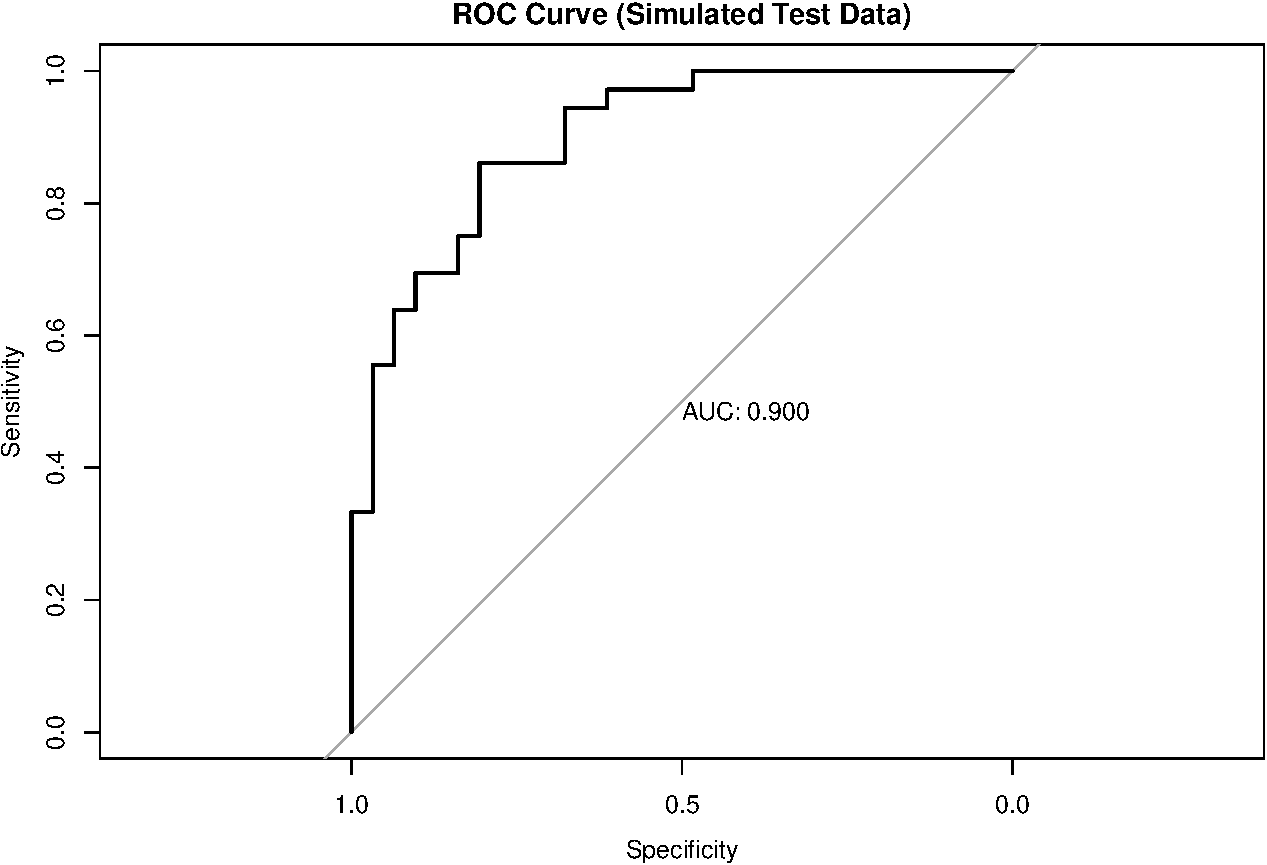
\includegraphics[keepaspectratio]{unit4-lr/logistic_files/figure-pdf/unnamed-chunk-8-1.pdf}}

\begin{Shaded}
\begin{Highlighting}[]
\NormalTok{auc\_value\_sim }\OtherTok{\textless{}{-}} \FunctionTok{auc}\NormalTok{(roc\_curve\_sim)}
\FunctionTok{cat}\NormalTok{(}\FunctionTok{paste}\NormalTok{(}\StringTok{"Area Under the Curve (AUC):"}\NormalTok{, }\FunctionTok{round}\NormalTok{(auc\_value\_sim, }\DecValTok{4}\NormalTok{), }\StringTok{"}\SpecialCharTok{\textbackslash{}n\textbackslash{}n}\StringTok{"}\NormalTok{))}
\end{Highlighting}
\end{Shaded}

\begin{verbatim}
Area Under the Curve (AUC): 0.8996 
\end{verbatim}

\textbf{PR curve and Area Under PR Curve (AUPR)}

\begin{Shaded}
\begin{Highlighting}[]
\CommentTok{\# Load the ROCR library}
\CommentTok{\# install.packages("ROCR") \# Uncomment to install if needed}
\FunctionTok{library}\NormalTok{(ROCR)}

\CommentTok{\# {-}{-}{-} 1. Create a \textquotesingle{}prediction\textquotesingle{} object {-}{-}{-}}
\CommentTok{\# \textquotesingle{}prediction\textquotesingle{} takes all predictions and all true labels}
\NormalTok{pred\_obj }\OtherTok{\textless{}{-}} \FunctionTok{prediction}\NormalTok{(pred\_probs\_sim, test\_data\_sim}\SpecialCharTok{$}\NormalTok{y)}

\CommentTok{\# {-}{-}{-} 2. Create a \textquotesingle{}performance\textquotesingle{} object for PR {-}{-}{-}}
\CommentTok{\# "prec" is for precision, "rec" is for recall}
\NormalTok{perf\_pr }\OtherTok{\textless{}{-}} \FunctionTok{performance}\NormalTok{(pred\_obj, }\AttributeTok{measure =} \StringTok{"prec"}\NormalTok{, }\AttributeTok{x.measure =} \StringTok{"rec"}\NormalTok{)}

\CommentTok{\# {-}{-}{-} 3. Calculate Area Under the PR Curve (AUPR) {-}{-}{-}}
\NormalTok{perf\_auc }\OtherTok{\textless{}{-}} \FunctionTok{performance}\NormalTok{(pred\_obj, }\AttributeTok{measure =} \StringTok{"aucpr"}\NormalTok{) }\CommentTok{\# "aucpr" = Area Under PR Curve}
\NormalTok{aupr\_value }\OtherTok{\textless{}{-}}\NormalTok{ perf\_auc}\SpecialCharTok{@}\NormalTok{y.values[[}\DecValTok{1}\NormalTok{]]}
\FunctionTok{cat}\NormalTok{(}\FunctionTok{paste}\NormalTok{(}\StringTok{"Area Under PR Curve (AUPR):"}\NormalTok{, }\FunctionTok{round}\NormalTok{(aupr\_value, }\DecValTok{4}\NormalTok{), }\StringTok{"}\SpecialCharTok{\textbackslash{}n}\StringTok{"}\NormalTok{))}
\end{Highlighting}
\end{Shaded}

\begin{verbatim}
Area Under PR Curve (AUPR): 0.9157 
\end{verbatim}

\begin{Shaded}
\begin{Highlighting}[]
\CommentTok{\# {-}{-}{-} 4. Plot the performance object {-}{-}{-}}
\FunctionTok{plot}\NormalTok{(perf\_pr, }
     \AttributeTok{main =} \StringTok{"Precision{-}Recall Curve (Simulated Test Data)"}\NormalTok{, }
     \AttributeTok{xlim =} \FunctionTok{c}\NormalTok{(}\DecValTok{0}\NormalTok{, }\DecValTok{1}\NormalTok{), }
     \AttributeTok{ylim =} \FunctionTok{c}\NormalTok{(}\DecValTok{0}\NormalTok{, }\DecValTok{1}\NormalTok{),}
     \AttributeTok{col =} \StringTok{"black"}\NormalTok{)}

\CommentTok{\# {-}{-}{-} 5. Calculate and add the \textquotesingle{}no{-}skill\textquotesingle{} baseline {-}{-}{-}}
\NormalTok{baseline\_precision\_sim }\OtherTok{\textless{}{-}} \FunctionTok{sum}\NormalTok{(test\_data\_sim}\SpecialCharTok{$}\NormalTok{y }\SpecialCharTok{==} \DecValTok{1}\NormalTok{) }\SpecialCharTok{/} \FunctionTok{length}\NormalTok{(test\_data\_sim}\SpecialCharTok{$}\NormalTok{y)}
\FunctionTok{abline}\NormalTok{(}\AttributeTok{h =}\NormalTok{ baseline\_precision\_sim, }\AttributeTok{col =} \StringTok{"blue"}\NormalTok{, }\AttributeTok{lty =} \DecValTok{2}\NormalTok{)}

\CommentTok{\# {-}{-}{-} 6. Add a legend with AUPR {-}{-}{-}}
\FunctionTok{legend}\NormalTok{(}\StringTok{"bottomleft"}\NormalTok{, }
       \AttributeTok{legend =} \FunctionTok{c}\NormalTok{(}
           \FunctionTok{paste}\NormalTok{(}\StringTok{"Model (AUPR ="}\NormalTok{, }\FunctionTok{round}\NormalTok{(aupr\_value, }\DecValTok{4}\NormalTok{), }\StringTok{")"}\NormalTok{),  }\CommentTok{\# \textless{}{-}{-} MODIFIED LINE}
           \FunctionTok{paste}\NormalTok{(}\StringTok{"Baseline ("}\NormalTok{, }\FunctionTok{round}\NormalTok{(baseline\_precision\_sim, }\DecValTok{3}\NormalTok{), }\StringTok{")"}\NormalTok{)}
\NormalTok{       ), }
       \AttributeTok{col =} \FunctionTok{c}\NormalTok{(}\StringTok{"black"}\NormalTok{, }\StringTok{"blue"}\NormalTok{), }
       \AttributeTok{lty =} \FunctionTok{c}\NormalTok{(}\DecValTok{1}\NormalTok{, }\DecValTok{2}\NormalTok{), }
       \AttributeTok{bty =} \StringTok{"n"}\NormalTok{) }\CommentTok{\# bty="n" removes the box}
\end{Highlighting}
\end{Shaded}

\pandocbounded{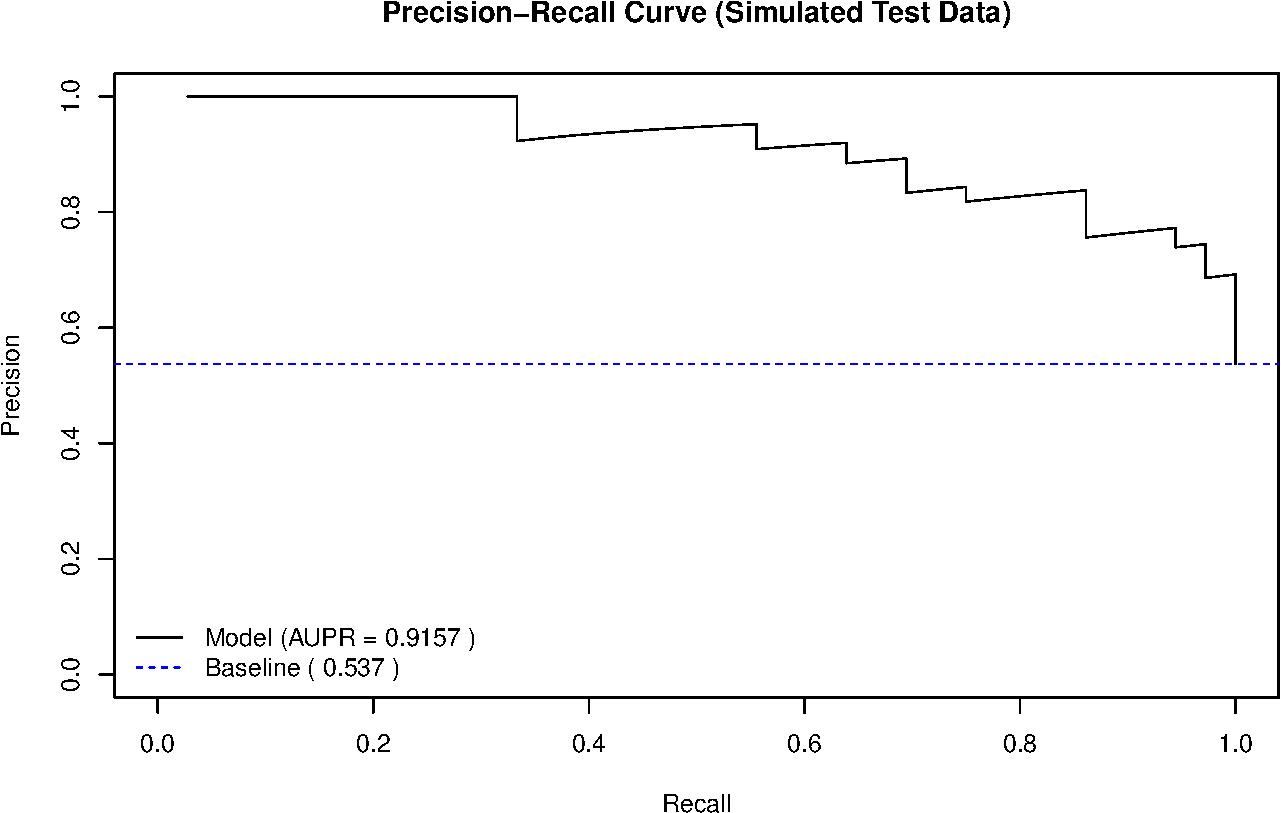
\includegraphics[keepaspectratio]{unit4-lr/logistic_files/figure-pdf/pr-curve-rocr-1.pdf}}

\subsection{Application to the CHD
Dataset}\label{application-to-the-chd-dataset}

\begin{Shaded}
\begin{Highlighting}[]
\CommentTok{\# Load the pROC library for AUC calculation}
\CommentTok{\# install.packages("pROC") \# Uncomment to install if needed}
\FunctionTok{library}\NormalTok{(pROC)}

\CommentTok{\# {-}{-}{-} 1. Split the data {-}{-}{-}}
\FunctionTok{set.seed}\NormalTok{(}\DecValTok{123}\NormalTok{) }\CommentTok{\# for reproducibility}
\NormalTok{n }\OtherTok{\textless{}{-}} \FunctionTok{nrow}\NormalTok{(CHD.data)}
\NormalTok{train\_size }\OtherTok{\textless{}{-}} \FunctionTok{floor}\NormalTok{(}\DecValTok{2}\SpecialCharTok{/}\DecValTok{3} \SpecialCharTok{*}\NormalTok{ n)}
\NormalTok{train\_indices }\OtherTok{\textless{}{-}} \FunctionTok{sample}\NormalTok{(}\DecValTok{1}\SpecialCharTok{:}\NormalTok{n, }\AttributeTok{size =}\NormalTok{ train\_size)}
\NormalTok{train\_data }\OtherTok{\textless{}{-}}\NormalTok{ CHD.data[train\_indices, ]}
\NormalTok{test\_data  }\OtherTok{\textless{}{-}}\NormalTok{ CHD.data[}\SpecialCharTok{{-}}\NormalTok{train\_indices, ]}

\CommentTok{\# {-}{-}{-} 2. Refit the model on the training data {-}{-}{-}}
\NormalTok{fit\_train }\OtherTok{\textless{}{-}} \FunctionTok{glm}\NormalTok{(}
\NormalTok{  chd }\SpecialCharTok{\textasciitilde{}}\NormalTok{ smk }\SpecialCharTok{+}\NormalTok{ cat }\SpecialCharTok{+}\NormalTok{ sbp }\SpecialCharTok{+}\NormalTok{ age }\SpecialCharTok{+}\NormalTok{ chl }\SpecialCharTok{+}\NormalTok{ ecg }\SpecialCharTok{+}\NormalTok{ hpt,}
  \AttributeTok{data =}\NormalTok{ train\_data,}
  \AttributeTok{family =} \FunctionTok{binomial}\NormalTok{(}\AttributeTok{link =} \StringTok{"logit"}\NormalTok{)}
\NormalTok{)}

\CommentTok{\# {-}{-}{-} 3. Make predictions on the test data {-}{-}{-}}
\NormalTok{pred\_probs }\OtherTok{\textless{}{-}} \FunctionTok{predict}\NormalTok{(fit\_train, }\AttributeTok{newdata =}\NormalTok{ test\_data, }\AttributeTok{type =} \StringTok{"response"}\NormalTok{)}
\end{Highlighting}
\end{Shaded}

\textbf{Plot Predictive Probabilities}

\begin{Shaded}
\begin{Highlighting}[]
\CommentTok{\# {-}{-}{-} 5. Plot sorted predicted probabilities {-}{-}{-}}

\CommentTok{\# Create a data frame for plotting}
\NormalTok{plot\_data }\OtherTok{\textless{}{-}} \FunctionTok{data.frame}\NormalTok{(}
  \AttributeTok{Prob =}\NormalTok{ pred\_probs,}
  \AttributeTok{Actual =} \FunctionTok{as.factor}\NormalTok{(test\_data}\SpecialCharTok{$}\NormalTok{chd)}
\NormalTok{)}

\CommentTok{\# Sort by predicted probability}
\NormalTok{plot\_data }\OtherTok{\textless{}{-}}\NormalTok{ plot\_data[}\FunctionTok{order}\NormalTok{(plot\_data}\SpecialCharTok{$}\NormalTok{Prob), ]}
\NormalTok{plot\_data}\SpecialCharTok{$}\NormalTok{Rank }\OtherTok{\textless{}{-}} \DecValTok{1}\SpecialCharTok{:}\FunctionTok{nrow}\NormalTok{(plot\_data)}

\CommentTok{\# Create the plot}
\CommentTok{\# We use \textquotesingle{}pch\textquotesingle{} (plot character) to set different symbols}
\CommentTok{\# \textquotesingle{}pch = 1\textquotesingle{} is \textquotesingle{}o\textquotesingle{} (default)}
\CommentTok{\# \textquotesingle{}pch = 4\textquotesingle{} is \textquotesingle{}x\textquotesingle{}}
\FunctionTok{plot}\NormalTok{(}
\NormalTok{  plot\_data}\SpecialCharTok{$}\NormalTok{Rank,}
\NormalTok{  plot\_data}\SpecialCharTok{$}\NormalTok{Prob,}
  \AttributeTok{pch =} \FunctionTok{ifelse}\NormalTok{(plot\_data}\SpecialCharTok{$}\NormalTok{Actual }\SpecialCharTok{==} \DecValTok{0}\NormalTok{, }\DecValTok{1}\NormalTok{, }\DecValTok{4}\NormalTok{),}
  \AttributeTok{col =} \FunctionTok{ifelse}\NormalTok{(plot\_data}\SpecialCharTok{$}\NormalTok{Actual }\SpecialCharTok{==} \DecValTok{0}\NormalTok{, }\StringTok{"blue"}\NormalTok{, }\StringTok{"red"}\NormalTok{),}
  \AttributeTok{xlab =} \StringTok{"Index (Sorted by Predicted Probability)"}\NormalTok{,}
  \AttributeTok{ylab =} \StringTok{"Log{-}odds of Predicted Probability"}\NormalTok{,}
  \AttributeTok{main =} \StringTok{"Predicted Probabilities vs. Actual Class"}\NormalTok{,}
  \AttributeTok{ylim =} \FunctionTok{c}\NormalTok{(}\DecValTok{0}\NormalTok{,}\DecValTok{1}\NormalTok{)}
\NormalTok{)}
\FunctionTok{abline}\NormalTok{(}\AttributeTok{h=}\FloatTok{0.5}\NormalTok{)}
\FunctionTok{abline}\NormalTok{(}\AttributeTok{h=}\FloatTok{0.1}\NormalTok{, }\AttributeTok{col=}\StringTok{"grey"}\NormalTok{)}

\CommentTok{\# Add a legend}
\FunctionTok{legend}\NormalTok{(}
  \StringTok{"topleft"}\NormalTok{,}
  \AttributeTok{legend =} \FunctionTok{c}\NormalTok{(}\StringTok{"Actual 0 (o)"}\NormalTok{, }\StringTok{"Actual 1 (x)"}\NormalTok{),}
  \AttributeTok{pch =} \FunctionTok{c}\NormalTok{(}\DecValTok{1}\NormalTok{, }\DecValTok{4}\NormalTok{),}
  \AttributeTok{col =} \FunctionTok{c}\NormalTok{(}\StringTok{"blue"}\NormalTok{, }\StringTok{"red"}\NormalTok{)}
\NormalTok{)}
\end{Highlighting}
\end{Shaded}

\pandocbounded{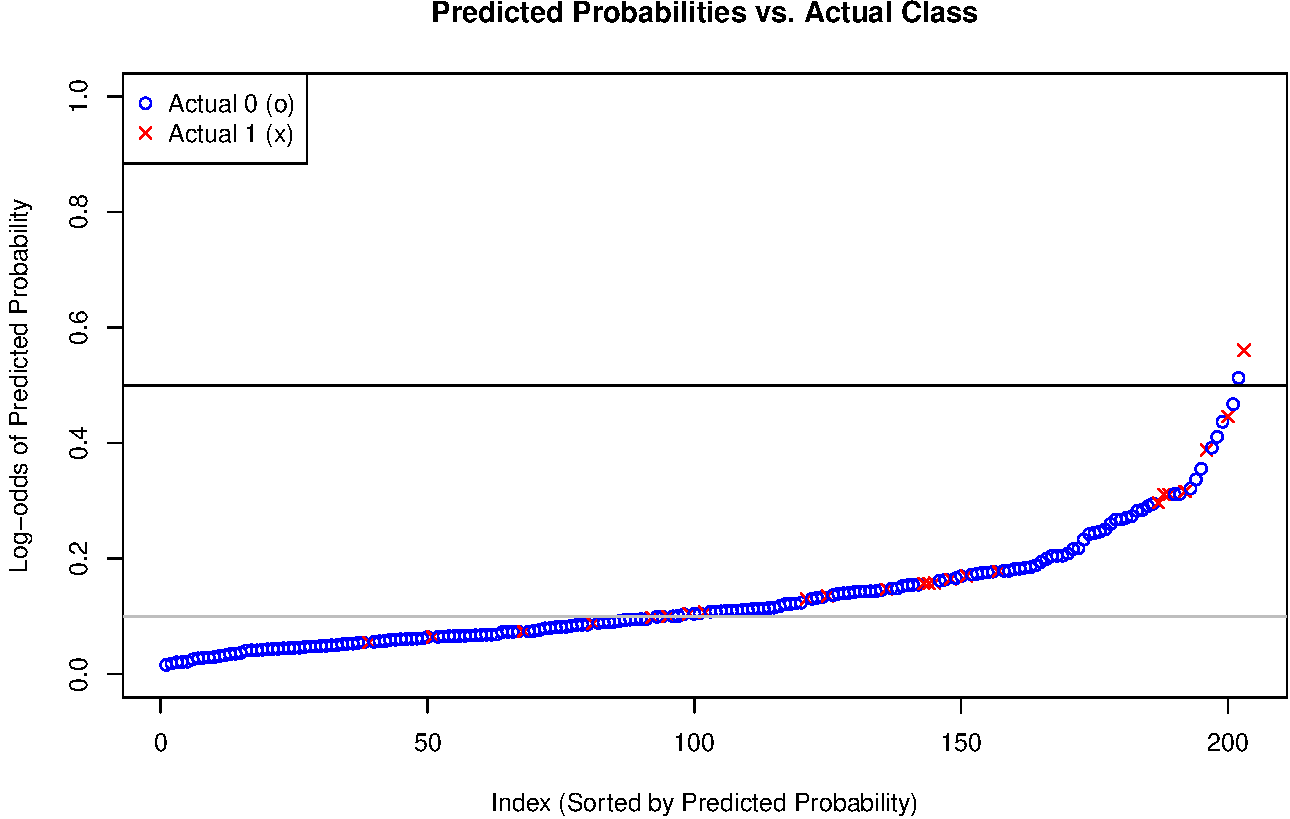
\includegraphics[keepaspectratio]{unit4-lr/logistic_files/figure-pdf/plot-sorted-probabilities-1.pdf}}

\textbf{ROC curve and Area Under the ROC (AUC)}

\begin{Shaded}
\begin{Highlighting}[]
\CommentTok{\# 4b. Area Under the Curve (AUC)}
\NormalTok{roc\_curve }\OtherTok{\textless{}{-}} \FunctionTok{roc}\NormalTok{(test\_data}\SpecialCharTok{$}\NormalTok{chd, pred\_probs, }\AttributeTok{quiet =} \ConstantTok{TRUE}\NormalTok{)}

\CommentTok{\# Plot the ROC curve}
\FunctionTok{plot}\NormalTok{(roc\_curve, }\AttributeTok{main =} \StringTok{"ROC Curve (Test Data)"}\NormalTok{, }\AttributeTok{print.auc =} \ConstantTok{TRUE}\NormalTok{)}
\end{Highlighting}
\end{Shaded}

\pandocbounded{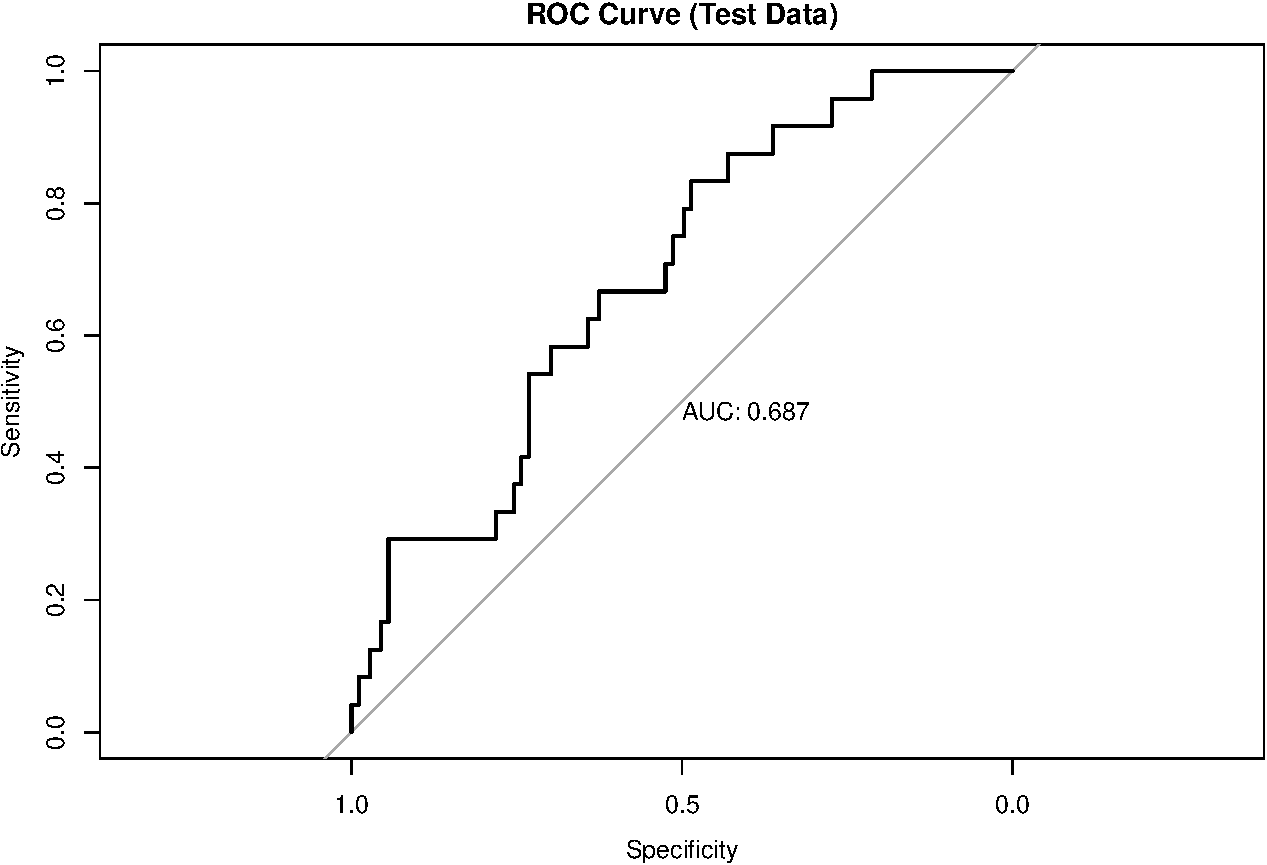
\includegraphics[keepaspectratio]{unit4-lr/logistic_files/figure-pdf/unnamed-chunk-9-1.pdf}}

\begin{Shaded}
\begin{Highlighting}[]
\NormalTok{auc\_value }\OtherTok{\textless{}{-}} \FunctionTok{auc}\NormalTok{(roc\_curve)}
\FunctionTok{cat}\NormalTok{(}\FunctionTok{paste}\NormalTok{(}\StringTok{"Area Under the Curve (AUC):"}\NormalTok{, }\FunctionTok{round}\NormalTok{(auc\_value, }\DecValTok{4}\NormalTok{), }\StringTok{"}\SpecialCharTok{\textbackslash{}n\textbackslash{}n}\StringTok{"}\NormalTok{))}
\end{Highlighting}
\end{Shaded}

\begin{verbatim}
Area Under the Curve (AUC): 0.6872 
\end{verbatim}

\textbf{PR curve and Area Under PR Curve (AUPR)}

\begin{Shaded}
\begin{Highlighting}[]
\CommentTok{\# Load the ROCR library}
\CommentTok{\# install.packages("ROCR") \# Uncomment to install if needed}
\FunctionTok{library}\NormalTok{(ROCR)}

\CommentTok{\# {-}{-}{-} 1. Create a \textquotesingle{}prediction\textquotesingle{} object {-}{-}{-}}
\CommentTok{\# \textquotesingle{}prediction\textquotesingle{} takes all predictions and all true labels}
\CommentTok{\# We use \textquotesingle{}pred\_probs\textquotesingle{} and \textquotesingle{}test\_data$chd\textquotesingle{} from the CHD data split}
\NormalTok{pred\_obj }\OtherTok{\textless{}{-}} \FunctionTok{prediction}\NormalTok{(pred\_probs, test\_data}\SpecialCharTok{$}\NormalTok{chd)}

\CommentTok{\# {-}{-}{-} 2. Create a \textquotesingle{}performance\textquotesingle{} object for PR {-}{-}{-}}
\CommentTok{\# "prec" is for precision, "rec" is for recall}
\NormalTok{perf\_pr }\OtherTok{\textless{}{-}} \FunctionTok{performance}\NormalTok{(pred\_obj, }\AttributeTok{measure =} \StringTok{"prec"}\NormalTok{, }\AttributeTok{x.measure =} \StringTok{"rec"}\NormalTok{)}

\CommentTok{\# {-}{-}{-} 3. Calculate Area Under the PR Curve (AUPR) {-}{-}{-}}
\NormalTok{perf\_auc }\OtherTok{\textless{}{-}} \FunctionTok{performance}\NormalTok{(pred\_obj, }\AttributeTok{measure =} \StringTok{"aucpr"}\NormalTok{) }\CommentTok{\# "aucpr" = Area Under PR Curve}
\NormalTok{aupr\_value }\OtherTok{\textless{}{-}}\NormalTok{ perf\_auc}\SpecialCharTok{@}\NormalTok{y.values[[}\DecValTok{1}\NormalTok{]]}
\FunctionTok{cat}\NormalTok{(}\FunctionTok{paste}\NormalTok{(}\StringTok{"Area Under PR Curve (AUPR):"}\NormalTok{, }\FunctionTok{round}\NormalTok{(aupr\_value, }\DecValTok{4}\NormalTok{), }\StringTok{"}\SpecialCharTok{\textbackslash{}n}\StringTok{"}\NormalTok{))}
\end{Highlighting}
\end{Shaded}

\begin{verbatim}
Area Under PR Curve (AUPR): 0.2826 
\end{verbatim}

\begin{Shaded}
\begin{Highlighting}[]
\CommentTok{\# {-}{-}{-} 4. Plot the performance object {-}{-}{-}}
\FunctionTok{plot}\NormalTok{(perf\_pr, }
     \AttributeTok{main =} \StringTok{"Precision{-}Recall Curve (Test Data)"}\NormalTok{, }
     \AttributeTok{xlim =} \FunctionTok{c}\NormalTok{(}\DecValTok{0}\NormalTok{, }\DecValTok{1}\NormalTok{), }
     \AttributeTok{ylim =} \FunctionTok{c}\NormalTok{(}\DecValTok{0}\NormalTok{, }\DecValTok{1}\NormalTok{),}
     \AttributeTok{col =} \StringTok{"black"}\NormalTok{)}

\CommentTok{\# {-}{-}{-} 5. Calculate and add the \textquotesingle{}no{-}skill\textquotesingle{} baseline {-}{-}{-}}
\NormalTok{baseline\_precision }\OtherTok{\textless{}{-}} \FunctionTok{sum}\NormalTok{(test\_data}\SpecialCharTok{$}\NormalTok{chd }\SpecialCharTok{==} \DecValTok{1}\NormalTok{) }\SpecialCharTok{/} \FunctionTok{length}\NormalTok{(test\_data}\SpecialCharTok{$}\NormalTok{chd)}
\FunctionTok{abline}\NormalTok{(}\AttributeTok{h =}\NormalTok{ baseline\_precision, }\AttributeTok{col =} \StringTok{"blue"}\NormalTok{, }\AttributeTok{lty =} \DecValTok{2}\NormalTok{)}

\CommentTok{\# {-}{-}{-} 6. Add a legend with AUPR {-}{-}{-}}
\FunctionTok{legend}\NormalTok{(}\StringTok{"bottomleft"}\NormalTok{, }
       \AttributeTok{legend =} \FunctionTok{c}\NormalTok{(}
           \FunctionTok{paste}\NormalTok{(}\StringTok{"Model (AUPR ="}\NormalTok{, }\FunctionTok{round}\NormalTok{(aupr\_value, }\DecValTok{4}\NormalTok{), }\StringTok{")"}\NormalTok{),  }\CommentTok{\# \textless{}{-}{-} MODIFIED LINE}
           \FunctionTok{paste}\NormalTok{(}\StringTok{"Baseline ("}\NormalTok{, }\FunctionTok{round}\NormalTok{(baseline\_precision, }\DecValTok{3}\NormalTok{), }\StringTok{")"}\NormalTok{)}
\NormalTok{       ), }
       \AttributeTok{col =} \FunctionTok{c}\NormalTok{(}\StringTok{"black"}\NormalTok{, }\StringTok{"blue"}\NormalTok{), }
       \AttributeTok{lty =} \FunctionTok{c}\NormalTok{(}\DecValTok{1}\NormalTok{, }\DecValTok{2}\NormalTok{), }
       \AttributeTok{bty =} \StringTok{"n"}\NormalTok{) }\CommentTok{\# bty="n" removes the box}
\end{Highlighting}
\end{Shaded}

\pandocbounded{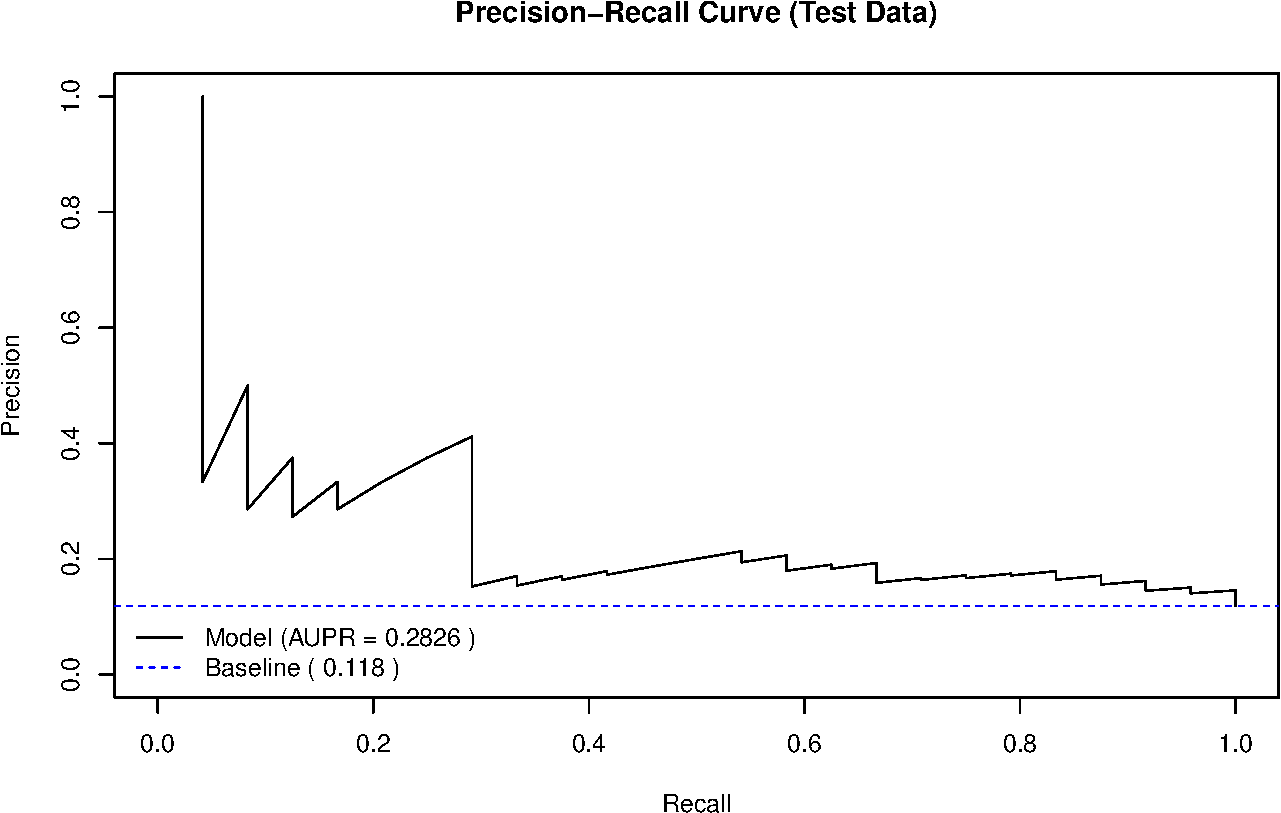
\includegraphics[keepaspectratio]{unit4-lr/logistic_files/figure-pdf/pr-curve-rocr-chd-1.pdf}}

\section{One-factor Design}\label{one-factor-design}

\section{Completely Randomized
Design}\label{completely-randomized-design}

\subsection{Plasma Etching Experiment}\label{plasma-etching-experiment}

This section analyzes data from a \textbf{Completely Randomized Design
(CRD)}. In a CRD, experimental units (in this case, the silicon wafers
being etched) are assigned to treatments (the RF Power levels)
completely at random. The primary goal is to determine if changing the
RF Power level has a statistically significant effect on the mean etch
rate.

\subsubsection{Data and Visualization}\label{data-and-visualization}

We begin by loading the data into a single, tidy \texttt{data.frame}.
The response variable, \texttt{rate}, contains all the etch rate
observations. The predictor variable, \texttt{power}, is a
\textbf{factor}, which is R's way of representing a categorical
variable. This tells R to treat the different power levels as distinct
groups.

\begin{Shaded}
\begin{Highlighting}[]
\CommentTok{\# Define the data vectors}
\NormalTok{rate }\OtherTok{\textless{}{-}} \FunctionTok{c}\NormalTok{(}\DecValTok{575}\NormalTok{, }\DecValTok{542}\NormalTok{, }\DecValTok{530}\NormalTok{, }\DecValTok{539}\NormalTok{, }\DecValTok{570}\NormalTok{, }\DecValTok{565}\NormalTok{, }\DecValTok{593}\NormalTok{, }\DecValTok{590}\NormalTok{, }\DecValTok{579}\NormalTok{, }\DecValTok{610}\NormalTok{,}
          \DecValTok{600}\NormalTok{, }\DecValTok{651}\NormalTok{, }\DecValTok{610}\NormalTok{, }\DecValTok{637}\NormalTok{, }\DecValTok{629}\NormalTok{, }\DecValTok{725}\NormalTok{, }\DecValTok{700}\NormalTok{, }\DecValTok{715}\NormalTok{, }\DecValTok{685}\NormalTok{, }\DecValTok{710}\NormalTok{)}
\NormalTok{power\_levels }\OtherTok{\textless{}{-}} \FunctionTok{c}\NormalTok{(}\DecValTok{160}\NormalTok{, }\DecValTok{180}\NormalTok{, }\DecValTok{200}\NormalTok{, }\DecValTok{220}\NormalTok{)}

\CommentTok{\# Create the data frame}
\NormalTok{etching\_df }\OtherTok{\textless{}{-}} \FunctionTok{data.frame}\NormalTok{(}
  \AttributeTok{rate =}\NormalTok{ rate,}
  \AttributeTok{power =} \FunctionTok{factor}\NormalTok{(}\FunctionTok{rep}\NormalTok{(power\_levels, }\AttributeTok{each =} \DecValTok{5}\NormalTok{))}
\NormalTok{)}

\CommentTok{\# Display the first few rows}
\NormalTok{etching\_df}
\end{Highlighting}
\end{Shaded}

\begin{verbatim}
   rate power
1   575   160
2   542   160
3   530   160
4   539   160
5   570   160
6   565   180
7   593   180
8   590   180
9   579   180
10  610   180
11  600   200
12  651   200
13  610   200
14  637   200
15  629   200
16  725   220
17  700   220
18  715   220
19  685   220
20  710   220
\end{verbatim}

\textbf{Grouped Boxplots}

\begin{Shaded}
\begin{Highlighting}[]
\FunctionTok{boxplot}\NormalTok{(rate}\SpecialCharTok{\textasciitilde{}}\NormalTok{power, }\AttributeTok{data=}\NormalTok{etching\_df)}
\end{Highlighting}
\end{Shaded}

\pandocbounded{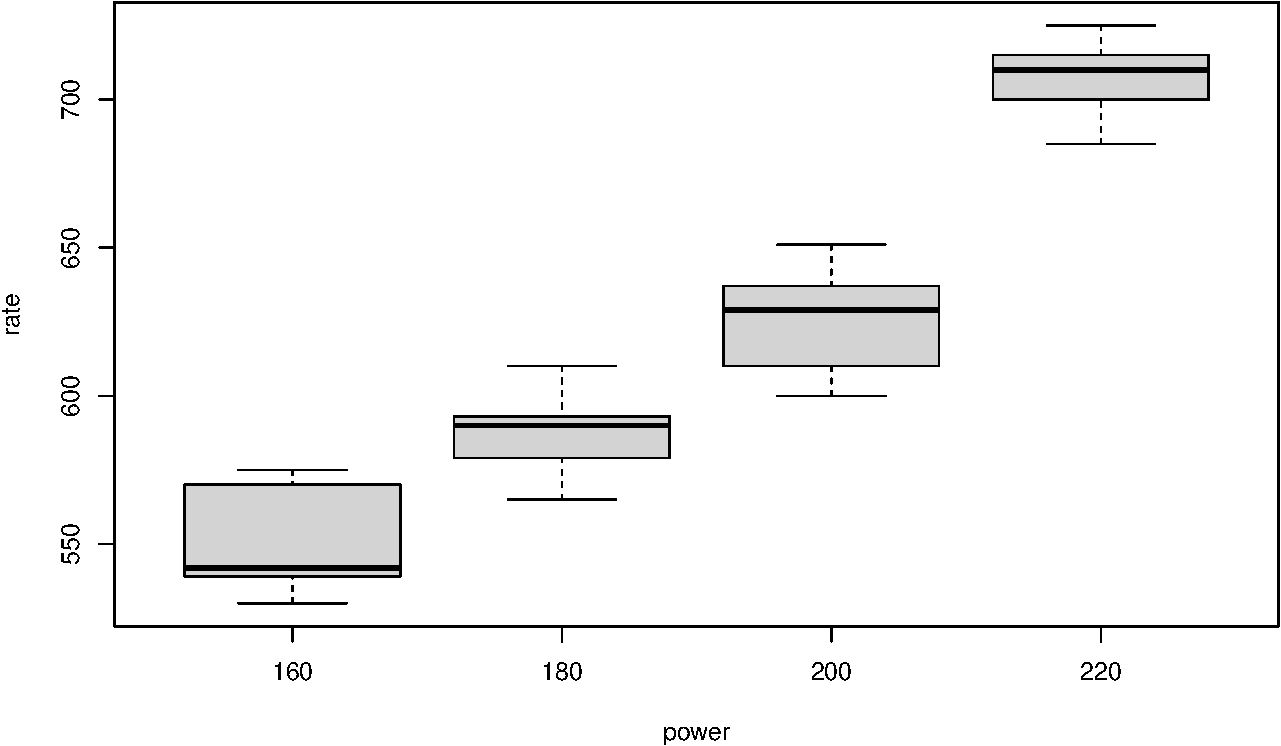
\includegraphics[keepaspectratio]{unit5-factor/crbd_files/figure-pdf/unnamed-chunk-1-1.pdf}}

\textbf{Using ggplot to visualize grouped data}

\begin{Shaded}
\begin{Highlighting}[]
\FunctionTok{library}\NormalTok{(ggplot2)}
\FunctionTok{library}\NormalTok{(dplyr) }\CommentTok{\# Using dplyr for easier data manipulation}

\CommentTok{\# Calculate group means and their start/end indices}
\NormalTok{mean\_rates }\OtherTok{\textless{}{-}}\NormalTok{ etching\_df }\SpecialCharTok{\%\textgreater{}\%}
  \FunctionTok{mutate}\NormalTok{(}\AttributeTok{obs\_index =} \FunctionTok{row\_number}\NormalTok{()) }\SpecialCharTok{\%\textgreater{}\%}
  \FunctionTok{group\_by}\NormalTok{(power) }\SpecialCharTok{\%\textgreater{}\%}
  \FunctionTok{summarise}\NormalTok{(}
    \AttributeTok{mean\_rate =} \FunctionTok{mean}\NormalTok{(rate),}
    \AttributeTok{x\_start =} \FunctionTok{min}\NormalTok{(obs\_index) }\SpecialCharTok{{-}} \FloatTok{0.5}\NormalTok{,}
    \AttributeTok{x\_end =} \FunctionTok{max}\NormalTok{(obs\_index) }\SpecialCharTok{+} \FloatTok{0.5}
\NormalTok{  )}

\FunctionTok{ggplot}\NormalTok{(etching\_df, }\FunctionTok{aes}\NormalTok{(}\AttributeTok{x =} \DecValTok{1}\SpecialCharTok{:}\FunctionTok{nrow}\NormalTok{(etching\_df), }\AttributeTok{y =}\NormalTok{ rate, }\AttributeTok{color =}\NormalTok{ power)) }\SpecialCharTok{+}
  \FunctionTok{geom\_point}\NormalTok{(}\AttributeTok{size =} \DecValTok{3}\NormalTok{, }\AttributeTok{alpha =} \FloatTok{0.7}\NormalTok{) }\SpecialCharTok{+} \CommentTok{\# Plot individual data points}
  \FunctionTok{geom\_segment}\NormalTok{(}
    \AttributeTok{data =}\NormalTok{ mean\_rates, }
    \FunctionTok{aes}\NormalTok{(}\AttributeTok{x =}\NormalTok{ x\_start, }\AttributeTok{xend =}\NormalTok{ x\_end, }\AttributeTok{y =}\NormalTok{ mean\_rate, }\AttributeTok{yend =}\NormalTok{ mean\_rate),}
    \AttributeTok{linetype =} \StringTok{"dashed"}\NormalTok{, }
    \AttributeTok{size =} \FloatTok{1.2}
\NormalTok{  ) }\SpecialCharTok{+} \CommentTok{\# Add line segments for group means}
  \FunctionTok{labs}\NormalTok{(}
    \AttributeTok{title =} \StringTok{"Etch Rate Observations by RF Power Level"}\NormalTok{,}
    \AttributeTok{x =} \StringTok{"Observation Index"}\NormalTok{,}
    \AttributeTok{y =} \StringTok{"Etch Rate"}\NormalTok{,}
    \AttributeTok{color =} \StringTok{"RF Power (W)"}
\NormalTok{  ) }\SpecialCharTok{+}
  \FunctionTok{scale\_color\_brewer}\NormalTok{(}\AttributeTok{palette =} \StringTok{"Set1"}\NormalTok{) }\SpecialCharTok{+}
  \FunctionTok{theme\_minimal}\NormalTok{() }\SpecialCharTok{+}
  \FunctionTok{theme}\NormalTok{(}\AttributeTok{plot.title =} \FunctionTok{element\_text}\NormalTok{(}\AttributeTok{hjust =} \FloatTok{0.5}\NormalTok{))}
\end{Highlighting}
\end{Shaded}

\begin{figure}[H]

{\centering \pandocbounded{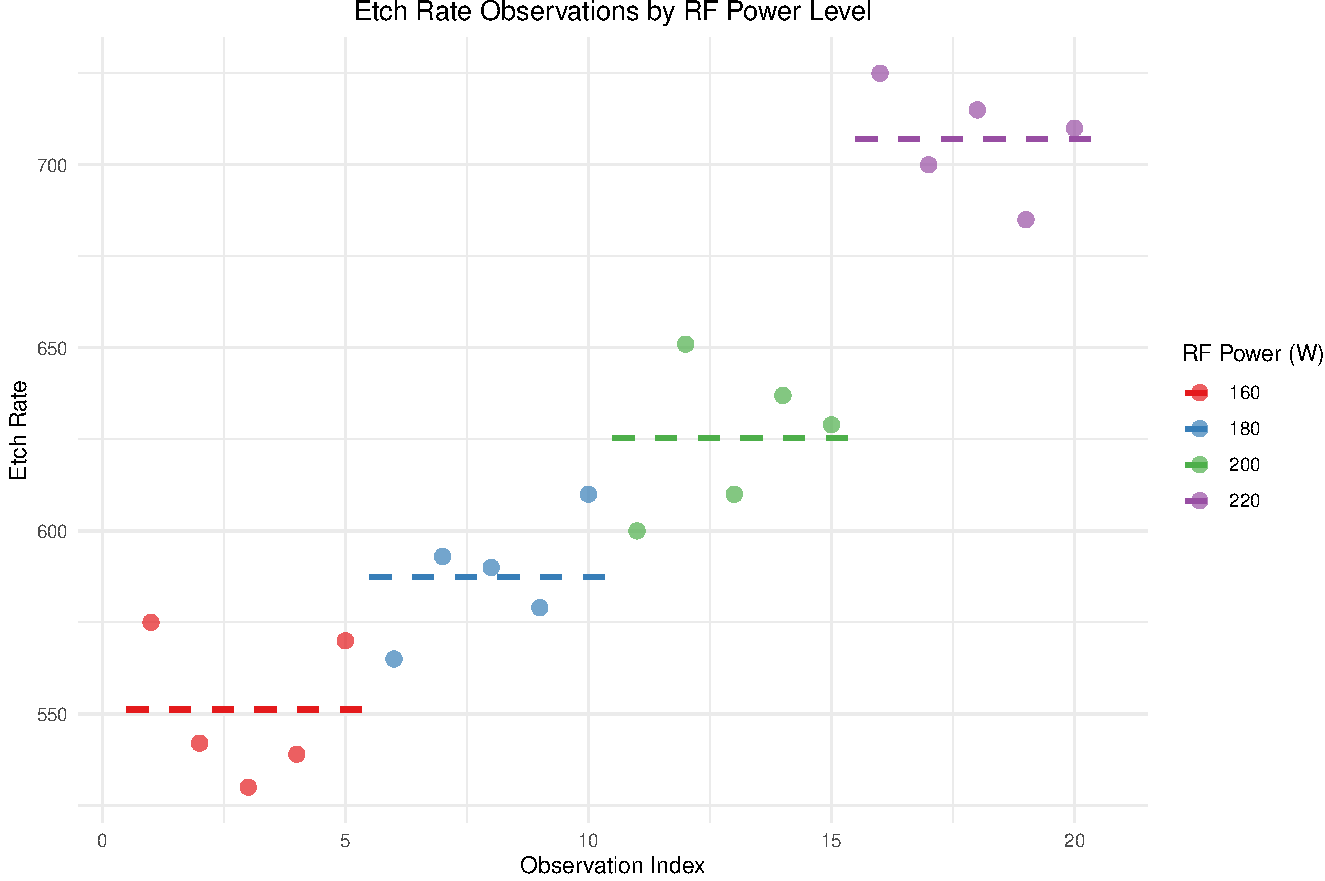
\includegraphics[keepaspectratio]{unit5-factor/crbd_files/figure-pdf/index-plot-rate-power-segments-1.pdf}}

}

\caption{Index Plot of Etch Rate with Group-Specific Mean Lines}

\end{figure}%

\subsubsection{Model Fitting with Sum-to-Zero
Constraint}\label{model-fitting-with-sum-to-zero-constraint}

We fit a linear model using the \texttt{lm()} function to perform an
\textbf{Analysis of Variance (ANOVA)}. The model is specified as
\texttt{rate\ \textasciitilde{}\ power}, and we now include the
\texttt{data\ =\ etching\_df} argument.

To get interpretable estimates for the treatment effects (\(\tau_i\)),
we use a \textbf{sum-to-zero constraint} (\texttt{contr.sum}), which
forces the sum of the treatment effects to be zero
(\(\sum \tau_i = 0\)).

\begin{Shaded}
\begin{Highlighting}[]
\NormalTok{fit }\OtherTok{\textless{}{-}} \FunctionTok{lm}\NormalTok{(rate }\SpecialCharTok{\textasciitilde{}}\NormalTok{ power, }\AttributeTok{data =}\NormalTok{ etching\_df, }\AttributeTok{contrasts =} \FunctionTok{list}\NormalTok{(}\AttributeTok{power =}\NormalTok{ contr.sum))}
\FunctionTok{cat}\NormalTok{ (}\StringTok{"Model Matrix:}\SpecialCharTok{\textbackslash{}n}\StringTok{"}\NormalTok{)}
\end{Highlighting}
\end{Shaded}

\begin{verbatim}
Model Matrix:
\end{verbatim}

\begin{Shaded}
\begin{Highlighting}[]
\FunctionTok{model.matrix}\NormalTok{(fit)}
\end{Highlighting}
\end{Shaded}

\begin{verbatim}
   (Intercept) power1 power2 power3
1            1      1      0      0
2            1      1      0      0
3            1      1      0      0
4            1      1      0      0
5            1      1      0      0
6            1      0      1      0
7            1      0      1      0
8            1      0      1      0
9            1      0      1      0
10           1      0      1      0
11           1      0      0      1
12           1      0      0      1
13           1      0      0      1
14           1      0      0      1
15           1      0      0      1
16           1     -1     -1     -1
17           1     -1     -1     -1
18           1     -1     -1     -1
19           1     -1     -1     -1
20           1     -1     -1     -1
attr(,"assign")
[1] 0 1 1 1
attr(,"contrasts")
attr(,"contrasts")$power
    [,1] [,2] [,3]
160    1    0    0
180    0    1    0
200    0    0    1
220   -1   -1   -1
\end{verbatim}

\begin{Shaded}
\begin{Highlighting}[]
\NormalTok{summary.fit }\OtherTok{\textless{}{-}} \FunctionTok{summary}\NormalTok{(fit)}
\FunctionTok{cat}\NormalTok{ (}\StringTok{"Summary of lm fitting results:}\SpecialCharTok{\textbackslash{}n}\StringTok{"}\NormalTok{)}
\end{Highlighting}
\end{Shaded}

\begin{verbatim}
Summary of lm fitting results:
\end{verbatim}

\begin{Shaded}
\begin{Highlighting}[]
\NormalTok{summary.fit}
\end{Highlighting}
\end{Shaded}

\begin{verbatim}

Call:
lm(formula = rate ~ power, data = etching_df, contrasts = list(power = contr.sum))

Residuals:
   Min     1Q Median     3Q    Max 
 -25.4  -13.0    2.8   13.2   25.6 

Coefficients:
            Estimate Std. Error t value Pr(>|t|)    
(Intercept)  617.750      4.085 151.234  < 2e-16 ***
power1       -66.550      7.075  -9.406 6.39e-08 ***
power2       -30.350      7.075  -4.290 0.000563 ***
power3         7.650      7.075   1.081 0.295602    
---
Signif. codes:  0 '***' 0.001 '**' 0.01 '*' 0.05 '.' 0.1 ' ' 1

Residual standard error: 18.27 on 16 degrees of freedom
Multiple R-squared:  0.9261,    Adjusted R-squared:  0.9122 
F-statistic:  66.8 on 3 and 16 DF,  p-value: 2.883e-09
\end{verbatim}

\subsubsection{Point Estimation of
Parameters}\label{point-estimation-of-parameters}

The output of the model provides estimates for the overall mean
(\(\hat{\mu}\)) and the treatment effects for the first k-1 levels
(\(\hat{\tau}_1, \hat{\tau}_2, \hat{\tau}_3\)).

\begin{itemize}
\tightlist
\item
  \(\hat{\mu}\) (the Intercept) is the estimate of the grand mean etch
  rate across all power levels.
\item
  \(\hat{\tau}_i\) is the estimated effect of the i-th power level,
  representing how much that level's mean deviates from the grand mean.
\end{itemize}

Using the sum-to-zero constraint, we can manually calculate the effect
for the final level, \(\hat{\tau}_4\).

\begin{Shaded}
\begin{Highlighting}[]
\CommentTok{\# Extract coefficients}
\NormalTok{est }\OtherTok{\textless{}{-}} \FunctionTok{coef}\NormalTok{(fit)}
\NormalTok{tau4.hat }\OtherTok{\textless{}{-}} \SpecialCharTok{{-}}\FunctionTok{sum}\NormalTok{(est[}\SpecialCharTok{{-}}\DecValTok{1}\NormalTok{])}
\NormalTok{taui.hat }\OtherTok{\textless{}{-}} \FunctionTok{c}\NormalTok{(est[}\SpecialCharTok{{-}}\DecValTok{1}\NormalTok{], tau4.hat)}
\FunctionTok{print}\NormalTok{(}\StringTok{"Estimated Treatment Effects (tau\_i):"}\NormalTok{)}
\end{Highlighting}
\end{Shaded}

\begin{verbatim}
[1] "Estimated Treatment Effects (tau_i):"
\end{verbatim}

\begin{Shaded}
\begin{Highlighting}[]
\FunctionTok{print}\NormalTok{(taui.hat)}
\end{Highlighting}
\end{Shaded}

\begin{verbatim}
power1 power2 power3        
-66.55 -30.35   7.65  89.25 
\end{verbatim}

\begin{Shaded}
\begin{Highlighting}[]
\CommentTok{\# Estimates of treatment means (mu\_i)}
\NormalTok{mu.hat }\OtherTok{\textless{}{-}}\NormalTok{ est[}\DecValTok{1}\NormalTok{]}
\NormalTok{mui.hat }\OtherTok{\textless{}{-}}\NormalTok{ mu.hat }\SpecialCharTok{+}\NormalTok{ taui.hat}
\FunctionTok{print}\NormalTok{(}\StringTok{"Estimated Treatment Means (mu\_i):"}\NormalTok{)}
\end{Highlighting}
\end{Shaded}

\begin{verbatim}
[1] "Estimated Treatment Means (mu_i):"
\end{verbatim}

\begin{Shaded}
\begin{Highlighting}[]
\FunctionTok{print}\NormalTok{(mui.hat)}
\end{Highlighting}
\end{Shaded}

\begin{verbatim}
power1 power2 power3        
 551.2  587.4  625.4  707.0 
\end{verbatim}

\subsubsection{ANOVA Table}\label{anova-table}

The ANOVA table partitions the total variation into variation
\textbf{between} treatment groups (\texttt{power}) and variation
\textbf{within} treatment groups (random error). The \textbf{p-value}
(Pr(\textgreater F)) indicates if the treatment has a significant
effect.

\begin{Shaded}
\begin{Highlighting}[]
\FunctionTok{anova}\NormalTok{(fit)}
\end{Highlighting}
\end{Shaded}

\begin{verbatim}
Analysis of Variance Table

Response: rate
          Df Sum Sq Mean Sq F value    Pr(>F)    
power      3  66871 22290.2  66.797 2.883e-09 ***
Residuals 16   5339   333.7                      
---
Signif. codes:  0 '***' 0.001 '**' 0.01 '*' 0.05 '.' 0.1 ' ' 1
\end{verbatim}

\subsubsection{95\% Confidence Intervals for Treatment
Means}\label{confidence-intervals-for-treatment-means}

A \textbf{confidence interval} provides a range of plausible values for
the true mean etch rate at each power level.

\begin{Shaded}
\begin{Highlighting}[]
\CommentTok{\# Number of replicates}
\NormalTok{n }\OtherTok{\textless{}{-}} \DecValTok{5} 
\CommentTok{\# Extract sqrt(MSE) and error df}
\NormalTok{sqrt.MSE }\OtherTok{\textless{}{-}}\NormalTok{ summary.fit}\SpecialCharTok{$}\NormalTok{sigma}
\NormalTok{DF }\OtherTok{\textless{}{-}}\NormalTok{ fit}\SpecialCharTok{$}\NormalTok{df.residual}
\CommentTok{\# Find t{-}value}
\NormalTok{t.value }\OtherTok{\textless{}{-}} \FunctionTok{qt}\NormalTok{(}\FloatTok{0.975}\NormalTok{, DF)}
\CommentTok{\# Calculate CIs}
\NormalTok{CI.lower }\OtherTok{\textless{}{-}}\NormalTok{ mui.hat }\SpecialCharTok{{-}}\NormalTok{ t.value }\SpecialCharTok{*}\NormalTok{ sqrt.MSE }\SpecialCharTok{/} \FunctionTok{sqrt}\NormalTok{(n)}
\NormalTok{CI.upper }\OtherTok{\textless{}{-}}\NormalTok{ mui.hat }\SpecialCharTok{+}\NormalTok{ t.value }\SpecialCharTok{*}\NormalTok{ sqrt.MSE }\SpecialCharTok{/} \FunctionTok{sqrt}\NormalTok{(n)}

\CommentTok{\# Display CIs}
\FunctionTok{data.frame}\NormalTok{(}\AttributeTok{Power\_Level =}\NormalTok{ power\_levels, }\AttributeTok{Mean =}\NormalTok{ mui.hat, }\AttributeTok{Lower\_CI =}\NormalTok{ CI.lower, }\AttributeTok{Upper\_CI =}\NormalTok{ CI.upper)}
\end{Highlighting}
\end{Shaded}

\begin{verbatim}
       Power_Level  Mean Lower_CI Upper_CI
power1         160 551.2 533.8815 568.5185
power2         180 587.4 570.0815 604.7185
power3         200 625.4 608.0815 642.7185
               220 707.0 689.6815 724.3185
\end{verbatim}

\textbf{Alternatively, one can use a model without intercept}

\begin{Shaded}
\begin{Highlighting}[]
\NormalTok{fit\_nointercpt }\OtherTok{\textless{}{-}} \FunctionTok{lm}\NormalTok{(rate }\SpecialCharTok{\textasciitilde{}} \DecValTok{0}\SpecialCharTok{+}\NormalTok{power, }\AttributeTok{data =}\NormalTok{ etching\_df)}
\FunctionTok{summary}\NormalTok{(fit\_nointercpt)}
\end{Highlighting}
\end{Shaded}

\begin{verbatim}

Call:
lm(formula = rate ~ 0 + power, data = etching_df)

Residuals:
   Min     1Q Median     3Q    Max 
 -25.4  -13.0    2.8   13.2   25.6 

Coefficients:
         Estimate Std. Error t value Pr(>|t|)    
power160  551.200      8.169   67.47   <2e-16 ***
power180  587.400      8.169   71.90   <2e-16 ***
power200  625.400      8.169   76.55   <2e-16 ***
power220  707.000      8.169   86.54   <2e-16 ***
---
Signif. codes:  0 '***' 0.001 '**' 0.01 '*' 0.05 '.' 0.1 ' ' 1

Residual standard error: 18.27 on 16 degrees of freedom
Multiple R-squared:  0.9993,    Adjusted R-squared:  0.9991 
F-statistic:  5768 on 4 and 16 DF,  p-value: < 2.2e-16
\end{verbatim}

\begin{Shaded}
\begin{Highlighting}[]
\FunctionTok{confint}\NormalTok{(fit\_nointercpt)}
\end{Highlighting}
\end{Shaded}

\begin{verbatim}
            2.5 %   97.5 %
power160 533.8815 568.5185
power180 570.0815 604.7185
power200 608.0815 642.7185
power220 689.6815 724.3185
\end{verbatim}

\subsubsection{Comparison with Default ``Treatment''
Contrast}\label{comparison-with-default-treatment-contrast}

Fitting the model without specifying contrasts uses R's default
(``treatment'' contrast), which sets \(\tau_1 = 0\). The fundamental
results (ANOVA, treatment means) remain unchanged.

\begin{Shaded}
\begin{Highlighting}[]
\NormalTok{fit1 }\OtherTok{\textless{}{-}} \FunctionTok{lm}\NormalTok{(rate }\SpecialCharTok{\textasciitilde{}}\NormalTok{ power, }\AttributeTok{data =}\NormalTok{ etching\_df)}
\FunctionTok{summary}\NormalTok{(fit1)}
\end{Highlighting}
\end{Shaded}

\begin{verbatim}

Call:
lm(formula = rate ~ power, data = etching_df)

Residuals:
   Min     1Q Median     3Q    Max 
 -25.4  -13.0    2.8   13.2   25.6 

Coefficients:
            Estimate Std. Error t value Pr(>|t|)    
(Intercept)  551.200      8.169  67.471  < 2e-16 ***
power180      36.200     11.553   3.133  0.00642 ** 
power200      74.200     11.553   6.422 8.44e-06 ***
power220     155.800     11.553  13.485 3.73e-10 ***
---
Signif. codes:  0 '***' 0.001 '**' 0.01 '*' 0.05 '.' 0.1 ' ' 1

Residual standard error: 18.27 on 16 degrees of freedom
Multiple R-squared:  0.9261,    Adjusted R-squared:  0.9122 
F-statistic:  66.8 on 3 and 16 DF,  p-value: 2.883e-09
\end{verbatim}

\subsubsection{Pairwise Comparisons}\label{pairwise-comparisons}

Since our ANOVA result was significant, we perform \textbf{post-hoc
tests} to determine exactly which pairs of power levels have different
means.

\paragraph{Tukey's HSD Test}\label{tukeys-hsd-test}

\textbf{Tukey's Honest Significant Difference (HSD)} controls the
\textbf{family-wise error rate}, adjusting p-values to account for
multiple comparisons.

\begin{Shaded}
\begin{Highlighting}[]
\NormalTok{fit.aov }\OtherTok{\textless{}{-}} \FunctionTok{aov}\NormalTok{(rate }\SpecialCharTok{\textasciitilde{}}\NormalTok{ power, }\AttributeTok{data =}\NormalTok{ etching\_df)}
\FunctionTok{TukeyHSD}\NormalTok{(fit.aov)}
\end{Highlighting}
\end{Shaded}

\begin{verbatim}
  Tukey multiple comparisons of means
    95% family-wise confidence level

Fit: aov(formula = rate ~ power, data = etching_df)

$power
         diff        lwr       upr     p adj
180-160  36.2   3.145624  69.25438 0.0294279
200-160  74.2  41.145624 107.25438 0.0000455
220-160 155.8 122.745624 188.85438 0.0000000
200-180  38.0   4.945624  71.05438 0.0215995
220-180 119.6  86.545624 152.65438 0.0000001
220-200  81.6  48.545624 114.65438 0.0000146
\end{verbatim}

\paragraph{Fisher's LSD Test}\label{fishers-lsd-test}

The \textbf{Fisher's Least Significant Difference (LSD)} test does not
control the family-wise error rate but is more powerful.

\begin{Shaded}
\begin{Highlighting}[]
\FunctionTok{with}\NormalTok{(etching\_df, }\FunctionTok{pairwise.t.test}\NormalTok{(rate, power, }\AttributeTok{p.adj =} \StringTok{"none"}\NormalTok{))}
\end{Highlighting}
\end{Shaded}

\begin{verbatim}

    Pairwise comparisons using t tests with pooled SD 

data:  rate and power 

    160     180     200    
180 0.0064  -       -      
200 8.4e-06 0.0046  -      
220 3.7e-10 1.7e-08 2.7e-06

P value adjustment method: none 
\end{verbatim}

\subsubsection{Checking Model
Assumptions}\label{checking-model-assumptions}

The validity of our ANOVA results depends on three key assumptions about
the model's residuals. We use diagnostic plots to check them.

\begin{Shaded}
\begin{Highlighting}[]
\NormalTok{r }\OtherTok{\textless{}{-}} \FunctionTok{rstudent}\NormalTok{(fit)}
\NormalTok{fitted }\OtherTok{\textless{}{-}} \FunctionTok{fitted.values}\NormalTok{(fit)}
\end{Highlighting}
\end{Shaded}

\paragraph{Normality of Residuals}\label{normality-of-residuals}

A \textbf{Normal Q-Q plot} is used to check if the residuals are
normally distributed. The points should fall closely along the straight
diagonal line.

\begin{Shaded}
\begin{Highlighting}[]
\FunctionTok{qqnorm}\NormalTok{(r)}
\FunctionTok{qqline}\NormalTok{(r)}
\end{Highlighting}
\end{Shaded}

\begin{figure}[H]

{\centering \pandocbounded{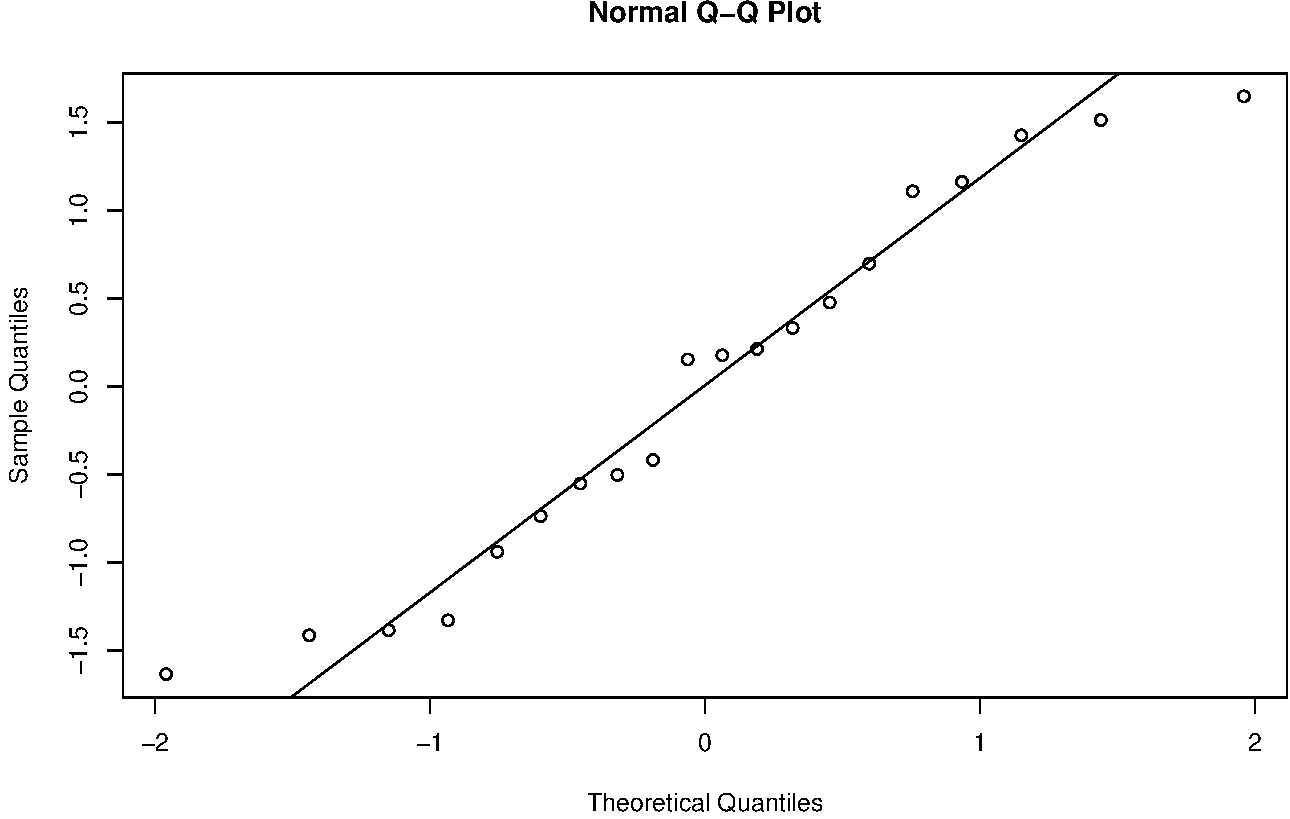
\includegraphics[keepaspectratio]{unit5-factor/crbd_files/figure-pdf/qq-plot-1.pdf}}

}

\caption{Normal Q-Q plot of standardized residuals.}

\end{figure}%

\paragraph{Independence of Residuals}\label{independence-of-residuals}

A plot of \textbf{residuals versus run order} helps check for
independence. We look for random scatter around the zero line.

\begin{Shaded}
\begin{Highlighting}[]
\FunctionTok{plot}\NormalTok{(r, }\AttributeTok{ylab =} \StringTok{"Standardized residuals"}\NormalTok{, }\AttributeTok{xlab =} \StringTok{"Run order"}\NormalTok{,}
     \AttributeTok{main =} \StringTok{"Plot of residuals vs. run order"}\NormalTok{)}
\FunctionTok{abline}\NormalTok{(}\AttributeTok{h =} \DecValTok{0}\NormalTok{)}
\end{Highlighting}
\end{Shaded}

\begin{figure}[H]

{\centering \pandocbounded{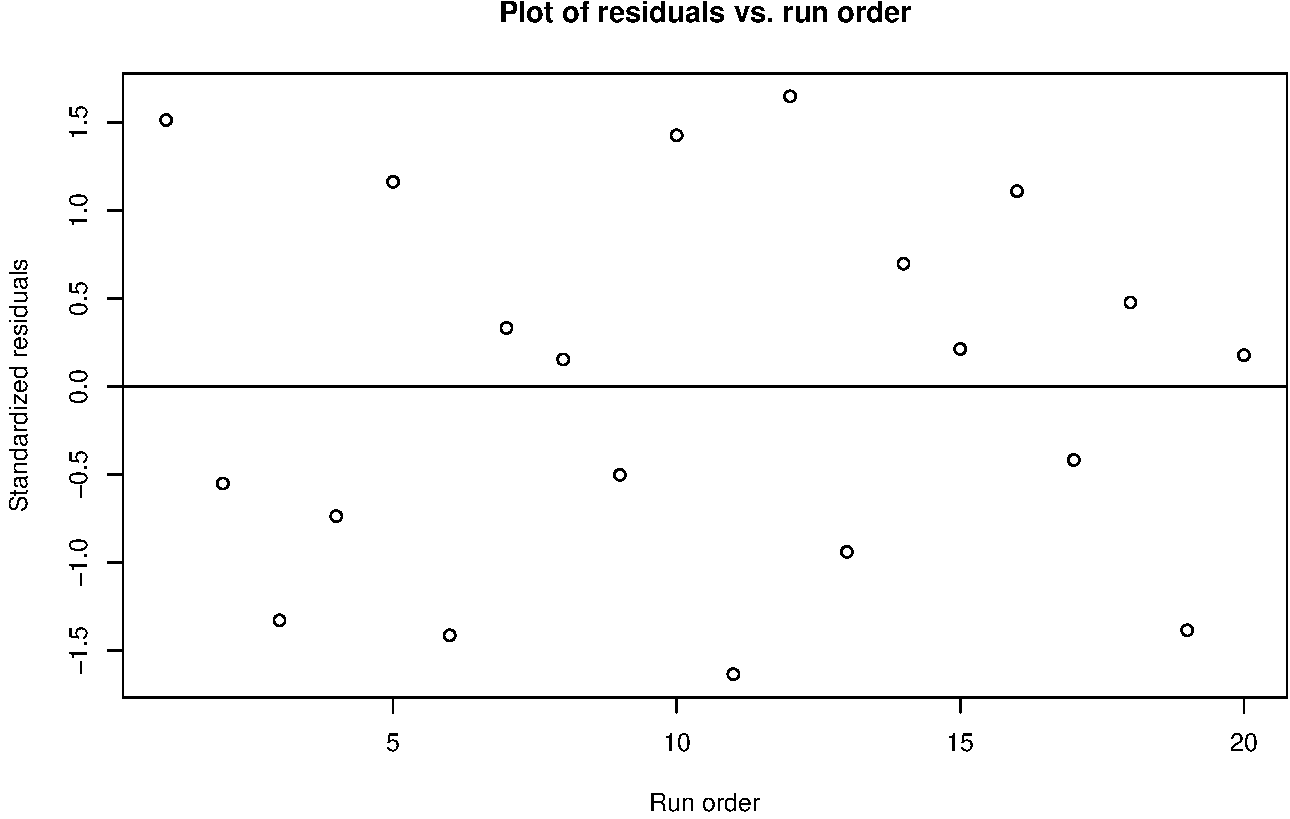
\includegraphics[keepaspectratio]{unit5-factor/crbd_files/figure-pdf/residuals-vs-order-1.pdf}}

}

\caption{Standardized residuals vs.~run order.}

\end{figure}%

\paragraph{Constant Variance
(Homoscedasticity)}\label{constant-variance-homoscedasticity}

A plot of \textbf{residuals versus fitted values} helps check for
constant variance. The spread of residuals should be roughly constant
across all fitted values.

\begin{Shaded}
\begin{Highlighting}[]
\FunctionTok{plot}\NormalTok{(fitted, r, }\AttributeTok{ylab =} \StringTok{"Standardized residuals"}\NormalTok{, }
     \AttributeTok{xlab =} \StringTok{"Fitted values"}\NormalTok{, }\AttributeTok{main =} \StringTok{"Plot of residuals vs. fitted values"}\NormalTok{)}
\FunctionTok{abline}\NormalTok{(}\AttributeTok{h =} \DecValTok{0}\NormalTok{)}
\end{Highlighting}
\end{Shaded}

\begin{figure}[H]

{\centering \pandocbounded{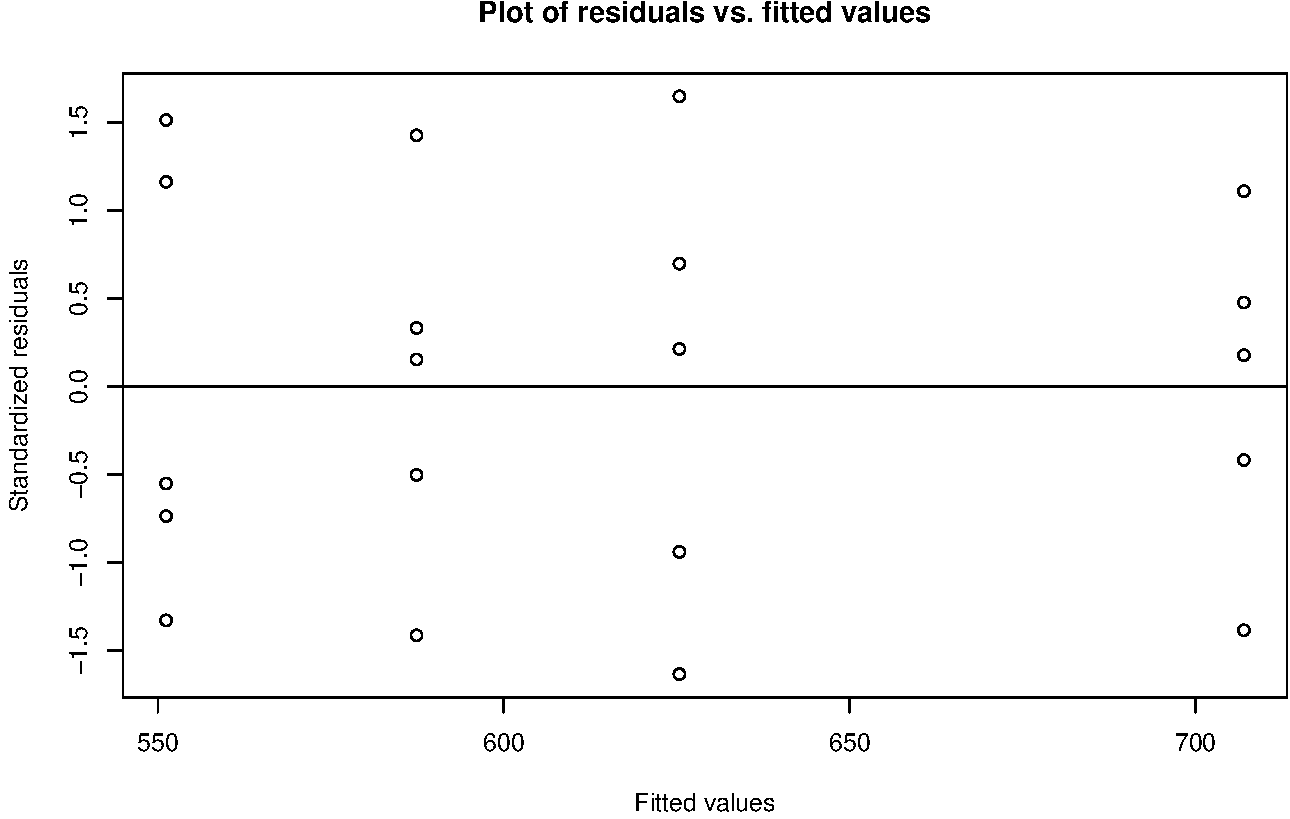
\includegraphics[keepaspectratio]{unit5-factor/crbd_files/figure-pdf/residuals-vs-fitted-1.pdf}}

}

\caption{Standardized residuals vs.~fitted values.}

\end{figure}%

\section{Unbalanced Designs with nequal Sample
Sizes}\label{unbalanced-designs-with-nequal-sample-sizes}

The ANOVA framework also handles \textbf{unbalanced designs}. We again
start by creating a data frame.

\begin{Shaded}
\begin{Highlighting}[]
\CommentTok{\# Create the data frame}
\NormalTok{bricks\_df }\OtherTok{\textless{}{-}} \FunctionTok{data.frame}\NormalTok{(}
  \AttributeTok{density =} \FunctionTok{c}\NormalTok{(}\FloatTok{21.8}\NormalTok{, }\FloatTok{21.9}\NormalTok{, }\FloatTok{21.7}\NormalTok{, }\FloatTok{21.6}\NormalTok{, }\FloatTok{21.7}\NormalTok{,}
              \FloatTok{21.7}\NormalTok{, }\FloatTok{21.4}\NormalTok{, }\FloatTok{21.5}\NormalTok{, }\FloatTok{21.4}\NormalTok{,}
              \FloatTok{21.9}\NormalTok{, }\FloatTok{21.8}\NormalTok{, }\FloatTok{21.8}\NormalTok{, }\FloatTok{21.6}\NormalTok{, }\FloatTok{21.5}\NormalTok{,}
              \FloatTok{21.9}\NormalTok{, }\FloatTok{21.7}\NormalTok{, }\FloatTok{21.8}\NormalTok{, }\FloatTok{21.4}\NormalTok{),}
  \AttributeTok{temperature =} \FunctionTok{factor}\NormalTok{(}\FunctionTok{c}\NormalTok{(}\FunctionTok{rep}\NormalTok{(}\DecValTok{100}\NormalTok{, }\DecValTok{5}\NormalTok{), }\FunctionTok{rep}\NormalTok{(}\DecValTok{125}\NormalTok{, }\DecValTok{4}\NormalTok{), }\FunctionTok{rep}\NormalTok{(}\DecValTok{150}\NormalTok{, }\DecValTok{5}\NormalTok{), }\FunctionTok{rep}\NormalTok{(}\DecValTok{175}\NormalTok{, }\DecValTok{4}\NormalTok{)))}
\NormalTok{)}

\NormalTok{bricks\_df}
\end{Highlighting}
\end{Shaded}

\begin{verbatim}
   density temperature
1     21.8         100
2     21.9         100
3     21.7         100
4     21.6         100
5     21.7         100
6     21.7         125
7     21.4         125
8     21.5         125
9     21.4         125
10    21.9         150
11    21.8         150
12    21.8         150
13    21.6         150
14    21.5         150
15    21.9         175
16    21.7         175
17    21.8         175
18    21.4         175
\end{verbatim}

\begin{Shaded}
\begin{Highlighting}[]
\CommentTok{\# Fit the model and get the ANOVA table}
\NormalTok{fit2 }\OtherTok{\textless{}{-}} \FunctionTok{lm}\NormalTok{(density }\SpecialCharTok{\textasciitilde{}}\NormalTok{ temperature, }\AttributeTok{data =}\NormalTok{ bricks\_df)}
\FunctionTok{summary}\NormalTok{(fit2)}
\end{Highlighting}
\end{Shaded}

\begin{verbatim}

Call:
lm(formula = density ~ temperature, data = bricks_df)

Residuals:
   Min     1Q Median     3Q    Max 
-0.300 -0.100  0.000  0.095  0.200 

Coefficients:
               Estimate Std. Error t value Pr(>|t|)    
(Intercept)    21.74000    0.07171 303.150   <2e-16 ***
temperature125 -0.24000    0.10757  -2.231   0.0425 *  
temperature150 -0.02000    0.10142  -0.197   0.8465    
temperature175 -0.04000    0.10757  -0.372   0.7156    
---
Signif. codes:  0 '***' 0.001 '**' 0.01 '*' 0.05 '.' 0.1 ' ' 1

Residual standard error: 0.1604 on 14 degrees of freedom
Multiple R-squared:  0.3025,    Adjusted R-squared:  0.153 
F-statistic: 2.024 on 3 and 14 DF,  p-value: 0.1569
\end{verbatim}

\begin{Shaded}
\begin{Highlighting}[]
\FunctionTok{anova}\NormalTok{(fit2)}
\end{Highlighting}
\end{Shaded}

\begin{verbatim}
Analysis of Variance Table

Response: density
            Df  Sum Sq  Mean Sq F value Pr(>F)
temperature  3 0.15611 0.052037  2.0237 0.1569
Residuals   14 0.36000 0.025714               
\end{verbatim}

In this case, the large p-value (0.133) indicates that there is no
statistically significant evidence that firing temperature affects brick
density.

\section{Randomized Complete Block
Design}\label{randomized-complete-block-design}

\subsection{Vascular Graft Experiment}\label{vascular-graft-experiment}

This section analyzes a \textbf{Randomized Complete Block Design
(RCBD)}, used to control for a known source of variability (here,
``batches of resin,'' treated as \textbf{blocks}).

\subsubsection{Data and Visulization}\label{data-and-visulization}

We structure the data in a \texttt{data.frame} to identify the response,
treatment (\texttt{pressure}), and block (\texttt{batch}) for each
observation.

\begin{Shaded}
\begin{Highlighting}[]
\CommentTok{\# Define data vectors}
\NormalTok{strength }\OtherTok{\textless{}{-}} \FunctionTok{c}\NormalTok{(}\FloatTok{90.3}\NormalTok{, }\FloatTok{89.2}\NormalTok{, }\FloatTok{98.2}\NormalTok{, }\FloatTok{93.9}\NormalTok{, }\FloatTok{87.4}\NormalTok{, }\FloatTok{97.9}\NormalTok{,}
              \FloatTok{92.5}\NormalTok{, }\FloatTok{89.5}\NormalTok{, }\FloatTok{90.6}\NormalTok{, }\FloatTok{94.7}\NormalTok{, }\FloatTok{87.0}\NormalTok{, }\FloatTok{95.8}\NormalTok{,}
              \FloatTok{85.5}\NormalTok{, }\FloatTok{90.8}\NormalTok{, }\FloatTok{89.6}\NormalTok{, }\FloatTok{86.2}\NormalTok{, }\FloatTok{88.0}\NormalTok{, }\FloatTok{93.4}\NormalTok{,}
              \FloatTok{82.5}\NormalTok{, }\FloatTok{89.5}\NormalTok{, }\FloatTok{85.6}\NormalTok{, }\FloatTok{87.4}\NormalTok{, }\FloatTok{78.9}\NormalTok{, }\FloatTok{90.7}\NormalTok{)}
\NormalTok{pressure\_levels }\OtherTok{\textless{}{-}} \FunctionTok{rep}\NormalTok{(}\FunctionTok{c}\NormalTok{(}\DecValTok{8500}\NormalTok{, }\DecValTok{8700}\NormalTok{, }\DecValTok{8900}\NormalTok{, }\DecValTok{9100}\NormalTok{), }\AttributeTok{each =} \DecValTok{6}\NormalTok{)}
\NormalTok{batch\_levels }\OtherTok{\textless{}{-}} \FunctionTok{rep}\NormalTok{(}\DecValTok{1}\SpecialCharTok{:}\DecValTok{6}\NormalTok{, }\DecValTok{4}\NormalTok{)}

\CommentTok{\# Create the data frame}
\NormalTok{graft\_df }\OtherTok{\textless{}{-}} \FunctionTok{data.frame}\NormalTok{(}
  \AttributeTok{strength =}\NormalTok{ strength,}
  \AttributeTok{pressure =} \FunctionTok{factor}\NormalTok{(pressure\_levels),}
  \AttributeTok{batch =} \FunctionTok{factor}\NormalTok{(batch\_levels)}
\NormalTok{)}


\NormalTok{graft\_df}
\end{Highlighting}
\end{Shaded}

\begin{verbatim}
   strength pressure batch
1      90.3     8500     1
2      89.2     8500     2
3      98.2     8500     3
4      93.9     8500     4
5      87.4     8500     5
6      97.9     8500     6
7      92.5     8700     1
8      89.5     8700     2
9      90.6     8700     3
10     94.7     8700     4
11     87.0     8700     5
12     95.8     8700     6
13     85.5     8900     1
14     90.8     8900     2
15     89.6     8900     3
16     86.2     8900     4
17     88.0     8900     5
18     93.4     8900     6
19     82.5     9100     1
20     89.5     9100     2
21     85.6     9100     3
22     87.4     9100     4
23     78.9     9100     5
24     90.7     9100     6
\end{verbatim}

\textbf{Visualize the Block and Treatment Effects}

\begin{Shaded}
\begin{Highlighting}[]
\FunctionTok{par}\NormalTok{ (}\AttributeTok{mfrow =} \FunctionTok{c}\NormalTok{(}\DecValTok{1}\NormalTok{,}\DecValTok{2}\NormalTok{))}
\CommentTok{\#boxplot}
\FunctionTok{plot}\NormalTok{(strength }\SpecialCharTok{\textasciitilde{}}\NormalTok{ batch, }\AttributeTok{data=}\NormalTok{graft\_df , }\AttributeTok{main =} \StringTok{"Block"}\NormalTok{)}
\FunctionTok{plot}\NormalTok{(strength }\SpecialCharTok{\textasciitilde{}}\NormalTok{ pressure, }\AttributeTok{data=}\NormalTok{graft\_df , }\AttributeTok{main =} \StringTok{"Pressure"}\NormalTok{)}
\end{Highlighting}
\end{Shaded}

\pandocbounded{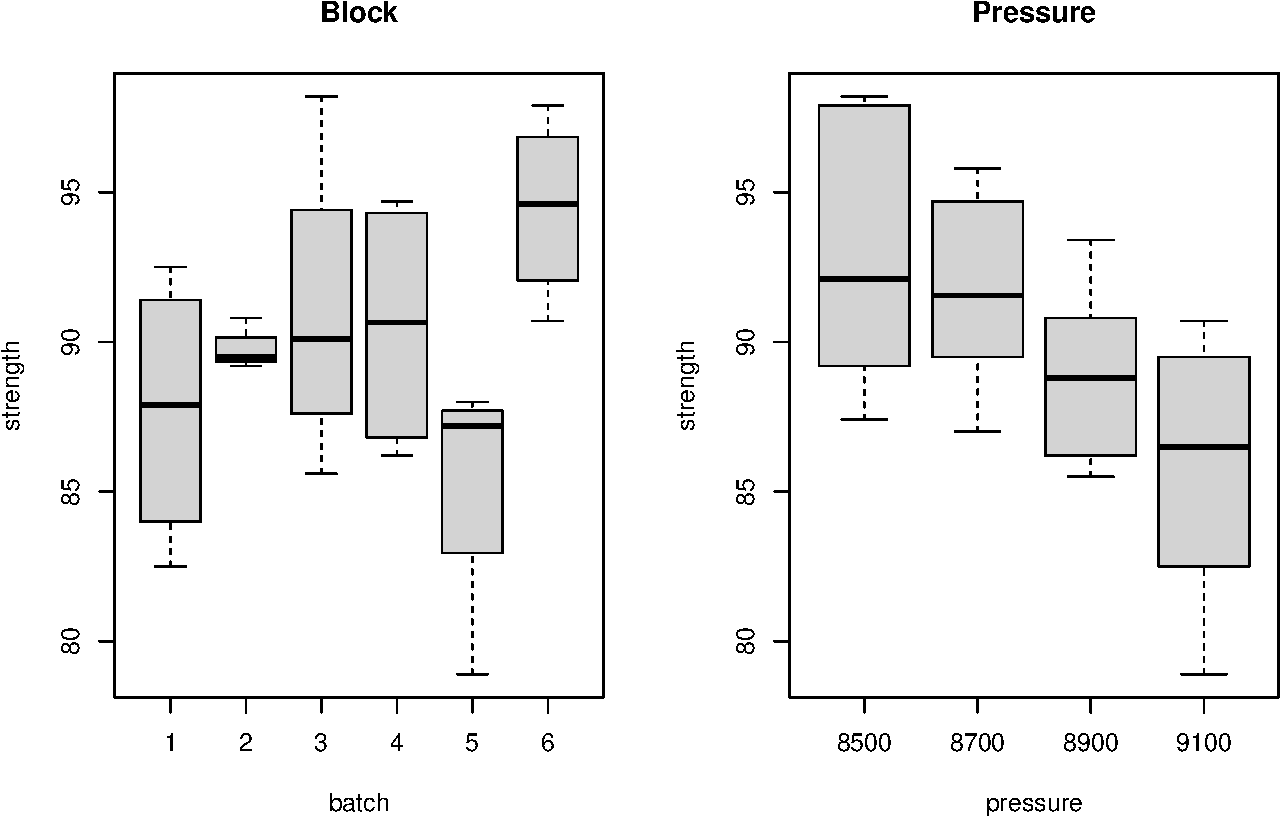
\includegraphics[keepaspectratio]{unit5-factor/crbd_files/figure-pdf/unnamed-chunk-3-1.pdf}}

\textbf{Interaction Plots}

\begin{Shaded}
\begin{Highlighting}[]
\FunctionTok{ggplot}\NormalTok{(graft\_df, }\FunctionTok{aes}\NormalTok{(}\AttributeTok{x =}\NormalTok{ pressure, }\AttributeTok{y =}\NormalTok{ strength, }\AttributeTok{group =}\NormalTok{ batch, }\AttributeTok{color =}\NormalTok{ batch)) }\SpecialCharTok{+}
  \FunctionTok{stat\_summary}\NormalTok{(}\AttributeTok{fun =}\NormalTok{ mean, }\AttributeTok{geom =} \StringTok{"line"}\NormalTok{, }\AttributeTok{size =} \DecValTok{1}\NormalTok{) }\SpecialCharTok{+}
  \FunctionTok{stat\_summary}\NormalTok{(}\AttributeTok{fun =}\NormalTok{ mean, }\AttributeTok{geom =} \StringTok{"point"}\NormalTok{, }\AttributeTok{size =} \DecValTok{3}\NormalTok{) }\SpecialCharTok{+}
  \FunctionTok{labs}\NormalTok{(}
    \AttributeTok{title =} \StringTok{"Interaction Plot: Batch and Pressure"}\NormalTok{,}
    \AttributeTok{x =} \StringTok{"Pressue"}\NormalTok{,}
    \AttributeTok{y =} \StringTok{"Strength"}\NormalTok{,}
    \AttributeTok{color =} \StringTok{"Batch"}
\NormalTok{  ) }\SpecialCharTok{+}
  \FunctionTok{theme\_minimal}\NormalTok{() }\SpecialCharTok{+}
  \FunctionTok{theme}\NormalTok{(}\AttributeTok{plot.title =} \FunctionTok{element\_text}\NormalTok{(}\AttributeTok{hjust =} \FloatTok{0.5}\NormalTok{))}
\end{Highlighting}
\end{Shaded}

\begin{figure}[H]

{\centering \pandocbounded{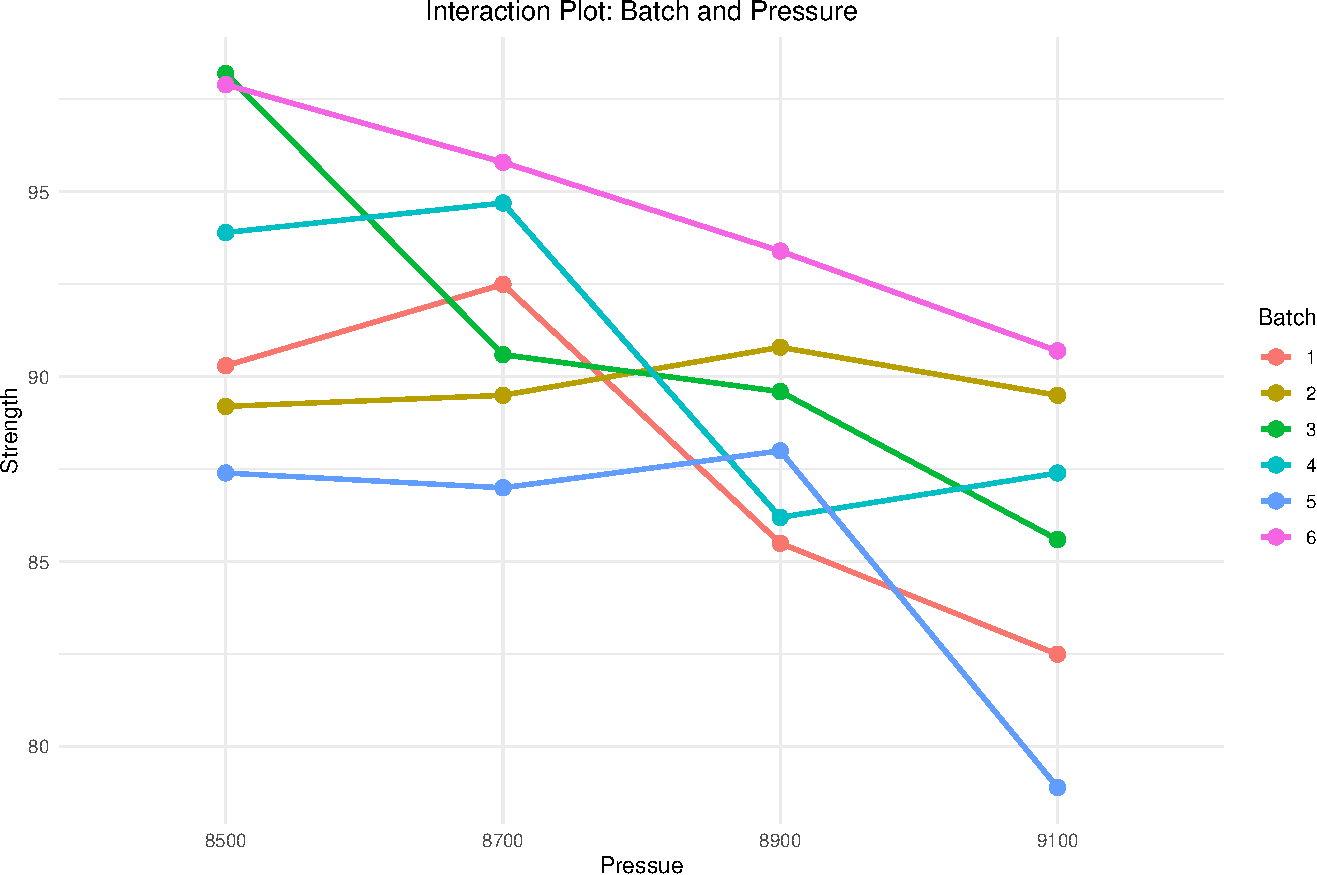
\includegraphics[keepaspectratio]{unit5-factor/crbd_files/figure-pdf/plot-interaction-1.pdf}}

}

\caption{Interaction between Material Type and Temperature.}

\end{figure}%

\begin{verbatim}

### Model Fitting and ANOVA

The model `strength ~ pressure + batch` partitions the total variance into treatment, block, and error components. Our primary interest is in the significance of the `pressure` factor.

::: {.cell}

```{.r .cell-code}
rcbd.fit1 <- aov(strength ~ pressure + batch, data = graft_df)
anova(rcbd.fit1)
\end{verbatim}

\begin{verbatim}
Analysis of Variance Table

Response: strength
          Df Sum Sq Mean Sq F value   Pr(>F)   
pressure   3 178.17  59.390  8.1071 0.001916 **
batch      5 192.25  38.450  5.2487 0.005532 **
Residuals 15 109.89   7.326                    
---
Signif. codes:  0 '***' 0.001 '**' 0.01 '*' 0.05 '.' 0.1 ' ' 1
\end{verbatim}

:::

The small p-value for \texttt{pressure} (0.0019) provides strong
evidence that extrusion pressure significantly affects graft strength
after accounting for batch differences.

\subsubsection{Model Adequacy Checks}\label{model-adequacy-checks}

The assumptions for an RCBD are the same as for a CRD. We perform the
same diagnostic checks.

\begin{Shaded}
\begin{Highlighting}[]
\NormalTok{rcbd.r1 }\OtherTok{\textless{}{-}} \FunctionTok{rstudent}\NormalTok{(rcbd.fit1)}
\NormalTok{rcbd.fitted1 }\OtherTok{\textless{}{-}} \FunctionTok{fitted.values}\NormalTok{(rcbd.fit1)}

\FunctionTok{qqnorm}\NormalTok{(rcbd.r1, }\AttributeTok{main =} \StringTok{"Normal Q{-}Q Plot"}\NormalTok{)}
\FunctionTok{qqline}\NormalTok{(rcbd.r1)}
\FunctionTok{plot}\NormalTok{(rcbd.fitted1, rcbd.r1, }\AttributeTok{ylab =} \StringTok{"Standardized residuals"}\NormalTok{, }
     \AttributeTok{xlab =} \StringTok{"Fitted values"}\NormalTok{, }\AttributeTok{main =} \StringTok{"Residuals vs. Fitted"}\NormalTok{)}
\FunctionTok{abline}\NormalTok{(}\AttributeTok{h =} \DecValTok{0}\NormalTok{)}
\FunctionTok{plot}\NormalTok{(graft\_df}\SpecialCharTok{$}\NormalTok{pressure, rcbd.r1, }\AttributeTok{ylab =} \StringTok{"Standardized residuals"}\NormalTok{, }
     \AttributeTok{xlab =} \StringTok{"Extrusion pressure"}\NormalTok{, }\AttributeTok{main =} \StringTok{"Residuals vs. Treatment"}\NormalTok{)}
\FunctionTok{abline}\NormalTok{(}\AttributeTok{h =} \DecValTok{0}\NormalTok{)}
\FunctionTok{plot}\NormalTok{(graft\_df}\SpecialCharTok{$}\NormalTok{batch, rcbd.r1, }\AttributeTok{ylab =} \StringTok{"Standardized residuals"}\NormalTok{, }
     \AttributeTok{xlab =} \StringTok{"Batches of raw material"}\NormalTok{, }\AttributeTok{main =} \StringTok{"Residuals vs. Block"}\NormalTok{)}
\FunctionTok{abline}\NormalTok{(}\AttributeTok{h =} \DecValTok{0}\NormalTok{)}
\end{Highlighting}
\end{Shaded}

\begin{figure}

\begin{minipage}{0.50\linewidth}

\begin{figure}[H]

{\centering \pandocbounded{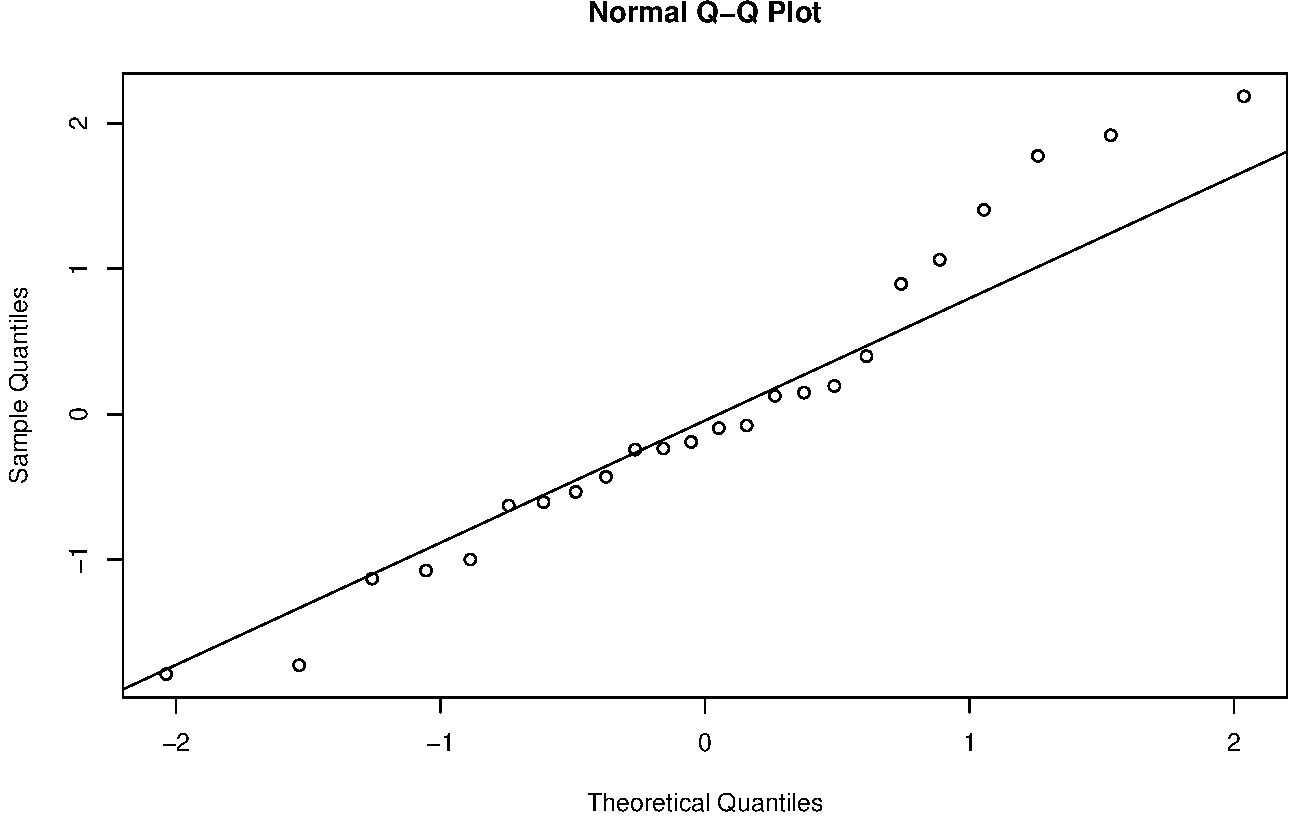
\includegraphics[keepaspectratio]{unit5-factor/crbd_files/figure-pdf/plot-diagnostics-rcbd-1.pdf}}

}

\subcaption{Normal Q-Q Plot}

\end{figure}%

\end{minipage}%
%
\begin{minipage}{0.50\linewidth}

\begin{figure}[H]

{\centering \pandocbounded{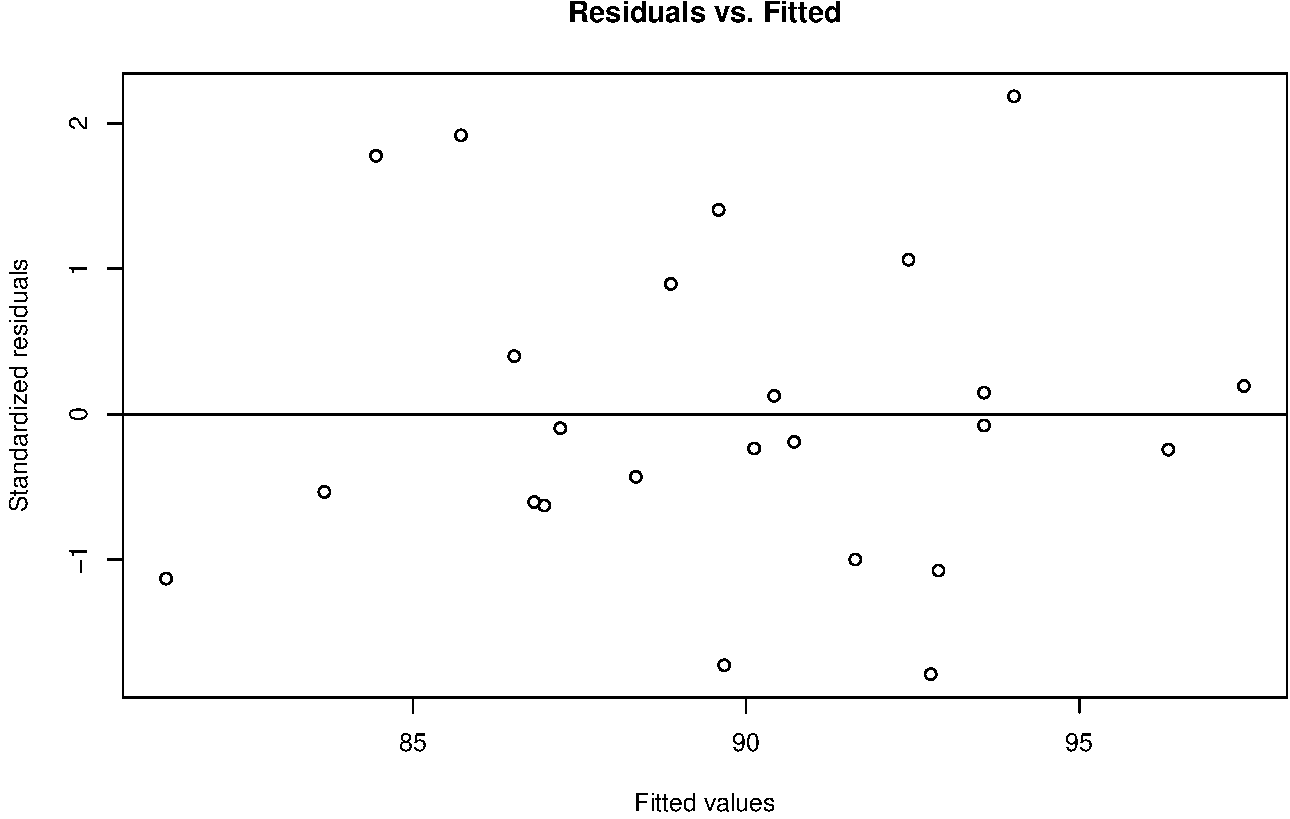
\includegraphics[keepaspectratio]{unit5-factor/crbd_files/figure-pdf/plot-diagnostics-rcbd-2.pdf}}

}

\subcaption{Residuals vs.~Fitted Values}

\end{figure}%

\end{minipage}%
\newline
\begin{minipage}{0.50\linewidth}

\begin{figure}[H]

{\centering \pandocbounded{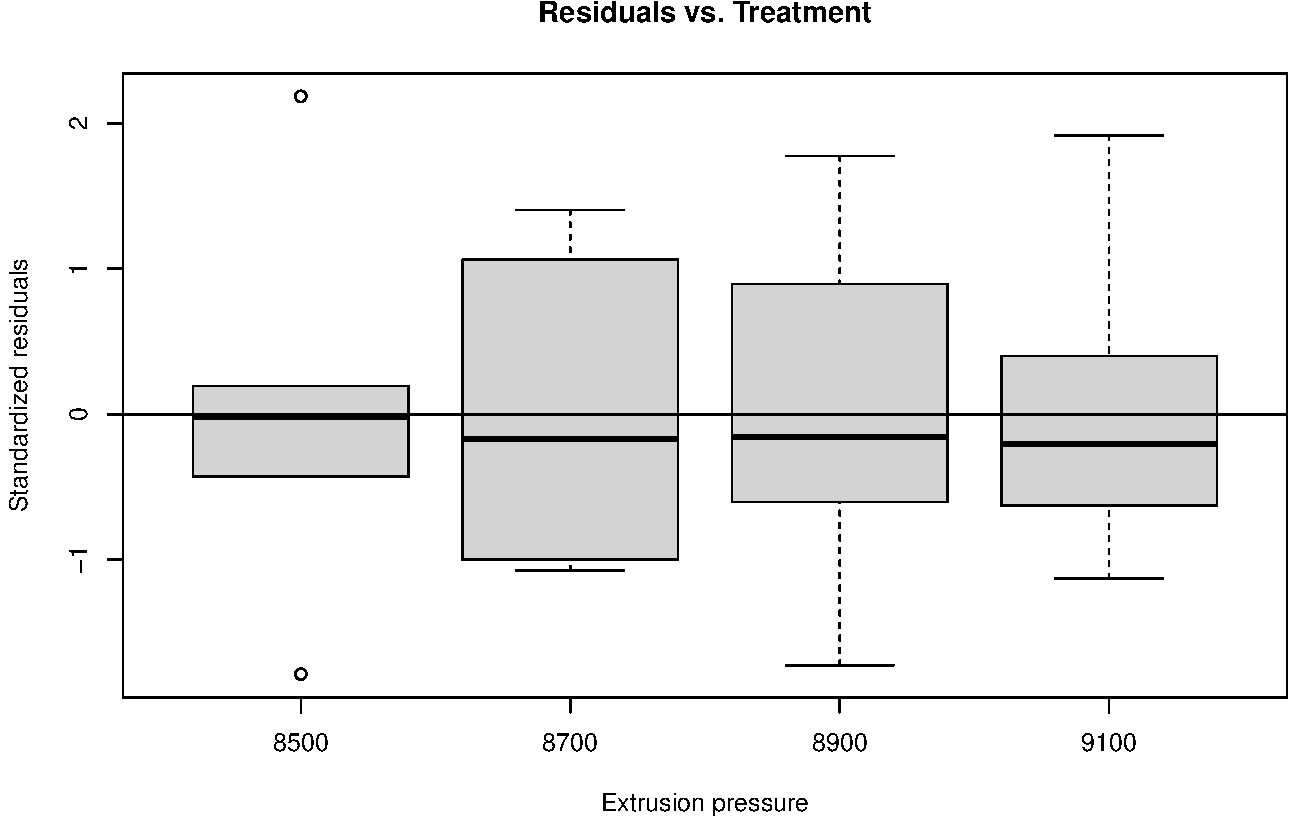
\includegraphics[keepaspectratio]{unit5-factor/crbd_files/figure-pdf/plot-diagnostics-rcbd-3.pdf}}

}

\subcaption{Residuals vs.~Treatment (Pressure)}

\end{figure}%

\end{minipage}%
%
\begin{minipage}{0.50\linewidth}

\begin{figure}[H]

{\centering \pandocbounded{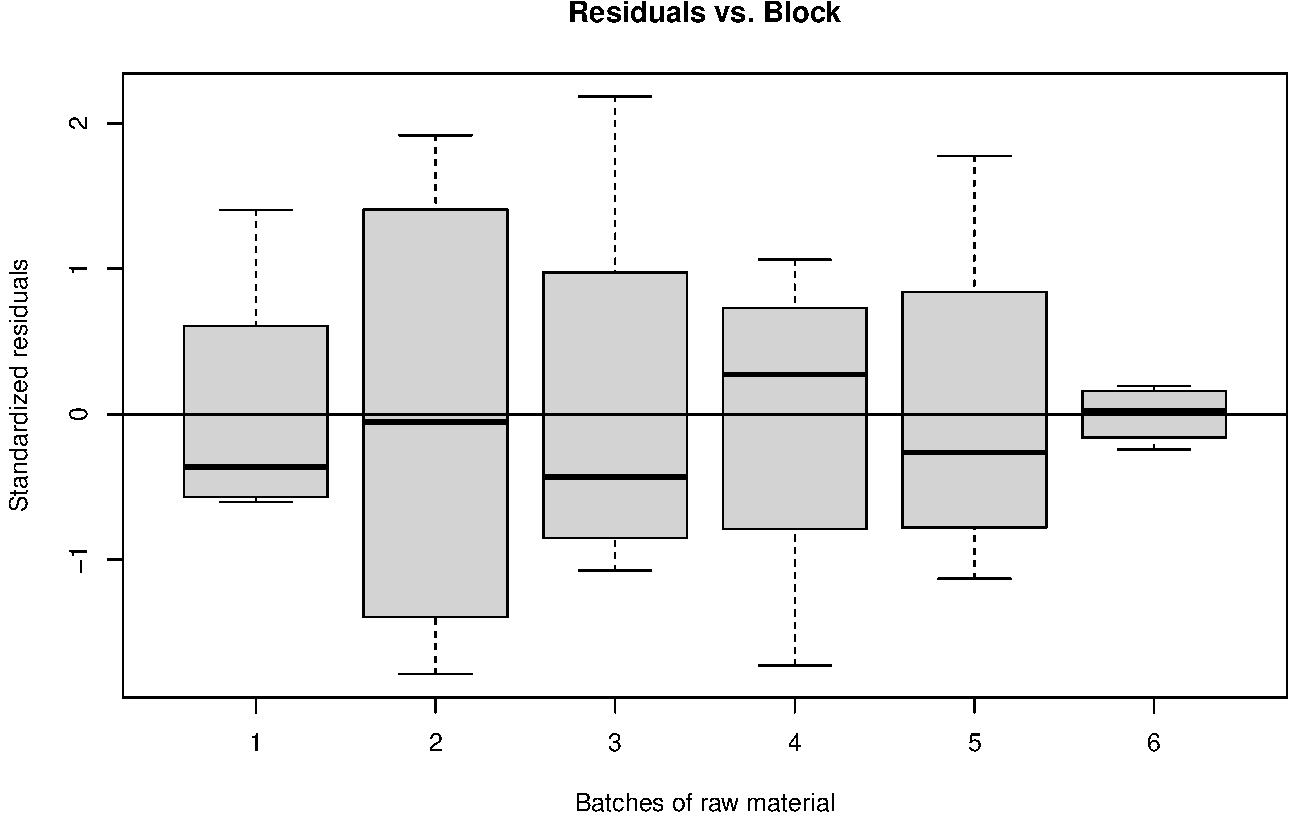
\includegraphics[keepaspectratio]{unit5-factor/crbd_files/figure-pdf/plot-diagnostics-rcbd-4.pdf}}

}

\subcaption{Residuals vs.~Block (Batch)}

\end{figure}%

\end{minipage}%

\end{figure}%

\subsubsection{Pairwise Comparisons}\label{pairwise-comparisons-1}

Again, since the treatment factor (\texttt{pressure}) is significant, we
perform post-hoc tests.

\paragraph{Tukey's HSD Test}\label{tukeys-hsd-test-1}

Tukey's HSD compares all pairs of treatment levels while controlling the
family-wise error rate.

\begin{Shaded}
\begin{Highlighting}[]
\FunctionTok{TukeyHSD}\NormalTok{(rcbd.fit1, }\AttributeTok{which =} \StringTok{"pressure"}\NormalTok{)}
\end{Highlighting}
\end{Shaded}

\begin{verbatim}
  Tukey multiple comparisons of means
    95% family-wise confidence level

Fit: aov(formula = strength ~ pressure + batch, data = graft_df)

$pressure
               diff        lwr       upr     p adj
8700-8500 -1.133333  -5.637161  3.370495 0.8854831
8900-8500 -3.900000  -8.403828  0.603828 0.1013084
9100-8500 -7.050000 -11.553828 -2.546172 0.0020883
8900-8700 -2.766667  -7.270495  1.737161 0.3245644
9100-8700 -5.916667 -10.420495 -1.412839 0.0086667
9100-8900 -3.150000  -7.653828  1.353828 0.2257674
\end{verbatim}

\paragraph{Fisher's LSD Test}\label{fishers-lsd-test-1}

The \texttt{LSD.test()} function from the \texttt{agricolae} package
correctly handles the error structure of an RCBD.

\begin{Shaded}
\begin{Highlighting}[]
\CommentTok{\# install.packages("agricolae")}
\FunctionTok{library}\NormalTok{(agricolae)}

\NormalTok{out }\OtherTok{\textless{}{-}} \FunctionTok{LSD.test}\NormalTok{(rcbd.fit1, }\AttributeTok{trt =} \StringTok{"pressure"}\NormalTok{, }\AttributeTok{p.adj =} \StringTok{"none"}\NormalTok{, }\AttributeTok{group =} \ConstantTok{FALSE}\NormalTok{)}
\FunctionTok{print}\NormalTok{(out}\SpecialCharTok{$}\NormalTok{comparison)}
\end{Highlighting}
\end{Shaded}

\begin{verbatim}
            difference pvalue signif.        LCL       UCL
8500 - 8700   1.133333 0.4795         -2.1974047  4.464071
8500 - 8900   3.900000 0.0247       *  0.5692620  7.230738
8500 - 9100   7.050000 0.0004     ***  3.7192620 10.380738
8700 - 8900   2.766667 0.0970       . -0.5640714  6.097405
8700 - 9100   5.916667 0.0018      **  2.5859286  9.247405
8900 - 9100   3.150000 0.0621       . -0.1807380  6.480738
\end{verbatim}

\section{Two-Factor Factorial Design}\label{two-factor-factorial-design}

\section{Battery Design Experiment}\label{battery-design-experiment}

This analysis explores data from a \textbf{two-factor factorial
experiment} designed to assess the lifespan of a battery. The experiment
investigates two factors: \textbf{material type} (with 3 levels) and
\textbf{operating temperature} (with 3 levels: 15°C, 70°C, and 125°C).
The primary goal is to understand not only how each factor individually
affects battery life but, more importantly, whether the effect of
temperature depends on the material type used. This combined effect is
known as an \textbf{interaction}.

\section{Data Setup and Preparation}\label{data-setup-and-preparation}

First, we organize the raw data into a structured \texttt{data.frame}.
This is a best practice in R that makes the data easier to manage and
the code more readable. We create columns for the response variable
\texttt{life} and the two factors, \texttt{material} and
\texttt{temperature}, ensuring they are treated as categorical variables
(factors) for the analysis.

\begin{Shaded}
\begin{Highlighting}[]
\CommentTok{\# Response variable: battery life}
\NormalTok{life }\OtherTok{\textless{}{-}} \FunctionTok{c}\NormalTok{(}\DecValTok{130}\NormalTok{,}\DecValTok{155}\NormalTok{,}\DecValTok{74}\NormalTok{,}\DecValTok{180}\NormalTok{,  }\DecValTok{34}\NormalTok{,}\DecValTok{40}\NormalTok{,}\DecValTok{80}\NormalTok{,}\DecValTok{75}\NormalTok{,   }\DecValTok{20}\NormalTok{,}\DecValTok{70}\NormalTok{,}\DecValTok{82}\NormalTok{,}\DecValTok{58}\NormalTok{,}
          \DecValTok{150}\NormalTok{,}\DecValTok{188}\NormalTok{,}\DecValTok{159}\NormalTok{,}\DecValTok{126}\NormalTok{, }\DecValTok{136}\NormalTok{,}\DecValTok{122}\NormalTok{,}\DecValTok{106}\NormalTok{,}\DecValTok{115}\NormalTok{, }\DecValTok{25}\NormalTok{,}\DecValTok{70}\NormalTok{,}\DecValTok{58}\NormalTok{,}\DecValTok{45}\NormalTok{,}
          \DecValTok{138}\NormalTok{,}\DecValTok{110}\NormalTok{,}\DecValTok{168}\NormalTok{,}\DecValTok{160}\NormalTok{, }\DecValTok{174}\NormalTok{,}\DecValTok{120}\NormalTok{,}\DecValTok{150}\NormalTok{,}\DecValTok{139}\NormalTok{, }\DecValTok{96}\NormalTok{,}\DecValTok{104}\NormalTok{,}\DecValTok{82}\NormalTok{,}\DecValTok{60}\NormalTok{)}

\CommentTok{\# Create the data frame}
\NormalTok{battery\_df }\OtherTok{\textless{}{-}} \FunctionTok{data.frame}\NormalTok{(}
  \AttributeTok{life =}\NormalTok{ life,}
  \AttributeTok{material =} \FunctionTok{factor}\NormalTok{(}\FunctionTok{rep}\NormalTok{(}\DecValTok{1}\SpecialCharTok{:}\DecValTok{3}\NormalTok{, }\AttributeTok{each =} \DecValTok{12}\NormalTok{)),}
  \AttributeTok{temperature =} \FunctionTok{factor}\NormalTok{(}\FunctionTok{rep}\NormalTok{(}\FunctionTok{rep}\NormalTok{(}\FunctionTok{c}\NormalTok{(}\DecValTok{15}\NormalTok{, }\DecValTok{70}\NormalTok{, }\DecValTok{125}\NormalTok{), }\AttributeTok{each =} \DecValTok{4}\NormalTok{), }\DecValTok{3}\NormalTok{))}
\NormalTok{)}

\CommentTok{\# Preview the data}
\NormalTok{battery\_df}
\end{Highlighting}
\end{Shaded}

\begin{verbatim}
   life material temperature
1   130        1          15
2   155        1          15
3    74        1          15
4   180        1          15
5    34        1          70
6    40        1          70
7    80        1          70
8    75        1          70
9    20        1         125
10   70        1         125
11   82        1         125
12   58        1         125
13  150        2          15
14  188        2          15
15  159        2          15
16  126        2          15
17  136        2          70
18  122        2          70
19  106        2          70
20  115        2          70
21   25        2         125
22   70        2         125
23   58        2         125
24   45        2         125
25  138        3          15
26  110        3          15
27  168        3          15
28  160        3          15
29  174        3          70
30  120        3          70
31  150        3          70
32  139        3          70
33   96        3         125
34  104        3         125
35   82        3         125
36   60        3         125
\end{verbatim}

\section{Exploratory Data Analysis and
Visualization}\label{exploratory-data-analysis-and-visualization}

Before fitting a formal model, we visualize the data to get an intuition
for the relationships between the factors and the response.

\section{Boxplots of Main Effects}\label{boxplots-of-main-effects}

Boxplots are excellent for examining the distribution of battery life
for each level of our factors independently. This gives us a preliminary
look at the \textbf{main effects}---the individual impact of material
type and temperature.

\begin{Shaded}
\begin{Highlighting}[]
\FunctionTok{library}\NormalTok{(ggplot2)}

\CommentTok{\# Boxplot for Material Type}
\FunctionTok{ggplot}\NormalTok{(battery\_df, }\FunctionTok{aes}\NormalTok{(}\AttributeTok{x =}\NormalTok{ material, }\AttributeTok{y =}\NormalTok{ life, }\AttributeTok{fill =}\NormalTok{ material)) }\SpecialCharTok{+}
  \FunctionTok{geom\_boxplot}\NormalTok{() }\SpecialCharTok{+}
  \FunctionTok{labs}\NormalTok{(}\AttributeTok{title =} \StringTok{"Battery Life by Material Type"}\NormalTok{, }\AttributeTok{x =} \StringTok{"Material Type"}\NormalTok{, }\AttributeTok{y =} \StringTok{"Life (hours)"}\NormalTok{) }\SpecialCharTok{+}
  \FunctionTok{theme\_minimal}\NormalTok{() }\SpecialCharTok{+}
  \FunctionTok{theme}\NormalTok{(}\AttributeTok{legend.position =} \StringTok{"none"}\NormalTok{)}
\CommentTok{\# Boxplot for Temperature}
\FunctionTok{ggplot}\NormalTok{(battery\_df, }\FunctionTok{aes}\NormalTok{(}\AttributeTok{x =}\NormalTok{ temperature, }\AttributeTok{y =}\NormalTok{ life, }\AttributeTok{fill =}\NormalTok{ temperature)) }\SpecialCharTok{+}
  \FunctionTok{geom\_boxplot}\NormalTok{() }\SpecialCharTok{+}
  \FunctionTok{labs}\NormalTok{(}\AttributeTok{title =} \StringTok{"Battery Life by Temperature"}\NormalTok{, }\AttributeTok{x =} \StringTok{"Temperature (°C)"}\NormalTok{, }\AttributeTok{y =} \StringTok{"Life (hours)"}\NormalTok{) }\SpecialCharTok{+}
  \FunctionTok{theme\_minimal}\NormalTok{() }\SpecialCharTok{+}
  \FunctionTok{theme}\NormalTok{(}\AttributeTok{legend.position =} \StringTok{"none"}\NormalTok{)}
\end{Highlighting}
\end{Shaded}

\begin{figure}

\begin{minipage}{0.50\linewidth}

\begin{figure}[H]

{\centering \pandocbounded{\includegraphics[keepaspectratio]{unit6-factorial/factorial_files/figure-pdf/plot-boxplots-1.pdf}}

}

\subcaption{Distribution of Battery Life by Material and Temperature.}

\end{figure}%

\end{minipage}%
%
\begin{minipage}{0.50\linewidth}

\begin{figure}[H]

{\centering \pandocbounded{\includegraphics[keepaspectratio]{unit6-factorial/factorial_files/figure-pdf/plot-boxplots-2.pdf}}

}

\subcaption{Distribution of Battery Life by Material and Temperature.}

\end{figure}%

\end{minipage}%

\end{figure}%

\section{Interaction Plot}\label{interaction-plot}

The most crucial plot for a factorial experiment is the
\textbf{interaction plot}. It displays the mean battery life for each
combination of material and temperature. If the lines are parallel, it
suggests there is no interaction. If the lines are not parallel (i.e.,
they cross or diverge), it indicates that the effect of temperature on
battery life is different for each material type, signaling a likely
interaction.

\begin{Shaded}
\begin{Highlighting}[]
\FunctionTok{ggplot}\NormalTok{(battery\_df, }\FunctionTok{aes}\NormalTok{(}\AttributeTok{x =}\NormalTok{ temperature, }\AttributeTok{y =}\NormalTok{ life, }\AttributeTok{group =}\NormalTok{ material, }\AttributeTok{color =}\NormalTok{ material)) }\SpecialCharTok{+}
  \FunctionTok{stat\_summary}\NormalTok{(}\AttributeTok{fun =}\NormalTok{ mean, }\AttributeTok{geom =} \StringTok{"line"}\NormalTok{, }\AttributeTok{size =} \DecValTok{1}\NormalTok{) }\SpecialCharTok{+}
  \FunctionTok{stat\_summary}\NormalTok{(}\AttributeTok{fun =}\NormalTok{ mean, }\AttributeTok{geom =} \StringTok{"point"}\NormalTok{, }\AttributeTok{size =} \DecValTok{3}\NormalTok{) }\SpecialCharTok{+}
  \FunctionTok{labs}\NormalTok{(}
    \AttributeTok{title =} \StringTok{"Interaction Plot: Material Type and Temperature"}\NormalTok{,}
    \AttributeTok{x =} \StringTok{"Temperature (°C)"}\NormalTok{,}
    \AttributeTok{y =} \StringTok{"Average Battery Life (hours)"}\NormalTok{,}
    \AttributeTok{color =} \StringTok{"Material Type"}
\NormalTok{  ) }\SpecialCharTok{+}
  \FunctionTok{theme\_minimal}\NormalTok{() }\SpecialCharTok{+}
  \FunctionTok{theme}\NormalTok{(}\AttributeTok{plot.title =} \FunctionTok{element\_text}\NormalTok{(}\AttributeTok{hjust =} \FloatTok{0.5}\NormalTok{))}
\end{Highlighting}
\end{Shaded}

\begin{figure}[H]

{\centering \pandocbounded{\includegraphics[keepaspectratio]{unit6-factorial/factorial_files/figure-pdf/plot-interaction-1.pdf}}

}

\caption{Interaction between Material Type and Temperature.}

\end{figure}%

The non-parallel lines in the plot strongly suggest that a significant
interaction effect is present. Specifically, the performance of Material
3 drops less dramatically with increasing temperature compared to
Materials 1 and 2.

\section{Model Fitting and Analysis of Variance
(ANOVA)}\label{model-fitting-and-analysis-of-variance-anova}

We now fit a linear model to formally test the significance of the main
effects and the interaction term. The model
\texttt{life\ \textasciitilde{}\ material\ *\ temperature} is shorthand
for
\texttt{life\ \textasciitilde{}\ material\ +\ temperature\ +\ material:temperature}.
We use a sum-to-zero contrast (\texttt{contr.sum}) for balanced
interpretation of the effects. The \textbf{ANOVA table} will tell us if
the variation caused by our factors is statistically significant
compared to the random variation in the data.

\begin{Shaded}
\begin{Highlighting}[]
\CommentTok{\# Fit the full factorial model}
\NormalTok{battery\_fit }\OtherTok{\textless{}{-}} \FunctionTok{lm}\NormalTok{(life }\SpecialCharTok{\textasciitilde{}}\NormalTok{ material }\SpecialCharTok{*}\NormalTok{ temperature, }
                  \AttributeTok{data =}\NormalTok{ battery\_df,}
                  \AttributeTok{contrasts =} \FunctionTok{list}\NormalTok{(}\AttributeTok{material =}\NormalTok{ contr.sum, }\AttributeTok{temperature =}\NormalTok{ contr.sum))}

\FunctionTok{summary}\NormalTok{(battery\_fit)}
\end{Highlighting}
\end{Shaded}

\begin{verbatim}

Call:
lm(formula = life ~ material * temperature, data = battery_df, 
    contrasts = list(material = contr.sum, temperature = contr.sum))

Residuals:
    Min      1Q  Median      3Q     Max 
-60.750 -14.625   1.375  17.938  45.250 

Coefficients:
                       Estimate Std. Error t value Pr(>|t|)    
(Intercept)             105.528      4.331  24.367  < 2e-16 ***
material1               -22.361      6.125  -3.651  0.00111 ** 
material2                 2.806      6.125   0.458  0.65057    
temperature1             39.306      6.125   6.418  7.1e-07 ***
temperature2              2.056      6.125   0.336  0.73975    
material1:temperature1   12.278      8.662   1.417  0.16778    
material2:temperature1    8.111      8.662   0.936  0.35735    
material1:temperature2  -27.972      8.662  -3.229  0.00325 ** 
material2:temperature2    9.361      8.662   1.081  0.28936    
---
Signif. codes:  0 '***' 0.001 '**' 0.01 '*' 0.05 '.' 0.1 ' ' 1

Residual standard error: 25.98 on 27 degrees of freedom
Multiple R-squared:  0.7652,    Adjusted R-squared:  0.6956 
F-statistic:    11 on 8 and 27 DF,  p-value: 9.426e-07
\end{verbatim}

\begin{Shaded}
\begin{Highlighting}[]
\CommentTok{\# Generate the ANOVA table}
\FunctionTok{anova}\NormalTok{(battery\_fit)}
\end{Highlighting}
\end{Shaded}

\begin{verbatim}
Analysis of Variance Table

Response: life
                     Df Sum Sq Mean Sq F value    Pr(>F)    
material              2  10684  5341.9  7.9114  0.001976 ** 
temperature           2  39119 19559.4 28.9677 1.909e-07 ***
material:temperature  4   9614  2403.4  3.5595  0.018611 *  
Residuals            27  18231   675.2                      
---
Signif. codes:  0 '***' 0.001 '**' 0.01 '*' 0.05 '.' 0.1 ' ' 1
\end{verbatim}

The ANOVA table shows very small p-values (\texttt{Pr(\textgreater{}F)})
for \texttt{material}, \texttt{temperature}, and, most importantly, the
\texttt{material:temperature} interaction. This confirms our visual
inspection: all effects are statistically significant. \textbf{Because
the interaction is significant, our interpretation should focus on the
interaction itself rather than the main effects in isolation.}

\section{Model Adequacy Checks}\label{model-adequacy-checks-1}

The validity of our ANOVA results depends on the model's residuals
meeting certain assumptions (normality, constant variance,
independence). We check these with diagnostic plots.

\begin{Shaded}
\begin{Highlighting}[]
\CommentTok{\# Extract standardized residuals and fitted values}
\NormalTok{battery\_fit\_diag }\OtherTok{\textless{}{-}} \FunctionTok{data.frame}\NormalTok{(}
  \AttributeTok{residuals =} \FunctionTok{rstandard}\NormalTok{(battery\_fit),}
  \AttributeTok{fitted =} \FunctionTok{fitted.values}\NormalTok{(battery\_fit)}
\NormalTok{)}

\CommentTok{\# Normal Q{-}Q Plot}
\NormalTok{p1 }\OtherTok{\textless{}{-}} \FunctionTok{ggplot}\NormalTok{(battery\_fit\_diag, }\FunctionTok{aes}\NormalTok{(}\AttributeTok{sample =}\NormalTok{ residuals)) }\SpecialCharTok{+}
  \FunctionTok{stat\_qq}\NormalTok{() }\SpecialCharTok{+}
  \FunctionTok{stat\_qq\_line}\NormalTok{() }\SpecialCharTok{+}
  \FunctionTok{labs}\NormalTok{(}\AttributeTok{title =} \StringTok{"Normal Q{-}Q Plot"}\NormalTok{, }\AttributeTok{x =} \StringTok{"Theoretical Quantiles"}\NormalTok{, }\AttributeTok{y =} \StringTok{"Standardized Residuals"}\NormalTok{) }\SpecialCharTok{+}
  \FunctionTok{theme\_minimal}\NormalTok{()}

\CommentTok{\# Residuals vs. Fitted Plot}
\NormalTok{p2 }\OtherTok{\textless{}{-}} \FunctionTok{ggplot}\NormalTok{(battery\_fit\_diag, }\FunctionTok{aes}\NormalTok{(}\AttributeTok{x =}\NormalTok{ fitted, }\AttributeTok{y =}\NormalTok{ residuals)) }\SpecialCharTok{+}
  \FunctionTok{geom\_point}\NormalTok{() }\SpecialCharTok{+}
  \FunctionTok{geom\_hline}\NormalTok{(}\AttributeTok{yintercept =} \DecValTok{0}\NormalTok{, }\AttributeTok{linetype =} \StringTok{"dashed"}\NormalTok{, }\AttributeTok{color =} \StringTok{"red"}\NormalTok{) }\SpecialCharTok{+}
  \FunctionTok{labs}\NormalTok{(}\AttributeTok{title =} \StringTok{"Residuals vs. Fitted Values"}\NormalTok{, }\AttributeTok{x =} \StringTok{"Fitted Values"}\NormalTok{, }\AttributeTok{y =} \StringTok{"Standardized Residuals"}\NormalTok{) }\SpecialCharTok{+}
  \FunctionTok{theme\_minimal}\NormalTok{()}

\NormalTok{p1 }
\NormalTok{p2}
\end{Highlighting}
\end{Shaded}

\begin{figure}

\begin{minipage}{0.50\linewidth}

\begin{figure}[H]

{\centering \pandocbounded{\includegraphics[keepaspectratio]{unit6-factorial/factorial_files/figure-pdf/plot-diagnostics-1.pdf}}

}

\subcaption{Diagnostic plots for the battery life model.}

\end{figure}%

\end{minipage}%
%
\begin{minipage}{0.50\linewidth}

\begin{figure}[H]

{\centering \pandocbounded{\includegraphics[keepaspectratio]{unit6-factorial/factorial_files/figure-pdf/plot-diagnostics-2.pdf}}

}

\subcaption{Diagnostic plots for the battery life model.}

\end{figure}%

\end{minipage}%

\end{figure}%

The Normal Q-Q plot shows the points falling roughly along the line,
suggesting the normality assumption is met. The Residuals vs.~Fitted
plot shows a random scatter of points around the zero line, indicating
that the variance is reasonably constant. The model assumptions appear
to be satisfied.

\section{Post-Hoc Analysis: Pairwise
Comparisons}\label{post-hoc-analysis-pairwise-comparisons}

Since the interaction is significant, we must compare the means of the
nine specific treatment combinations (3 materials × 3 temperatures).
Simply comparing the average effect of Material 1 vs.~Material 2 would
be misleading, as that difference depends on the temperature.

\section{Tukey's HSD Test}\label{tukeys-hsd-test-2}

\textbf{Tukey's Honest Significant Difference (HSD)} test is a post-hoc
test that compares all possible pairs of means while controlling the
family-wise error rate. We apply it to an \texttt{aov} model object. The
output for the \texttt{material:temperature} interaction shows which
specific combinations are significantly different from one another.

\begin{Shaded}
\begin{Highlighting}[]
\CommentTok{\# Fit the model using aov() for Tukey\textquotesingle{}s test}
\NormalTok{battery\_aov }\OtherTok{\textless{}{-}} \FunctionTok{aov}\NormalTok{(life }\SpecialCharTok{\textasciitilde{}}\NormalTok{ material }\SpecialCharTok{*}\NormalTok{ temperature, }\AttributeTok{data =}\NormalTok{ battery\_df)}

\CommentTok{\# Perform Tukey\textquotesingle{}s HSD test}
\FunctionTok{TukeyHSD}\NormalTok{(battery\_aov)}
\end{Highlighting}
\end{Shaded}

\begin{verbatim}
  Tukey multiple comparisons of means
    95% family-wise confidence level

Fit: aov(formula = life ~ material * temperature, data = battery_df)

$material
        diff       lwr      upr     p adj
2-1 25.16667 -1.135677 51.46901 0.0627571
3-1 41.91667 15.614323 68.21901 0.0014162
3-2 16.75000 -9.552344 43.05234 0.2717815

$temperature
            diff        lwr       upr     p adj
70-15  -37.25000  -63.55234 -10.94766 0.0043788
125-15 -80.66667 -106.96901 -54.36432 0.0000001
125-70 -43.41667  -69.71901 -17.11432 0.0009787

$`material:temperature`
               diff         lwr        upr     p adj
2:15-1:15     21.00  -40.823184  82.823184 0.9616404
3:15-1:15      9.25  -52.573184  71.073184 0.9998527
1:70-1:15    -77.50 -139.323184 -15.676816 0.0065212
2:70-1:15    -15.00  -76.823184  46.823184 0.9953182
3:70-1:15     11.00  -50.823184  72.823184 0.9994703
1:125-1:15   -77.25 -139.073184 -15.426816 0.0067471
2:125-1:15   -85.25 -147.073184 -23.426816 0.0022351
3:125-1:15   -49.25 -111.073184  12.573184 0.2016535
3:15-2:15    -11.75  -73.573184  50.073184 0.9991463
1:70-2:15    -98.50 -160.323184 -36.676816 0.0003449
2:70-2:15    -36.00  -97.823184  25.823184 0.5819453
3:70-2:15    -10.00  -71.823184  51.823184 0.9997369
1:125-2:15   -98.25 -160.073184 -36.426816 0.0003574
2:125-2:15  -106.25 -168.073184 -44.426816 0.0001152
3:125-2:15   -70.25 -132.073184  -8.426816 0.0172076
1:70-3:15    -86.75 -148.573184 -24.926816 0.0018119
2:70-3:15    -24.25  -86.073184  37.573184 0.9165175
3:70-3:15      1.75  -60.073184  63.573184 1.0000000
1:125-3:15   -86.50 -148.323184 -24.676816 0.0018765
2:125-3:15   -94.50 -156.323184 -32.676816 0.0006078
3:125-3:15   -58.50 -120.323184   3.323184 0.0742711
2:70-1:70     62.50    0.676816 124.323184 0.0460388
3:70-1:70     88.50   26.676816 150.323184 0.0014173
1:125-1:70     0.25  -61.573184  62.073184 1.0000000
2:125-1:70    -7.75  -69.573184  54.073184 0.9999614
3:125-1:70    28.25  -33.573184  90.073184 0.8281938
3:70-2:70     26.00  -35.823184  87.823184 0.8822881
1:125-2:70   -62.25 -124.073184  -0.426816 0.0474675
2:125-2:70   -70.25 -132.073184  -8.426816 0.0172076
3:125-2:70   -34.25  -96.073184  27.573184 0.6420441
1:125-3:70   -88.25 -150.073184 -26.426816 0.0014679
2:125-3:70   -96.25 -158.073184 -34.426816 0.0004744
3:125-3:70   -60.25 -122.073184   1.573184 0.0604247
2:125-1:125   -8.00  -69.823184  53.823184 0.9999508
3:125-1:125   28.00  -33.823184  89.823184 0.8347331
3:125-2:125   36.00  -25.823184  97.823184 0.5819453
\end{verbatim}

\section{Fisher's LSD Method}\label{fishers-lsd-method}

The \textbf{Fisher's Least Significant Difference (LSD)} method is
another option for pairwise comparisons. To test the interaction means,
we must specify both factors in the \texttt{trt} argument.

\begin{Shaded}
\begin{Highlighting}[]
\FunctionTok{library}\NormalTok{(agricolae)}

\CommentTok{\# Perform LSD test on the interaction term}
\NormalTok{lsd\_results }\OtherTok{\textless{}{-}} \FunctionTok{LSD.test}\NormalTok{(battery\_aov, }\AttributeTok{trt =} \FunctionTok{c}\NormalTok{(}\StringTok{"material"}\NormalTok{, }\StringTok{"temperature"}\NormalTok{),}
                        \AttributeTok{p.adj =} \StringTok{"none"}\NormalTok{, }\AttributeTok{group =} \ConstantTok{FALSE}\NormalTok{)}

\CommentTok{\# Print the comparison table}
\FunctionTok{print}\NormalTok{(lsd\_results}\SpecialCharTok{$}\NormalTok{comparison)}
\end{Highlighting}
\end{Shaded}

\begin{verbatim}
              difference pvalue signif.         LCL        UCL
1:125 - 1:15      -77.25 0.0003     *** -114.950479 -39.549521
1:125 - 1:70        0.25 0.9892          -37.450479  37.950479
1:125 - 2:125       8.00 0.6667          -29.700479  45.700479
1:125 - 2:15      -98.25 0.0000     *** -135.950479 -60.549521
1:125 - 2:70      -62.25 0.0022      **  -99.950479 -24.549521
1:125 - 3:125     -28.00 0.1392          -65.700479   9.700479
1:125 - 3:15      -86.50 0.0001     *** -124.200479 -48.799521
1:125 - 3:70      -88.25 0.0001     *** -125.950479 -50.549521
1:15 - 1:70        77.50 0.0002     ***   39.799521 115.200479
1:15 - 2:125       85.25 0.0001     ***   47.549521 122.950479
1:15 - 2:15       -21.00 0.2631          -58.700479  16.700479
1:15 - 2:70        15.00 0.4214          -22.700479  52.700479
1:15 - 3:125       49.25 0.0124       *   11.549521  86.950479
1:15 - 3:15        -9.25 0.6187          -46.950479  28.450479
1:15 - 3:70       -11.00 0.5544          -48.700479  26.700479
1:70 - 2:125        7.75 0.6765          -29.950479  45.450479
1:70 - 2:15       -98.50 0.0000     *** -136.200479 -60.799521
1:70 - 2:70       -62.50 0.0021      ** -100.200479 -24.799521
1:70 - 3:125      -28.25 0.1358          -65.950479   9.450479
1:70 - 3:15       -86.75 0.0001     *** -124.450479 -49.049521
1:70 - 3:70       -88.50 0.0000     *** -126.200479 -50.799521
2:125 - 2:15     -106.25 0.0000     *** -143.950479 -68.549521
2:125 - 2:70      -70.25 0.0007     *** -107.950479 -32.549521
2:125 - 3:125     -36.00 0.0605       .  -73.700479   1.700479
2:125 - 3:15      -94.50 0.0000     *** -132.200479 -56.799521
2:125 - 3:70      -96.25 0.0000     *** -133.950479 -58.549521
2:15 - 2:70        36.00 0.0605       .   -1.700479  73.700479
2:15 - 3:125       70.25 0.0007     ***   32.549521 107.950479
2:15 - 3:15        11.75 0.5279          -25.950479  49.450479
2:15 - 3:70        10.00 0.5907          -27.700479  47.700479
2:70 - 3:125       34.25 0.0732       .   -3.450479  71.950479
2:70 - 3:15       -24.25 0.1980          -61.950479  13.450479
2:70 - 3:70       -26.00 0.1685          -63.700479  11.700479
3:125 - 3:15      -58.50 0.0036      **  -96.200479 -20.799521
3:125 - 3:70      -60.25 0.0029      **  -97.950479 -22.549521
3:15 - 3:70        -1.75 0.9248          -39.450479  35.950479
\end{verbatim}

The results from both Tukey's HSD and Fisher's LSD provide detailed
p-values for comparing pairs of treatment combinations, allowing us to
make specific conclusions, such as ``at 125°C, Material 3 has a
significantly longer life than Materials 1 and 2.''


\backmatter


\end{document}
